\documentclass[10pt,a4paper]{article}
\usepackage[T1]{fontenc}
\usepackage{lmodern}
\usepackage[margin=19mm,headheight=13pt,headsep=5mm,footskip=9mm]{geometry}
\usepackage{amsmath,amssymb,bm,graphicx,booktabs,array,longtable}
\usepackage[font=small,labelfont=bf]{caption}
\captionsetup{hypcap=false}
\usepackage{xcolor,fancyhdr}
\usepackage[hidelinks]{hyperref}
\usepackage{microtype}
\definecolor{ink}{RGB}{27,46,65}
\pagestyle{fancy}\fancyhf{}
\fancyhead[L]{\small\textcolor{ink}{Membrane stability and flow-driven buckling}}
\fancyhead[R]{\small Research report | October 2026}
\fancyfoot[C]{\small\thepage}
\renewcommand{\headrulewidth}{0.3pt}
\setlength{\parskip}{4pt}\setlength{\parindent}{0pt}
\setlength{\emergencystretch}{2em}
\newcommand{\SL}{\mathrm{SL}}
\newcommand{\dd}{\mathrm{d}}
\newcommand{\e}{\mathrm{e}}
\newcommand{\Real}{\operatorname{Re}}
\newcommand{\Imag}{\operatorname{Im}}
\newcommand{\tr}{\operatorname{tr}}
\newcommand{\fig}[4]{\begin{center}\includegraphics[width=\linewidth,height=#4,keepaspectratio]{figures/#1}\captionof{figure}{#2}\label{#3}\end{center}}
\newcommand{\source}[1]{\path{#1}}
\hypersetup{pdftitle={Flow-driven buckling and mechanochemical instabilities of membranes with protein inclusions},pdfauthor={Copy Stage research project}}

\renewcommand{\thesection}{S\arabic{section}}
\renewcommand{\theequation}{S\arabic{equation}}
\renewcommand{\thefigure}{S\arabic{figure}}
\renewcommand{\thetable}{S\arabic{table}}
\fancyhead[R]{\small Supplement | October 2026}
\begin{document}
\begin{center}
{\LARGE\bfseries Supplementary information}\\[7pt]
{\large Flow-driven buckling and mechanochemical instabilities\\ of membranes with protein inclusions}\\[6pt]
{\small Equations, verification, qualifications, provenance, and the complete 2026 visual archive}
\end{center}
This supplement accompanies the main research report and uses the same repository snapshot \cite{repo}. It preserves the distinction between the original implementation, corrected physical boundary conditions, and reduced-model extensions. Sections S1--S12 contain technical details; Sections S13--S14 contain the remaining static figures and animation storyboards. Section S15 repeats the nine main-text figures at larger scale for legibility. Every tracked visual asset first added during 2026 is accounted for, including verification images and diagnostic figures that later work superseded. Dates mean first addition in Git history, not filesystem modification times or simulation timestamps.

\makeatletter
\renewcommand*\l@section{\@dottedtocline{1}{0em}{2.7em}}
\renewcommand*\l@subsection{\@dottedtocline{2}{2.7em}{3em}}
\makeatother
\tableofcontents
\clearpage
\section{Mixed finite-element residual and generalized stability problem}
\subsection{Geometry and unknowns}
For a height function $z(x^1,x^2)$, the tangent vectors, metric, inverse metric, normal, and curvature are
\begin{align}
\bm e_i&=\bm e_i^{\rm flat}+z_{,i}\bm e_z,\qquad g_{ij}=\delta_{ij}+z_{,i}z_{,j},\qquad g=1+|\nabla z|^2,\\
g^{ij}&=\delta_{ij}-\frac{z_{,i}z_{,j}}{g},\qquad
\bm n=\frac{(-z_{,1},-z_{,2},1)}{\sqrt g},\qquad
b_{ij}=\frac{z_{,ij}}{\sqrt g},\\
\mathcal H&=\tfrac12g^{ij}b_{ij},\qquad \mathcal K=\frac{\det b}{\det g}.
\end{align}
IRENE avoids a fourth-order scalar element by treating $\bm\omega=\nabla z$ and $\mu=\mathcal H$ as independent mixed fields. The flow unknowns are $(\bm v,w,\sigma,z,\bm\omega,\mu)$, where $\sigma$ enforces surface incompressibility, $\nabla_i v^i-2\mathcal H w=0$. The flow element in the inspected source is continuous $P_2$ for the two tangential velocity components and continuous $P_1$ for $w,\sigma,z,\bm\omega,\mu$. The protein extension adds continuous $P_2$ fields $(\varphi,m)$. The independent plate discretization instead uses mixed $P_2\times P_2$ for $(z,m_\Delta)$, with $m_\Delta=\Delta z$. These choices should not be conflated.

The weak residual includes tangential and normal force balance, kinematics, the gradient and curvature constraints, and boundary penalty/Nitsche terms. Automatic differentiation differentiates all retained terms, including geometry and boundary terms. Thus the spectrum is of the actual discretized residual, not a separately guessed continuum operator.

\subsection{Dynamic residual sign and singular mass}
The convention used by the generic solver is
\begin{equation}
\mathsf B(\Psi)\dot\Psi+\mathcal R(\Psi)=0,\quad
\mathsf A=-D\mathcal R(\Psi_*),\quad \mathsf A x=\lambda\mathsf B_*x.
\end{equation}
For the flow formulation, $\mathcal R$ is the corrected flow residual. Its time form is
\begin{equation}
\mathcal M(\widehat\Psi,\nu)=\int_\Omega
[\rho\widehat v^i\nu_{v_i}+\rho\widehat w\nu_w+\widehat z\nu_z]\sqrt{g_*}\,\dd^2x.
\end{equation}
The protein problem adds $\widehat\varphi\nu_\varphi$. At $\rho=0$ the velocity fields are slaved; adding $\zeta w$ to the normal force equation supplies the required overdamped shape relaxation. Algebraic fields have no arbitrary mass. Their zero rows in $\mathsf B$ enforce the constraints in every finite eigenmode.

For the no-flow ring, the implementation explicitly sets $\mathcal R=-F_{\rm IRENE}$ and uses $\mathcal M=\tfrac12\zeta\int\widehat z\nu_z\dd^2x$. The factor $1/2$ follows from IRENE's half-normal-force weak form. Applying $\mathsf A=-DF_{\rm IRENE}$ directly to this ring form would reverse the stability sign. The report consistently uses $\mathcal R$, not an ambiguous bare Jacobian.

\subsection{Boundary constraints and eigensolver}
Perturbations satisfy homogeneous essential conditions. The source replaces constrained rows in $\mathsf A$ by identity and those in $\mathsf B$ by zero; these constraints correspond to infinite generalized eigenvalues and map to zero under shift-invert. Rigid-rim degrees of freedom are reduced with a prolongation matrix $\mathsf P$: $\mathsf A_r=\mathsf P^T\mathsf A\mathsf P$, $\mathsf B_r=\mathsf P^T\mathsf B\mathsf P$. One height is retained per rigid protein rather than one independent height at each rim node.

The generalized non-Hermitian problem is solved by SLEPc Krylov--Schur with shift-invert and MUMPS factorization \cite{slepc}. A typical tolerance is $10^{-10}$. A real build can search near a complex shift $s=a+ib$ using the real block matrix
\begin{equation}
\begin{pmatrix}\mathsf A-a\mathsf B&b\mathsf B\\-b\mathsf B&\mathsf A-a\mathsf B\end{pmatrix}.
\end{equation}
Residuals and independent spectral shifts matter: a real shift near zero alone can miss a Hopf pair. The cylinder solver scans shifts $0.1+0.3ki$, $k=0,\ldots,5$. Membrane searches target the much smaller membrane frequencies. Sorting the returned pairs by real part is not, by itself, proof that every potentially leading mode has been found.

\section{Verification, convergence, and what has actually been checked}
\subsection{Exact annular spectrum}
For a flat membrane with both heights and radial slopes fixed, $\zeta z_t=-\kappa\Delta^2z+\sigma_0\Delta z$. A separated perturbation $f_m(r)\e^{im\theta+\lambda t}$ has radial basis
\begin{equation}
f_m=aJ_m(kr)+bY_m(kr)+cI_m(qr)+dK_m(qr),\qquad
\Lambda=\kappa k^4+\sigma_0k^2,
\quad q^2=k^2+\sigma_0/\kappa,
\end{equation}
with $\lambda=-\Lambda/\zeta$. The determinant of the four basis values and their radial derivatives at $r_0$ and $R$ vanishes. The FE spectra recover the $m\geq1$ double degeneracy and twenty eigenvalues across $m=0,\ldots,6$. The maximum relative discrepancy falls from $1.2\times10^{-3}$ to $2.3\times10^{-4}$ when the minimum mesh size falls from $0.05r_0$ to $0.025r_0$.

\subsection{Flow and force checks}
\begin{table}[h]\centering\small
\begin{tabular}{p{77mm}p{83mm}}
\toprule Check & Recorded result and interpretation\\\midrule
Cylinder-wake onset & $\mathrm{Re}_c=46.46,46.35,46.32$ on coarse/medium/fine meshes; reference about $46.7$.\\
Cylinder nonlinear dynamics & Growth rates agree within a few percent; frequencies within about $0.2\%$ in the tested DNS comparisons.\\
Flow formulation at rest & Inertial/no-flow spectral comparison about $1.5\%$; an overdamped/inertial-limit check about $10^{-9}$ in the tested limit.\\
Ring force and leading eigenvalue & Refinement changes force by at most $3\times10^{-4}$ and rate by $2.5\times10^{-3}$ over the main $R=5$ range; rate error rises near the steep end.\\
Full/plate threshold & $0.1$--$0.4\%$ across tested geometries; $27.449$ vs $27.432$ on the reference fine mesh.\\
BDF2/eigenvalue rate & Relative discrepancy down to $1.3\times10^{-4}$ in the recorded normal-mode tests.\\
Vertical stress/virtual-work force & Approximately $5\times10^{-5}$ in the ring check; cutoff variation near $10^{-6}$ for well-resolved equilibria.\\
Adjoint sensitivity/direct change & Agreement near $2\times10^{-7}$ in the recorded check.\\\bottomrule
\end{tabular}
\caption{Independent verification problems. Tolerances are not interchangeable confidence bounds on every nonlinear result.}
\end{table}

\begin{table}[h]\centering\small
\begin{tabular}{lrrrr}\toprule Protein vertical condition & Mesh A & Mesh B & Mesh C & Plate C\\\midrule
Rigid force-free &27.504&27.465&27.449&27.432\\
Clamped &27.732&27.682&27.664&27.644\\
Original free-rim implementation &16.524&16.279&16.168&--\\\bottomrule
\end{tabular}
\caption{Reference thresholds $\SL_c$ at $L=100r_0$, $\Gamma=25$, zero contact slope. The original row diagnoses a different boundary-value problem.}
\end{table}
The reported $5\times10^{-4}$ threshold convergence is consistent with the last relative mesh change, rather than an independently established exact error bound. Original-boundary tests varying penalty $\alpha$ from $100$ to $1000$ gave little change in their onset, but those tests cannot certify all corrected nonlinear branches. The slip-inclusion \source{square_a} example has a pronounced penalty dependence and is excluded from quantitative membrane thresholds. A final publication needs a corrected-condition penalty matrix, domain studies of flutter, and a pinned runtime/upstream IRENE revision.

\section{Vertical force, virtual work, and the free protein}
\subsection{Why the line force is insufficient in the tested discretization}
For a rigid vertical displacement $\delta h$, the normal virtual displacement is $\psi=\delta h\,n_z$, which varies along a tilted surface even though $\delta h$ is constant. The bending first variation contains a boundary moment contribution of the form
\begin{equation}
\oint 2\kappa\mathcal H\,n^i_{\partial\Omega}\nabla_i\psi\,\dd\ell.
\end{equation}
The implemented tension-plus-bending line-force diagnostic omits this contribution to vertical work. Adding it improves a coarse-mesh comparison to about $6\%$, but does not solve the numerical issue of normal curvature derivatives evaluated at a weakly imposed rim. The sign of the contribution depends on boundary orientation; the code fixes it by comparison with $F_m=-E_*'(h)$.

At $R=5r_0$, $s=0.5$, $h=r_0$, the line integral changes from about $-1.15$ to $-0.48\,\kappa/r_0$ on refinement, whereas virtual work gives $-4.89\,\kappa/r_0$. Small-deformation exact tests give virtual-work errors $3\times10^{-5}$--$1.6\times10^{-4}$ on the fine mesh, while the line-force errors can increase. A catenoid has $\mathcal H=0$, so its moment term vanishes, yet the recorded line integral still fails to converge. This separates the missing physical term from the boundary-derivative discretization error. At very low tension the catenoid force is tiny relative to bending-error scales: the fine virtual-work relative error is about $1.7\%$, not uniformly $10^{-5}$. The report does not overstate this limiting test.

\subsection{Conserved vertical stress as a volume integral}
Let $L_b=2\kappa\mathcal H^2\sqrt g$ in base coordinates and $z_i=\partial_i z$. Vertical translation invariance gives the current
\begin{equation}
J_b^i=\frac{\partial L_b}{\partial z_i}-\partial_j\frac{\partial L_b}{\partial z_{ij}},\qquad
\frac{\partial L_b}{\partial z_{ij}}=2\kappa\mathcal H\left(\delta_{ij}-\frac{z_i z_j}{g}\right).
\end{equation}
The total vertical flux in the flow calculation is
\begin{equation}
J^i=J_b^i+\frac{\sigma z_i}{\sqrt g}+2\eta\sqrt g\,d^{ij}z_j .
\end{equation}
For a smooth cutoff $\theta=1$ around the inclusion and zero beyond an enclosing annulus,
\begin{equation}
F_m=-\int_\Omega J^i\partial_i\theta\,\dd^2x.\label{eq:flux}
\end{equation}
At a steady force-balanced state this is independent of the chosen cutoff. The implementation uses cosine-squared radial tapers over several annuli; their spread measures discretization consistency. In dynamics, normal-friction/body-force terms must also enter the force accounting. The force-free height is determined by $F_m(h,v_0)=0$, or by the corresponding consistent virtual-reaction equation on a parametric surface. Normal friction is distributed over the membrane, not an extra unspecified mass of the protein.

\subsection{Original rim condition versus rigid force-free condition}
Removing a height Dirichlet condition does not automatically produce a force-free rigid protein. A physical free disc requires constant rim height and zero total vertical force. For the original \source{square_b} eigenmode the recorded force is $1.9\times10^{-4}$ in its mode normalization, and the work $-5.1\times10^{-6}$ matches the extra boundary term with ratio $0.995$. The corrected linear problem ties both height and kinematic normal variables at the flat rim, removes the inappropriate bending-flux term, and obtains the global vertical balance from the reduced row. Non-flat continuation instead uses the flux of Eq.~\eqref{eq:flux}.

These results establish an implementation-level diagnostic. They should be discussed with M. Castellana together with the precise force diagnostic used for Fig.~5 and the setup of the published flow figure. They do not authorize an unsupported statement that every steady state or every force calculation in the cited paper is wrong.

\section{Ring control ensemble and axisymmetric continuation}
\subsection{Energetic stability without overstating convexity}
For a relaxed branch $q_*(h)$, $E_q(q_*,h)=0$. Differentiating gives $q_*'=-E_{qq}^{-1}E_{qh}$, and therefore
\begin{equation}
E_*''=E_{hh}-E_{hq}E_{qq}^{-1}E_{qh}.
\end{equation}
If the fixed-height Hessian is positive, the full dead-load Hessian is positive precisely when this scalar is positive. The external holding force is $P=E_*'$, whereas the repository plots the membrane force $F_m=-E_*'$. Accordingly $\dd F_m/\dd h<0$ is the stable force-controlled segment. This sign convention resolves the apparent contradiction between a plotted force minimum and a positive upward pulling-force maximum.

The mixed dynamic matrix itself need not look symmetric in Euclidean nodal coordinates because constraints and row scales remain present. Energetic stability concerns the reduced Hessian on admissible shape variations. Negative relaxation rates on the sampled equilibria imply local stability under the chosen control, not global convexity of the nonlinear energy or exclusion of every remote branch.

\subsection{Arclength boundary-value problem}
To follow a no-flow axisymmetric surface beyond a height graph, use arclength $s_a$, radius $r$, height $z$, and tangent angle $\psi$. With $u=\dd\psi/\dd s_a$, a radial multiplier $\gamma_r$, and a constant vertical multiplier $p_z$, the implemented equations are
\begin{align}
\psi'&=u,&r'&=\cos\psi,&z'&=\sin\psi,\\
u'&=-\frac{\cos\psi}{r}u+\frac{\sin\psi\cos\psi}{r^2}
+\frac{\gamma_r\sin\psi-p_z\cos\psi}{\kappa r},\\
\gamma_r'&=\frac{\kappa}{2}\left(u^2-\frac{\sin^2\psi}{r^2}\right)+\sigma_0,&p_z'&=0.
\end{align}
Primes in this section mean $\dd/\dd s_a$. The free total arclength is selected by
\begin{equation}
\frac{\kappa r}{2}\left(u^2-\frac{\sin^2\psi}{r^2}\right)-\sigma_0r+\gamma_r\cos\psi+p_z\sin\psi=0.
\end{equation}
The endpoints satisfy $(r,z,\psi)=(r_0,h,\arctan s)$ and $(R,0,0)$. The membrane force is $F_m=2\pi p_z$, checked by energy differences and the Monge calculation. A scipy boundary-value solver with adaptive continuation reproduces the overlapping force branch to about $2\times10^{-4}$. This calculation establishes the large-ring tube radius and force plateau but is not a full two-dimensional stability computation of every post-overhang axisymmetric branch.

\section{Plate reduction, domain dependence, and adjoint sensitivity}
\subsection{Normal operator and threshold functional}
At the flat state the stress is $\mathsf T=\sigma_0\mathsf I+v_0\mathsf T_1$. Normal perturbations obey $\zeta z_t=-\kappa\Delta^2z+T_{ij}z_{,ij}$. With no body force, integration by parts gives the quadratic stiffness
\begin{equation}
\mathcal Q[z]=\kappa\int(\Delta z)^2+\sigma_0\int|\nabla z|^2+v_0\int z_{,i}(T_1)_{ij}z_{,j}.
\end{equation}
It is positive until the first generalized threshold. The physical rigid inclusion fixes its slope while allowing one uniform height variation. The natural global force balance makes the boundary work vanish for an admissible force-free displacement. A clamped height instead removes that displacement from the trial space.

The independent mixed plate problem introduces $m_\Delta=\Delta z$ through $\int m_\Delta q+\nabla z\cdot\nabla q=0$, with zero normal slope as the natural constraint. Its normal equation includes bending, imposed tension, and the computed base-flow stress. Energy parts are evaluated on the critical eigenvector. With friction, non-conservative terms are retained and a real Rayleigh quotient no longer determines all possible onsets; the first complex crossing must also be searched.

\subsection{Geometry and stress scales}
At $\Gamma=0,10,25,50,100$, the corrected fine-mesh force-free thresholds are approximately $21.91$, $24.46$, $27.45$, $31.78$, and $39.84$. The older linear relation $\SL_c\simeq12.1+0.174\Gamma$ belongs to the original rim condition and is superseded. The corrected relation is not that line.

The size study explicitly compares fixed $\Gamma$ with fixed $\sigma_0$. At fixed $\Gamma$, doubling $L/r_0$ raises $\SL_c$ by about $4.8$ over $50$--$200$. This suggests a logarithmic dependence over the recorded interval; three domain sizes do not establish an asymptotic law for all $L$. Releasing only height on the lateral edges while retaining the imposed slope is also different from a completely free elastic edge. The report's boundary comparisons refer to the implemented variants.

Brinkman coupling satisfies $\nabla\cdot\mathsf T=b(\bm v-v_0\bm e_x)$. Taking a divergence in the flat incompressible problem leaves a harmonic tension perturbation. Velocity screening alone therefore cannot be invoked to eliminate the outer tension problem. A nonlocal three-dimensional-fluid coupling would be a different model.

\subsection{Direct and adjoint projections}
For $\mathsf A x=\lambda\mathsf Bx$, let the left mode satisfy $y^\dagger\mathsf A=\lambda y^\dagger\mathsf B$ and normalize $y^\dagger\mathsf Bx=1$. For a parameter $p$,
\begin{equation}
\lambda_p=y^\dagger(\mathsf A_p-\lambda\mathsf B_p)x,
\end{equation}
including the base-state dependence of $\mathsf A$. A tangential body force first perturbs the Stokes base state; a base-flow adjoint avoids one steady solve per force location. At a simple neutral crossing, $v_{c,p}=-\lambda_p/\lambda_v$. The tested normal direct and adjoint shapes nearly coincide without friction; the largest base-forcing sensitivity lies $5$--$15r_0$ upstream. A force with the flow there relieves compression and raises onset, and an opposite force lowers it. The archived direct perturbation agrees with the sensitivity prediction to about $2\times10^{-7}$.

\section{Centre-manifold coefficient and Koiter imperfection law}
\subsection{Residual derivatives and slaved second-order fields}
Write $\Psi=\Psi_*+Ax_1+A^2x_2+\cdots$ and expand the dynamic residual
\begin{equation}
\mathcal R(\Psi_*+d)=\mathsf Jd+\tfrac12\mathcal R_2(d,d)+\tfrac16\mathcal R_3(d,d,d)+\cdots .
\end{equation}
At the threshold, $\mathsf Jx_1=0$, $y^T\mathsf J=0$, and $y^T\mathsf Bx_1=1$. Up--down symmetry gives $y^T\mathcal R_2(x_1,x_1)=0$. On the complementary subspace,
\begin{equation}
\mathsf Jx_2=-\tfrac12\mathcal R_2(x_1,x_1),\qquad
N_3=-y^T\left[\mathcal R_2(x_1,x_2)+\tfrac16\mathcal R_3(x_1,x_1,x_1)\right].
\end{equation}
The source removes the critical projection from $x_2$ after solving; automatic residual differentiation supplies the higher derivatives. The contact-slope forcing is lifted into the boundary degrees of freedom and projected as $H_s=-y^T\mathcal R_s$. The critical-speed derivative is obtained from centred spectral differences.

For mesh A with a clamped protein, $v_c=0.2773155$ in units $\kappa/(\eta r_0)$, $\lambda_v=3.3126157\times10^{-4}$, $N_3=1.6504712\times10^{-7}$, $H_s=-9.2488061\times10^{-5}$. The coefficients depend on the mode normalization, friction/time units, and protein condition. They are not parameters that can be copied unchanged to the force-free or protein-coupled calculation.

\subsection{Fold construction and error trend}
Let $f(A)=\lambda_v(v-v_c)A+N_3A^3+H_s s$. Simultaneously imposing $f=0$ and $f_A=0$ eliminates the speed and gives $2N_3A_f^3=H_s s$. Therefore $A_f\propto s^{1/3}$ and $1-v_f/v_c\propto|s|^{2/3}$. The coefficient $0.231$ is computed from the projections, not obtained by fitting the exponent or folds. Continuation errors increase from below $1\%$ in the intermediate small-slope case to about $11\%$ at $|s|=0.3$ when comparing the fold shift. This is the expected place to investigate higher-order terms, not to redefine the theory as exact at finite amplitude.

The cubic normal form has an unstable nonzero branch and contains no stabilizing large-amplitude term. Consequently it predicts a barrier and loss of the nearby stable imperfect branch, but cannot determine the ultimate attractor or the reverse-flow threshold. A demonstrated hysteresis loop needs a stabilized remote branch or a dynamic return experiment. Such evidence exists for ring/tube pulling and the intermediate-density slope model; it is incomplete for the post-snap single-protein flow overhang.

\section{Nonlinear collapse, parametric gauge, and flutter}
\subsection{BDF2 and force-free height iteration}
The time residual is formed from the same weak equations using $(3\Psi_{n+1}-4\Psi_n+\Psi_{n-1})/(2\Delta t)$ on dynamic fields. Initial growth is compared with the projected eigenmode amplitude. A secant solve on protein height closes the force-free condition at each step. If Newton fails, the step is reduced; rebuilding the linear solver after a failed factorization was required to avoid inherited MUMPS failure states.

At $s=-0.3$, force-free runs at $0.93v_c$ and $0.97v_c$ pass the fold near $0.919v_c$. They spend about $6\times10^5$ and $1.6\times10^5$ time units in the bottleneck before collapsing. The protein rises rather than falls; slopes eventually exceed eleven. Annular-force consistency is the relevant late-stage accuracy diagnostic, and it deteriorates before one could claim a converged terminal shape.

\subsection{Parametric surface and mesh regularity}
Use $\bm X(\bm u,t)$ and $\mathsf E_i=\partial_i\bm X$ as independent mixed fields. The metric, normal, and curvature now follow from the general frame. Tangential parametrization velocity $a^i$ is a gauge in $\bm X_t=w\bm n+a^i\bm e_i$. A regularized quasi-Monge choice minimizes horizontal mesh displacement while permitting sliding along steep walls. It is distinct from the material tangential velocity $v^i$.

The production run changes its gauge regularization from $0.05$ to $0.5$ near a very steep wall and reaches negative vertical normal. The result is an overhang, with mesh stretch about forty and anisotropy later diagnosed near seventy-nine. The later remeshing study uses log-polar harmonic coordinates because an ordinary map drives nodes into the hole. Pinning $r<2.5r_0$ gives an injective map and reduces anisotropy to about ten, but transfers do not converge in the new discretization. An identity transfer converges, showing that the transfer machinery itself is not the only obstruction. Coarse-facet curvature, gauge changes, and a poorly resolved fold preclude a reliable tube continuation. The proposed remedy is weak-form ALE smoothing or early remeshing with $C^1$-consistent transfer.

\subsection{Flutter and the distinction between two friction mechanisms}
Normal drag $\zeta$ supplies the shape time scale; tangential drag $b$ changes the steady stress and adds a follower contribution. With $\bm f=b(v_0\bm e_x-\bm v)$,
\begin{equation}
\mathsf T:\nabla\nabla z=\nabla\cdot(\mathsf T\nabla z)+\bm f\cdot\nabla z.
\end{equation}
The body-force term is indispensable for a non-self-adjoint normal operator. Divergence-only plate thresholds in the early friction figure do not exhaust the possible first instability; the later flutter map uses complex spectra.

At $\ell_b=7r_0$, $\Gamma=25$, the nonlinear calculations use roughly twenty-eight BDF2 steps per linear period. They show sustained limit cycles and decay after reducing the drive to $0.97v_c$. This establishes stable saturation in the tested runs. It does not replace time-step refinement, a near-onset adjoint Hopf coefficient, or a Floquet spectrum for all possible perturbations. The effective cubic damping inferred from finite amplitudes varies between runs; the available amplitudes already involve higher-order nonlinearities.

\section{Curvature proteins: energy, nonlinear transport, and outflow}
\subsection{Consistent coupling and density convention}
The mobile field $\varphi$ is a signed deviation from a reference protein area fraction, not a nonnegative absolute density. The code does not specify enough biological calibration to infer an absolute concentration from a value such as $-0.36$. Mean curvature and protein spontaneous curvature have a sign tied to the chosen normal. A large negative deviation correlated with a negative-curvature pit is an unambiguous mechanochemical correlation in this convention; interpreting it as enrichment requires identifying which signed species/deviation corresponds to added curvature proteins. The report therefore avoids converting the plotted deviation directly into a positive molecular concentration.

The consistent free energy is
\begin{equation}
G=\int[2\kappa(\mathcal H-C\varphi)^2+g_p(\varphi)+\tfrac12\epsilon_p|\nabla_s\varphi|^2]\dd A,
\quad g_p=\tfrac12\chi\varphi^2+\tfrac14\beta\varphi^4 .
\end{equation}
The chemical potential is $m=-4\kappa C(\mathcal H-C\varphi)+g_p'(\varphi)-\epsilon_p\Delta_s\varphi$. In a vertically moving Monge coordinate frame, $\dot z=w\sqrt g$ and $a^i=g^{ij}\omega_j\dot z$, so
\begin{equation}
\partial_t\varphi+(v^i-a^i)\partial_i\varphi=M\Delta_s m+S_Q-\gamma s_{\rm out}(x)\varphi .
\end{equation}
Away from open reservoirs/sources/sinks this is material conservation on an incompressible surface. Omitting the mesh-frame velocity $a^i$ changes nonlinear transport.

The virtual-power protein normal coupling contains
\begin{multline}
2\kappa\{\Delta_s(\mathcal H-C\varphi)+2(\mathcal H-C\varphi)
[\mathcal H^2+\mathcal H C\varphi-\mathcal K]\}\\
-2\mathcal H[\sigma+g_p(\varphi)]
+\epsilon_p[b^{ij}\varphi_{,i}\varphi_{,j}-\mathcal H|\nabla_s\varphi|^2],
\end{multline}
with the force/residual orientation taken consistently with IRENE. The tangential internal term is $-m\nabla_s\varphi$ in the consistent residual. Its alternative Gibbs--Duhem representation differs from $\varphi\nabla_s m$ by a gradient that can be absorbed into the incompressibility tension, provided the accompanying normal and boundary terms use the same convention. The earlier forms were exact at linear order only; they must not be used to claim nonlinear energy consistency.

At rest, the consistent runs reproduce the linear thresholds and give a monotonic energy decrease from $24.992$ to about $23.90$ for the documented labyrinth calculation. A quartic coefficient $\beta=1$ saturates this demixing state. Protein-number changes in open-domain tests are accounted for by reservoir exchange rather than assumed to vanish.

\subsection{Infinite-plane analytical limit}
Set $\kappa=\zeta=1$, $C_0=2C$, and linearize a uniform flat membrane advected at speed $U$. For a Fourier wavevector $(k_x,k_y)$, $k^2=k_x^2+k_y^2$, the matrix is
\begin{equation}
\begin{pmatrix}
-(k^4+\sigma_0k^2)&-C_0k^2\\
-MC_0k^4&-Mk^2(C_0^2+\chi+\epsilon_pk^2)-iUk_x
\end{pmatrix}.
\end{equation}
At zero flow the determinant changes sign when
$\chi+\epsilon_pk^2=-\sigma_0C_0^2/(k^2+\sigma_0)$. If $C_0>\sqrt{\epsilon_p\sigma_0}$, minimization gives
\begin{equation}
\chi_c=\epsilon_p\sigma_0-2C_0\sqrt{\epsilon_p\sigma_0},\qquad
k_*^2=C_0\sqrt{\sigma_0/\epsilon_p}-\sigma_0.
\end{equation}
For $C_0=0.5$, $\epsilon_p=1$, $\sigma_0=0.0025$, the wavelength is about $42r_0$ and $\chi_c=-0.0475$; the finite-box onset is $-0.0506$. This analytical criterion recovers the classic curvature-composition mechanism \cite{leibler}, while advection detunes wavevectors along the flow. Transverse wavevectors avoid that relative phase drift, explaining stripes parallel to the flow in the uniform/local problem. The lattice terraces, by contrast, have ridges \emph{across} the flow: these are different patterns in different fields.

\subsection{P\'eclet number and boundary artifacts}
A useful scale-dependent comparison is $\mathrm{Pe}_\ell=U\ell/D_k$, with $D_k=M(C_0^2+\chi+\epsilon_pk^2)$ for the stable uncoupled protein relaxation at $k\sim1/\ell$. Equivalently compare the measured coupled relaxation time with $\ell/U$ near a neutral mode. There is no single constant diffusivity valid for every wavevector or for negative stiffness beyond a spinodal. Mobility scans $M=1,10,100,1000$ consequently represent transport regimes for the fixed parameters, not four universal P\'eclet values.

The inflow fixes $\varphi=0$. A no-diffusive-flux outflow can retain an edge mode; a passive sponge raising $\chi$ produces a chemical barrier whose drift scales with $M\nabla\chi$. The final absorbing sponge preserves material coefficients and adds a sink with $\gamma=0.05$ over the last $15r_0$. For $M=1$ it gives $\chi_c=-0.051,-0.083,-0.124,-0.177,-0.406$ at $\SL=0,2,5,10,20$. The older no-flux edge mode at $\SL=10$ and apparent disappearance of demixing at $20$ are not the final free-outflow result. Sponge width/rate sensitivity remains an appropriate publication robustness check.

\section{Mode merger, nonlinear criticality, and the wake imperfection}
\subsection{Static and oscillatory sectors are not interchangeable boundary cases}
The final mobility sweep uses a rigid force-free flat-state protein; the nonlinear time-step, codimension-two, and source-imperfection analyses use a clamped protein. They illustrate related mechanisms but their detailed thresholds must not be merged into a single quantitative phase boundary.

For $M=10$, a clamped protein, $C=0.25$, $\beta=1$, and absorbing outflow, static onsets occur at $\SL=13.85$ and $13.16$ for $\chi=0.10$ and $0.075$. Their static cubic coefficients are $+7.20\times10^{-8}$ and $+6.23\times10^{-8}$. At $\chi=0$, the Hopf onset is $17.83$, $\omega=5.41\times10^{-5}$, with $\Real d=+1.49\times10^{-6}$. The evaluated near-Hopf point $(\chi,\SL)=(0.05,19)$ gives $\Real d\simeq+1.46\times10^{-6}$, but its linear real part remains slightly negative; it is not an independently refined exact onset. Positive coefficients in $\dot A=\mu A+aA^3$ and $\dot Z=(\nu+i\omega)Z+d|Z|^2Z$ indicate subcriticality.

Time integration at $(\chi,\SL)=(0.1,16)$ yields exponential growth near $4.9\times10^{-6}$ and a pit approximately $14r_0$ deep; at $(0.05,20)$ a travelling oscillation gives way to collapse near $|z|\simeq r_0$. The observations agree with destabilizing cubic terms. They do not determine where the runaway ends.

\subsection{A degenerate double-zero candidate}
The static window near $\chi=0.05$ closes, and two real eigenvalues coalesce into a complex pair. Near $(\chi,\SL)=(0.064,18)$ the recorded eigenvalues are about $+6.8\times10^{-7}$ and $-2.8\times10^{-6}$. These are close to zero, not exactly zero. A two-mode Jordan-basis reduction, checked by $Y^T\mathsf BW=\mathsf I$ and companion-form $Y^T\mathsf AW$, motivates the reflection-symmetric normal form
\begin{equation}
\ddot x=\mu_1x+\mu_2\dot x+a x^3+b x^2\dot x+\cdots .
\end{equation}
At nearby evaluated points $(0.06436,17.989)$ and $(0.08674,19.989)$, $a=-9.05\times10^{-13}$ and $+6.73\times10^{-13}$, while $b=-1.36\times10^{-6}$ and $-5.10\times10^{-7}$. The exceptionally small, sign-changing $a$ suggests a degenerate Bogdanov--Takens-type point. A precise codimension assessment requires locating the double zero and cubic degeneracy with parameter, mesh, and normalization sensitivity; the evidence should not be presented as an exactly classified point.

The archived cubic unfolding script assumes $a<0,b<0$ and predicts saturating sectors on that side. It cannot establish saturation where the directly measured primary coefficient is positive, or at $a=0$ where quintic terms decide the unfolding. The possible narrow supercritical static interval remains open. Strided real/imaginary NumPy views assigned to FEniCS vectors were found to scramble complex-mode values; the corrected code uses contiguous copies, and pre-fix complex-mode results were discarded in the project analysis.

\subsection{Wake forcing and normalized snap sharpness}
For a rim source with total rate $Q$, projection gives
\begin{equation}
\dot A=\lambda_v(v-v_c)A+aA^3+H_QQ+H_s s+\cdots .
\end{equation}
At $M=1$, $\chi=-0.05$, $C=0.25$, $\beta=1$, a clamped protein gives $v_c=0.2439$, $a\simeq2.0\times10^{-7}$, and $H_Q\simeq3.2\times10^{-4}$. With $C=0$, the implementation reproduces the no-protein reduction to printed precision and $H_Q=0$. The second-order readjustment contributes about $91\%$ of $a$, compared with $4\%$ without proteins.

The source fold has $A_f^3=H_QQ/(2a)$ and $1-v_f/v_c=3aA_f^2/(\lambda_vv_c)$. The predicted/continued shifts are $0.036/0.037$, $0.075/0.0815$, and $0.167/0.204$ for $Q=0.01,0.03,0.1$. The larger discrepancy at $Q=0.1$ coincides with a $4.3r_0$ fold deflection outside the smallest-amplitude regime. The coefficient of the normalized backward branch is about $0.0030$ versus $0.0018$, an increase of roughly $65$--$67\%$. The raw cubic coefficient increases by about $21\%$, not $65\%$. Contact slope and source add at leading projection order with signs determined by the mode orientation; cancellation has not been separately demonstrated in the archived nonlinear runs.

\section{Periodic lattices, homogenized stresses, and terrace patterns}
\subsection{Bloch expansion and density-controlled onset}
Periodic cells contain one rigid horizontal force-free disc and have mean stress $\sigma_0$. Flow is driven by a uniform tangential force or friction relative to a moving outer fluid. For $z'=\e^{i\bm q\cdot\bm x}p(\bm x)$, covariant Fourier shifts are implemented through $\nabla\mapsto\nabla+i\bm q$ in the plate problem, with real/imaginary doubled fields. At $\bm q=0$, uniform vertical translation is neutral. An onset criterion therefore tracks the $q^2$ coefficient, not the unavoidable zero eigenvalue.

The small-$q$ longitudinal band has
\begin{equation}
\lambda(q)=-\frac{\sigma_{\rm eff}}{\zeta}q^2-\frac{K_{\rm eff}}{\zeta}q^4-icq+\cdots.
\end{equation}
An array-drag benchmark agrees with its reference values to about $3\times10^{-4}$. The periodic problem is recovered at $q=0$, and reciprocal-lattice periodicity is checked to about $10^{-3}$. These are finite-resolution tests. Very dilute thresholds for $L_c\geq40r_0$ come from the dedicated long-wave calculation, not solely the earlier finite-$q$ grid; the latter can select a nonzero grid wavevector even when the true onset is long-wave.

\begin{table}[h]\centering\small
\begin{tabular}{rrrrr}\toprule $L_c/r_0$ & $\Phi$ & $U_c\eta r_0/\kappa$ & $F_{\rm drag,c}r_0/\kappa$ & $K_{\rm eff}/\kappa$\\\midrule
6&0.087&1.00&18.6&1.8\\8&0.049&0.74&10.3&1.3\\14&0.016&0.45&4.1&1.05\\28&0.0040&0.28&1.75&1.04\\56&0.0010&0.24&1.09&1.15\\80&0.0005&0.24&1.00&1.3\\\bottomrule
\end{tabular}
\caption{Long-wave lattice thresholds at $\sigma_0=0.0025\kappa/r_0^2$. Force is per disc. Dense-lattice values do not obey a $1\times\kappa/r_0$ criterion.}
\end{table}
Different drives give close thresholds in their shared tested range, but strong screening changes the very dilute regime: at $\ell_b=5r_0$, $L_c/r_0=56,80$, the critical speed rises to about $0.6,0.5$. Removing arbitrary box dependence does not remove density, drive, screening, or finite-patch dependence.

\subsection{Tilted cell and nonlinear closure}
The static tilted-cell ansatz is $z=ux+p(x,y)$ with periodic $p$. A rigid horizontal disc at $x_c$ requires $p=h-u(x-x_c)$ on its rim, not merely $p=h$. The height is a Real unknown and the normal force balance uses the nonlinear membrane geometry. The flat in-plane flow and tension are frozen. The macroscopic vertical stress $J(u)$ is averaged over strips away from the disc.

At rest, $J(u)/u$ agrees at small slope with $2E/(A_{\rm cell}u^2)$ and with the normalized Bloch stiffness. A $5$--$10\%$ mismatch remains between the driven static-cell linear coefficient and the Bloch threshold, because the drifting dynamic cell and flow readjustment are omitted. The nonlinear coefficients are therefore a homogenized approximation derived from the model, not a parameter-free exact reduction at arbitrary drive.

The small-slope fitting window $u\leq0.1$ gives cubic coefficients approximately $+1.68,-0.08,-0.56,-0.76,-0.86$ at $L_c/r_0=6,6.5,7,7.5,8$. This identifies a sign change near $\Phi=0.075$. Cubic/quintic fits predict continuous terraces for $8.7\%$, hysteretic steep terraces near $4.9\%$, and unsaturated growth for $\Phi\leq1.6\%$. Extrapolated folds at $3.1\%$ involve slopes beyond the computed fit window and require qualification.

\subsection{Two-dimensional coefficients and fit-window dependence}
For $Z(x,y)$ and $\bm u=\nabla Z$, the implemented equation is
\begin{multline}
\zeta Z_t=\partial_xJ_x+\partial_yJ_y-
(K_{xx}\partial_x^4+K_m\partial_x^2\partial_y^2+K_{yy}\partial_y^4)Z-\zeta cZ_x,\\
J_x=u_x(\sigma_{xx}+a_1u_x^2+a_2u_y^2+a_3u_x^4+a_4u_x^2u_y^2+a_5u_y^4),\\
J_y=u_y(\sigma_{yy}+b_1u_y^2+b_2u_x^2+b_3u_y^4+b_4u_x^2u_y^2+b_5u_x^4).
\end{multline}
Bloch bands provide anisotropic linear terms; cell tilts at $0,30,45,60,90$ degrees provide nonlinear terms. The $q^2$ coefficient obeys $\sigma(\theta)=\sigma_{xx}\cos^2\theta+\sigma_{yy}\sin^2\theta$. At onset, $\sigma_{yy}\simeq0.677$ for $L_c=6$ and $0.255$ for $8$. The corresponding $(K_{xx},K_m,K_{yy})$ are $(1.80,7.0,0.23)$ and $(1.28,5.0,0.41)$.

An important distinction emerges from the archived coefficients: the two-dimensional fit uses slopes up to $0.2$ and gives $a_1=-7.76$, $a_3=811$ at $L_c=6$, unlike the positive small-slope one-dimensional cubic. It still produces stable finite slopes near $0.112$ and $0.136$ at relative drives $0.05$ and $0.2$. This demonstrates finite-amplitude terrace stability in that fitted equation, not an independent verification of the supercritical onset or tricritical density. Onset criticality must use a controlled shrinking slope window; a global polynomial fit can trade cubic against quintic terms on a steeply stiffening branch.

For a terrace $\bm u=(u_s,0)$, transverse stiffness is $D_{yy}=\sigma_{yy}+b_2u_s^2+b_5u_s^4$. It remains positive in the tested cases: approximately $0.62$--$0.56$ for the dense lattice and $0.12$--$0.07$ for the $4.9\%$ lattice. The two-dimensional runs relax to straight ridges along $y$. A local seed spreads laterally at $0.08865$, compared with $2\sqrt{\sigma_{yy}\lambda_{\max}}=0.08369$ in the normalized units. This pulled-front estimate neglects transverse fourth-order terms in the leading envelope; the roughly $6\%$ agreement is empirical support in the tested regime.

\section{Absolute threshold, physical units, and unresolved endpoints}
\subsection{Finite-patch drift criterion}
For $\sigma_{\rm eff}<0$, rescale the one-dimensional dispersion to $\Lambda(k)=k^2-k^4-iCk$, with
\begin{equation}
C=\frac{\zeta|c|\sqrt{K_{\rm eff}}}{|\sigma_{\rm eff}|^{3/2}}.
\end{equation}
A saddle/pinch satisfying $\partial_k\Lambda=0$ and $\Real\Lambda=0$ gives $C_a=1.622$. The impulse response is absolutely unstable for smaller scaled drift, and convective for larger drift \cite{huerre}. If $\sigma_{\rm eff}=-\delta\sigma_{\rm rest}$ and the drift is held at its reference value, then
\begin{equation}
\delta_a=\frac{1}{\sigma_{\rm rest}}\left(\frac{\zeta|c|\sqrt{K_{\rm eff}}}{C_a}\right)^{2/3}.
\end{equation}
The repository takes $\zeta=1$ and obtains approximately $0.94$--$1.18$. Clamped reduced-model patches at dense-lattice lengths $50,100,200r_0$ approach $0.99,0.95,0.94$. Very long non-normal patch spectra are contaminated by round-off and are excluded.

At $\delta\simeq1$, the intrinsic length $\sqrt{K_{\rm eff}/|\sigma_{\rm eff}|}$ is only $1.6$--$2r_0$, below the cell size. Freezing the drift and extending a long-wave expansion this far are limitations. Accordingly the approximately doubled onset is a physically motivated drift trend of the reduced equation, requiring finite-cell/full-model confirmation before quantitative use.

\subsection{Dimensional mapping}
Using $k_BT=4.14\times10^{-21}\,\mathrm J$ at $300\,\mathrm K$, $\kappa=10k_BT$, $r_0=10\,\mathrm{nm}$, $\eta=10^{-8}\,\mathrm{Pa\,s\,m}$ gives
\begin{equation}
\frac{\kappa}{r_0}=4.14\,\mathrm{pN},\quad
\frac{\kappa}{\eta r_0}=414\,\mu\mathrm{m/s},\quad
\frac{\kappa}{\eta L}=4.14\,\mu\mathrm{m/s}\quad(L=1\,\mu\mathrm m).
\end{equation}
Thus $\SL_c=27.45$ maps to $113.6\,\mu\mathrm{m/s}$. The $4\,\mathrm{pN}$ drag criterion is specific to the low-tension reference and dilute/finite-cluster limits. Higher tension raises the single-protein drag substantially; the archived physical tables give about $42\,\mathrm{pN}$ at $10^{-4}\,\mathrm{N/m}$. Normal rates use $\tau_n=\zeta r_0^4/\kappa$ independently of the tangential velocity unit.

A solvent drag is nonlocal and wavelength-dependent; replacing it by a constant $\zeta$ gives only an order-of-magnitude frequency conversion. The approximate millisecond estimate in the interpretation is not a verified biological flutter frequency. Likewise pN forces compatible with molecular processes do not imply that the reference $100\,\mu\mathrm{m/s}$ membrane flow is routine in cells.

\subsection{Claim boundaries and remaining work}
The strongest conclusions are the control-ensemble distinction, physical-condition reference thresholds, compression mechanism, independently computed subcritical coefficient and small-imperfection law, and saturated flutter in the tested configuration. Mobile-protein transport regimes and the nonlinear runaway are demonstrated within the open-domain model. The double-zero classification, tiny-coefficient sign near its merger, and any gentle interval require refinement and quintic terms. Density-dependent terraces are results of homogenized equations with frozen flow; full nonlinear lattice validation is still needed. The overhang is established, but its final depth and tube evolution are limited by distortion and force consistency.

Before a journal submission, the project checklist calls for agreement on scope/authorship, joint review of the rim/traction/force diagnostics, corrected-condition penalty and domain robustness, and a reproducible environment. This report completes the synthesis and editorial review; it does not replace those outstanding scientific and collaborative decisions.

\section{Provenance and reproduction map}
\subsection{What was reviewed for this report}
The report uses the complete interpretation and paper plan, all round-status notes and the README, the generic eigensolver, ring and flow problem interfaces, force current, plate/base-flow library, weakly nonlinear projection, nonlinear protein forms, two-dimensional slope closure, axisymmetric tube equations, codimension-two/unfolding code, plotting scripts, summaries, and selected archived raw checks. Legacy 2025 teaching/solver branches provide context but do not supply the new numerical claims. The computational sweeps were not rerun during report preparation; numerical values are audited against committed outputs and code conventions.

\begingroup\small\begin{longtable}{>{\raggedright\arraybackslash}p{36mm}>{\raggedright\arraybackslash}p{72mm}>{\raggedright\arraybackslash}p{49mm}}
\toprule Result & Principal implementation under \source{research/membrane_stability/} & Archived evidence\\\midrule\endhead
Generic spectrum & \source{irene_addon/modules/stability/linear_stability.py} & Cylinder \source{stability/README.md}, spectra and DNS figures\\
Ring force/stability & \source{irene_addon/stability/no_flow/ring_problem.py}, \source{force_displacement_stability.py} & \source{results/summary.json}, \source{results/checks/}\\
Force consistency & \source{check_force_energy.py}, \source{check_force_exact.py}, \source{modules/stability/vertical_force.py} within add-on & Exact-force logs; cutoff checks\\
Corrected flow onset & \source{irene_addon/stability/flow/flow_problem.py}, \source{flow_critical.py}, \source{flow_plate_model.py} & \source{results/flow2/}, \source{flow2_summary.json}\\
Snap theory/branches & \source{flow/flow_landau.py}, \source{flow_branch.py}, \source{flow_forcefree.py} under add-on stability & \source{results/round3/}, \source{round3_summary.json}\\
Collapse and lift & \source{flow/flow_snap.py}, \source{flow_snap_ff.py} & \source{round3_summary.json}, \source{round4_summary.json}\\
Overhang & \source{irene_addon/stability/parametric/param_problem.py}, \source{param_snap.py} & \source{results/round5/param_ff_v0.97r/}; round 5 fold summary\\
Flutter & \source{plate/study_flutter_map.py}, \source{flow/flow_flutter.py} & Round 3 map; round 5 flutter summary/time series\\
Multiple proteins & \source{plate/study_multi.py} & Round 3 multi data/summary\\
Ring tubes & \source{axisymmetric/ring_tube.py} & Round 3 tube branches and physical tables\\
Lattice spectrum & \source{plate/study_lattice.py}, \source{lattice_longwave.py} & Round 3 cell/long-wave outputs\\
Lattice nonlinear closure & \source{plate/nonlinear_cell.py}, \source{slope_equation.py}, \source{slope_equation_2d.py} & Round 4--6 coefficients and simulations\\
Mobile proteins & \source{irene_addon/stability/flow_phi/flow_problem.py}, \source{phi_stability.py}, \source{phi_dynamics.py} & Round 4--5 thresholds and dynamics\\
Wake and merger & \source{flow_phi/imperfection.py}, \source{codim2.py}, \source{bt_unfolding.py} & \source{round6_summary.json} and round 6 raw outputs\\\bottomrule
\caption{Implementation-to-evidence map. Directory prefixes are shortened where the surrounding entry supplies them; exact source paths are also recorded in the separate evidence audit.}
\end{longtable}\endgroup

\subsection{Reproducing plots and rerunning numerical problems}
The plotting entry points are \source{plot_membrane_results.py}, \source{plot_flow_results.py}, \source{plot_flow_v2.py}, and \source{plot_round3.py} through \source{plot_round6.py}. They read committed \source{results/} files. Some scripts retain defaults for the original runtime under \source{/tmp/claude-0/}; new reproductions must supply portable paths or adapt those defaults. This report copies the existing raster figures unchanged and records checksums and first-addition dates in \source{figure_manifest.json}.

Full IRENE runs require a compatible external IRENE checkout via \source{IRENE_ROOT}; the add-on imports its modules and solver forms. The historical root solver files of Copy\_Stage are not a substitute for pinning the external module layout expected by the add-on. Dependencies include classic FEniCS/dolfin, UFL (with the provided legacy shim when appropriate), PETSc/SLEPc, MUMPS, NumPy/SciPy, gmsh, meshio, and plotting tools. Pinning the exact upstream revision and dependency versions is an outstanding reproducibility deliverable.

Representative commands are preserved in the project README for flat spectra, ring branches, physical flow onset, plate reductions, and sensitivities. Their runs are potentially expensive and were not launched to prepare the report. The source package includes a simple LaTeX build script; compilation itself needs no FEniCS installation.

\subsection{How to read the archive}
Every figure caption below states its scientific role. Original-boundary flow images are explicitly marked superseded; original-boundary time-step checks remain valid checks of that implementation, not independent physical-onset predictions. No-flux protein images retain their outflow-artifact qualification. A finite-$q$ lattice figure is interpreted together with the later long-wave results. Animation stills are visual summaries selected by frame index; they do not provide equal physical-time samples unless the original animation does so. The original GIFs are bundled beside the static assets for direct playback.

\clearpage
\section{Supplementary figure atlas}
\begin{center}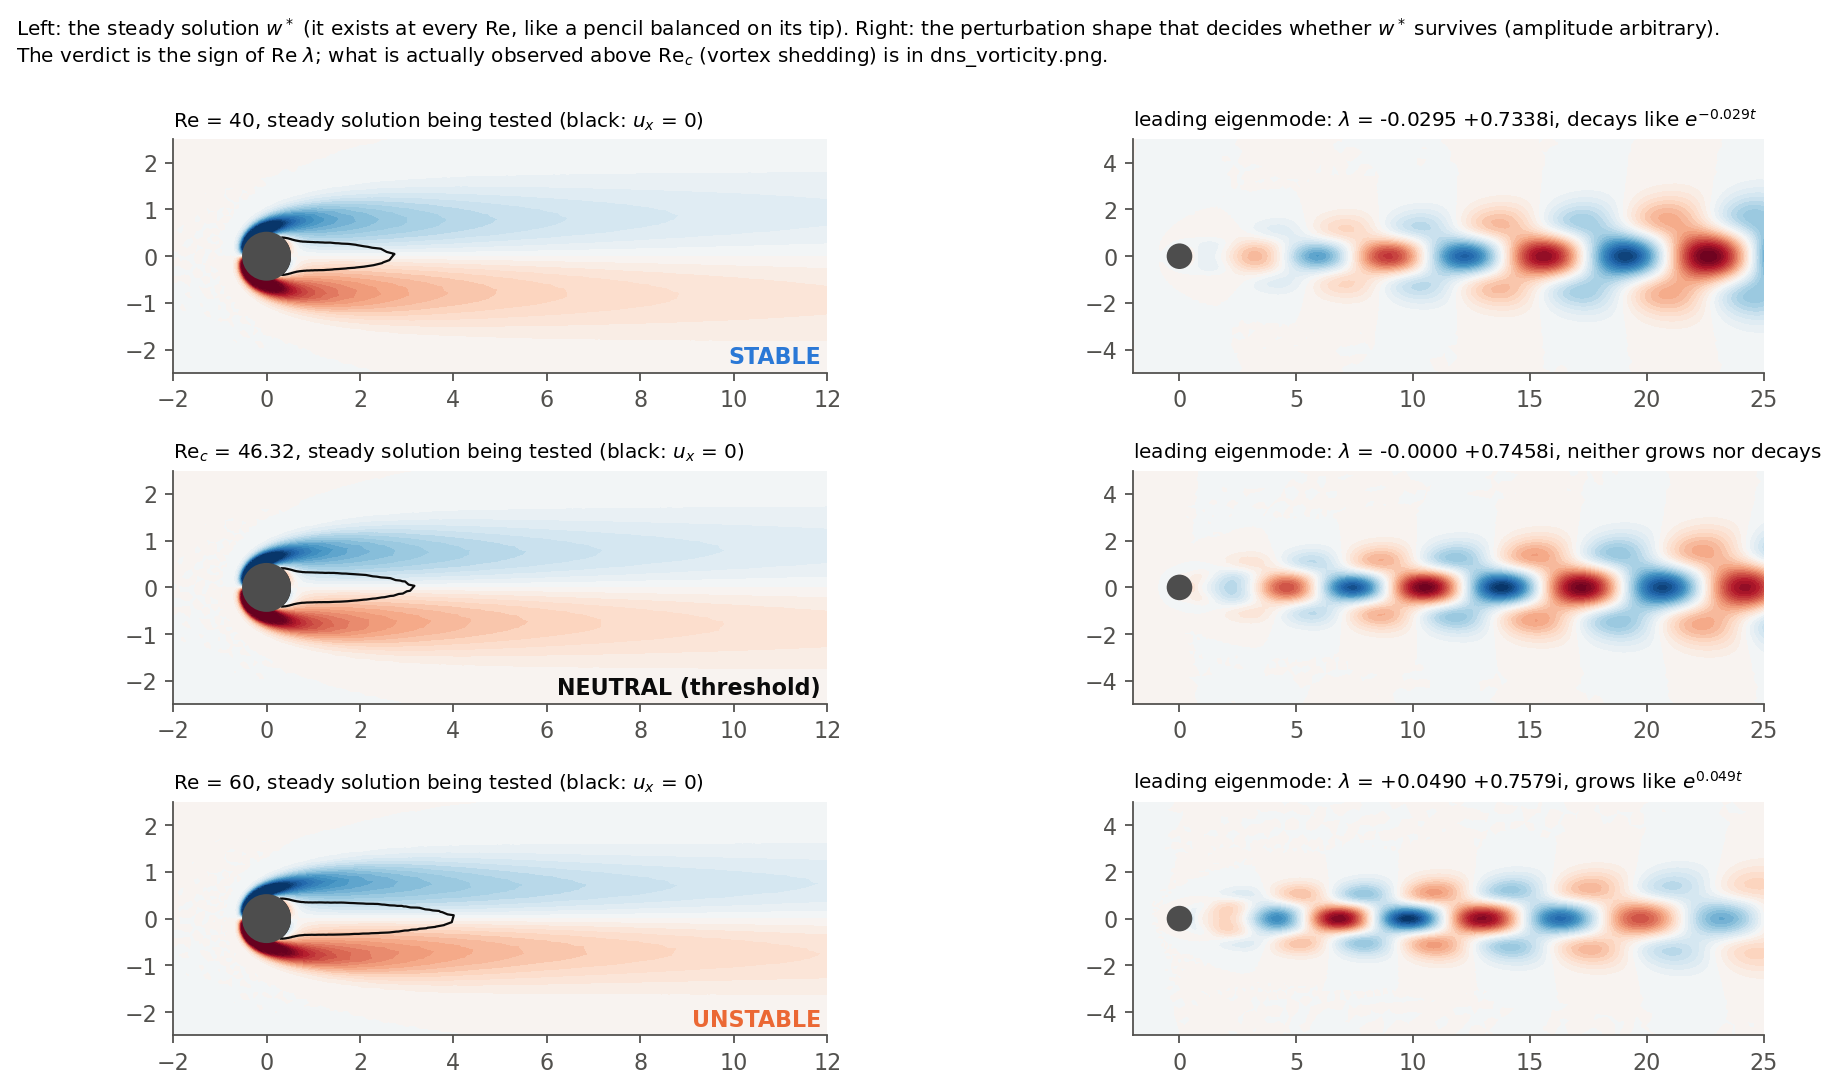
\includegraphics[width=\linewidth,height=182mm,keepaspectratio]{figures/wake_base_flow_and_eigenmode.png}\captionof{figure}[Archived figure]{Steady cylinder base flows and leading perturbations below, near, and above the Hopf threshold. The unstable symmetric steady solution is a valid base state even when nonlinear dynamics sheds vortices. \textit{Source:} \path{Ruben/Navier_Stokes_Inflow/stability/figures/base_flow_and_eigenmode.png}. First added 2026-09-29.}\end{center}
\clearpage
\begin{center}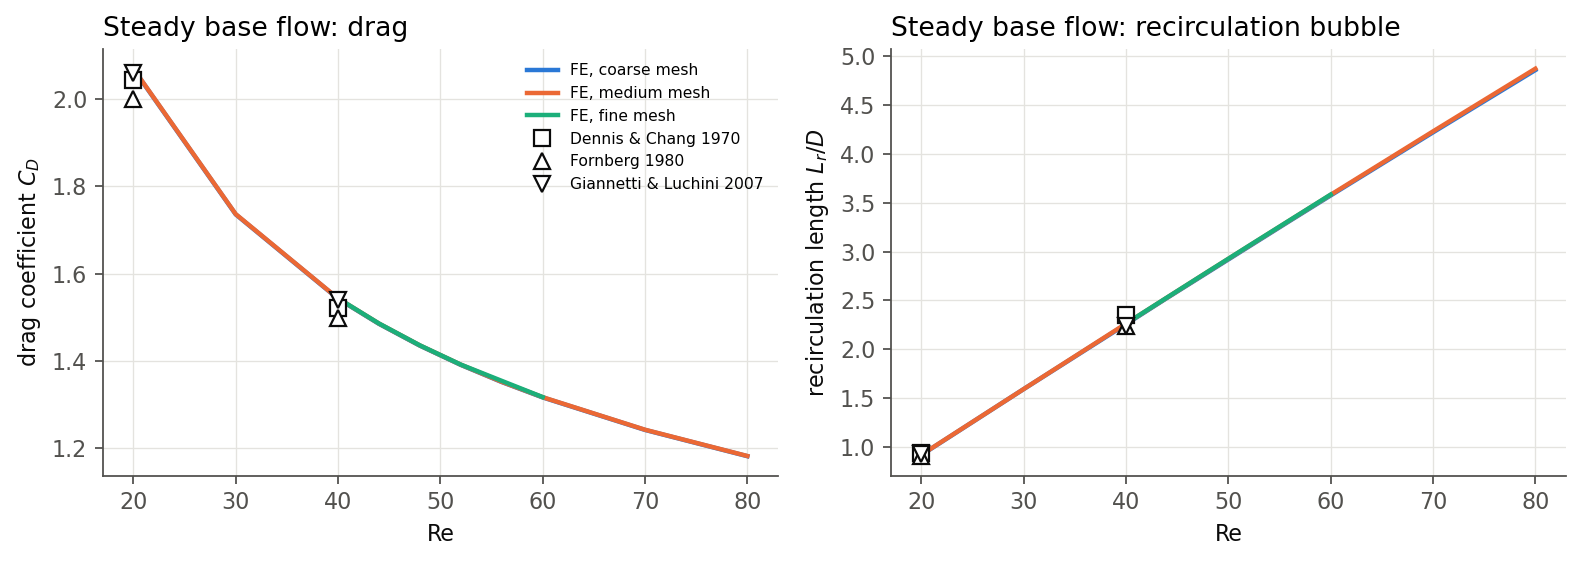
\includegraphics[width=\linewidth,height=86mm,keepaspectratio]{figures/wake_base_flow_validation.png}\captionof{figure}[Archived figure]{Cylinder drag and recirculation length compared with reference values. This tests the base solver independently of the eigensolver. \textit{Source:} \path{Ruben/Navier_Stokes_Inflow/stability/figures/base_flow_validation.png}. First added 2026-09-29.}\end{center}
\begin{center}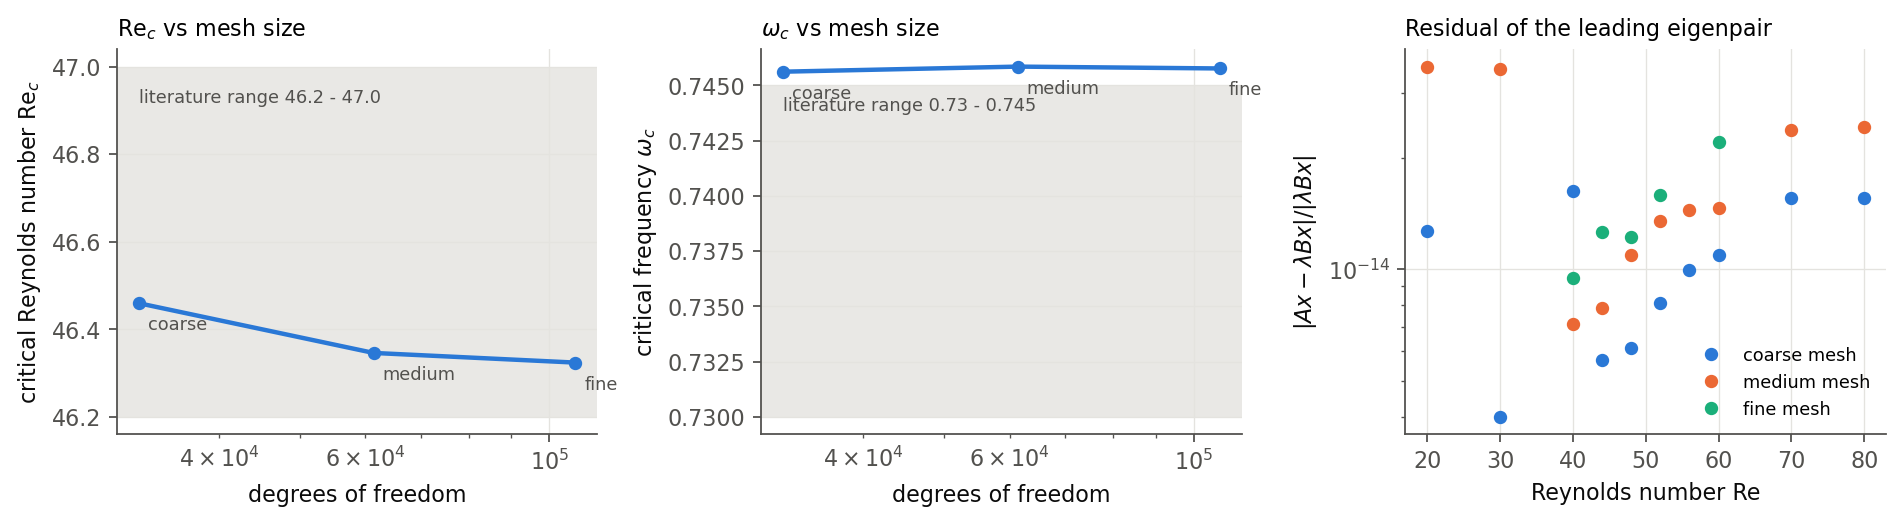
\includegraphics[width=\linewidth,height=86mm,keepaspectratio]{figures/wake_convergence_and_residuals.png}\captionof{figure}[Archived figure]{Cylinder onset, frequency, and eigenpair residuals under mesh refinement. The residual checks numerical solution of the discrete problem; mesh changes test its approximation to the continuum. \textit{Source:} \path{Ruben/Navier_Stokes_Inflow/stability/figures/convergence_and_residuals.png}. First added 2026-09-29.}\end{center}
\clearpage
\begin{center}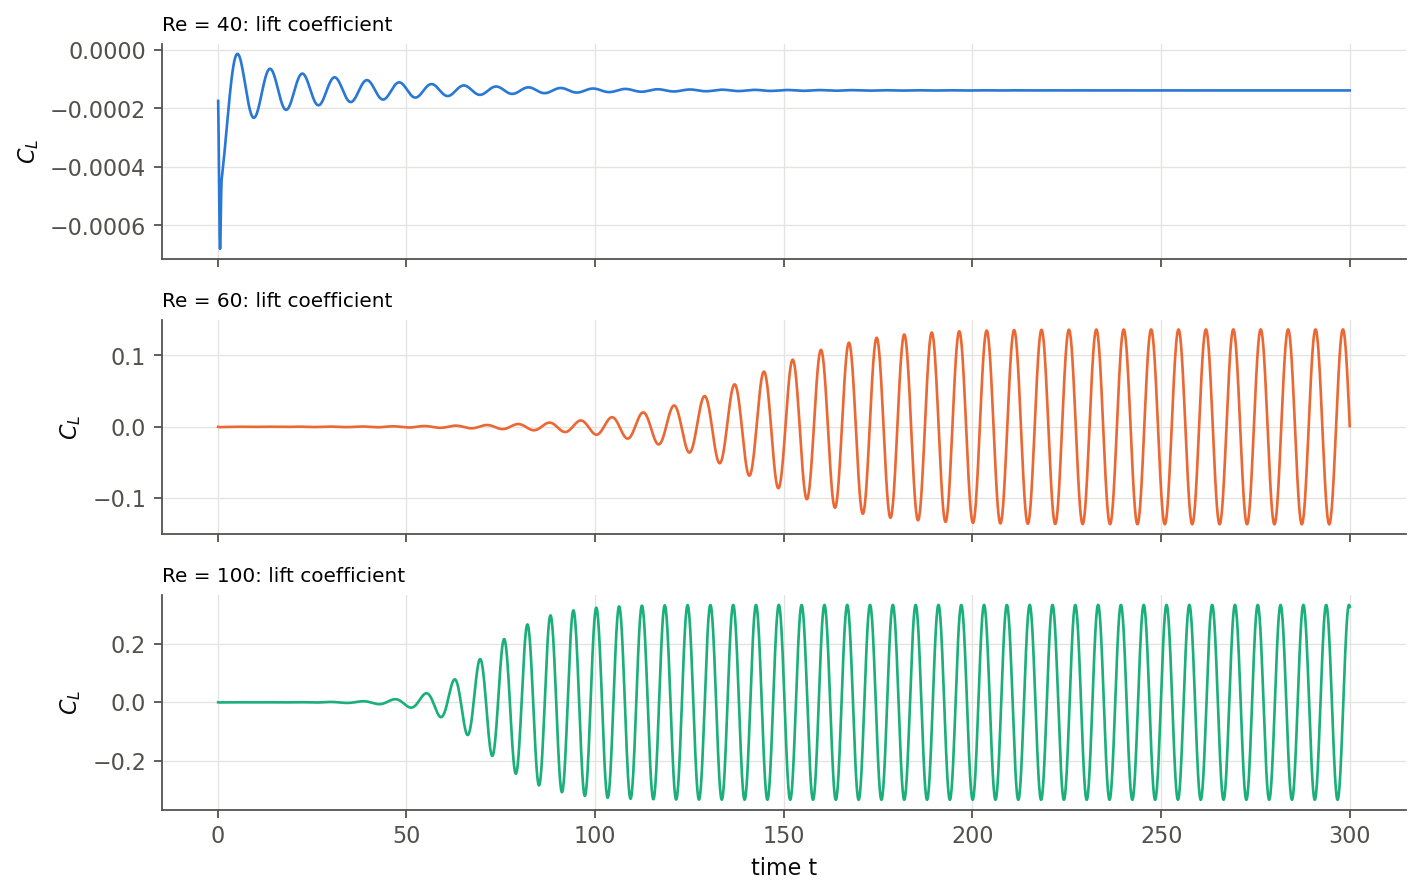
\includegraphics[width=\linewidth,height=182mm,keepaspectratio]{figures/wake_dns_lift.png}\captionof{figure}[Archived figure]{Lift time series at Reynolds numbers 40, 60, and 100. The low-Reynolds-number perturbation decays; the unstable cases grow and saturate in vortex shedding. \textit{Source:} \path{Ruben/Navier_Stokes_Inflow/stability/figures/dns_lift.png}. First added 2026-09-29.}\end{center}
\clearpage
\begin{center}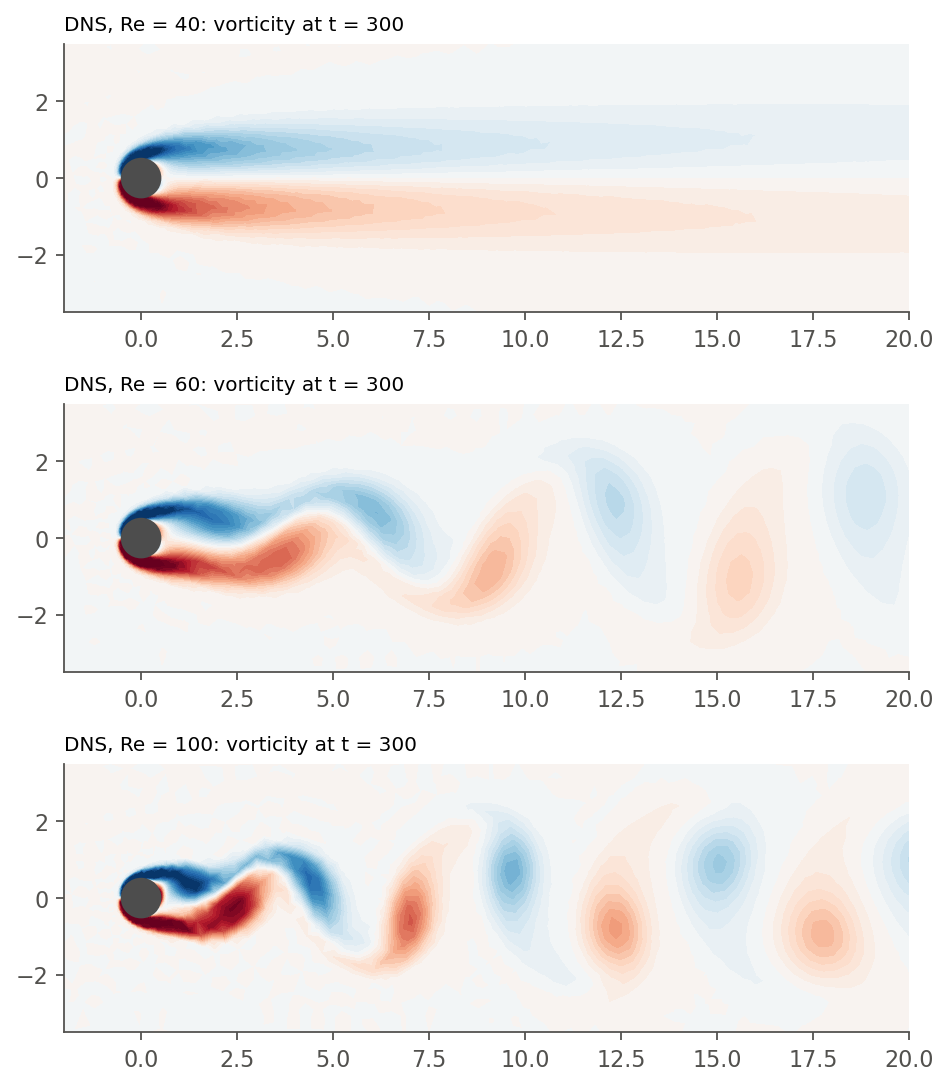
\includegraphics[width=\linewidth,height=182mm,keepaspectratio]{figures/wake_dns_vorticity.png}\captionof{figure}[Archived figure]{Nonlinear cylinder-wake snapshots for the benchmark runs. The vortex street above onset provides an independent dynamical check of the computed Hopf instability. \textit{Source:} \path{Ruben/Navier_Stokes_Inflow/stability/figures/dns_vorticity.png}. First added 2026-09-29.}\end{center}
\clearpage
\begin{center}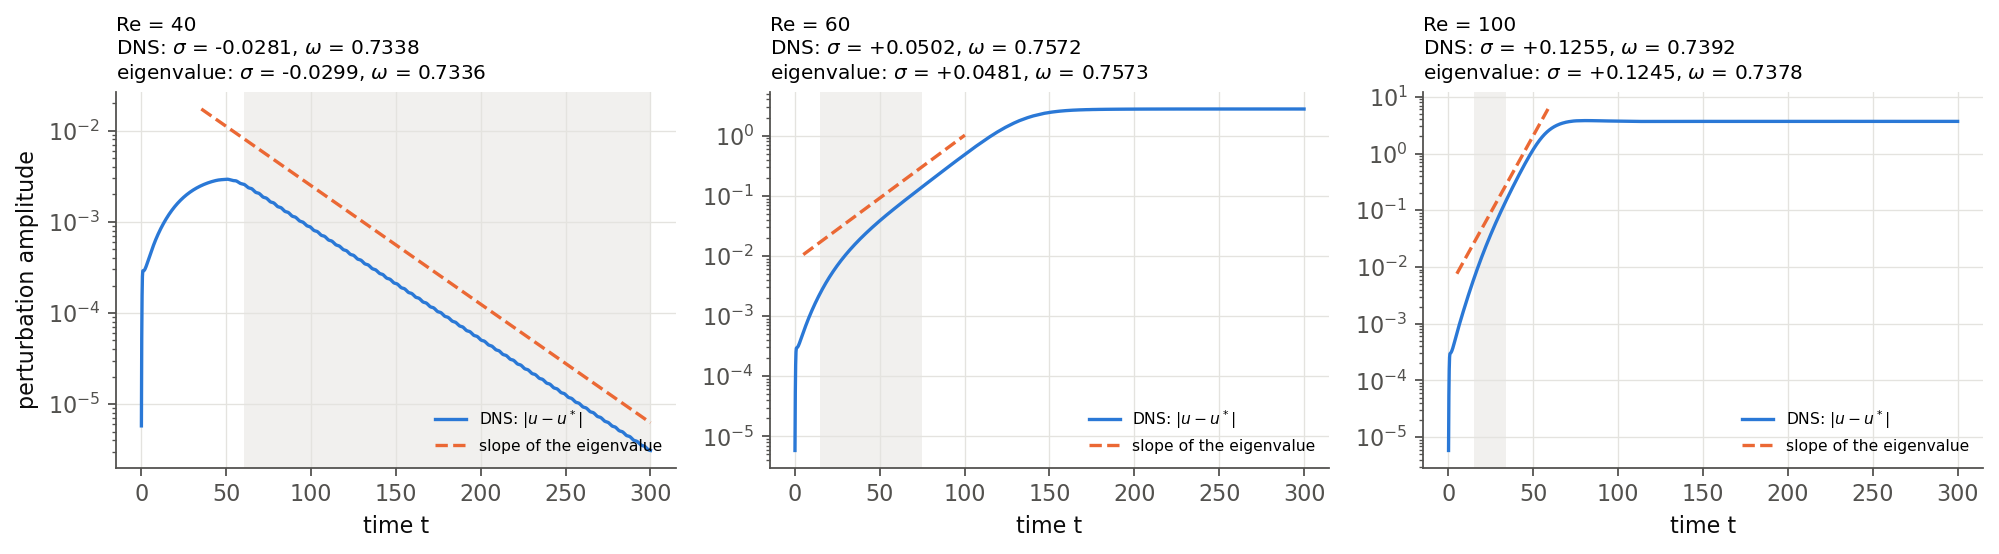
\includegraphics[width=\linewidth,height=182mm,keepaspectratio]{figures/wake_dns_vs_eigenvalues.png}\captionof{figure}[Archived figure]{Perturbation amplitude in cylinder DNS compared with exponential eigenvalue predictions. Growth is fitted in the linear interval before nonlinear saturation. \textit{Source:} \path{Ruben/Navier_Stokes_Inflow/stability/figures/dns_vs_eigenvalues.png}. First added 2026-09-29.}\end{center}
\clearpage
\begin{center}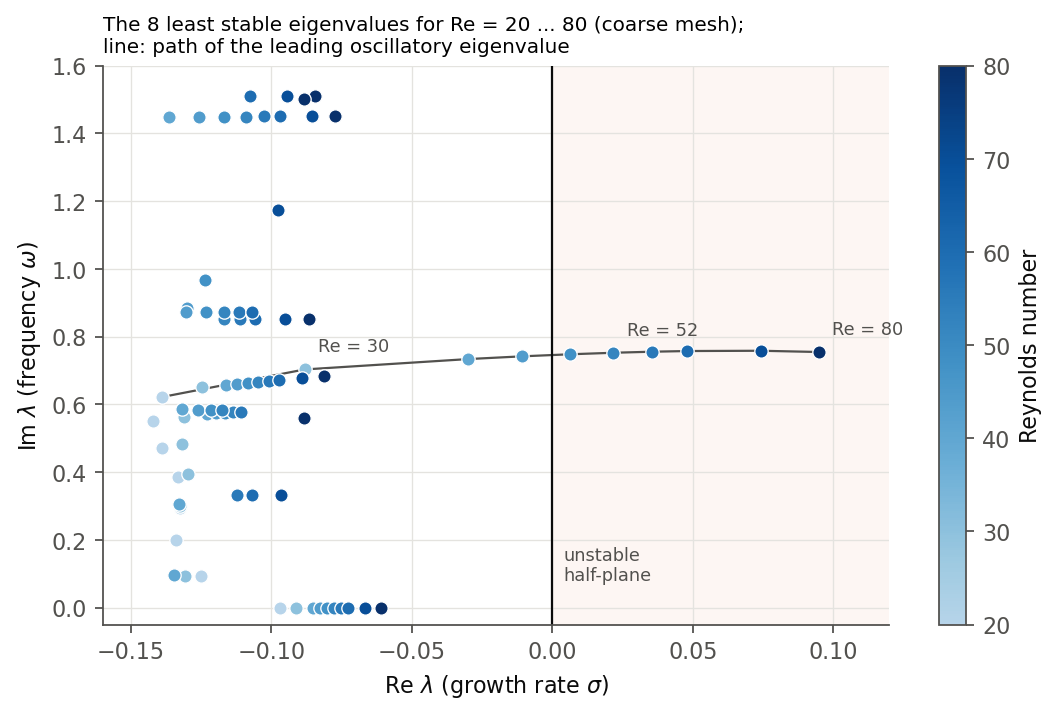
\includegraphics[width=\linewidth,height=182mm,keepaspectratio]{figures/wake_eigenvalue_trajectories.png}\captionof{figure}[Archived figure]{Cylinder eigenvalue trajectories as Reynolds number varies. The relevant oscillatory pair can be missed by searching only near the origin. \textit{Source:} \path{Ruben/Navier_Stokes_Inflow/stability/figures/eigenvalue_trajectories.png}. First added 2026-09-29.}\end{center}
\clearpage
\begin{center}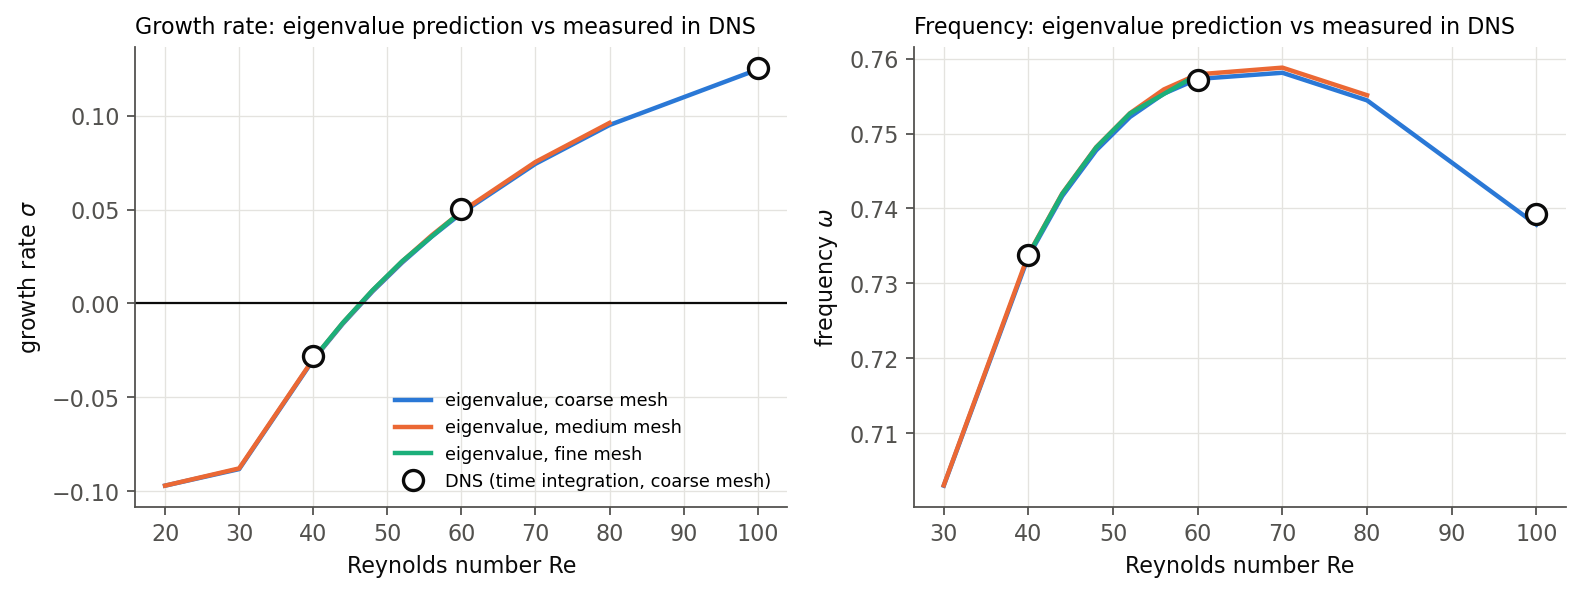
\includegraphics[width=\linewidth,height=86mm,keepaspectratio]{figures/wake_eigenvalues_vs_dns.png}\captionof{figure}[Archived figure]{Cylinder growth rates and frequencies from eigenanalysis and nonlinear time integration. Agreement is strongest for frequency and within a few percent for the fitted growth rates. \textit{Source:} \path{Ruben/Navier_Stokes_Inflow/stability/figures/eigenvalues_vs_dns.png}. First added 2026-09-29.}\end{center}
\begin{center}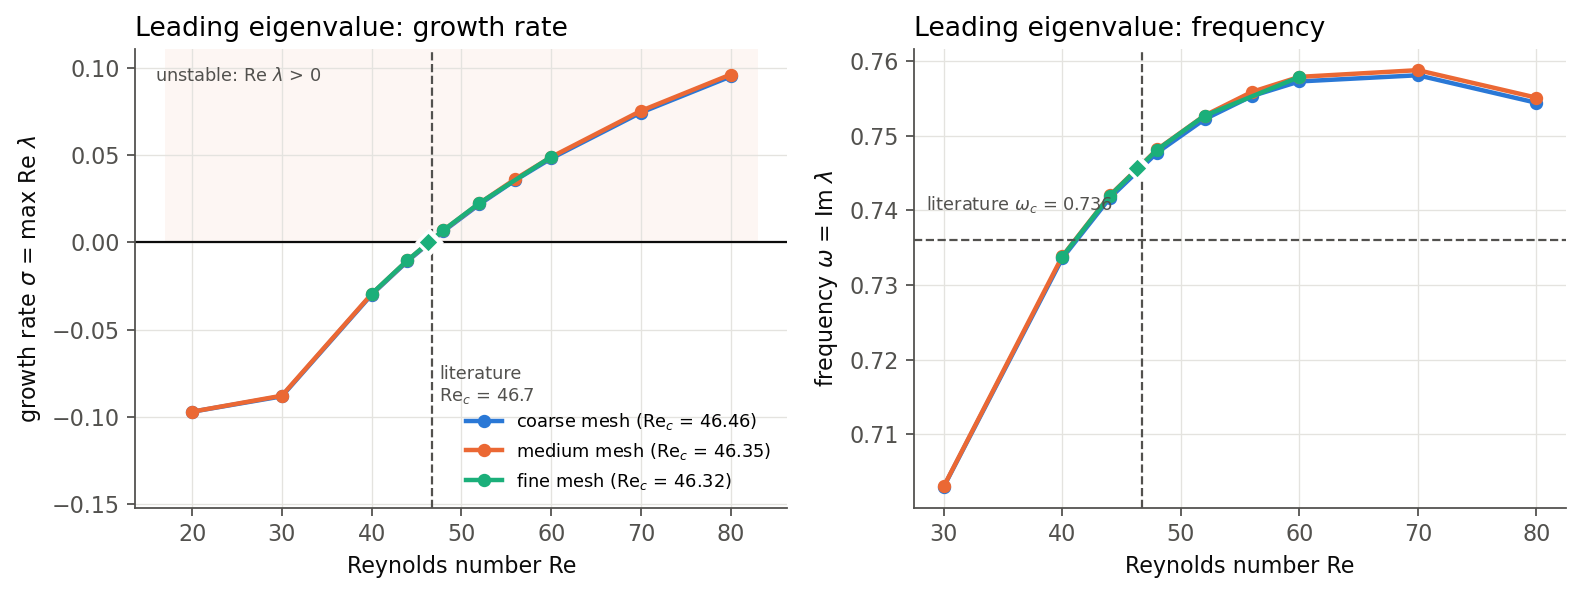
\includegraphics[width=\linewidth,height=86mm,keepaspectratio]{figures/wake_growth_rate_vs_Re.png}\captionof{figure}[Archived figure]{Leading cylinder growth rate and frequency versus Reynolds number on three meshes. The first instability occurs near Reynolds number 46.3. \textit{Source:} \path{Ruben/Navier_Stokes_Inflow/stability/figures/growth_rate_vs_Re.png}. First added 2026-09-29.}\end{center}
\clearpage
\begin{center}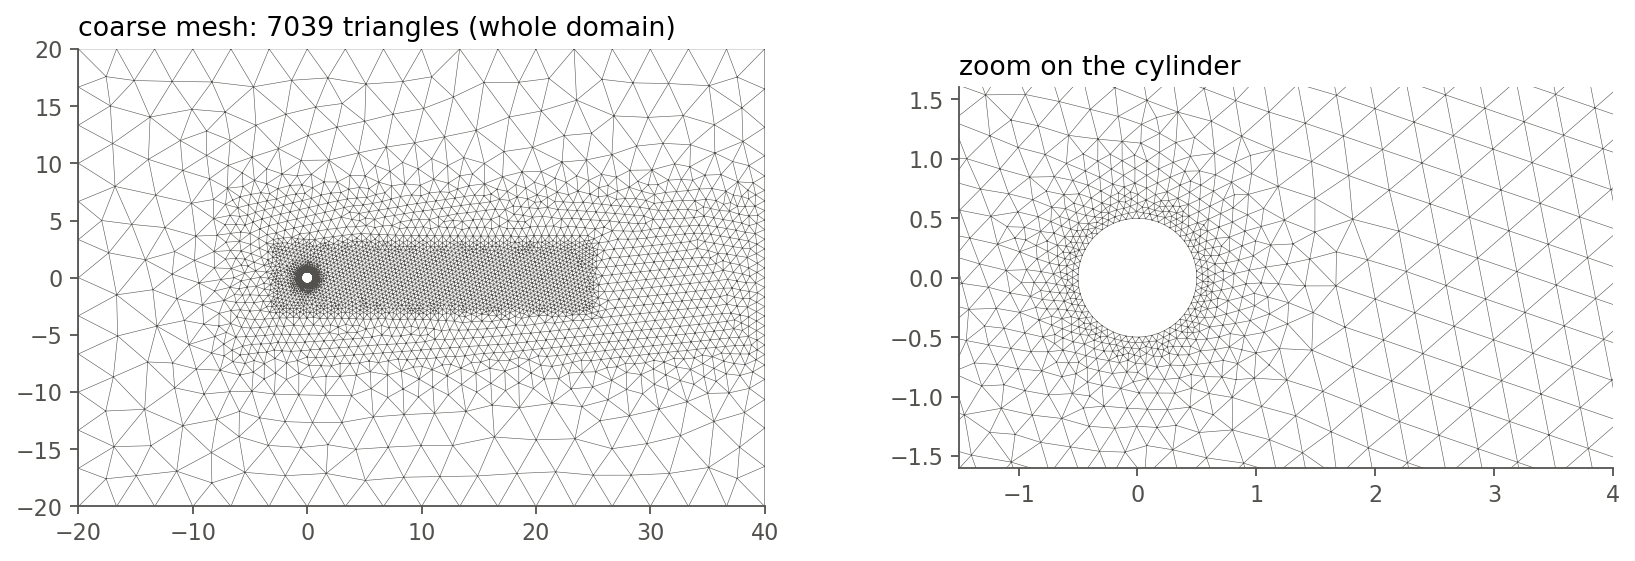
\includegraphics[width=\linewidth,height=86mm,keepaspectratio]{figures/wake_mesh_coarse.png}\captionof{figure}[Archived figure]{Coarse cylinder mesh, including a close view of the obstacle. This is the first of the three benchmark resolutions. \textit{Source:} \path{Ruben/Navier_Stokes_Inflow/stability/figures/mesh_coarse.png}. First added 2026-09-29.}\end{center}
\begin{center}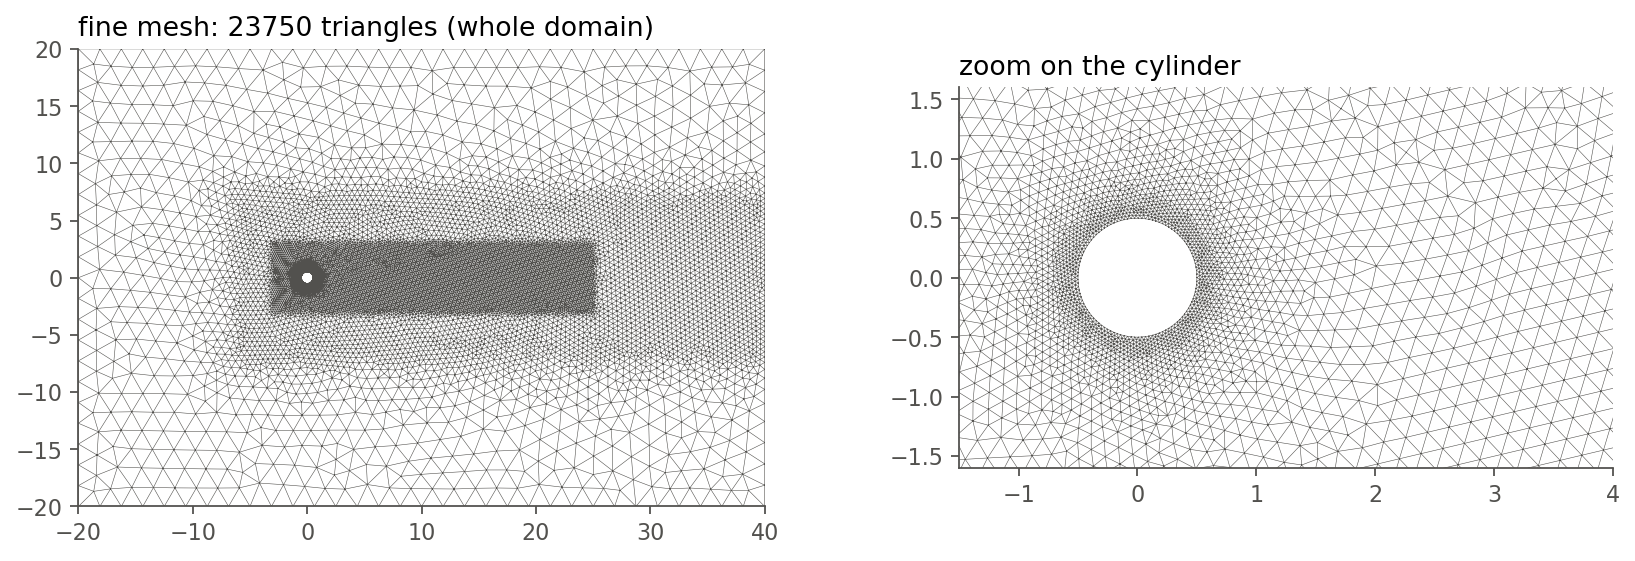
\includegraphics[width=\linewidth,height=86mm,keepaspectratio]{figures/wake_mesh_fine.png}\captionof{figure}[Archived figure]{Fine cylinder mesh and obstacle refinement. It gives the reported benchmark onset near Reynolds number 46.32. \textit{Source:} \path{Ruben/Navier_Stokes_Inflow/stability/figures/mesh_fine.png}. First added 2026-09-29.}\end{center}
\clearpage
\begin{center}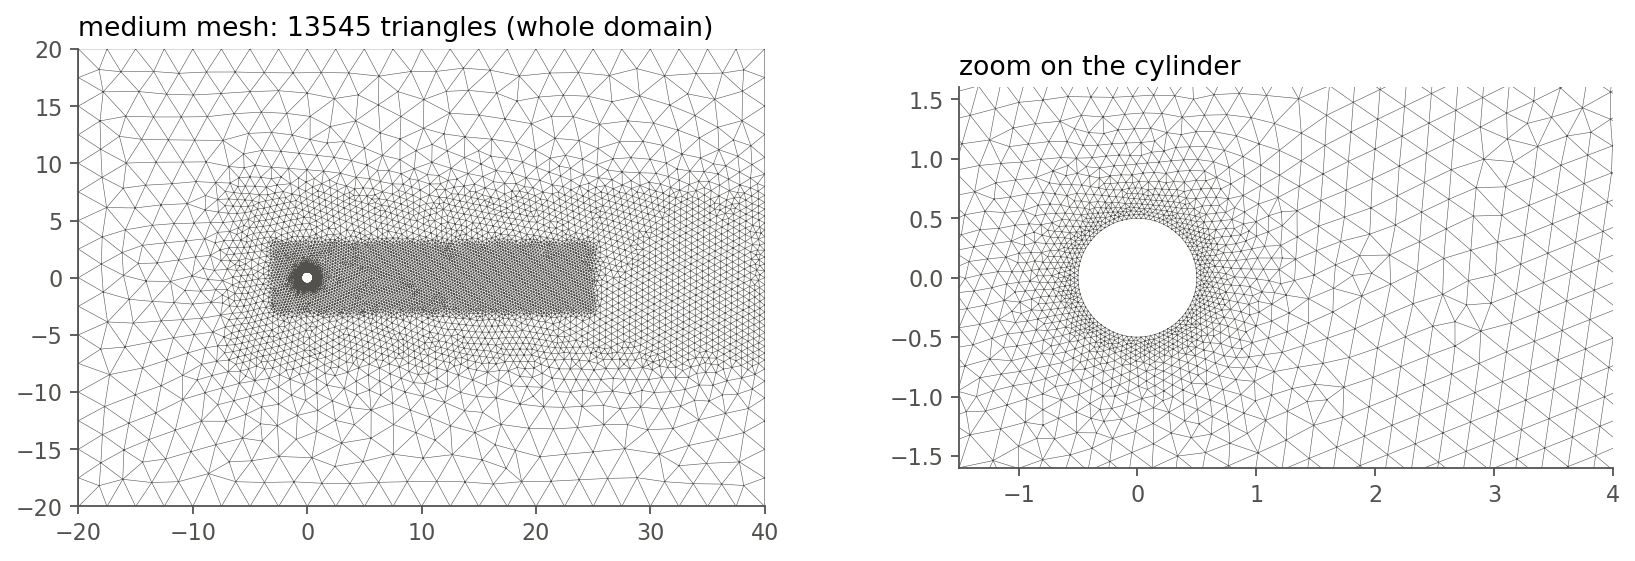
\includegraphics[width=\linewidth,height=86mm,keepaspectratio]{figures/wake_mesh_medium.png}\captionof{figure}[Archived figure]{Intermediate cylinder mesh and obstacle refinement. It supplies the middle point of the convergence sequence. \textit{Source:} \path{Ruben/Navier_Stokes_Inflow/stability/figures/mesh_medium.png}. First added 2026-09-29.}\end{center}
\begin{center}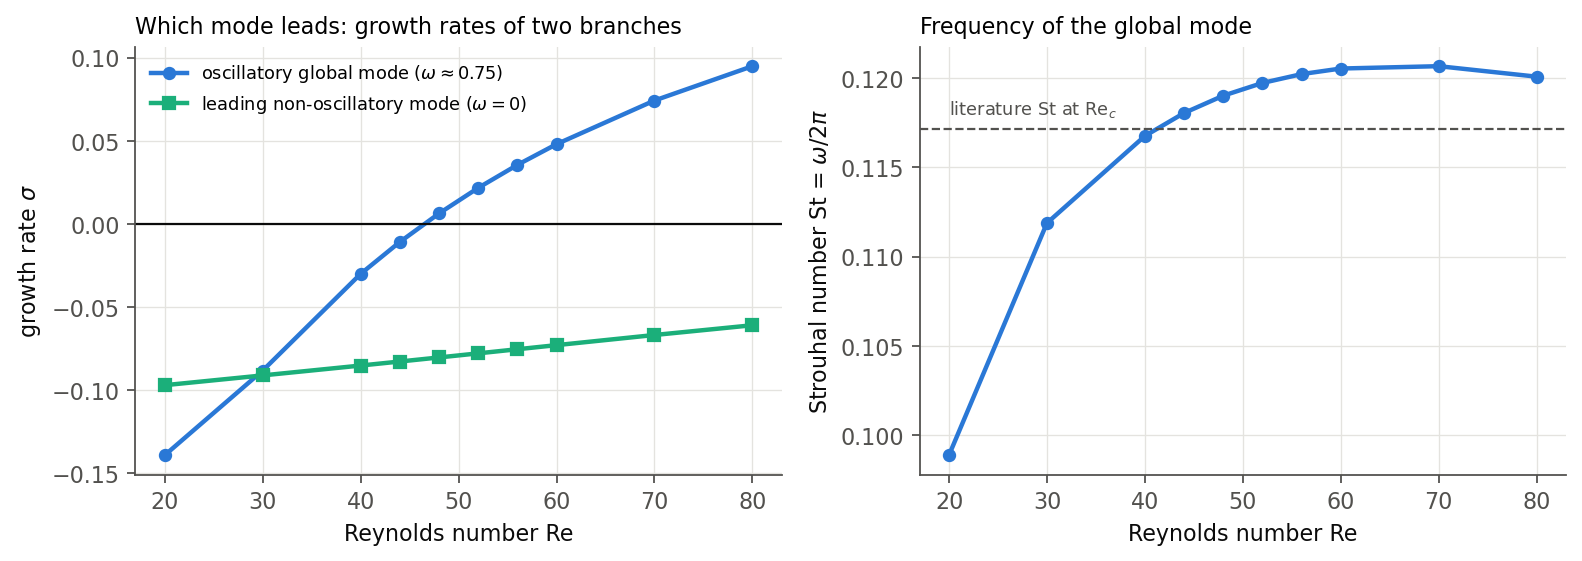
\includegraphics[width=\linewidth,height=86mm,keepaspectratio]{figures/wake_mode_branches_vs_Re.png}\captionof{figure}[Archived figure]{Competing cylinder growth-rate branches and the leading Hopf Strouhal number. Selecting the least damped returned eigenpair requires covering the relevant complex-frequency range. \textit{Source:} \path{Ruben/Navier_Stokes_Inflow/stability/figures/mode_branches_vs_Re.png}. First added 2026-09-29.}\end{center}
\clearpage
\begin{center}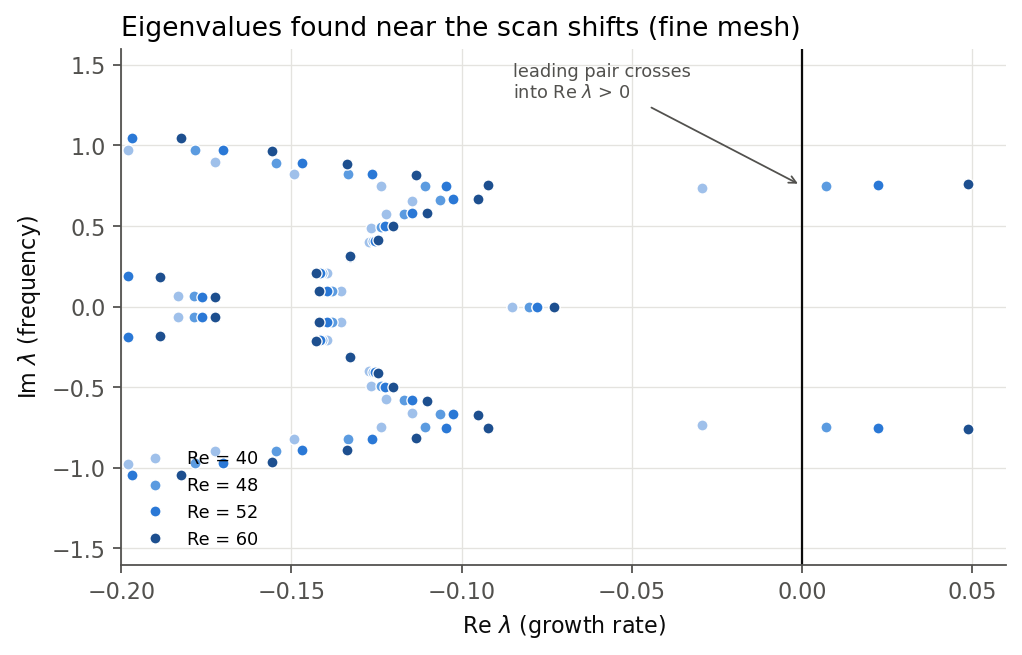
\includegraphics[width=\linewidth,height=182mm,keepaspectratio]{figures/wake_spectra.png}\captionof{figure}[Archived figure]{Cylinder spectra near the sampled complex shifts. The Hopf pair and dense damped cluster illustrate why a real shift alone is insufficient. \textit{Source:} \path{Ruben/Navier_Stokes_Inflow/stability/figures/spectra.png}. First added 2026-09-29.}\end{center}
\clearpage
\begin{center}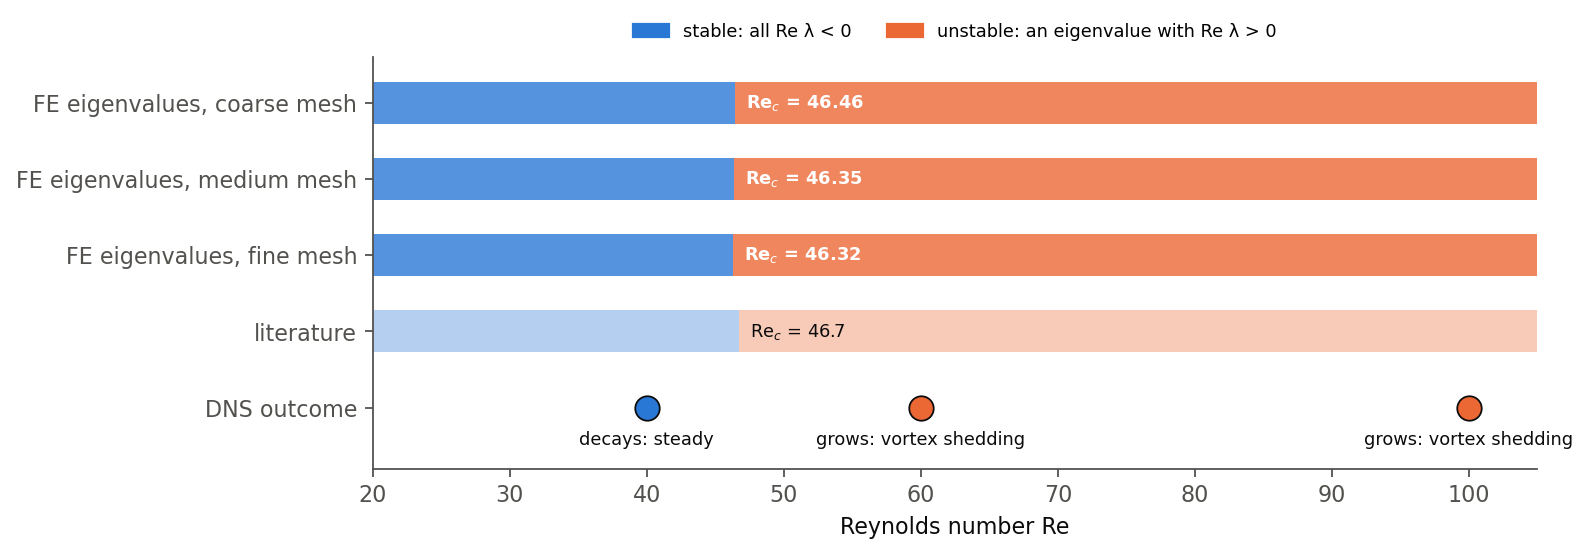
\includegraphics[width=\linewidth,height=86mm,keepaspectratio]{figures/wake_stability_map.png}\captionof{figure}[Archived figure]{Cylinder stable/unstable classification from eigenvalues and independent DNS outcomes. Threshold differences across meshes are small but remain measurable. \textit{Source:} \path{Ruben/Navier_Stokes_Inflow/stability/figures/stability_map.png}. First added 2026-09-29.}\end{center}
\begin{center}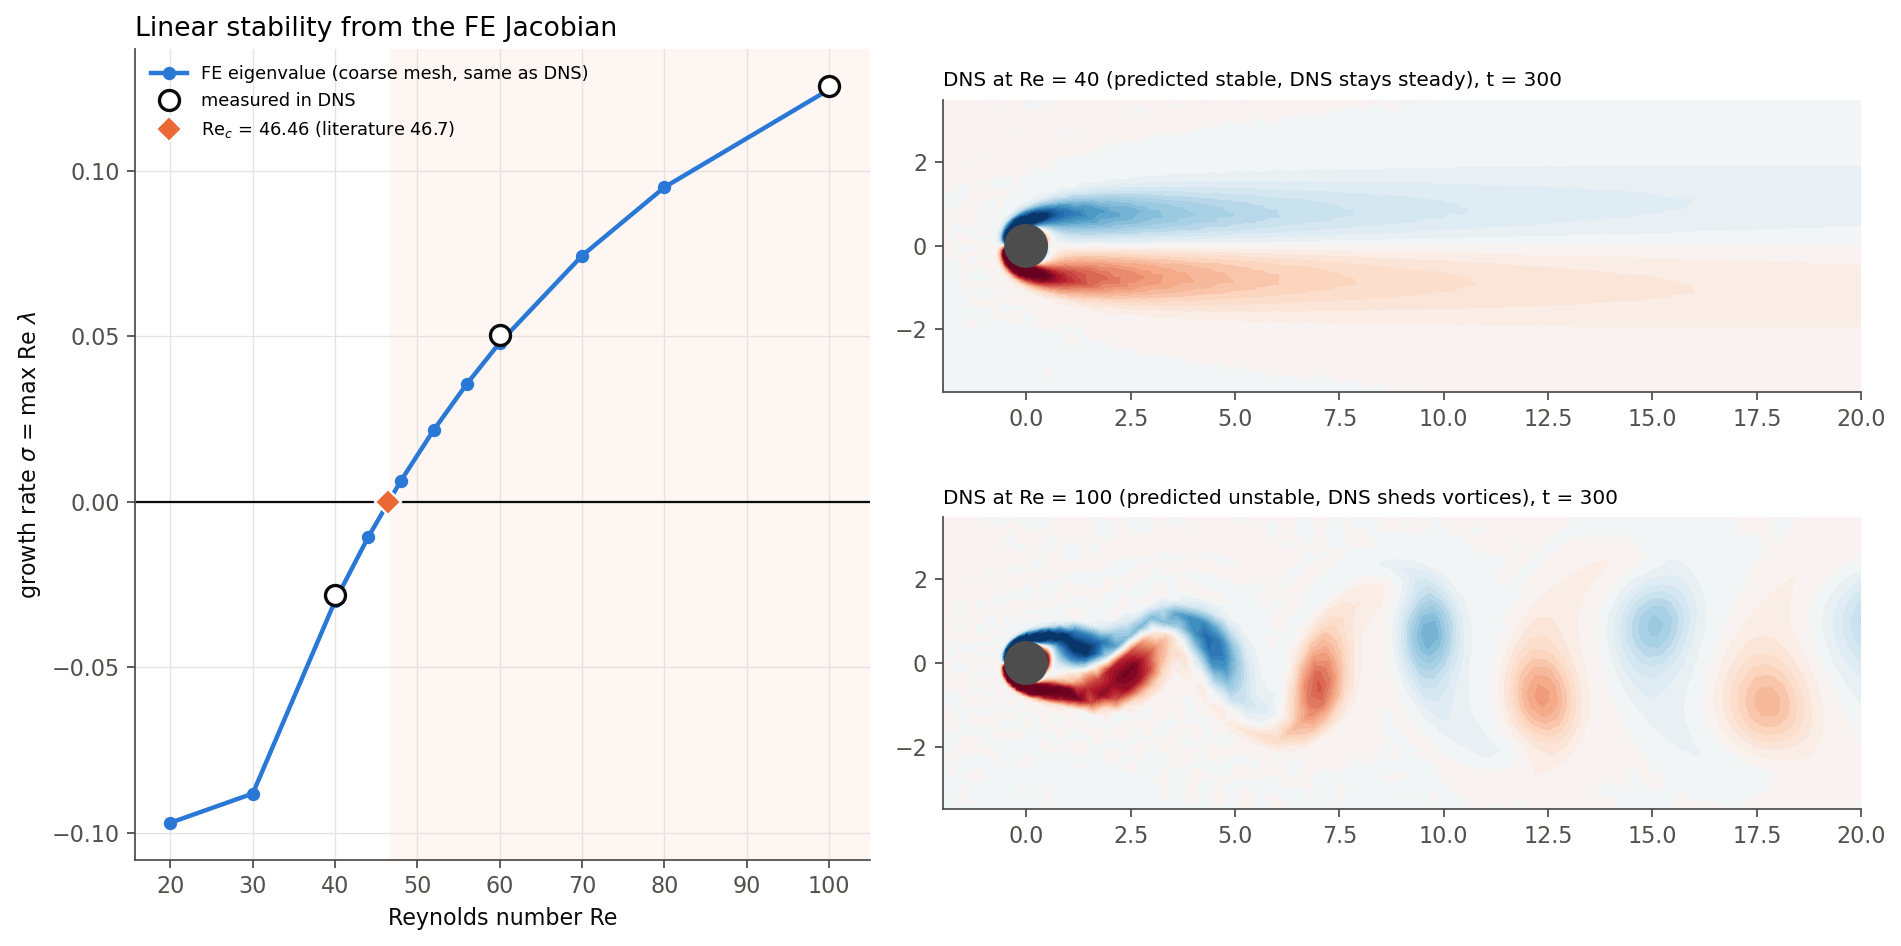
\includegraphics[width=\linewidth,height=86mm,keepaspectratio]{figures/wake_summary.png}\captionof{figure}[Archived figure]{Overview of the cylinder benchmark: leading growth rate, threshold, and contrasting nonlinear outcomes below and above onset. \textit{Source:} \path{Ruben/Navier_Stokes_Inflow/stability/figures/summary.png}. First added 2026-09-29.}\end{center}
\clearpage
\begin{center}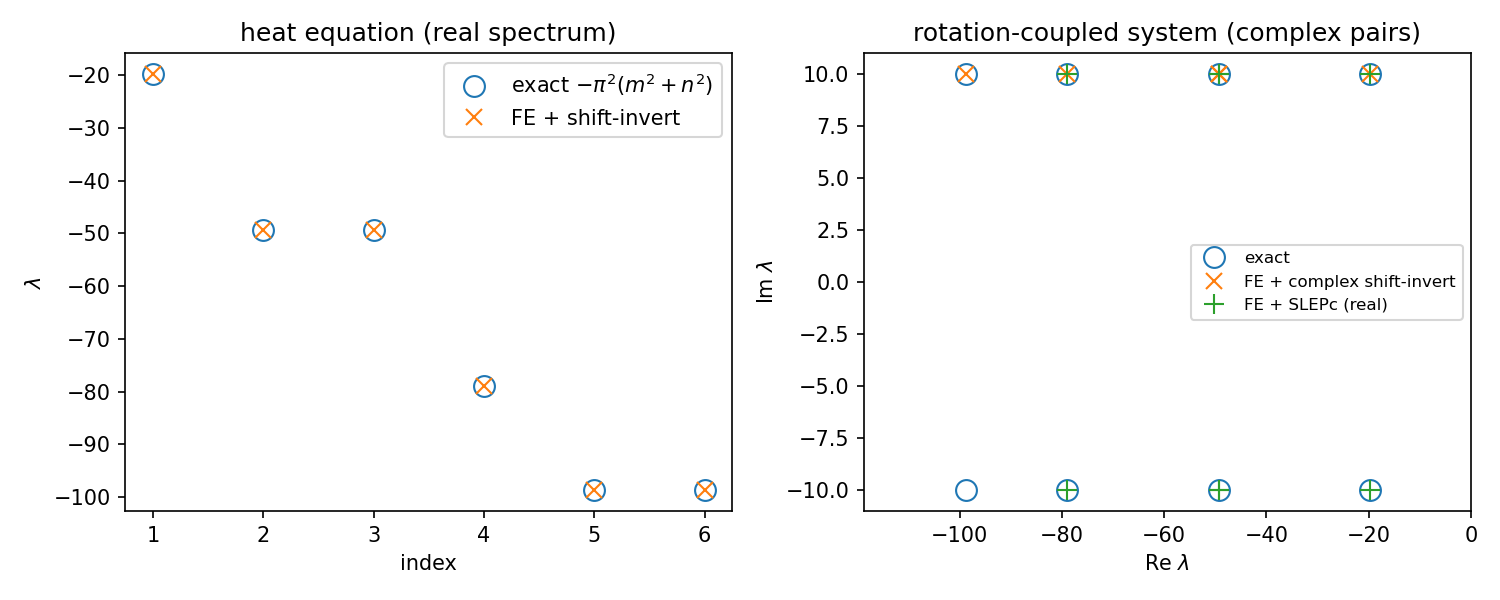
\includegraphics[width=\linewidth,height=182mm,keepaspectratio]{figures/wake_check_eigensolver.png}\captionof{figure}[Archived figure]{Generic eigensolver checks on a heat equation and a rotation-coupled system with complex eigenpairs. Both real and complex spectral calculations are tested against exact values. \textit{Source:} \path{Ruben/Navier_Stokes_Inflow/stability/solution/checks/check_eigensolver.png}. First added 2026-09-29.}\end{center}
\clearpage
\begin{center}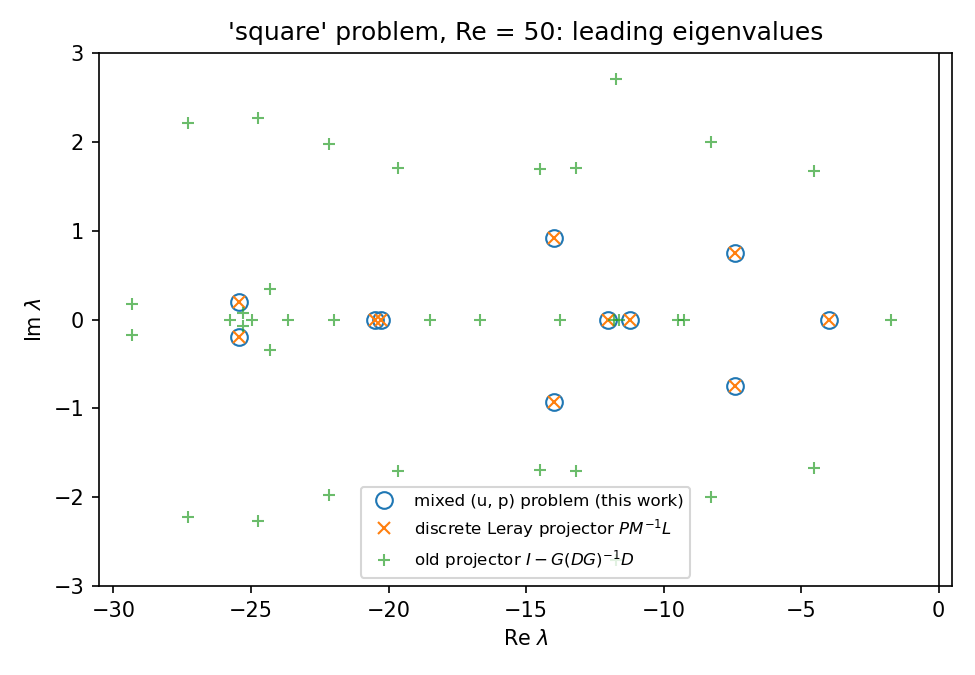
\includegraphics[width=\linewidth,height=182mm,keepaspectratio]{figures/wake_check_projector_equivalence.png}\captionof{figure}[Archived figure]{Mixed incompressible eigenproblem compared with the correct discrete Leray projector. A Euclidean projector is a different operator and produces different spectra. \textit{Source:} \path{Ruben/Navier_Stokes_Inflow/stability/solution/checks/check_projector_equivalence.png}. First added 2026-09-29.}\end{center}
\clearpage
\begin{center}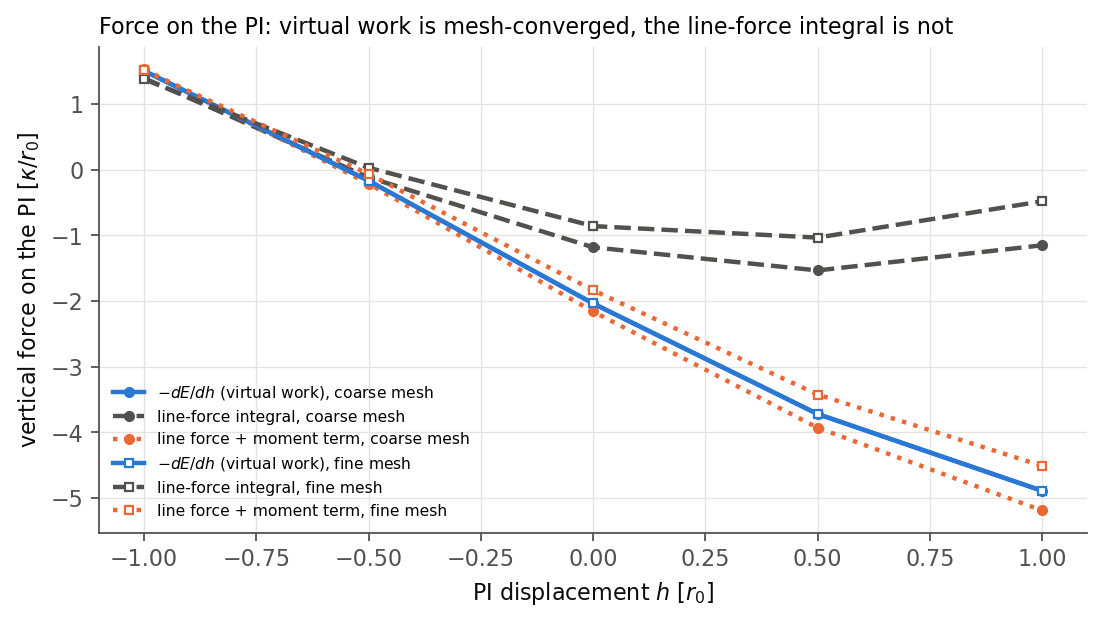
\includegraphics[width=\linewidth,height=182mm,keepaspectratio]{figures/membrane_check_force_methods.png}\captionof{figure}[Archived figure]{Ring force diagnostic under refinement. Virtual work converges; the original boundary line integral does not. Adding the moment term improves a coarse result but does not remove the boundary-derivative discretization error. \textit{Source:} \path{Ruben/membrane_stability/figures/check_force_methods.png}. First added 2026-09-29.}\end{center}
\clearpage
\begin{center}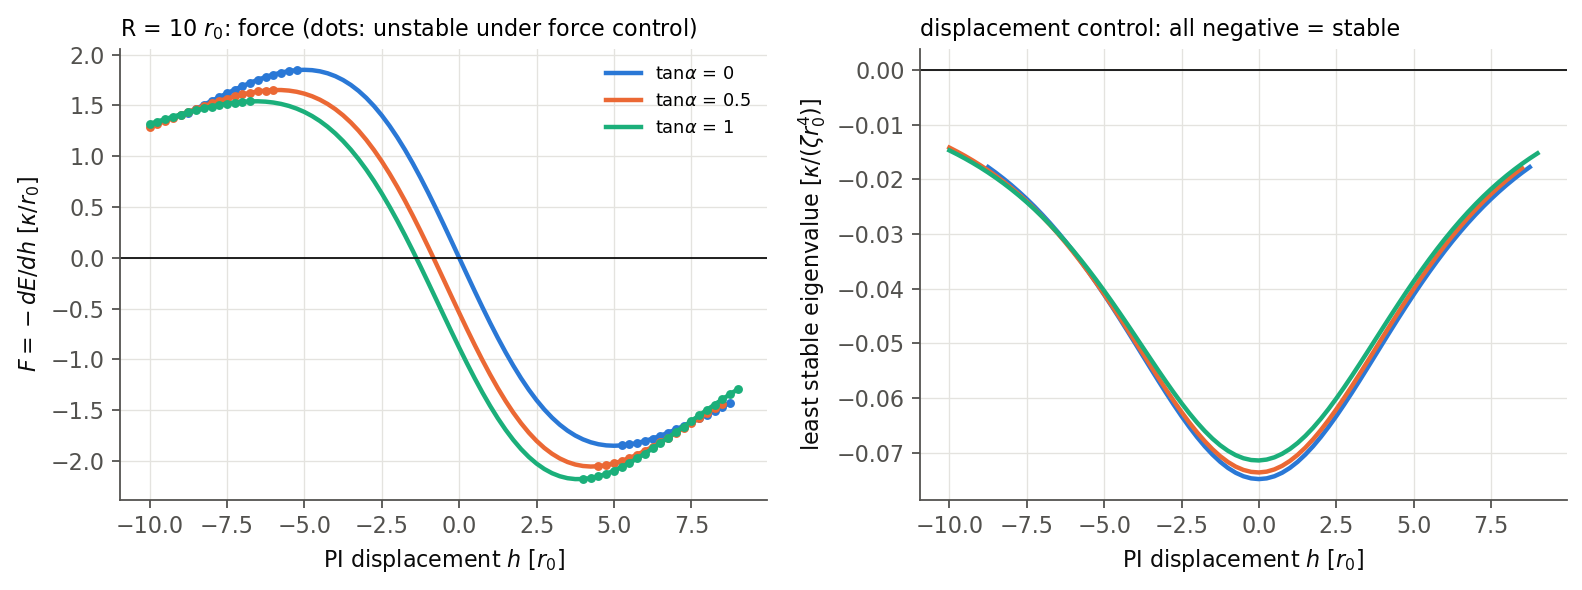
\includegraphics[width=\linewidth,height=86mm,keepaspectratio]{figures/membrane_contact_angle_R10.png}\captionof{figure}[Archived figure]{Contact-slope dependence of ring force and leading relaxation rate at outer radius ten. Force extrema shift, while the sampled height-controlled branches remain stable. \textit{Source:} \path{Ruben/membrane_stability/figures/contact_angle_R10.png}. First added 2026-09-29.}\end{center}
\begin{center}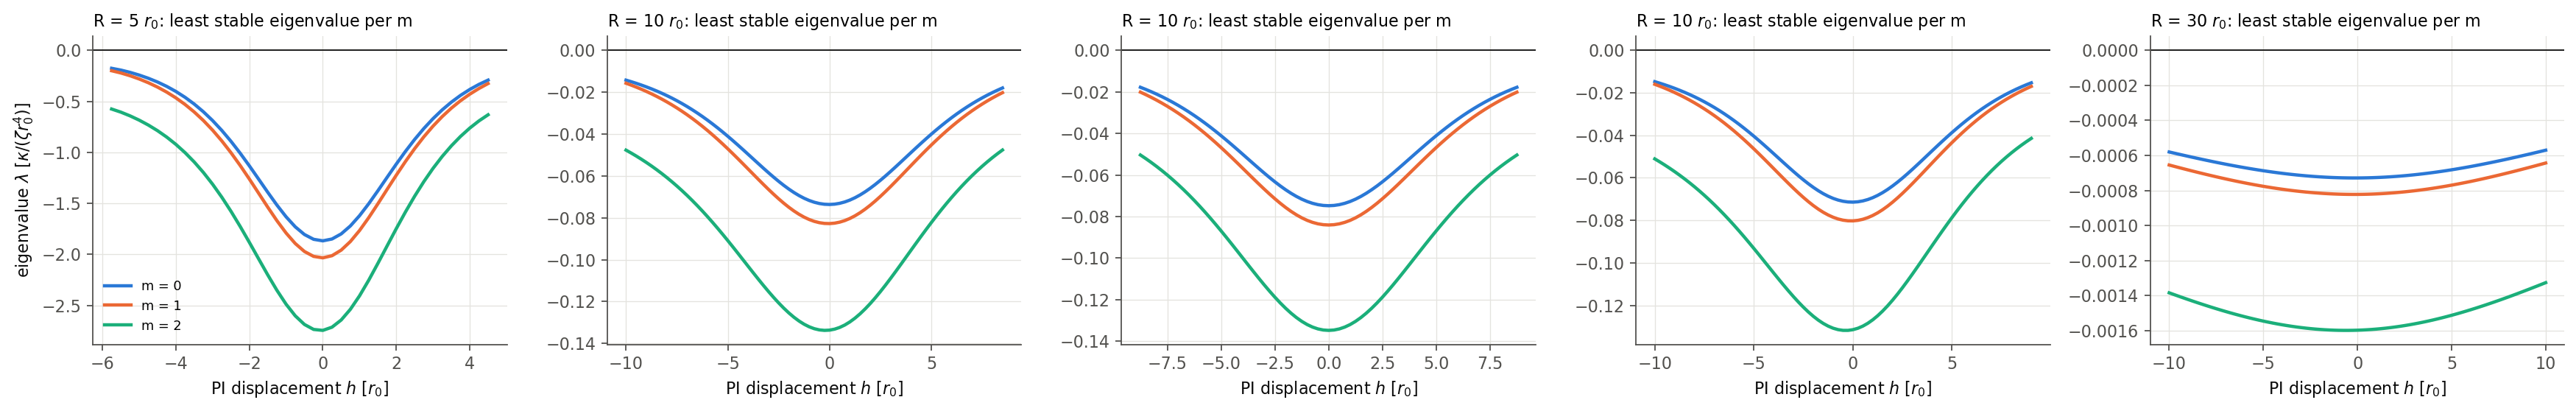
\includegraphics[width=\linewidth,height=86mm,keepaspectratio]{figures/membrane_eigenvalues_vs_h.png}\captionof{figure}[Archived figure]{Ring relaxation spectra versus protein height, resolved by azimuthal number. No growing fixed-height mode is found in these sampled branches; spectra soften as the neck becomes steep. \textit{Source:} \path{Ruben/membrane_stability/figures/eigenvalues_vs_h.png}. First added 2026-09-29.}\end{center}
\clearpage
\begin{center}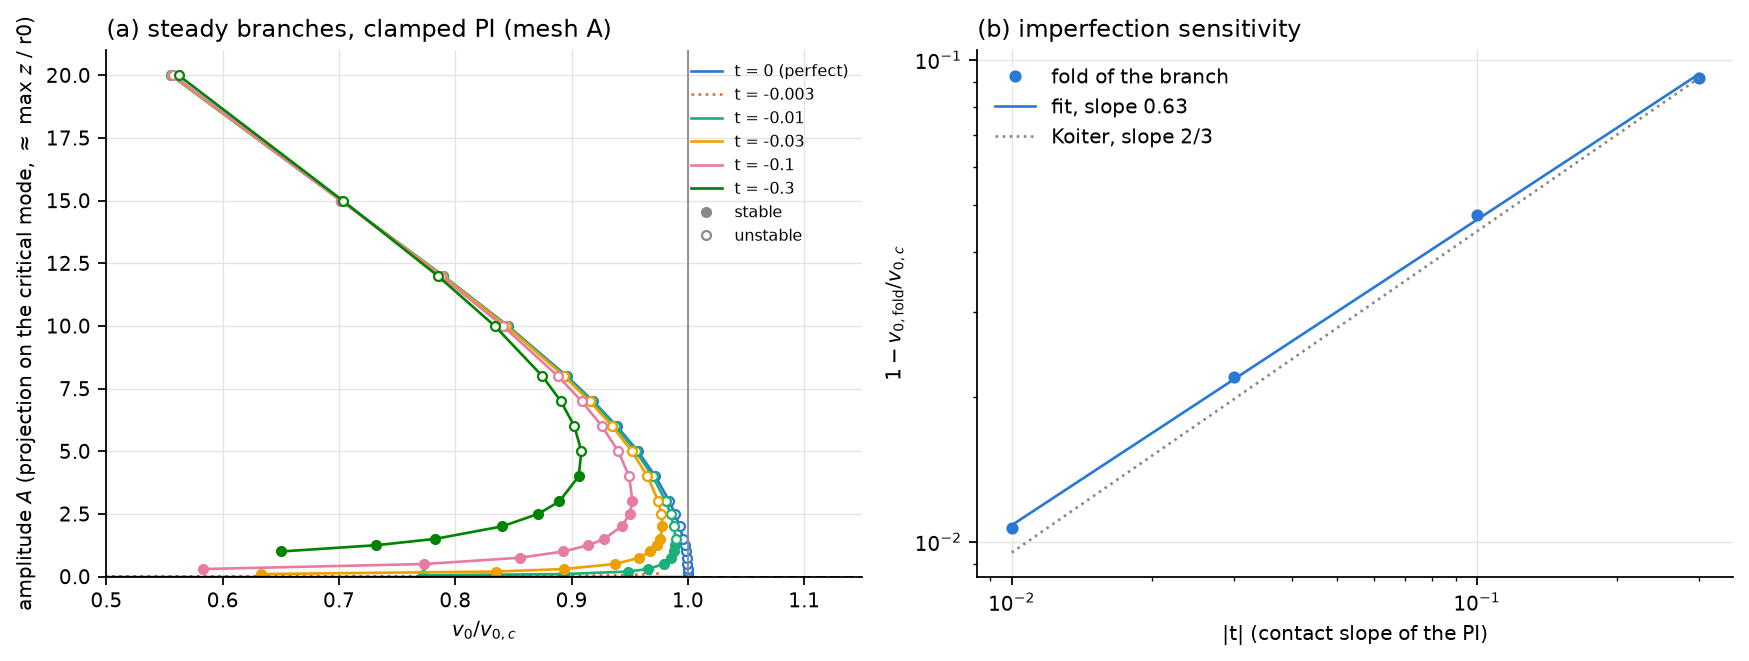
\includegraphics[width=\linewidth,height=86mm,keepaspectratio]{figures/membrane_flow2_bifurcation.png}\captionof{figure}[Archived figure]{Corrected clamped-protein continuation. The perfect branch is subcritical and a nonzero contact slope produces a fold; the fitted imperfection exponent is close to two thirds. The later projected theory supplies an independently computed prefactor. \textit{Source:} \path{Ruben/membrane_stability/figures/flow2_bifurcation.png}. First added 2026-09-30.}\end{center}
\begin{center}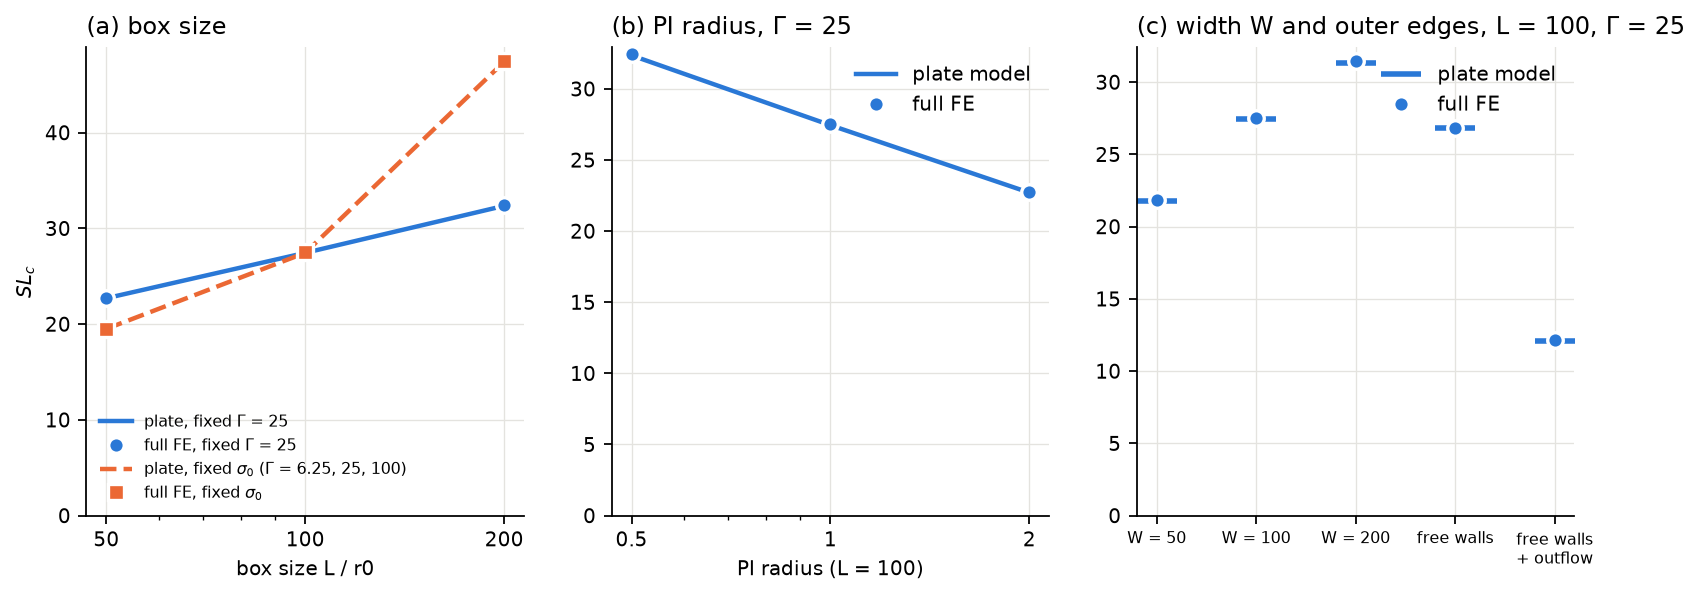
\includegraphics[width=\linewidth,height=86mm,keepaspectratio]{figures/membrane_flow2_domain.png}\captionof{figure}[Archived figure]{Corrected physical thresholds versus domain length, protein radius, width, and outer-height constraints. Fixed-tension and fixed-Gamma size sweeps are different experiments. \textit{Source:} \path{Ruben/membrane_stability/figures/flow2_domain.png}. First added 2026-09-30.}\end{center}
\clearpage
\begin{center}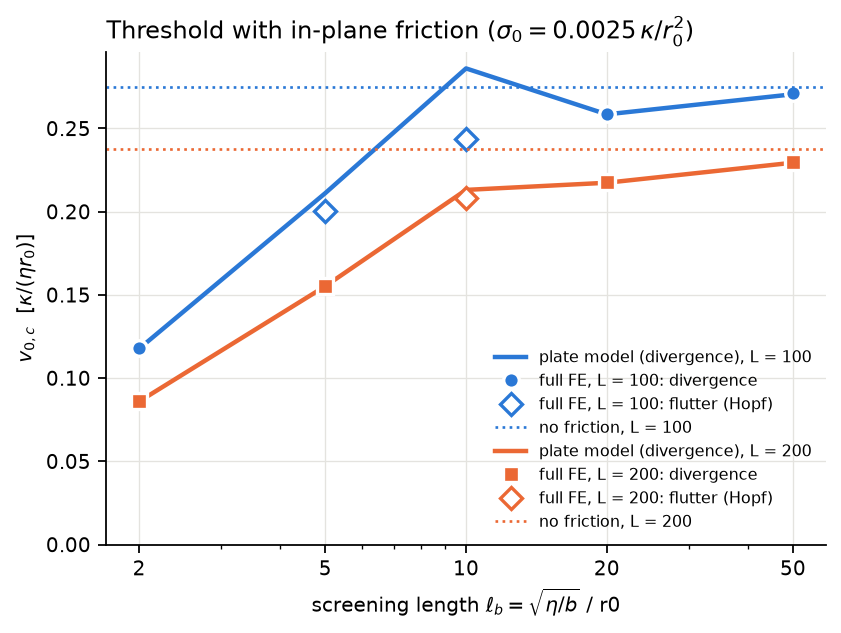
\includegraphics[width=\linewidth,height=182mm,keepaspectratio]{figures/membrane_flow2_friction.png}\captionof{figure}[Archived figure]{Early friction comparison showing divergence thresholds and full-equation flutter crossings. The real plate threshold curve alone is not the first onset when a complex pair crosses earlier; the later map in the archive resolves this. \textit{Source:} \path{Ruben/membrane_stability/figures/flow2_friction.png}. First added 2026-09-30.}\end{center}
\clearpage
\begin{center}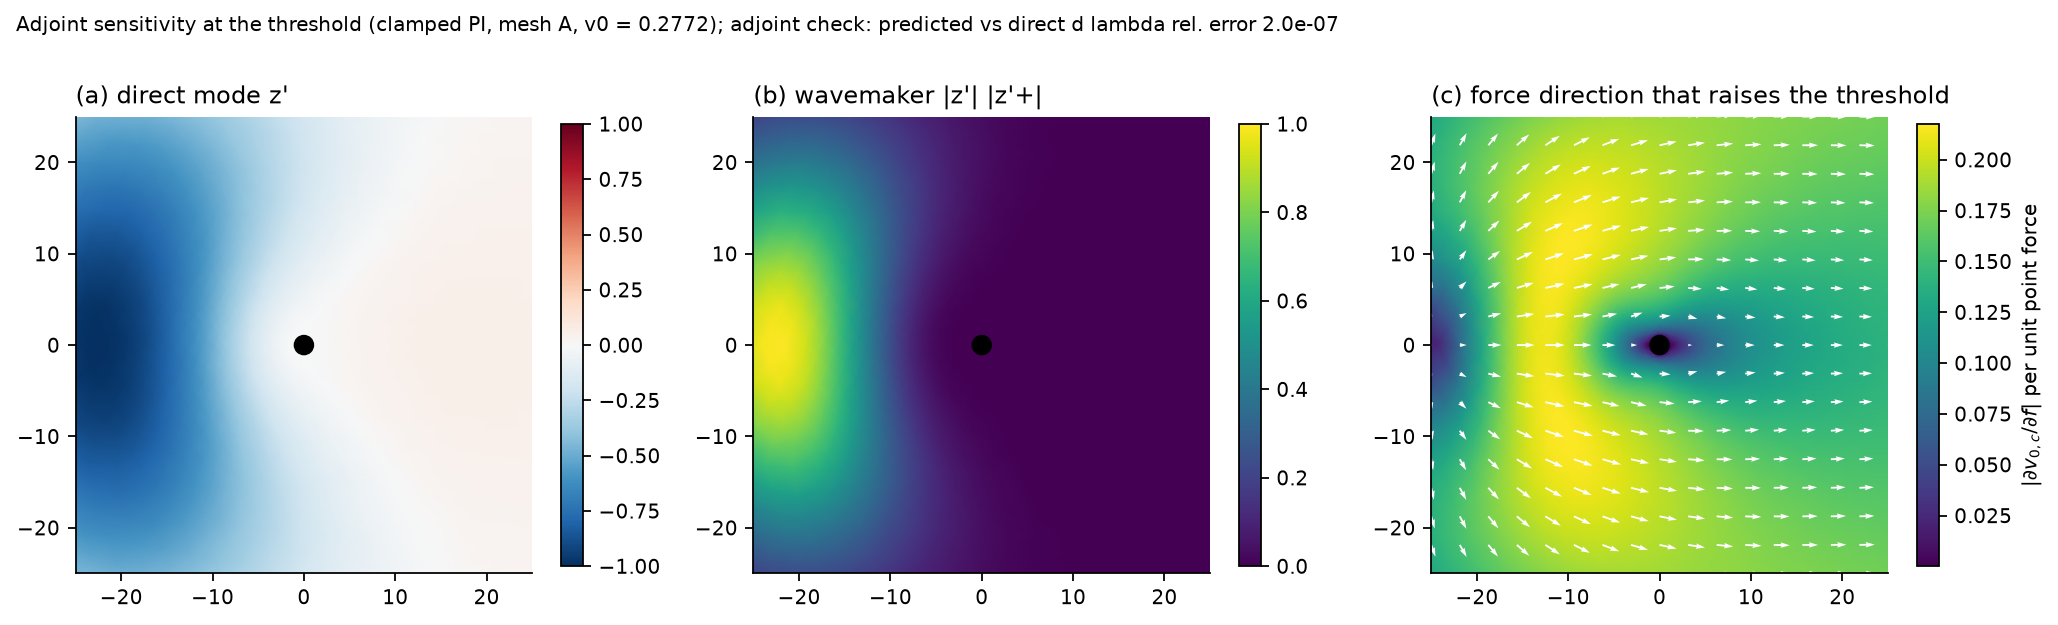
\includegraphics[width=\linewidth,height=86mm,keepaspectratio]{figures/membrane_flow2_sensitivity.png}\captionof{figure}[Archived figure]{Normal direct/adjoint shape, wavemaker, and tangential-force direction that increases the reference threshold. The strong response is located upstream of the inclusion. \textit{Source:} \path{Ruben/membrane_stability/figures/flow2_sensitivity.png}. First added 2026-09-30.}\end{center}
\begin{center}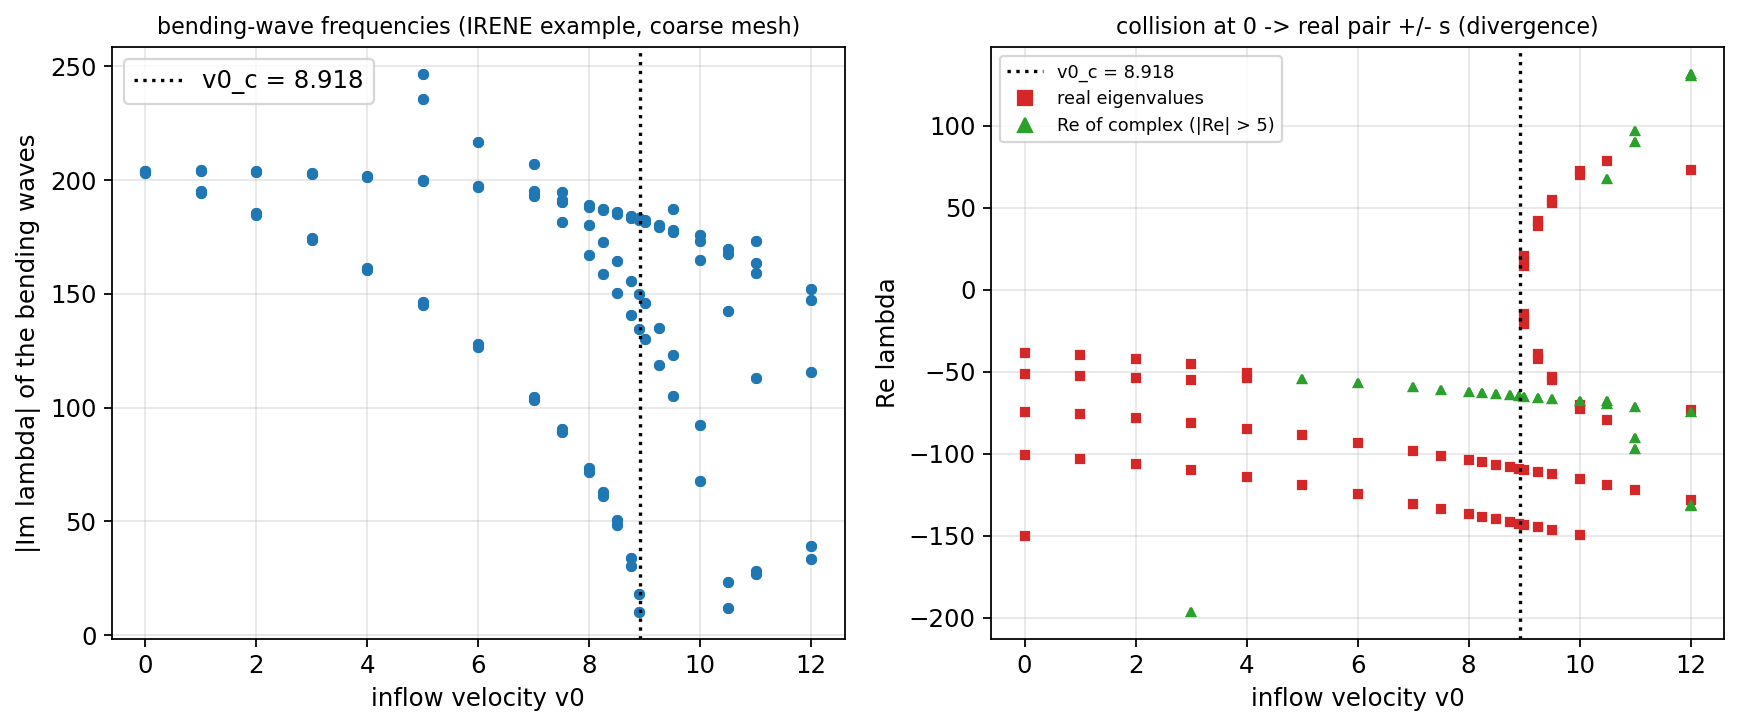
\includegraphics[width=\linewidth,height=86mm,keepaspectratio]{figures/membrane_flow_irene_example_collision.png}\captionof{figure}[Archived figure]{Inertial bending-wave collision in the slip-inclusion example. This is an illustrative high-inertia mechanism, not the overdamped lipid-membrane threshold. \textit{Source:} \path{Ruben/membrane_stability/figures/flow_irene_example_collision.png}. First added 2026-09-30.}\end{center}
\clearpage
\begin{center}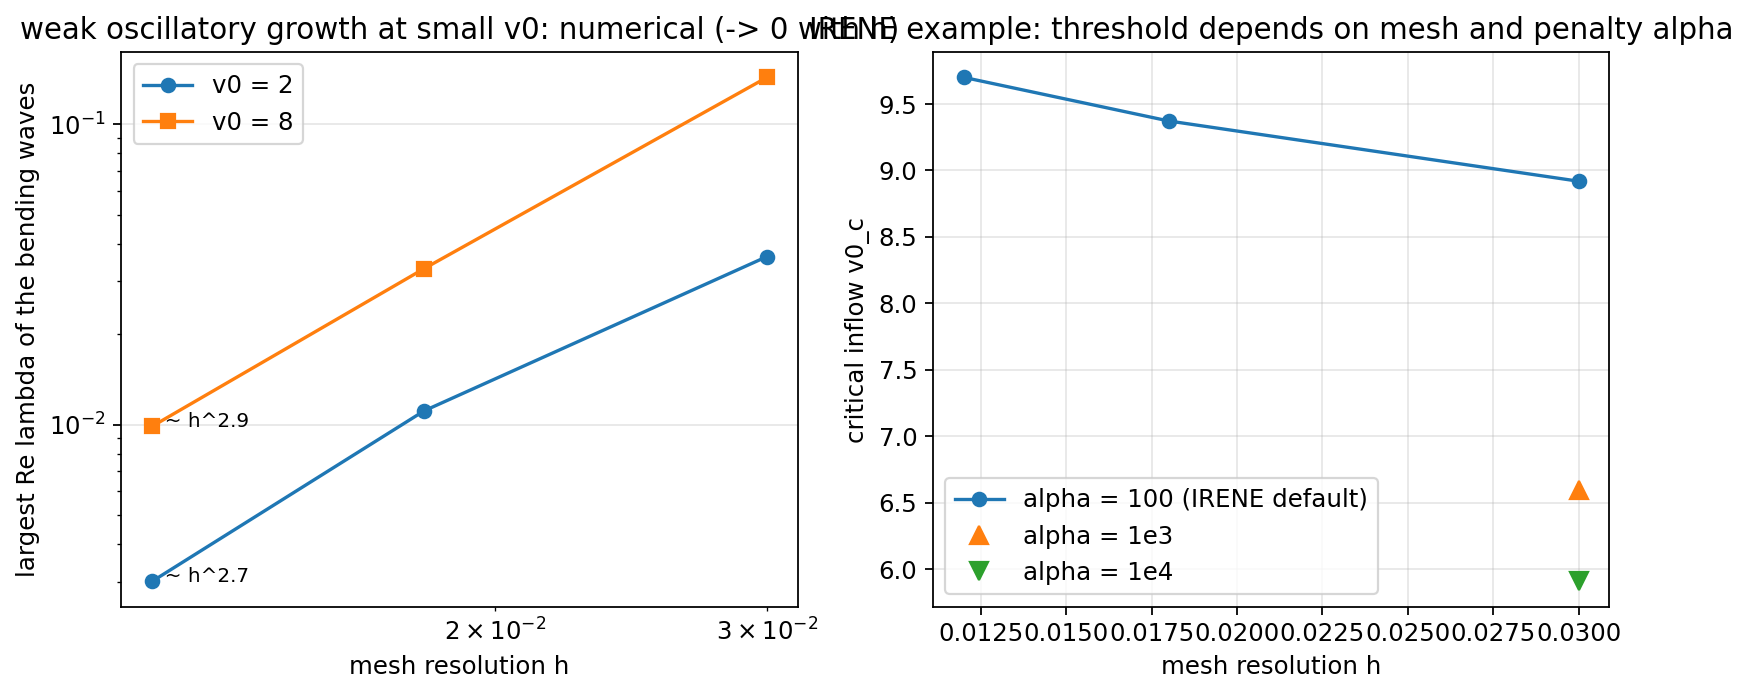
\includegraphics[width=\linewidth,height=182mm,keepaspectratio]{figures/membrane_flow_irene_example_convergence.png}\captionof{figure}[Archived figure]{Slip-penalty example: weak oscillatory growth shrinks with mesh size, while the apparent threshold depends strongly on penalty strength. These results diagnose numerical and boundary-condition sensitivity and are excluded from quantitative core claims. \textit{Source:} \path{Ruben/membrane_stability/figures/flow_irene_example_convergence.png}. First added 2026-09-30.}\end{center}
\clearpage
\begin{center}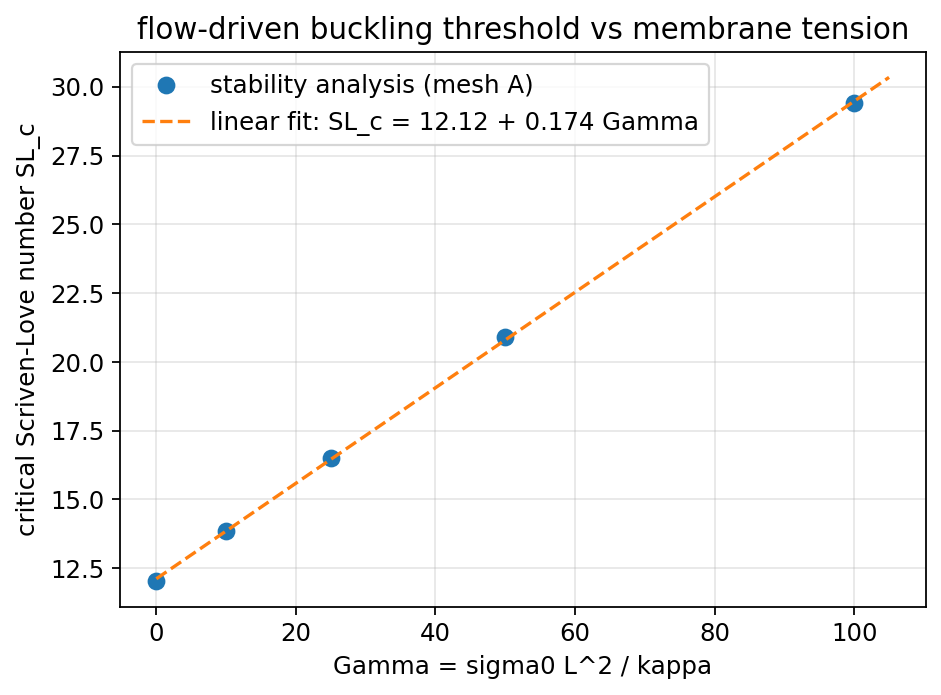
\includegraphics[width=\linewidth,height=182mm,keepaspectratio]{figures/membrane_flow_pre_SLc_vs_tension.png}\captionof{figure}[Archived figure]{Superseded original-rim calculation. Its approximate linear threshold-versus-tension fit belongs to the implementation without vertical protein force balance and must not be used for the corrected physical model. \textit{Source:} \path{Ruben/membrane_stability/figures/flow_pre_SLc_vs_tension.png}. First added 2026-09-30.}\end{center}
\clearpage
\begin{center}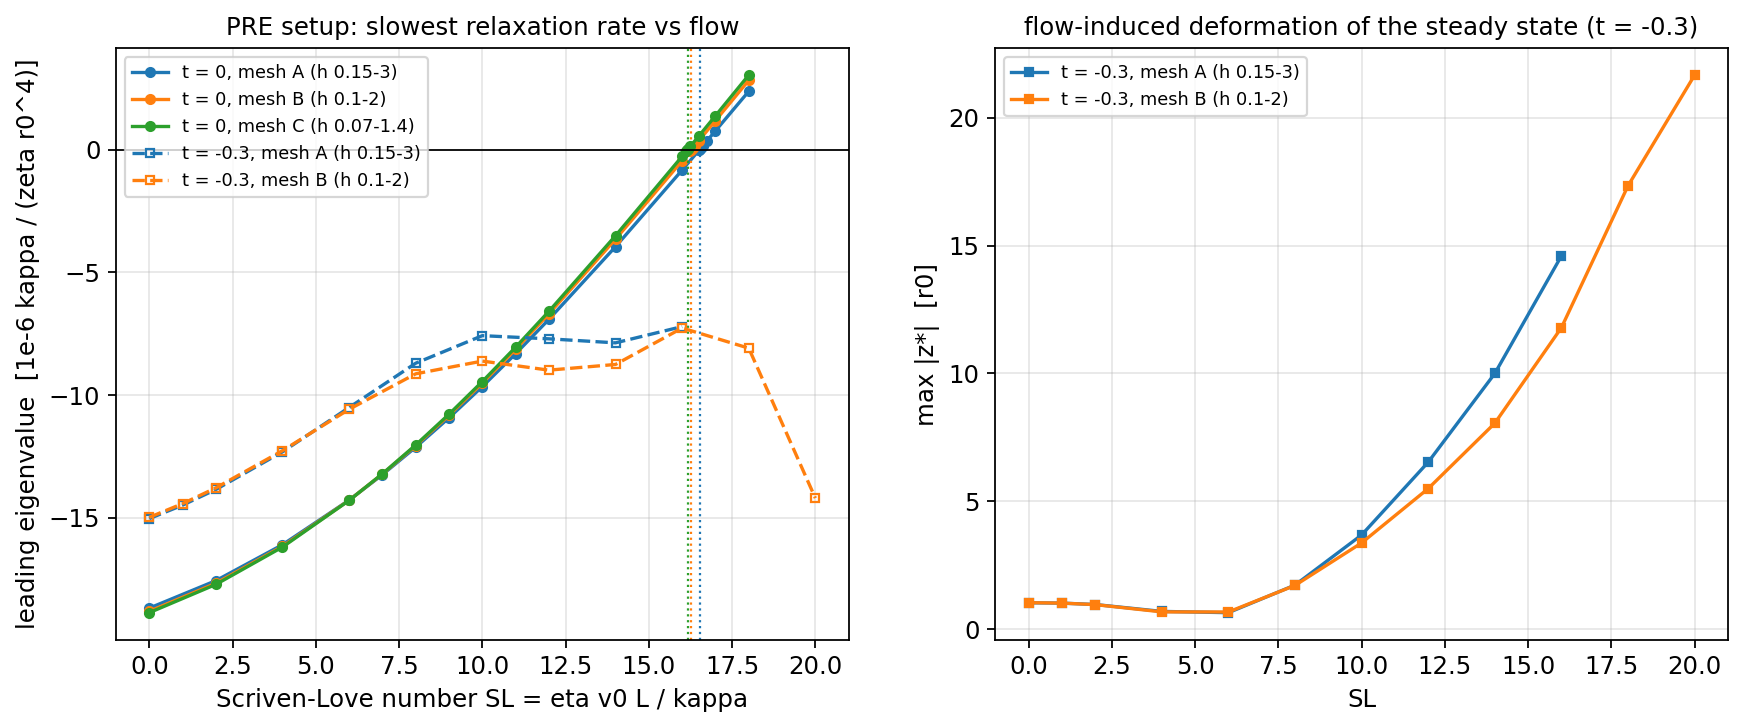
\includegraphics[width=\linewidth,height=86mm,keepaspectratio]{figures/membrane_flow_pre_eigenvalue_vs_SL.png}\captionof{figure}[Archived figure]{Superseded original-rim flow spectra and large imperfect deformation. The roughly sixteen threshold is a diagnostic of the original boundary-value problem; corrected thresholds are near twenty-seven in the reference geometry. \textit{Source:} \path{Ruben/membrane_stability/figures/flow_pre_eigenvalue_vs_SL.png}. First added 2026-09-30.}\end{center}
\begin{center}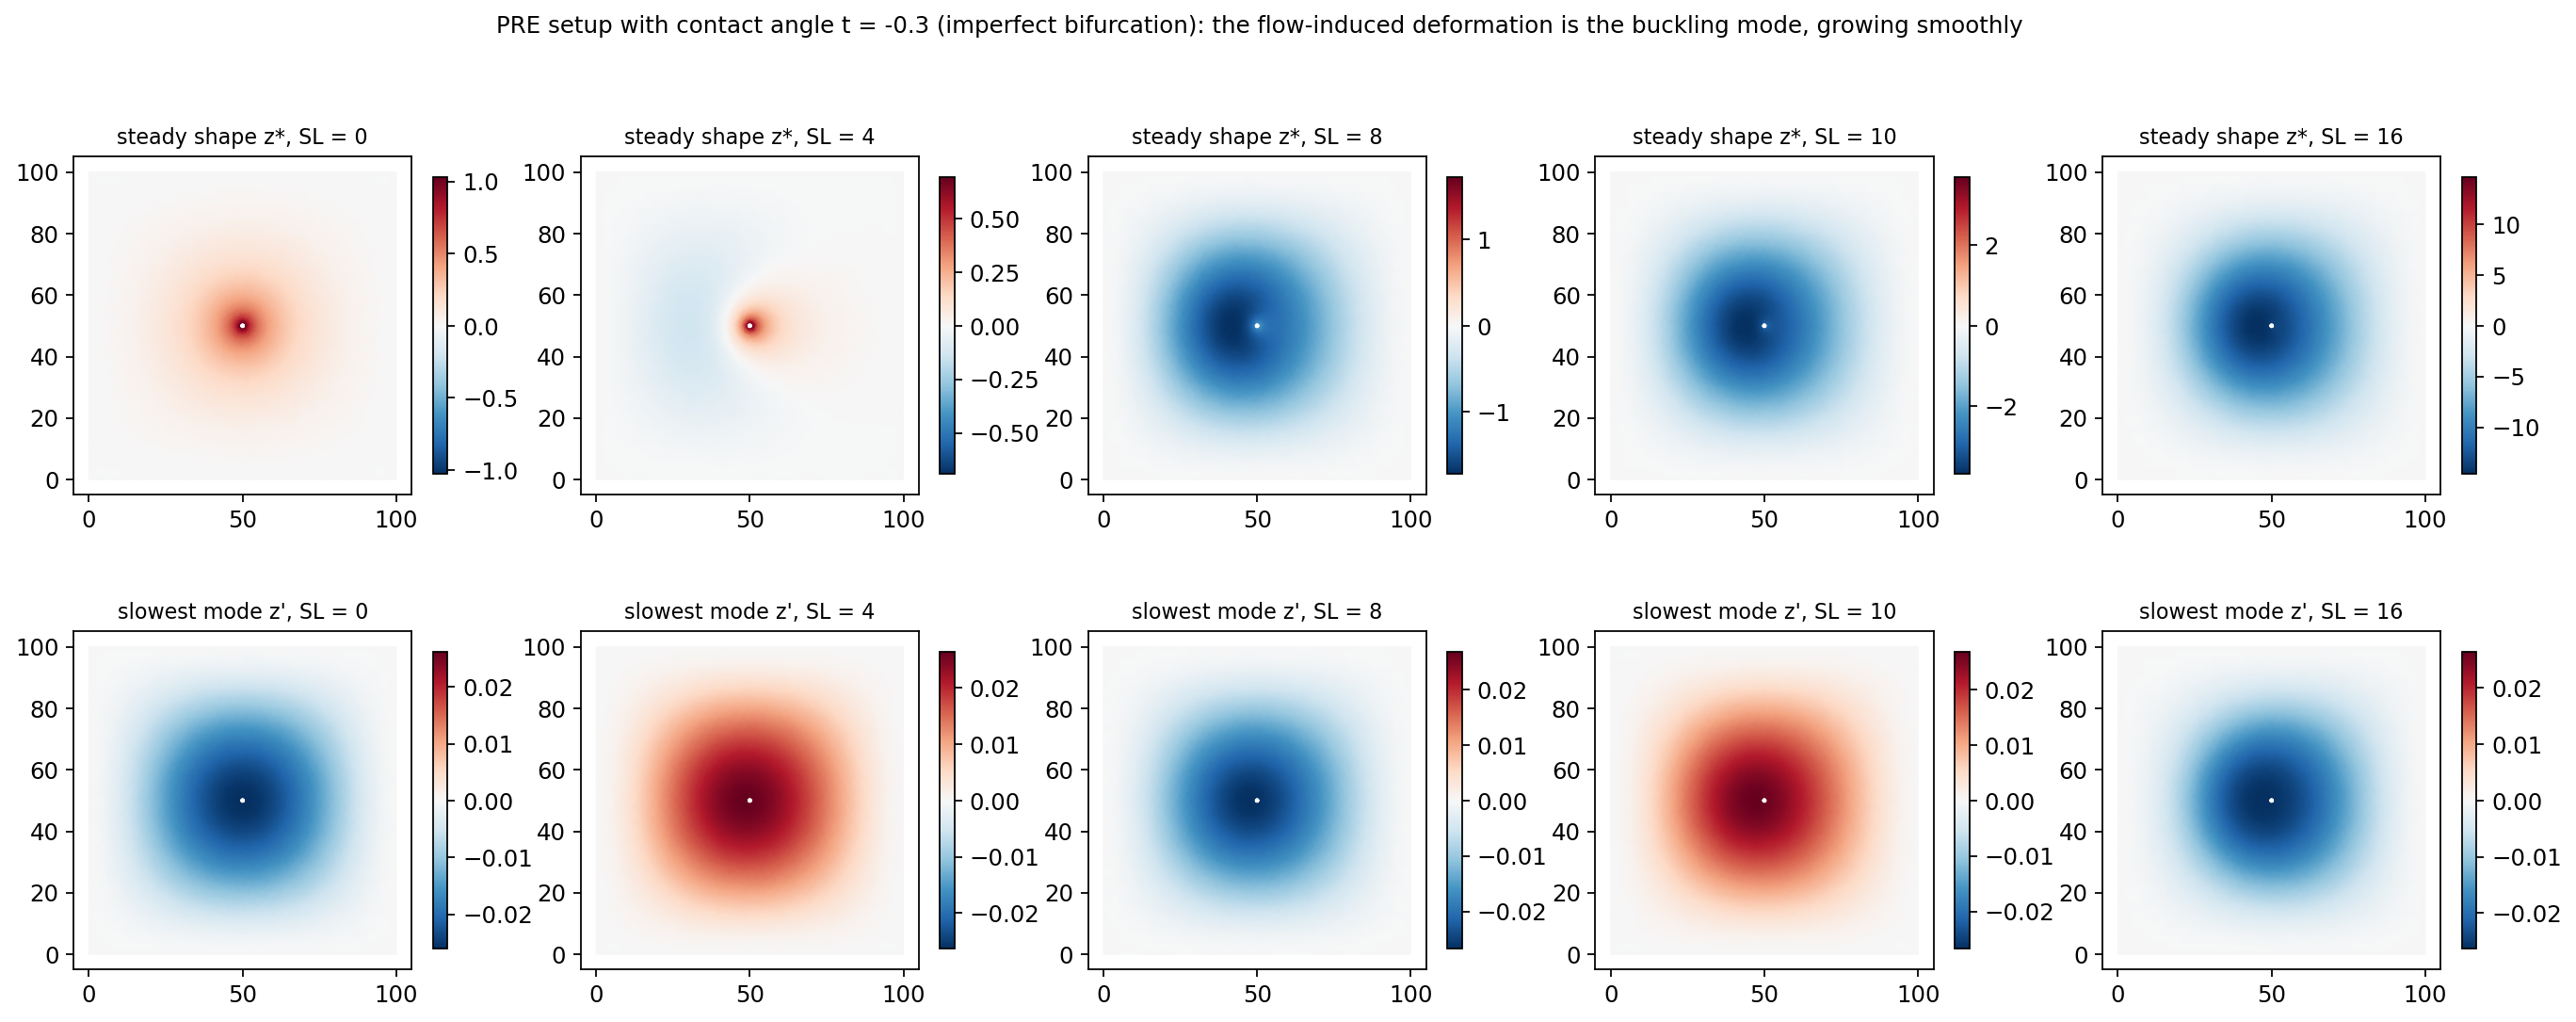
\includegraphics[width=\linewidth,height=86mm,keepaspectratio]{figures/membrane_flow_pre_imperfect_shapes.png}\captionof{figure}[Archived figure]{Superseded original-rim shapes and leading modes at nonzero contact slope. Their large smooth deformation is not evidence for a smooth transition with a physically force-free protein. \textit{Source:} \path{Ruben/membrane_stability/figures/flow_pre_imperfect_shapes.png}. First added 2026-09-30.}\end{center}
\clearpage
\begin{center}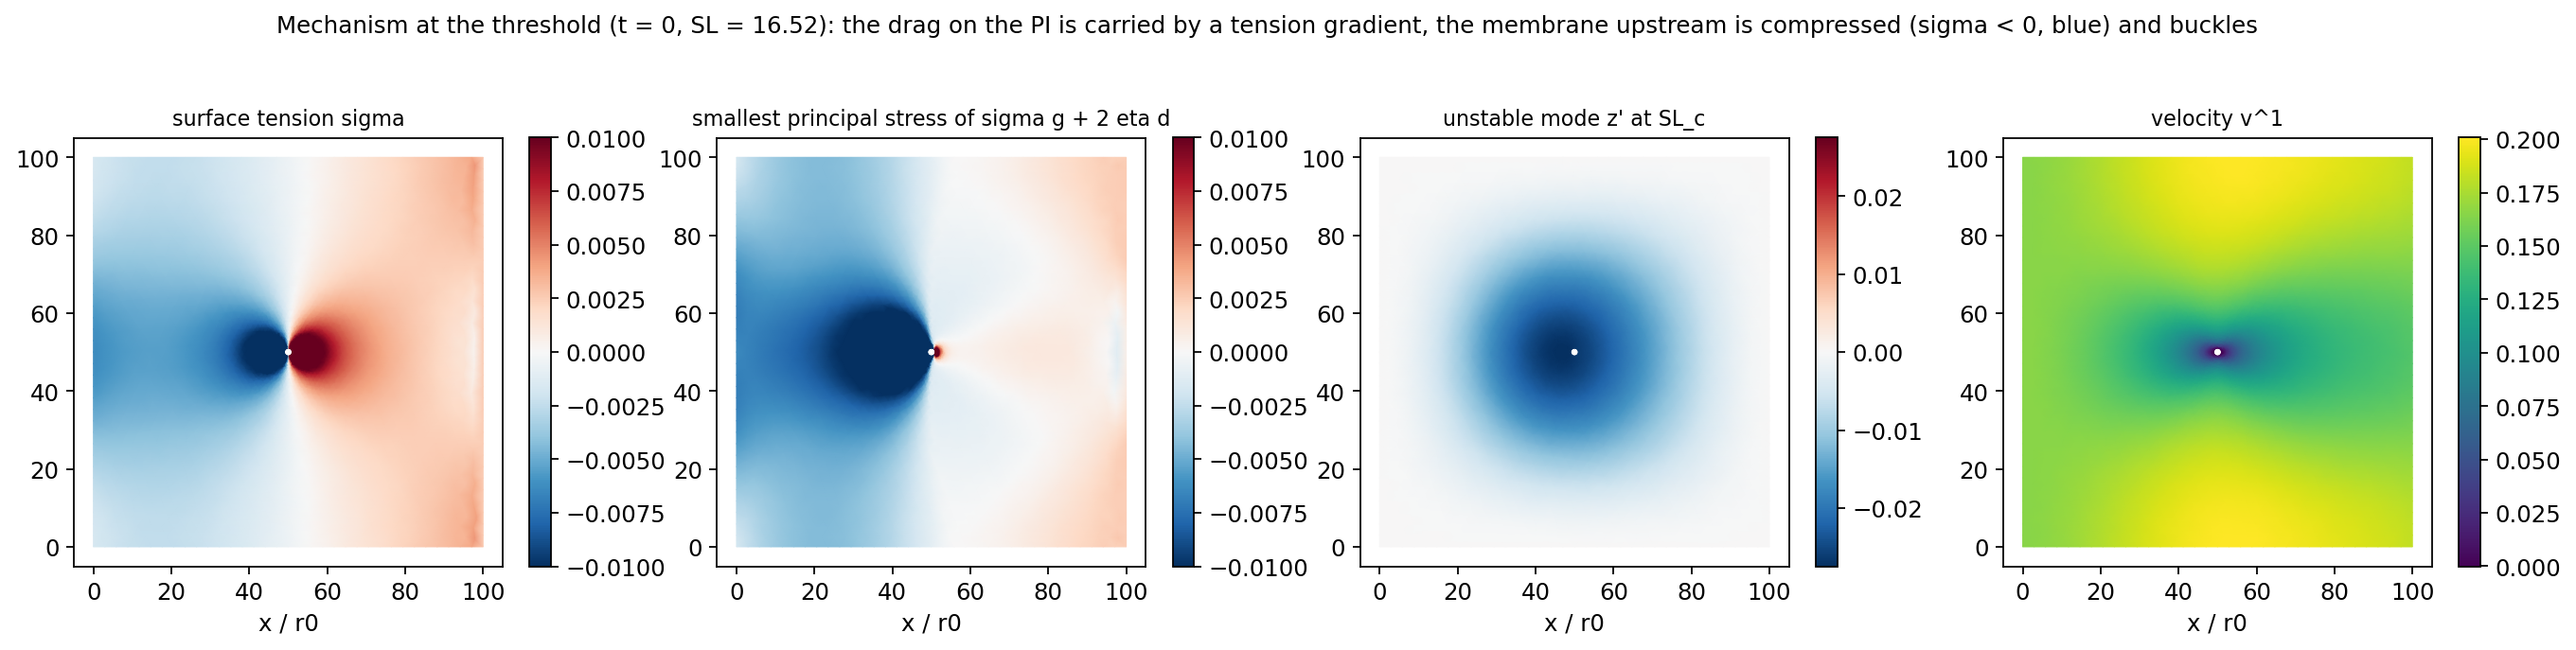
\includegraphics[width=\linewidth,height=86mm,keepaspectratio]{figures/membrane_flow_pre_mechanism.png}\captionof{figure}[Archived figure]{Superseded original-rim stress and eigenmode fields. They reveal upstream compression but place the mode nearer the protein than the corrected force-balanced problem. \textit{Source:} \path{Ruben/membrane_stability/figures/flow_pre_mechanism.png}. First added 2026-09-30.}\end{center}
\begin{center}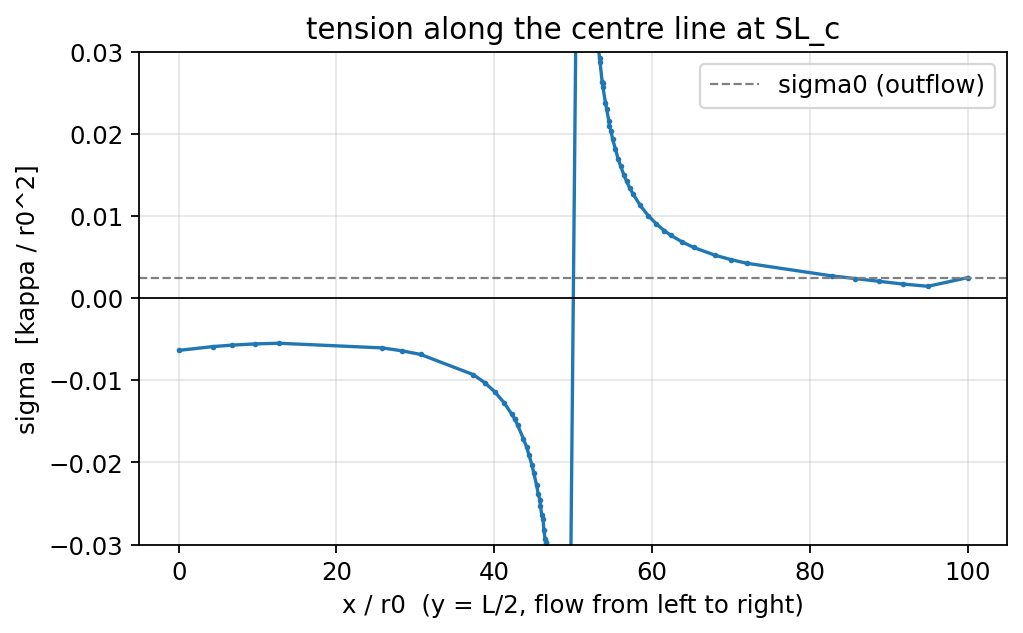
\includegraphics[width=\linewidth,height=86mm,keepaspectratio]{figures/membrane_flow_pre_tension_centreline.png}\captionof{figure}[Archived figure]{Original-rim flat base-flow tension along the centreline. The upstream tension decrease is mechanistic evidence; the onset value attached to this figure is superseded by the physical protein condition. \textit{Source:} \path{Ruben/membrane_stability/figures/flow_pre_tension_centreline.png}. First added 2026-09-30.}\end{center}
\clearpage
\begin{center}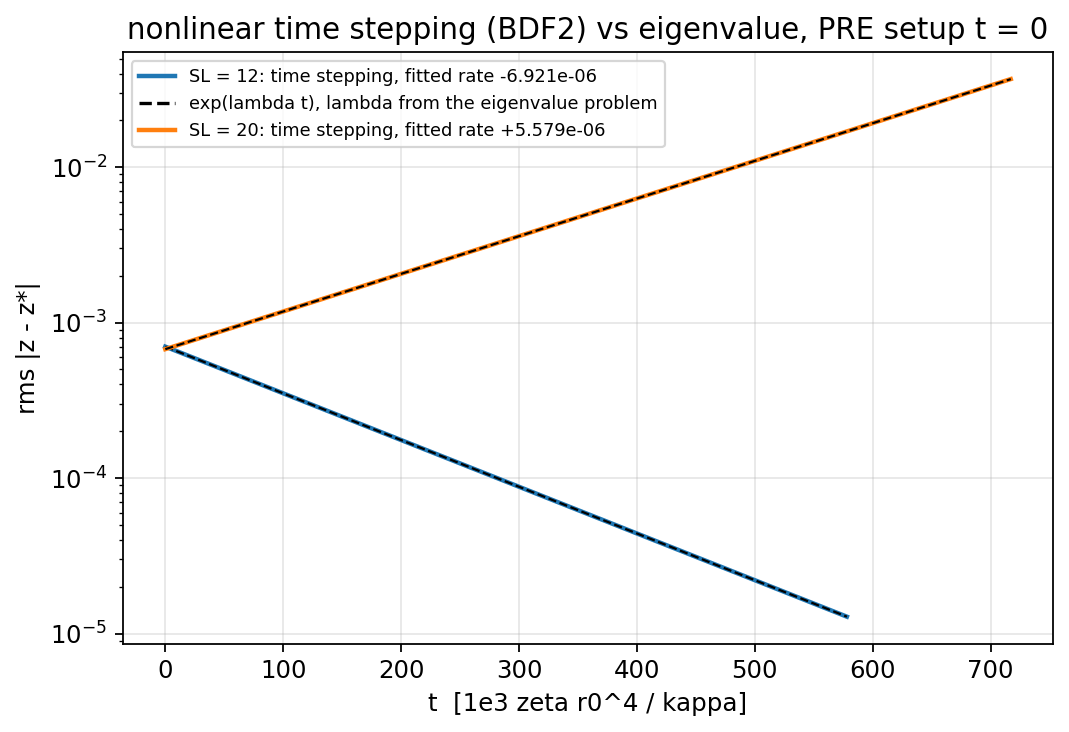
\includegraphics[width=\linewidth,height=182mm,keepaspectratio]{figures/membrane_flow_time_check.png}\captionof{figure}[Archived figure]{BDF2 versus eigenvalue growth and decay for the original-rim implementation. This checks that the numerical linearization predicts that implementation's dynamics, not that its rim condition is physically force-free. \textit{Source:} \path{Ruben/membrane_stability/figures/flow_time_check.png}. First added 2026-09-30.}\end{center}
\clearpage
\begin{center}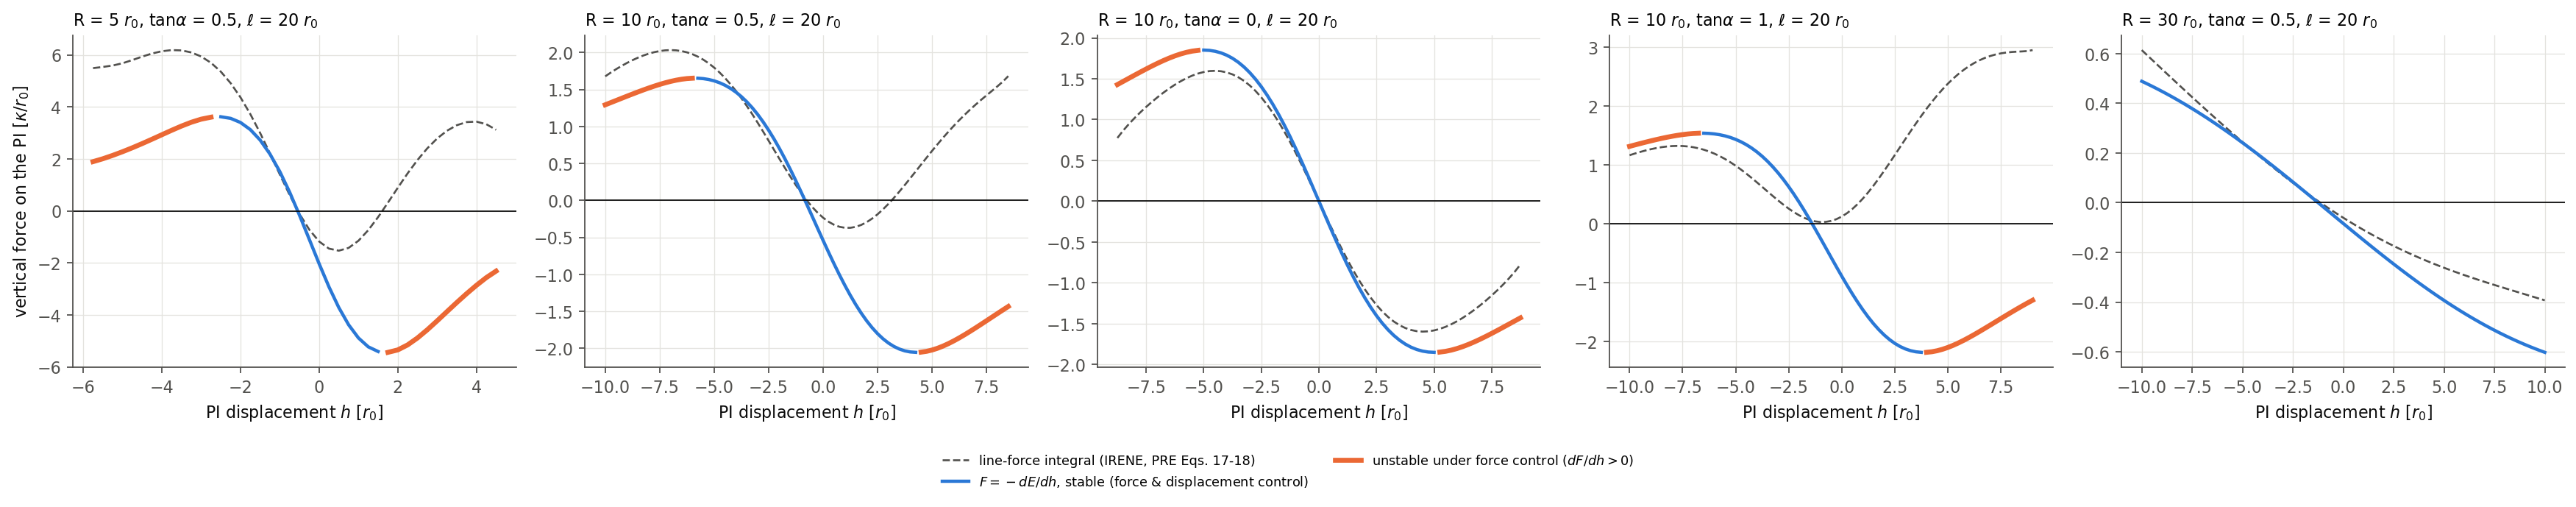
\includegraphics[width=\linewidth,height=86mm,keepaspectratio]{figures/membrane_force_displacement.png}\captionof{figure}[Archived figure]{Ring forces and fixed-height eigenvalues for several radii. Dashed original line-force curves are retained as diagnostics; extrema and force-control conclusions use virtual work. \textit{Source:} \path{Ruben/membrane_stability/figures/force_displacement.png}. First added 2026-09-29.}\end{center}
\begin{center}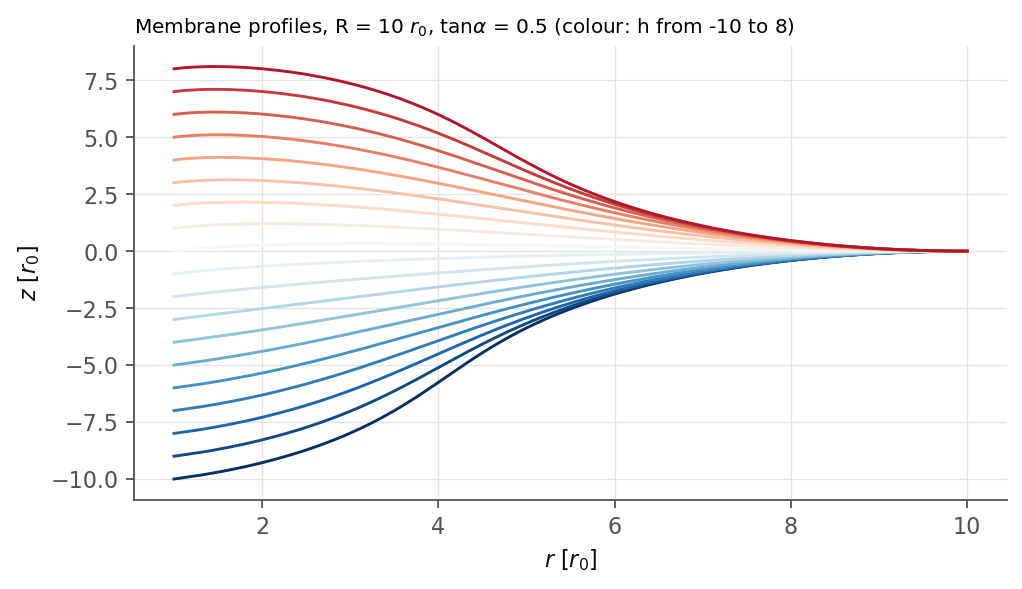
\includegraphics[width=\linewidth,height=86mm,keepaspectratio]{figures/membrane_profiles_ring_R10_tan0.5.png}\captionof{figure}[Archived figure]{Ring profiles for outer radius ten and contact slope one half. Increasing imposed height produces a steep neck while the corresponding fixed-height spectrum remains stable in the sampled range. \textit{Source:} \path{Ruben/membrane_stability/figures/profiles_ring_R10_tan0.5.png}. First added 2026-09-29.}\end{center}
\clearpage
\begin{center}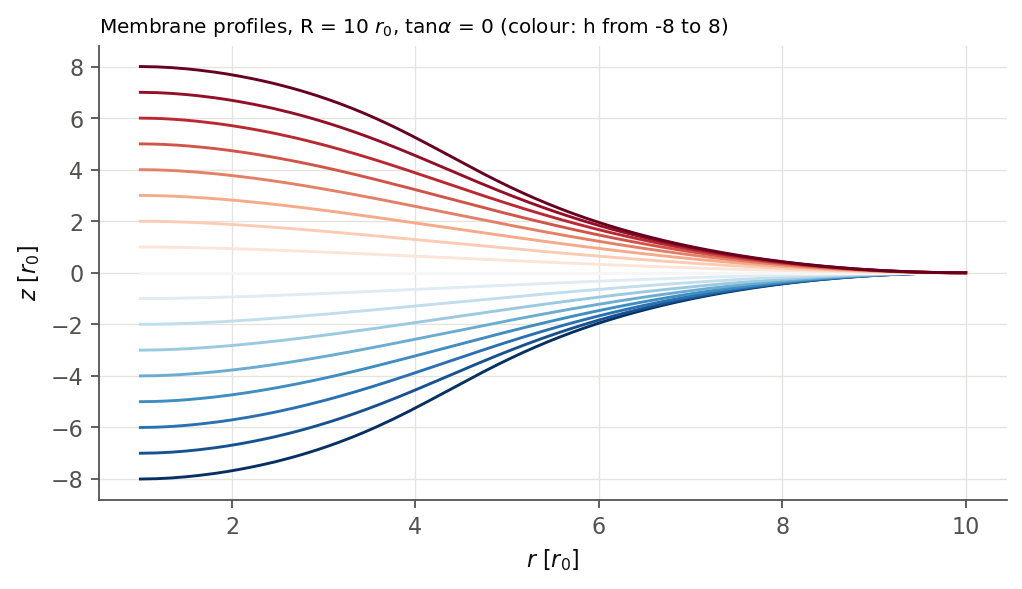
\includegraphics[width=\linewidth,height=182mm,keepaspectratio]{figures/membrane_profiles_ring_R10_tan0.png}\captionof{figure}[Archived figure]{Symmetric zero-contact-slope ring profiles at outer radius ten. Upward and downward branches are related by reflection in the reference plane. \textit{Source:} \path{Ruben/membrane_stability/figures/profiles_ring_R10_tan0.png}. First added 2026-09-29.}\end{center}
\clearpage
\begin{center}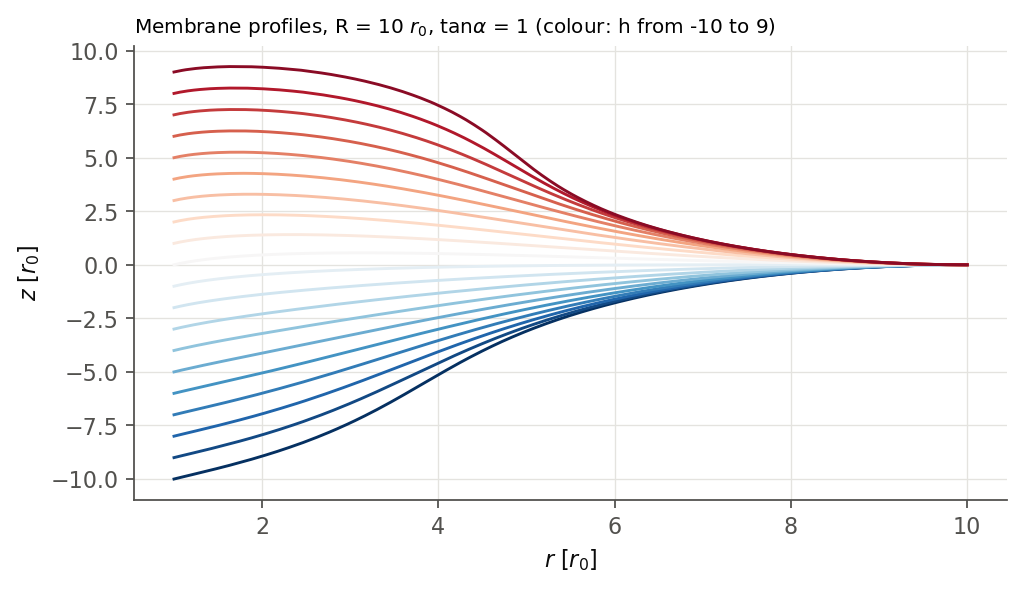
\includegraphics[width=\linewidth,height=182mm,keepaspectratio]{figures/membrane_profiles_ring_R10_tan1.png}\captionof{figure}[Archived figure]{Ring profiles at outer radius ten and unit contact slope. The imposed slope biases the spontaneous height and the two force-control barriers. \textit{Source:} \path{Ruben/membrane_stability/figures/profiles_ring_R10_tan1.png}. First added 2026-09-29.}\end{center}
\clearpage
\begin{center}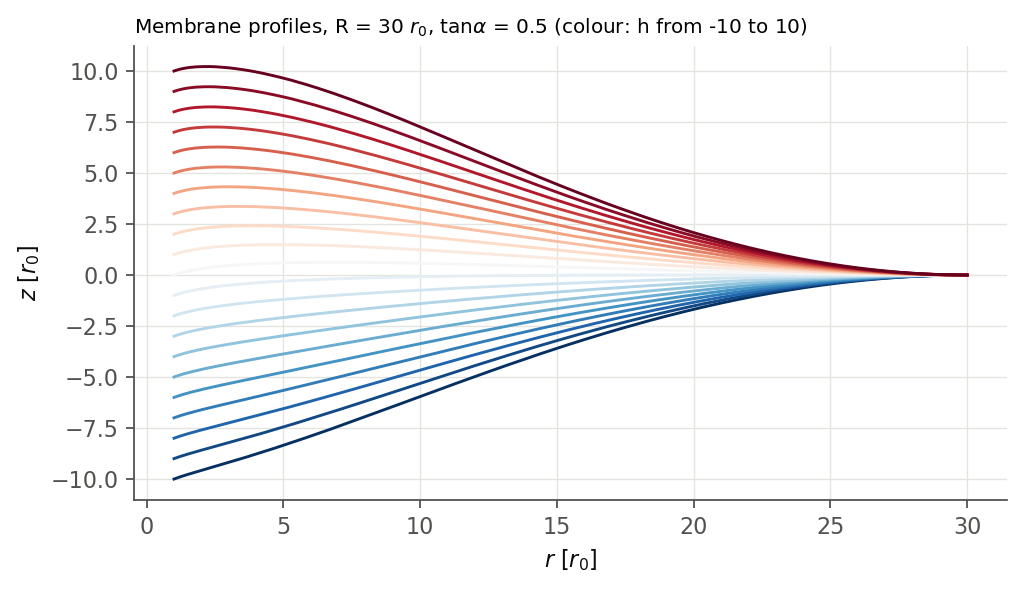
\includegraphics[width=\linewidth,height=182mm,keepaspectratio]{figures/membrane_profiles_ring_R30_tan0.5.png}\captionof{figure}[Archived figure]{Profiles for outer radius thirty and contact slope one half. The displayed Monge window does not reach the long-tube force plateau. \textit{Source:} \path{Ruben/membrane_stability/figures/profiles_ring_R30_tan0.5.png}. First added 2026-09-29.}\end{center}
\clearpage
\begin{center}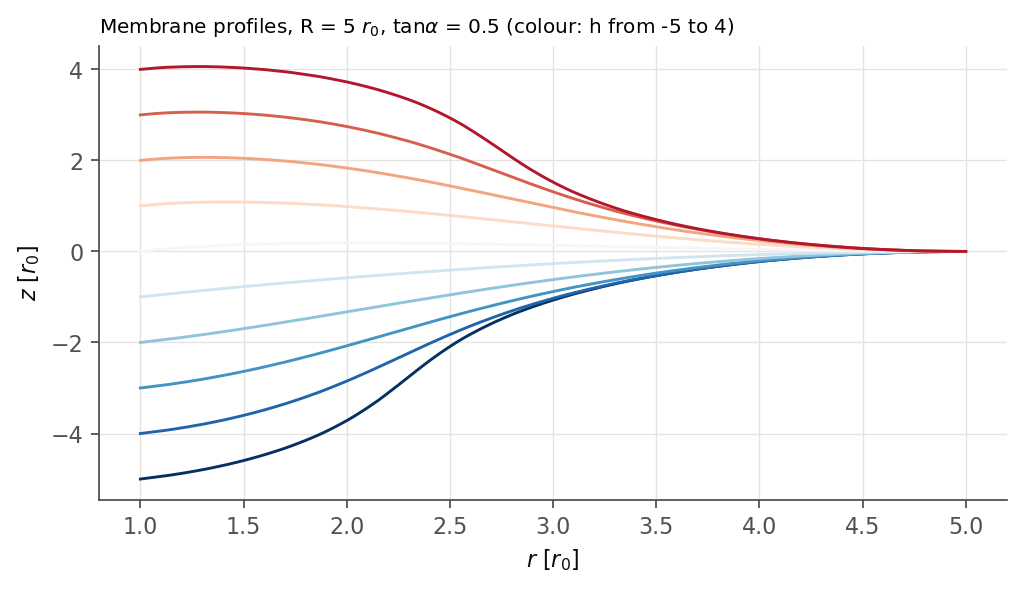
\includegraphics[width=\linewidth,height=86mm,keepaspectratio]{figures/membrane_profiles_ring_R5_tan0.5.png}\captionof{figure}[Archived figure]{Strongly confined ring profiles at outer radius five. Large end slopes limit a height representation and distinguish the confined neck from a freely developed wide tube. \textit{Source:} \path{Ruben/membrane_stability/figures/profiles_ring_R5_tan0.5.png}. First added 2026-09-29.}\end{center}
\begin{center}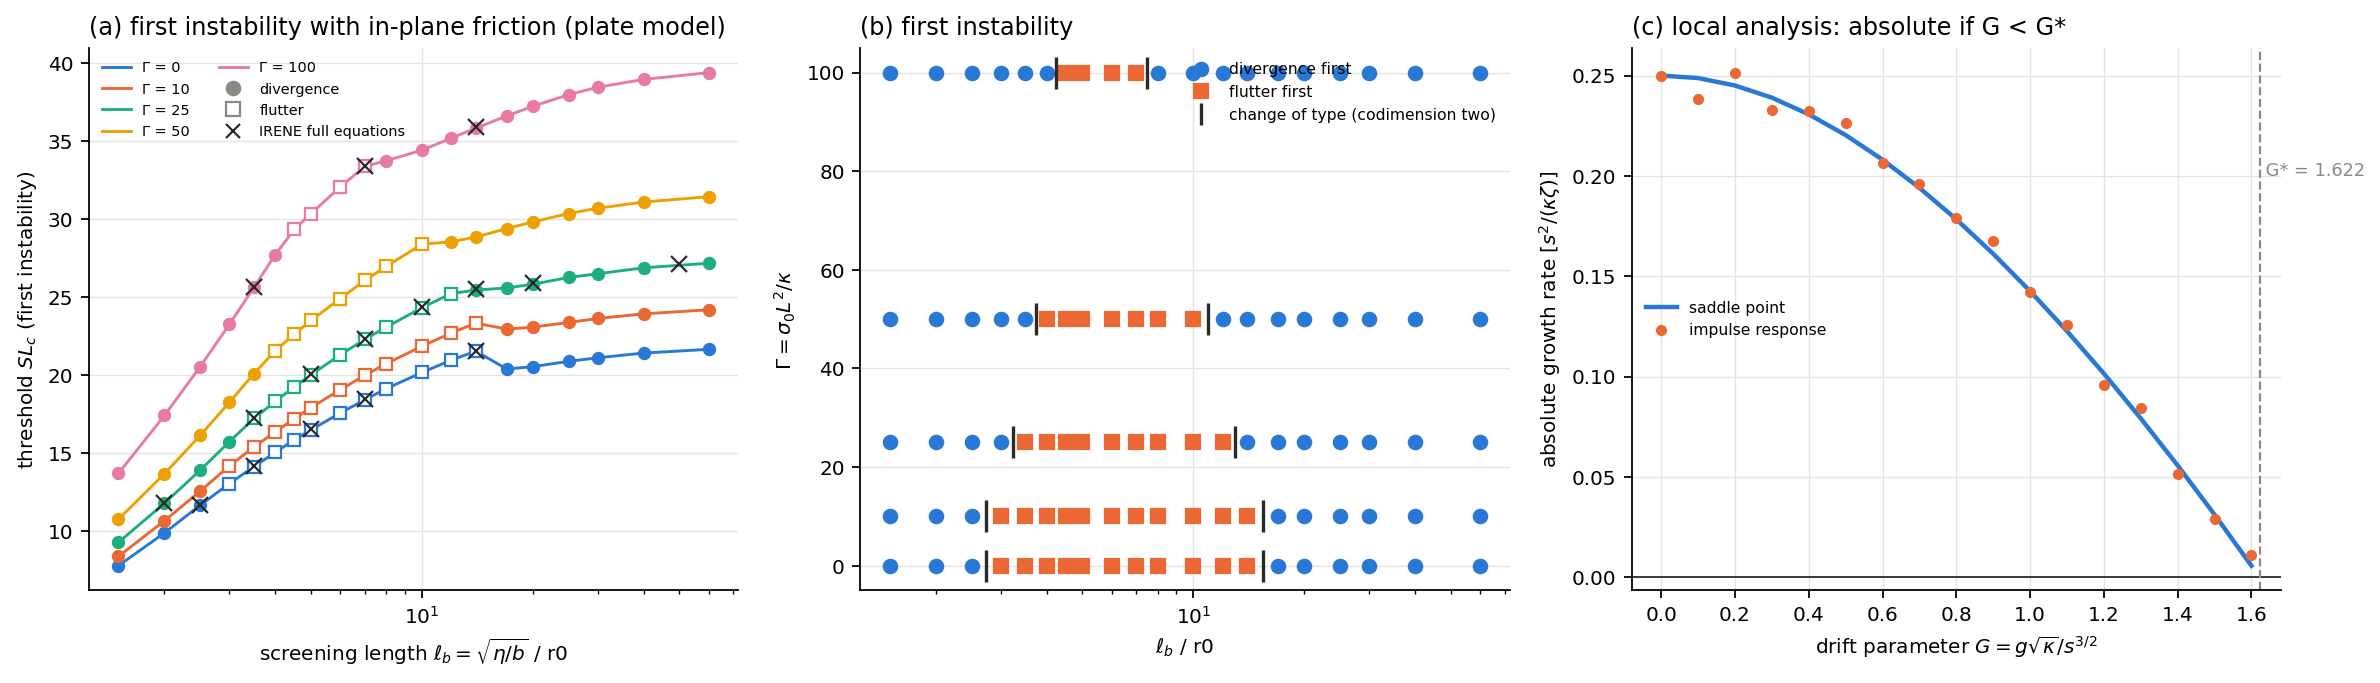
\includegraphics[width=\linewidth,height=86mm,keepaspectratio]{figures/membrane_r3_flutter_map.png}\captionof{figure}[Archived figure]{Divergence/flutter onset map versus screening length and tension, with full-equation checks. The local absolute-instability panel is a guide to the global wave source; near onset the local wavelength is comparable to the compressed region. \textit{Source:} \path{Ruben/membrane_stability/figures/r3_flutter_map.png}. First added 2026-10-01.}\end{center}
\clearpage
\begin{center}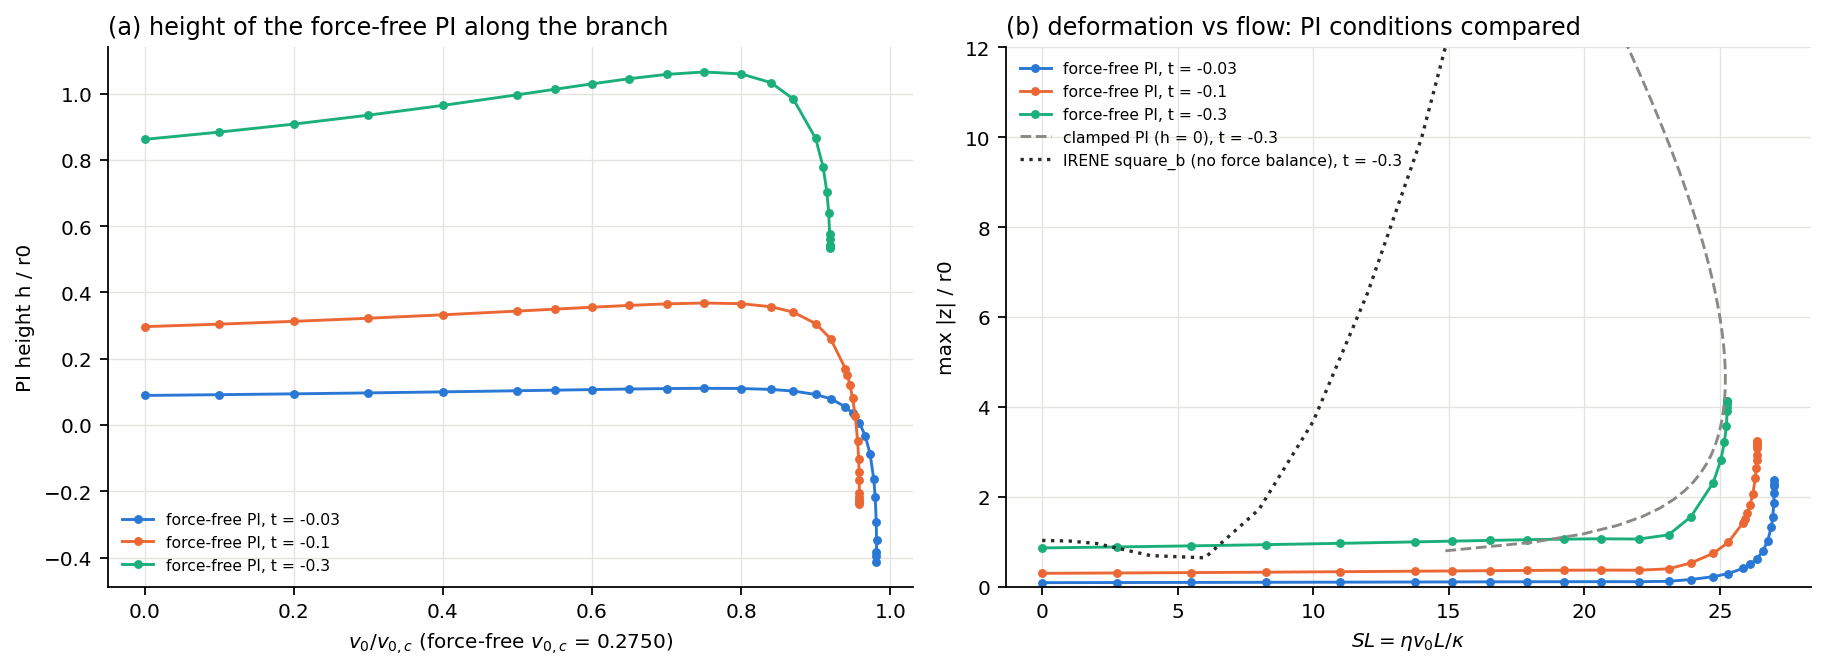
\includegraphics[width=\linewidth,height=182mm,keepaspectratio]{figures/membrane_r3_forcefree.png}\captionof{figure}[Archived figure]{Nonlinear force-free branches for nonzero contact slopes, contrasted with clamped and original-rim conditions. The corrected free protein stays near its rest deformation before an imperfection-sensitive fold. \textit{Source:} \path{Ruben/membrane_stability/figures/r3_forcefree.png}. First added 2026-10-01.}\end{center}
\clearpage
\begin{center}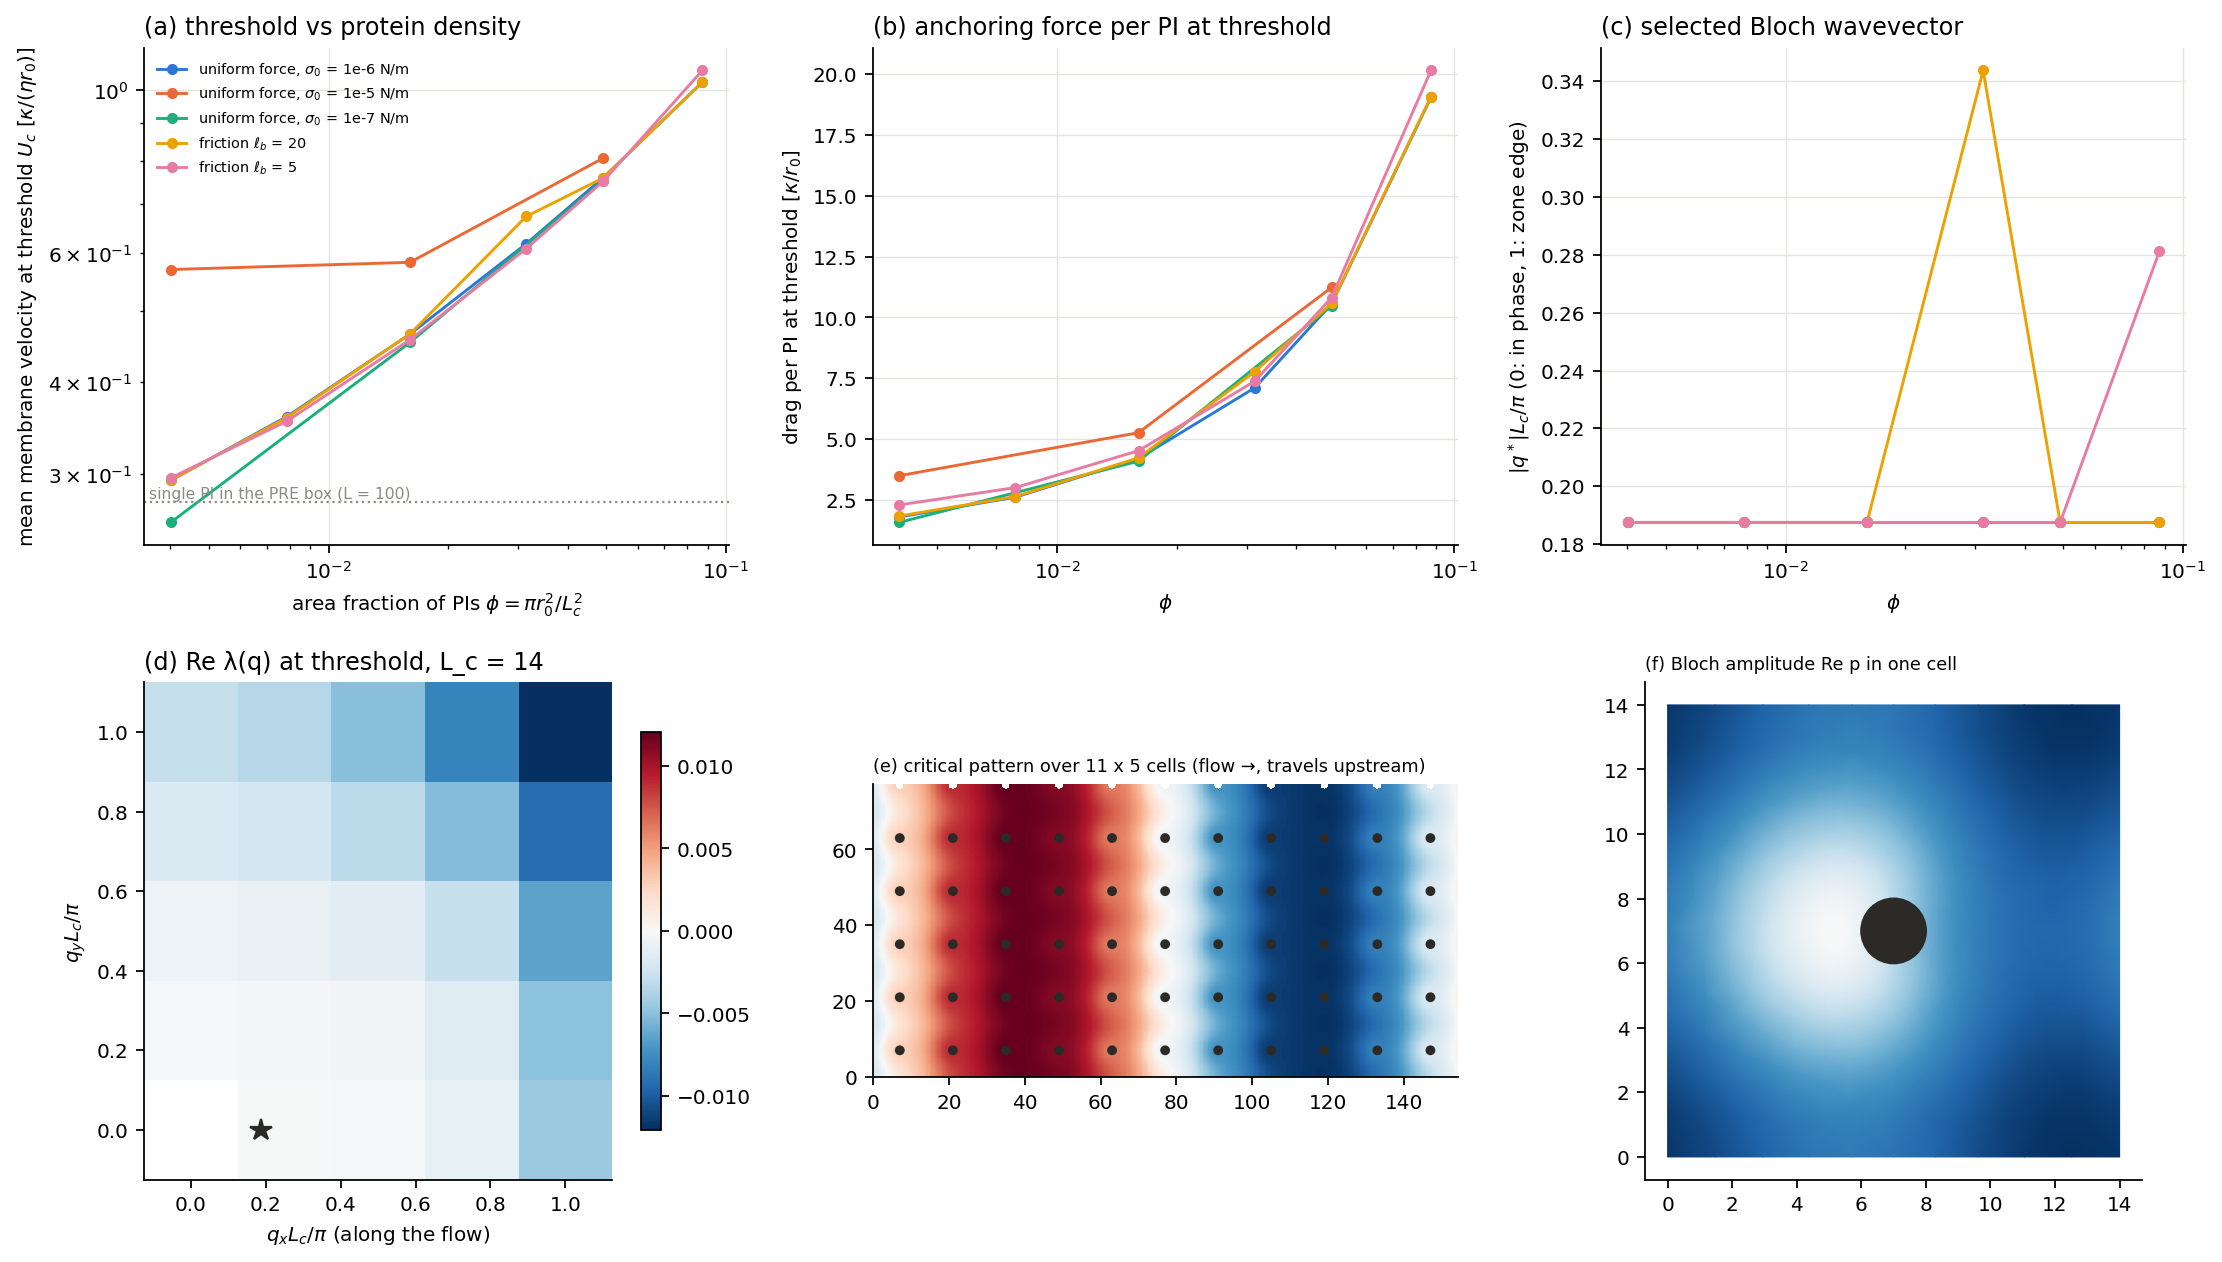
\includegraphics[width=\linewidth,height=182mm,keepaspectratio]{figures/membrane_r3_lattice.png}\captionof{figure}[Archived figure]{Periodic array spectra and patterns. Early finite-wavevector scans are interpreted with the dedicated later long-wave coefficients: a neutral uniform translation exists at zero wavevector, and the longitudinal stiffness controls onset. \textit{Source:} \path{Ruben/membrane_stability/figures/r3_lattice.png}. First added 2026-10-01.}\end{center}
\clearpage
\begin{center}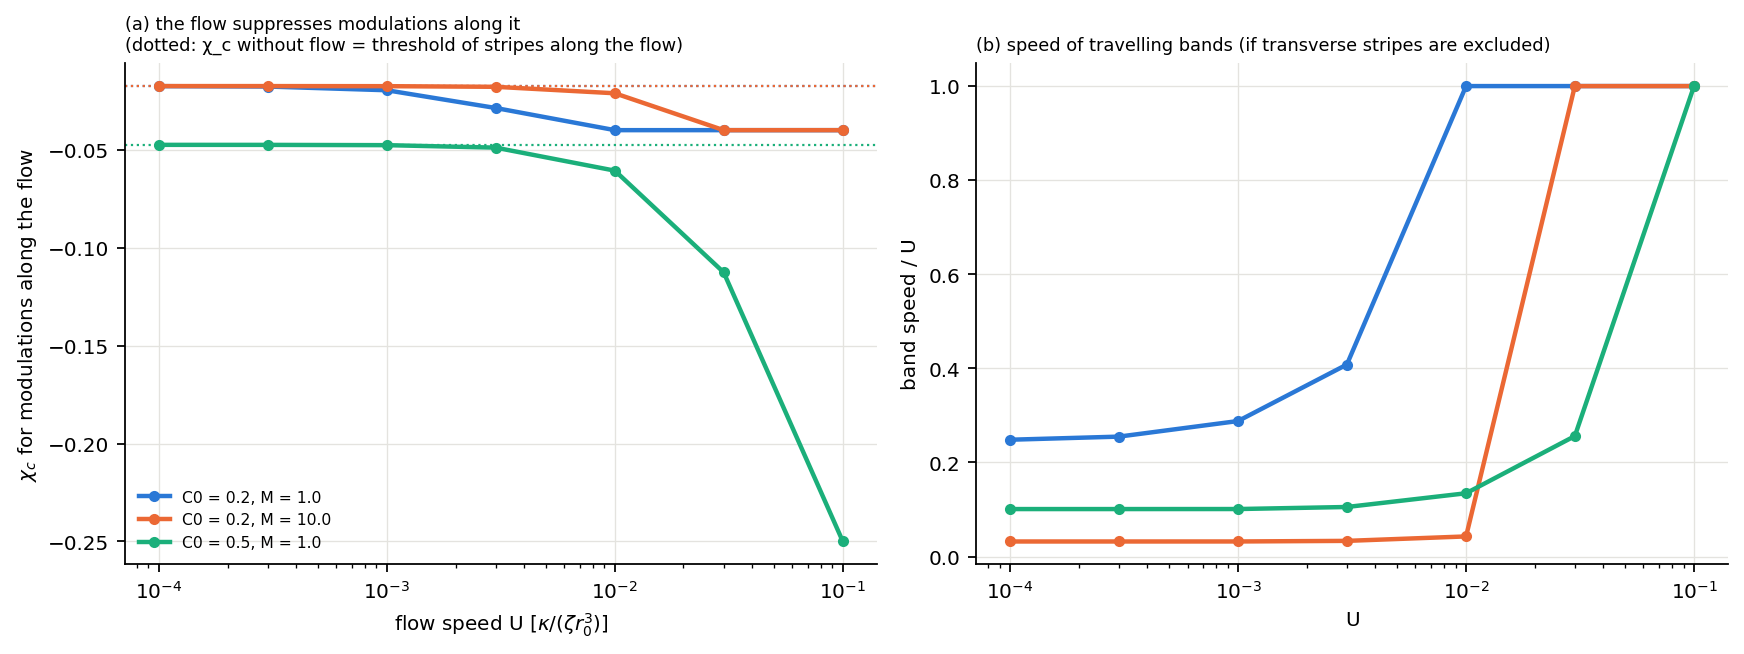
\includegraphics[width=\linewidth,height=182mm,keepaspectratio]{figures/membrane_r3_mobile.png}\captionof{figure}[Archived figure]{Uniform-plane curvature-protein dispersion under relative drift. Transverse wavevectors remain least affected, giving stripes parallel to the flow; travelling longitudinal bands require suppressing those transverse modes. \textit{Source:} \path{Ruben/membrane_stability/figures/r3_mobile.png}. First added 2026-10-01.}\end{center}
\clearpage
\begin{center}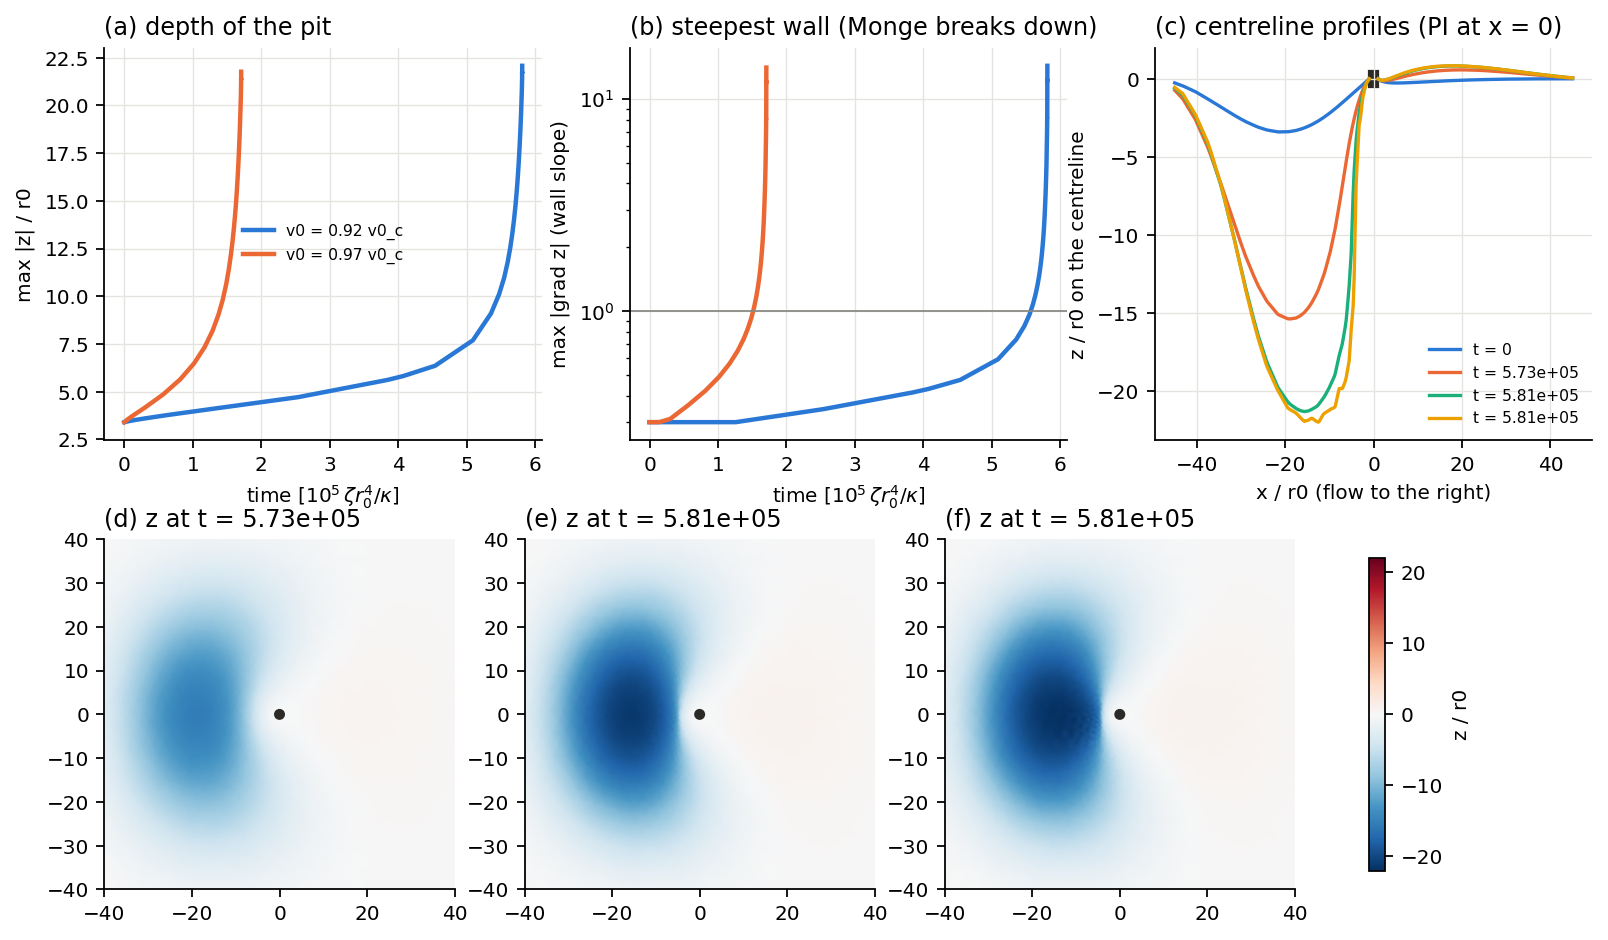
\includegraphics[width=\linewidth,height=182mm,keepaspectratio]{figures/membrane_r3_snap.png}\captionof{figure}[Archived figure]{Clamped-protein time stepping after the fold: bottleneck, deepening upstream pit, and rapid slope growth. The final steep shapes are at the Monge limit, not resolved steady attractors. \textit{Source:} \path{Ruben/membrane_stability/figures/r3_snap.png}. First added 2026-10-01.}\end{center}
\clearpage
\begin{center}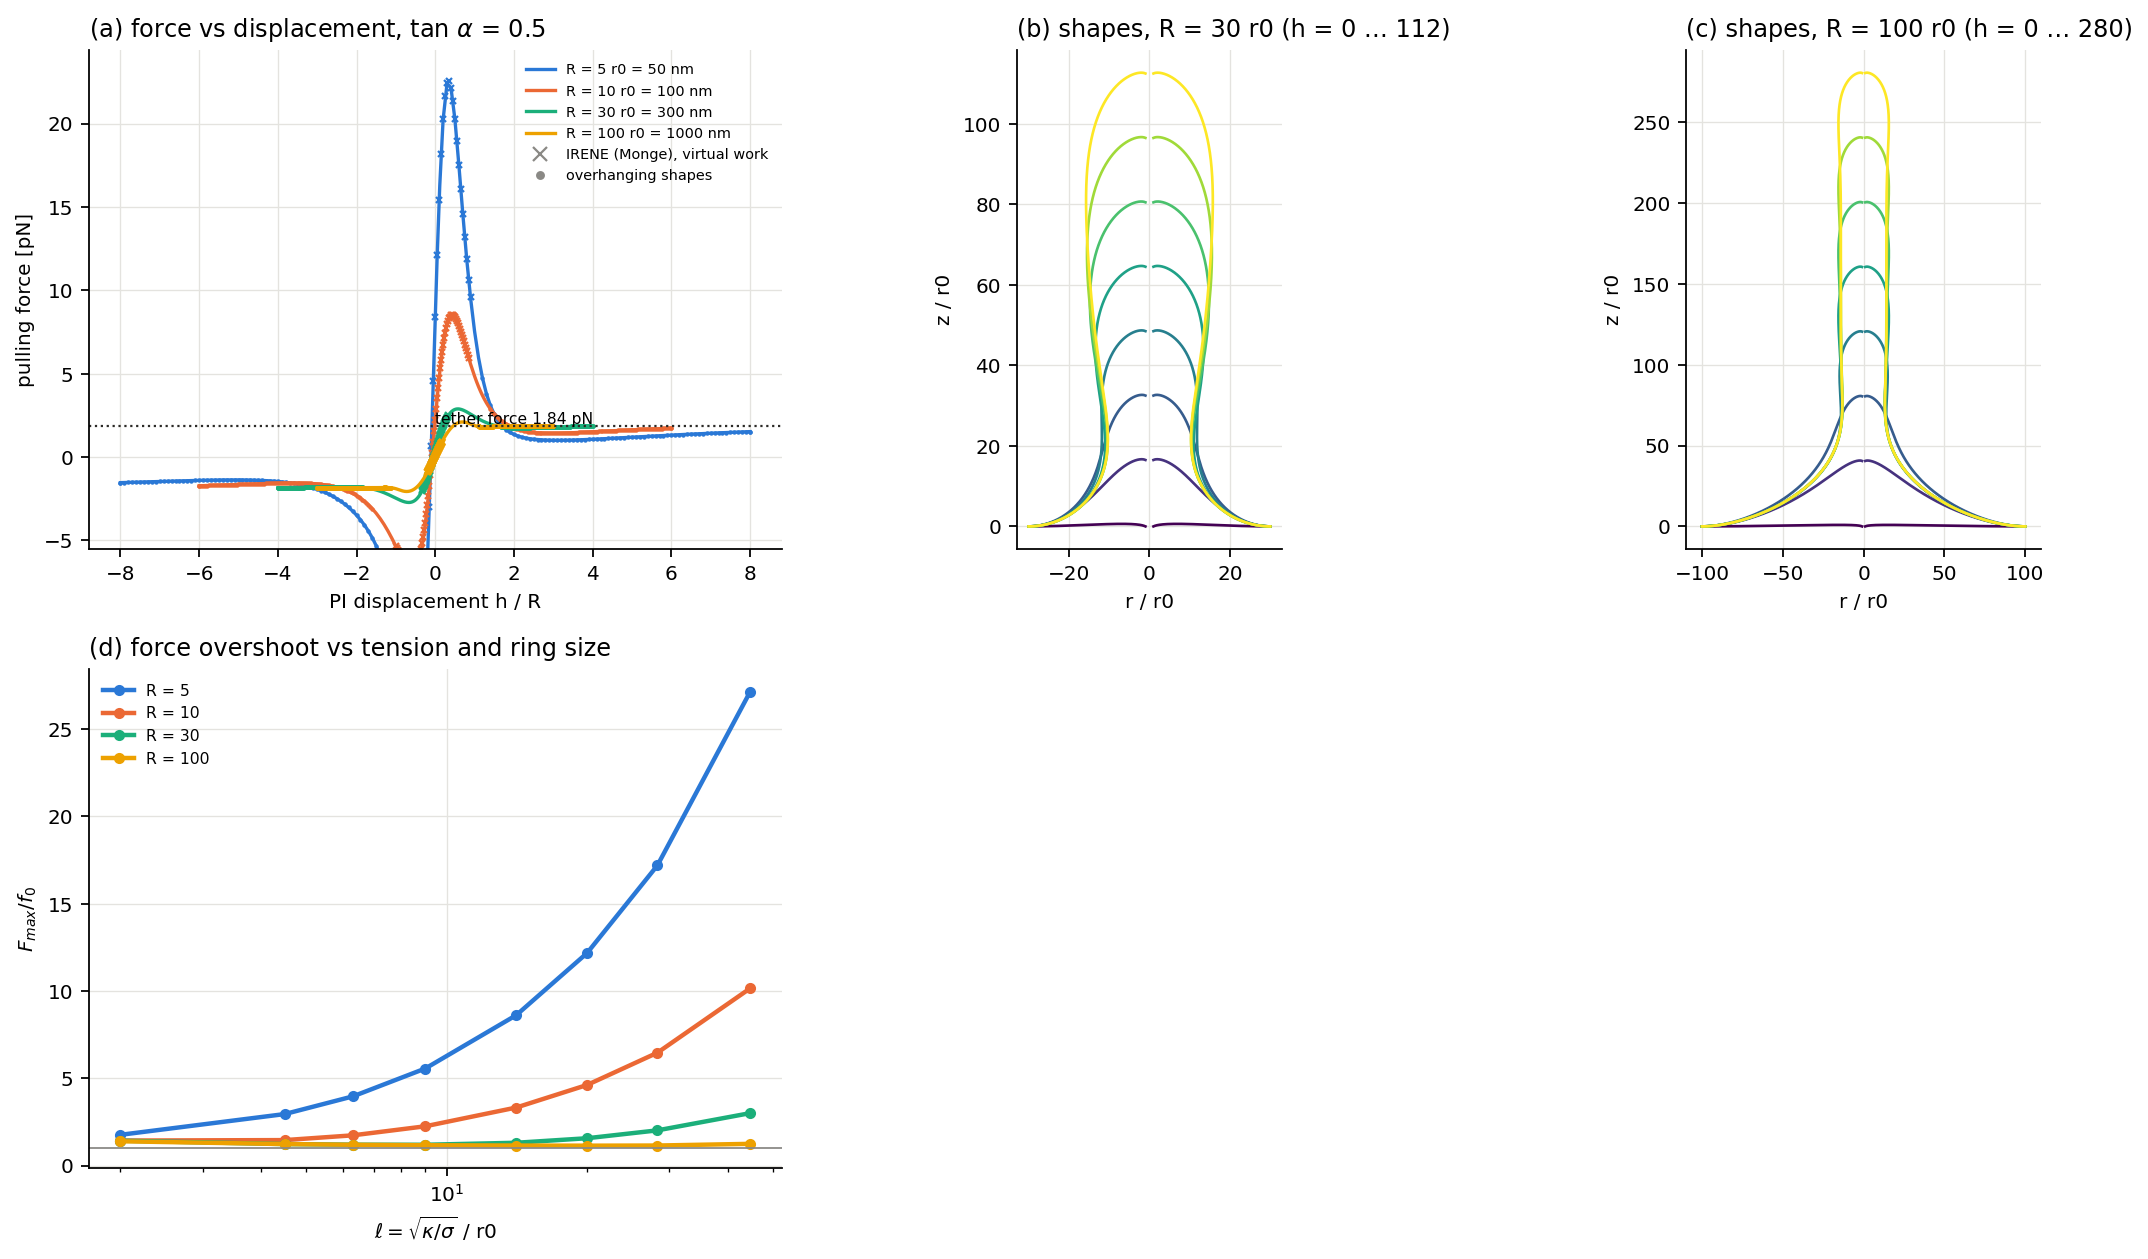
\includegraphics[width=\linewidth,height=182mm,keepaspectratio]{figures/membrane_r3_tube.png}\captionof{figure}[Archived figure]{No-flow axisymmetric arclength continuation. Large rings develop tubes tending to the tether-force plateau; small rings constrain a neck and show a large force overshoot. This is distinct from flow-driven tube growth, which remains unfinished. \textit{Source:} \path{Ruben/membrane_stability/figures/r3_tube.png}. First added 2026-10-01.}\end{center}
\clearpage
\begin{center}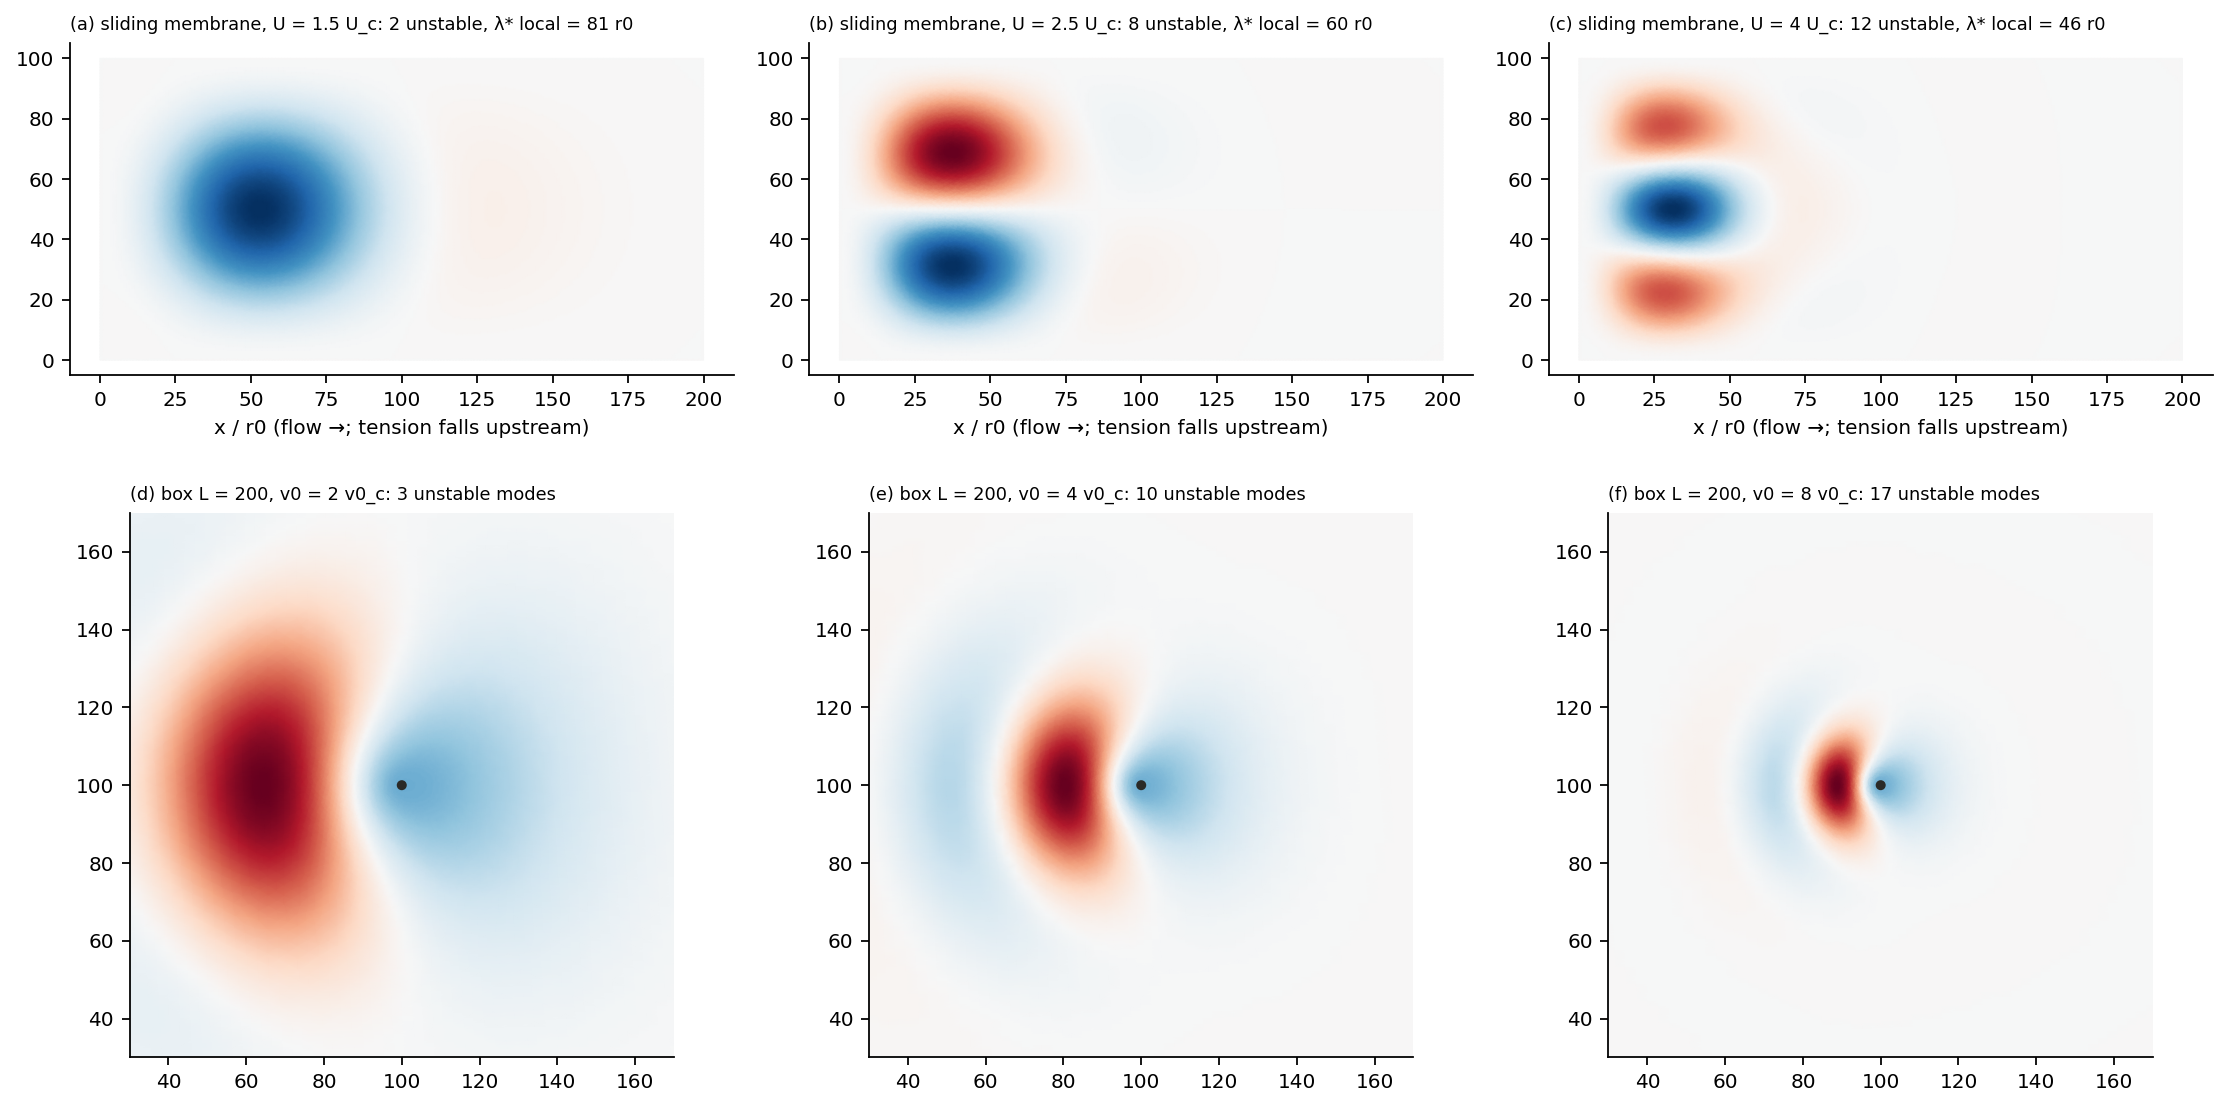
\includegraphics[width=\linewidth,height=86mm,keepaspectratio]{figures/membrane_r3_wrinkles.png}\captionof{figure}[Archived figure]{Plate-model modes well above onset and in sliding-membrane examples. Increasing compression permits multiple lobes and wrinkle trains; these modes do not establish a stable nonlinear pattern around a single protein. \textit{Source:} \path{Ruben/membrane_stability/figures/r3_wrinkles.png}. First added 2026-10-01.}\end{center}
\begin{center}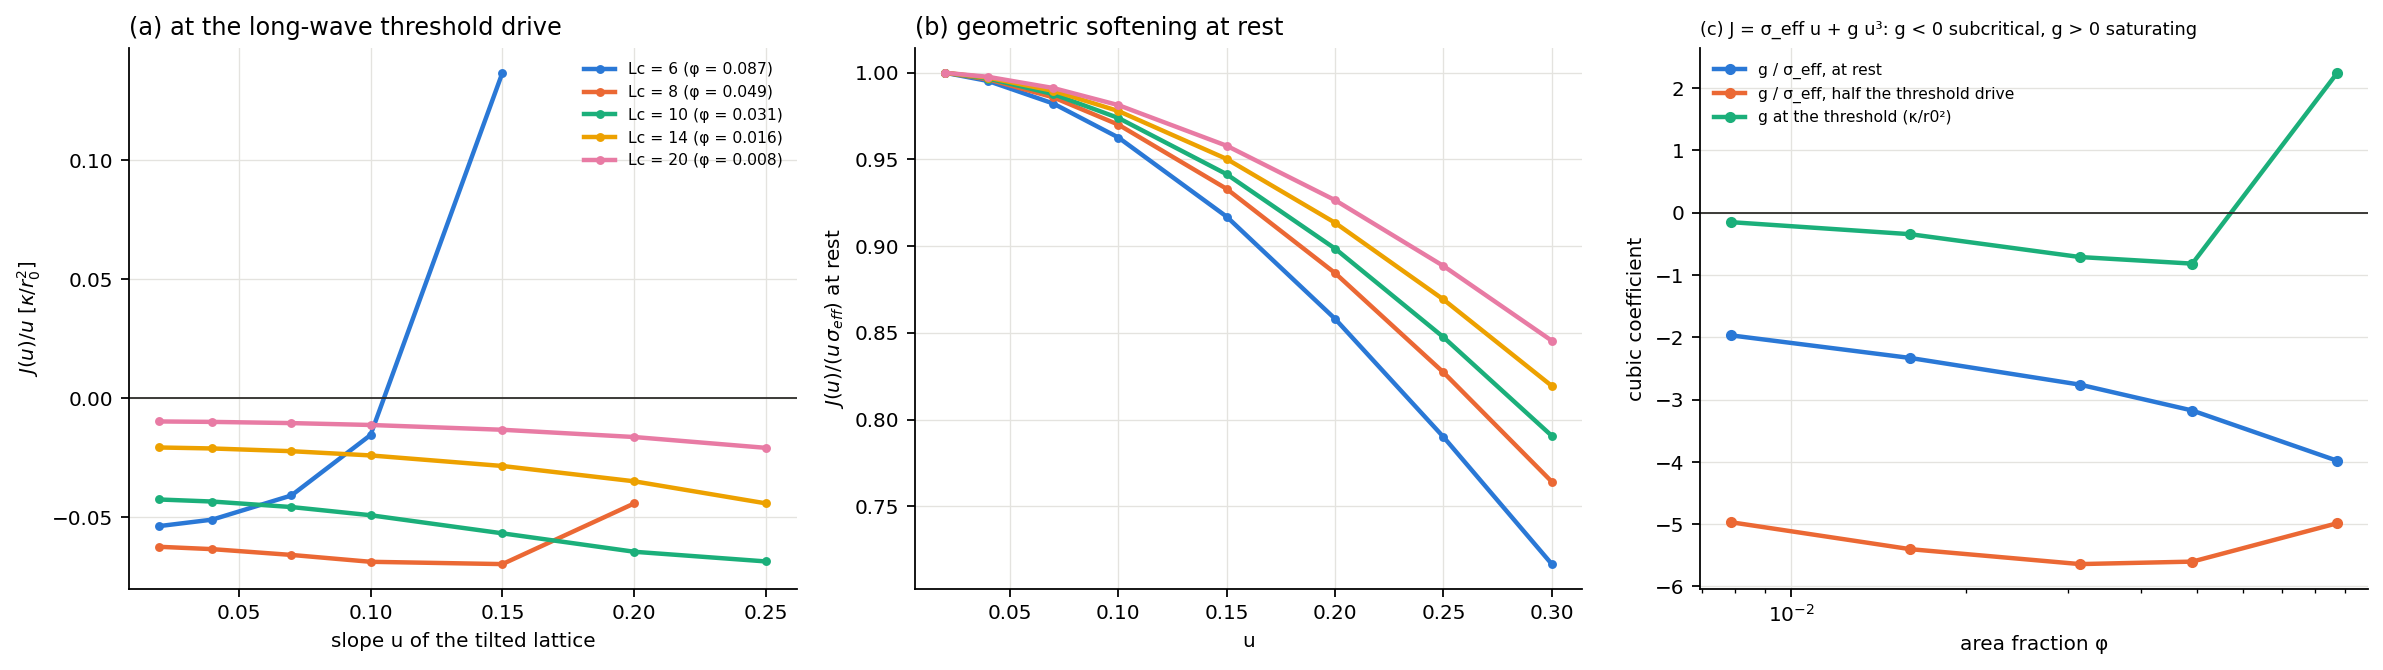
\includegraphics[width=\linewidth,height=86mm,keepaspectratio]{figures/membrane_r4_lattice_nonlinear.png}\captionof{figure}[Archived figure]{Nonlinear tilted-cell stress and geometric softening. Frozen flat-state flow is used; the small-slope cubic changes sign between intermediate and dense arrays, while the driven linear coefficient differs modestly from the dynamic Bloch value. \textit{Source:} \path{Ruben/membrane_stability/figures/r4_lattice_nonlinear.png}. First added 2026-10-01.}\end{center}
\clearpage
\begin{center}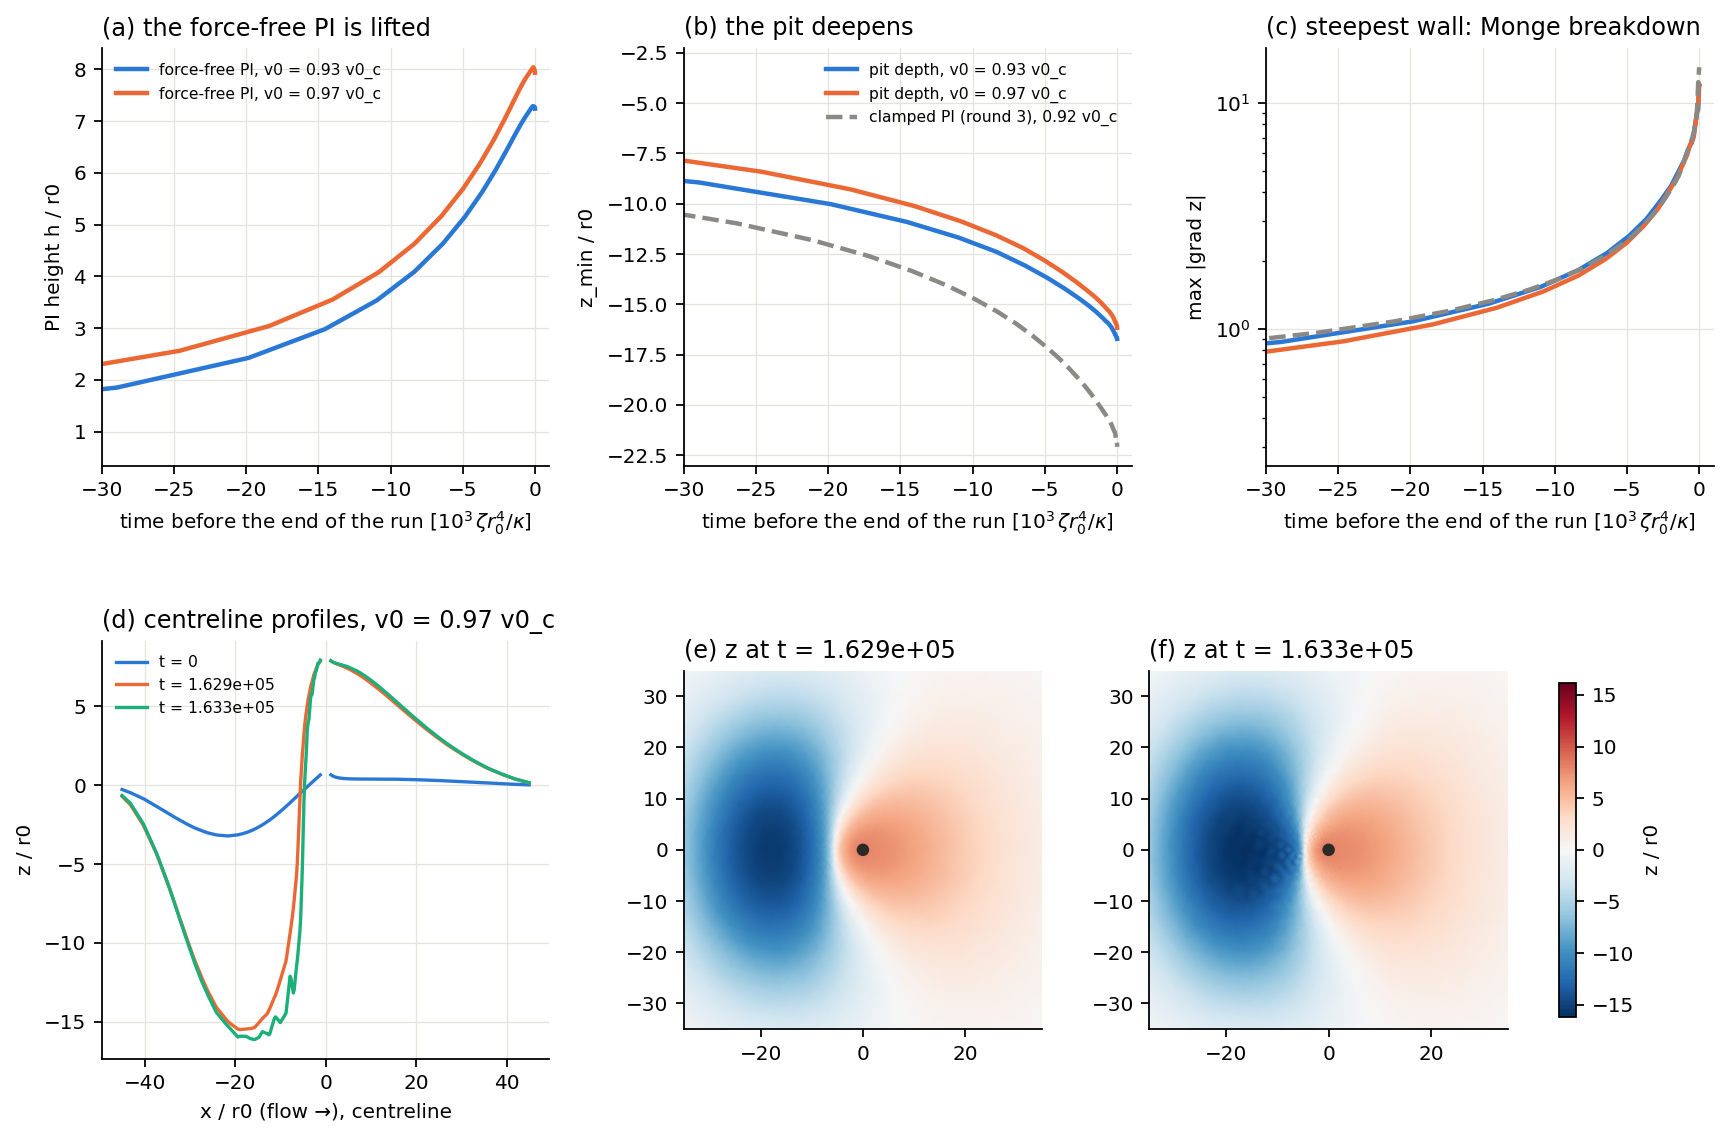
\includegraphics[width=\linewidth,height=182mm,keepaspectratio]{figures/membrane_r4_post_snap_forcefree.png}\captionof{figure}[Archived figure]{Force-free protein lift during upstream collapse. The protein rises onto a downstream crest and the wall steepens; cutoff-force consistency deteriorates at the last slopes. \textit{Source:} \path{Ruben/membrane_stability/figures/r4_post_snap_forcefree.png}. First added 2026-10-01.}\end{center}
\clearpage
\begin{center}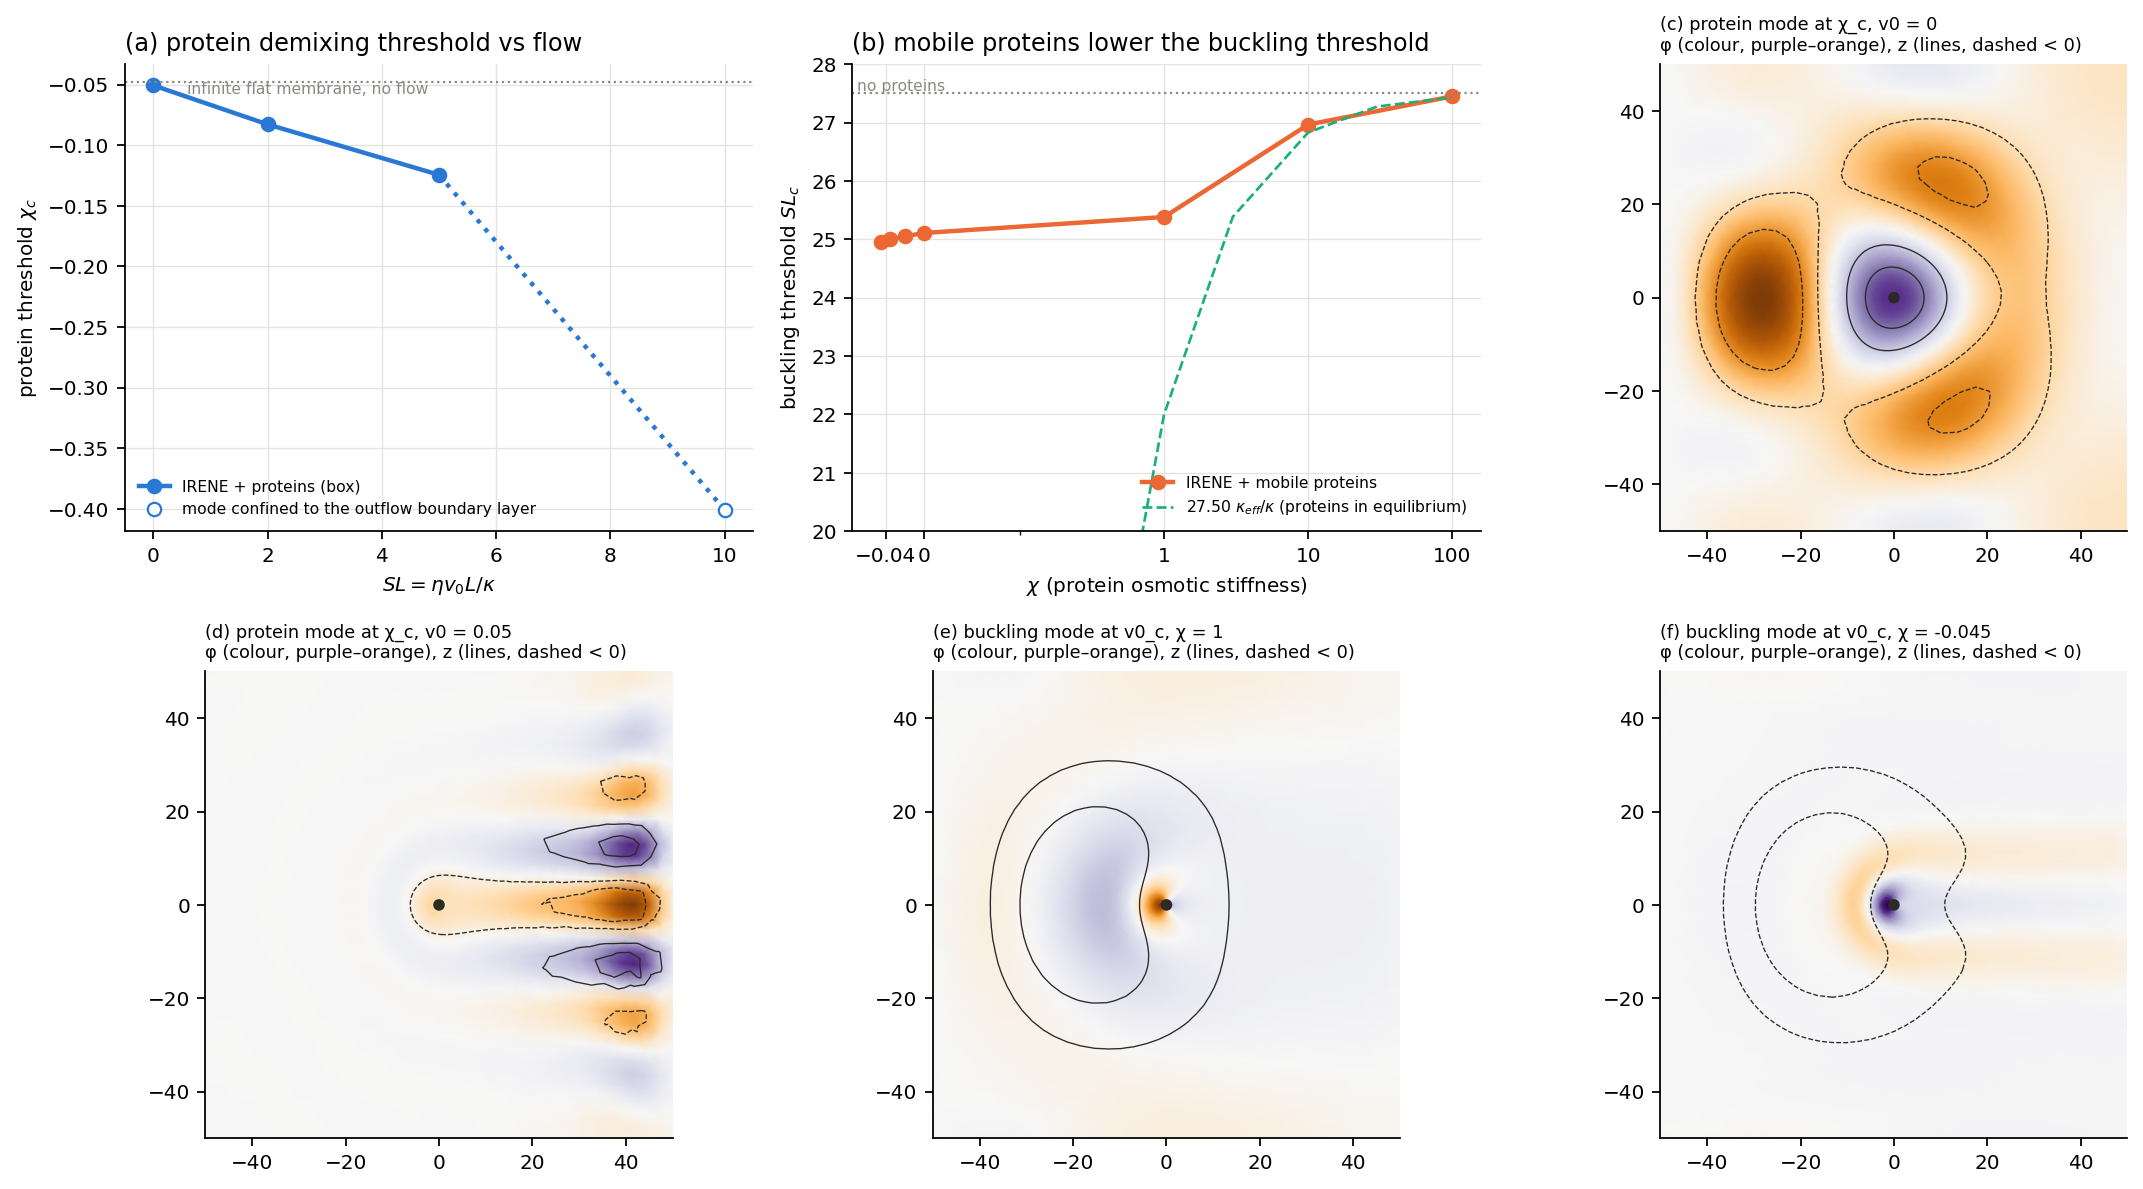
\includegraphics[width=\linewidth,height=182mm,keepaspectratio]{figures/membrane_r4_proteins.png}\captionof{figure}[Archived figure]{Earlier mobile-protein thresholds with no-flux outflow. The high-flow demixing mode is an outflow-layer artifact. The final absorbing-outflow mobility study replaces those high-flow thresholds. \textit{Source:} \path{Ruben/membrane_stability/figures/r4_proteins.png}. First added 2026-10-01.}\end{center}
\clearpage
\begin{center}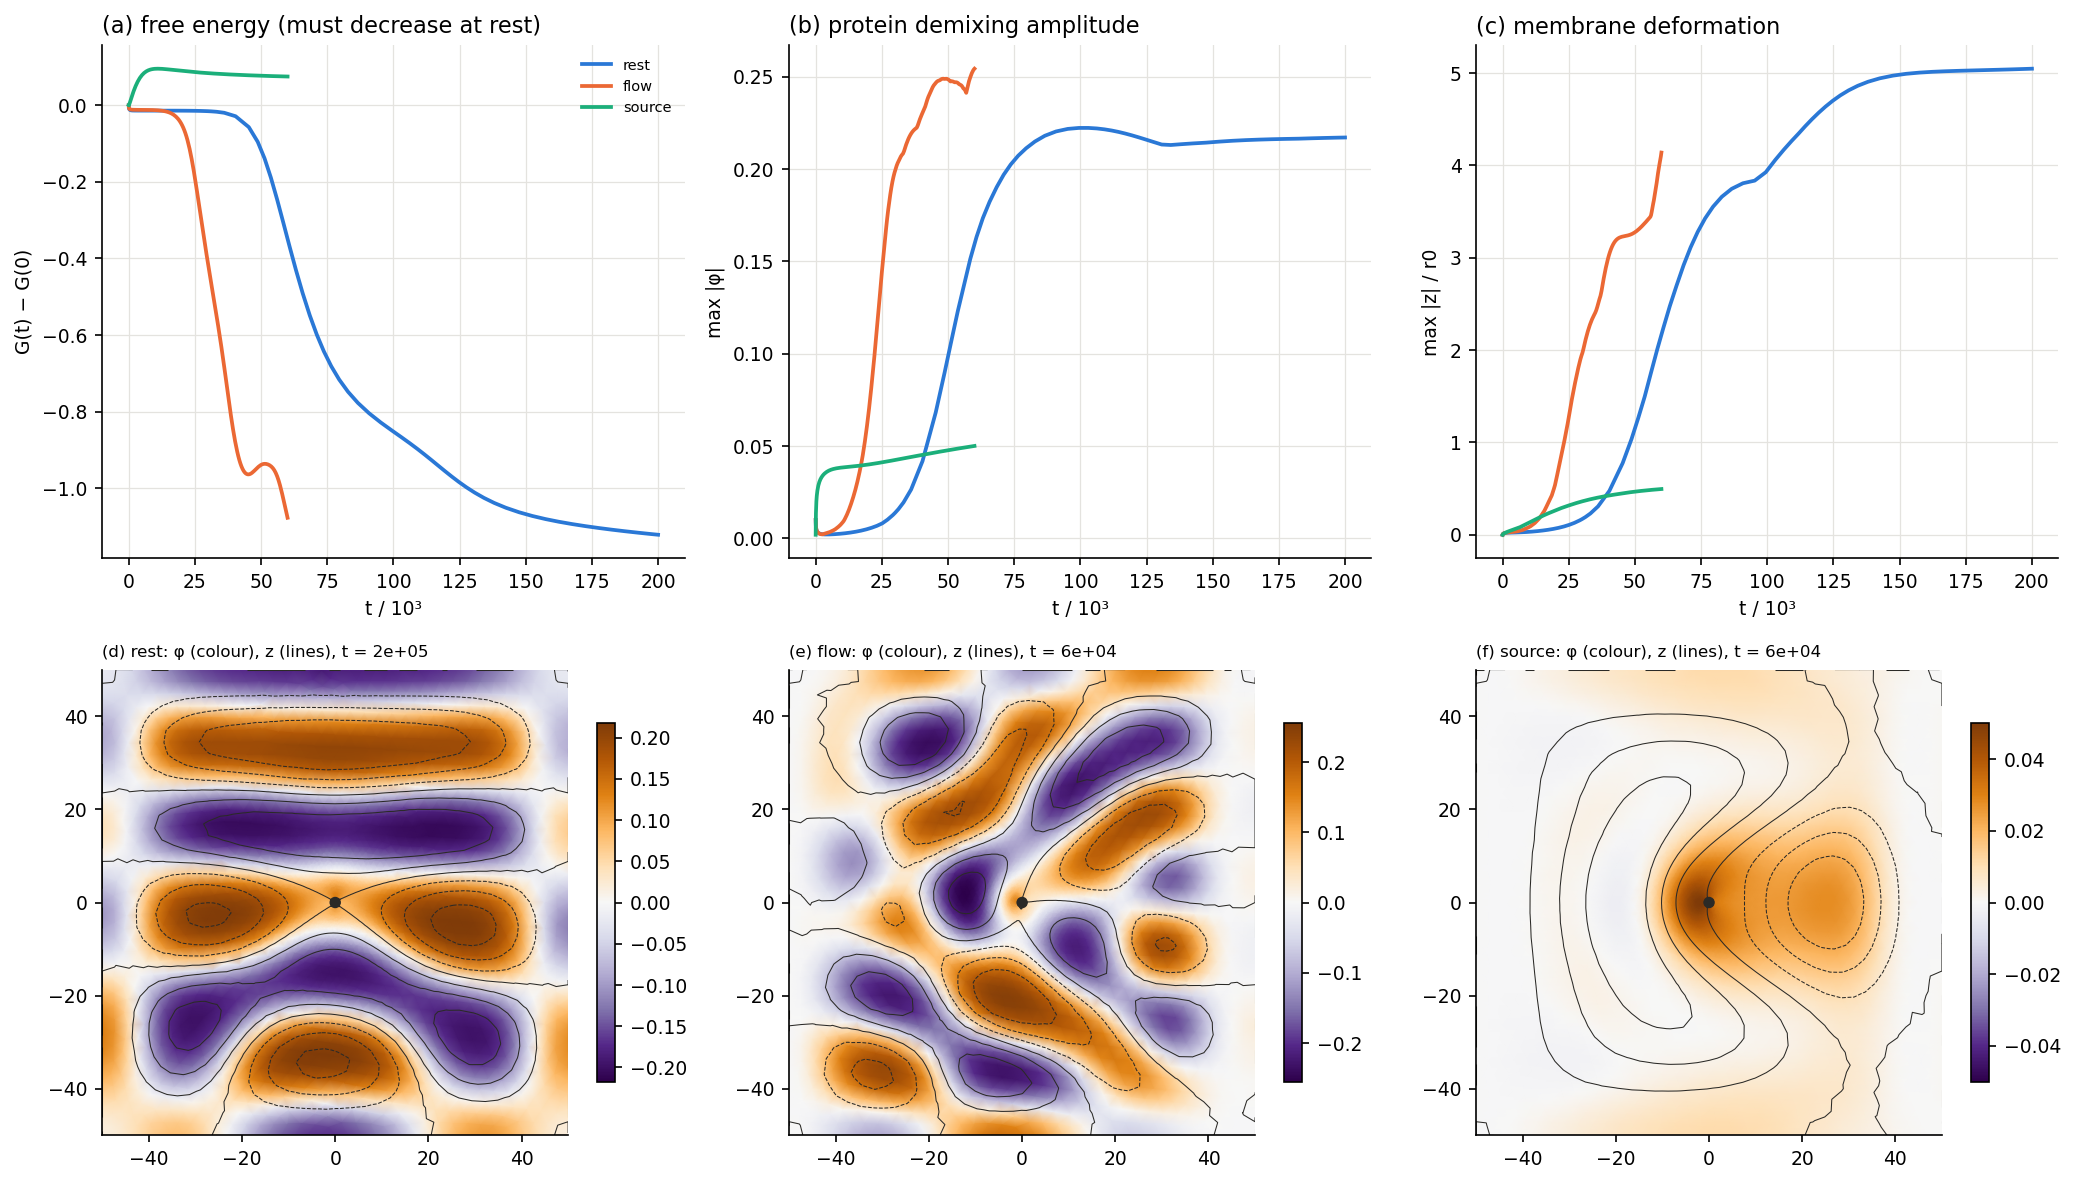
\includegraphics[width=\linewidth,height=182mm,keepaspectratio]{figures/membrane_r5_proteins_dyn.png}\captionof{figure}[Archived figure]{Consistent nonlinear mobile-protein dynamics: no-flow energy relaxation, amplitude saturation, flow-elongated domains, and a source-driven plume. Open reservoirs/sinks mean global protein conservation must include boundary exchange. \textit{Source:} \path{Ruben/membrane_stability/figures/r5_proteins_dyn.png}. First added 2026-10-02.}\end{center}
\clearpage
\begin{center}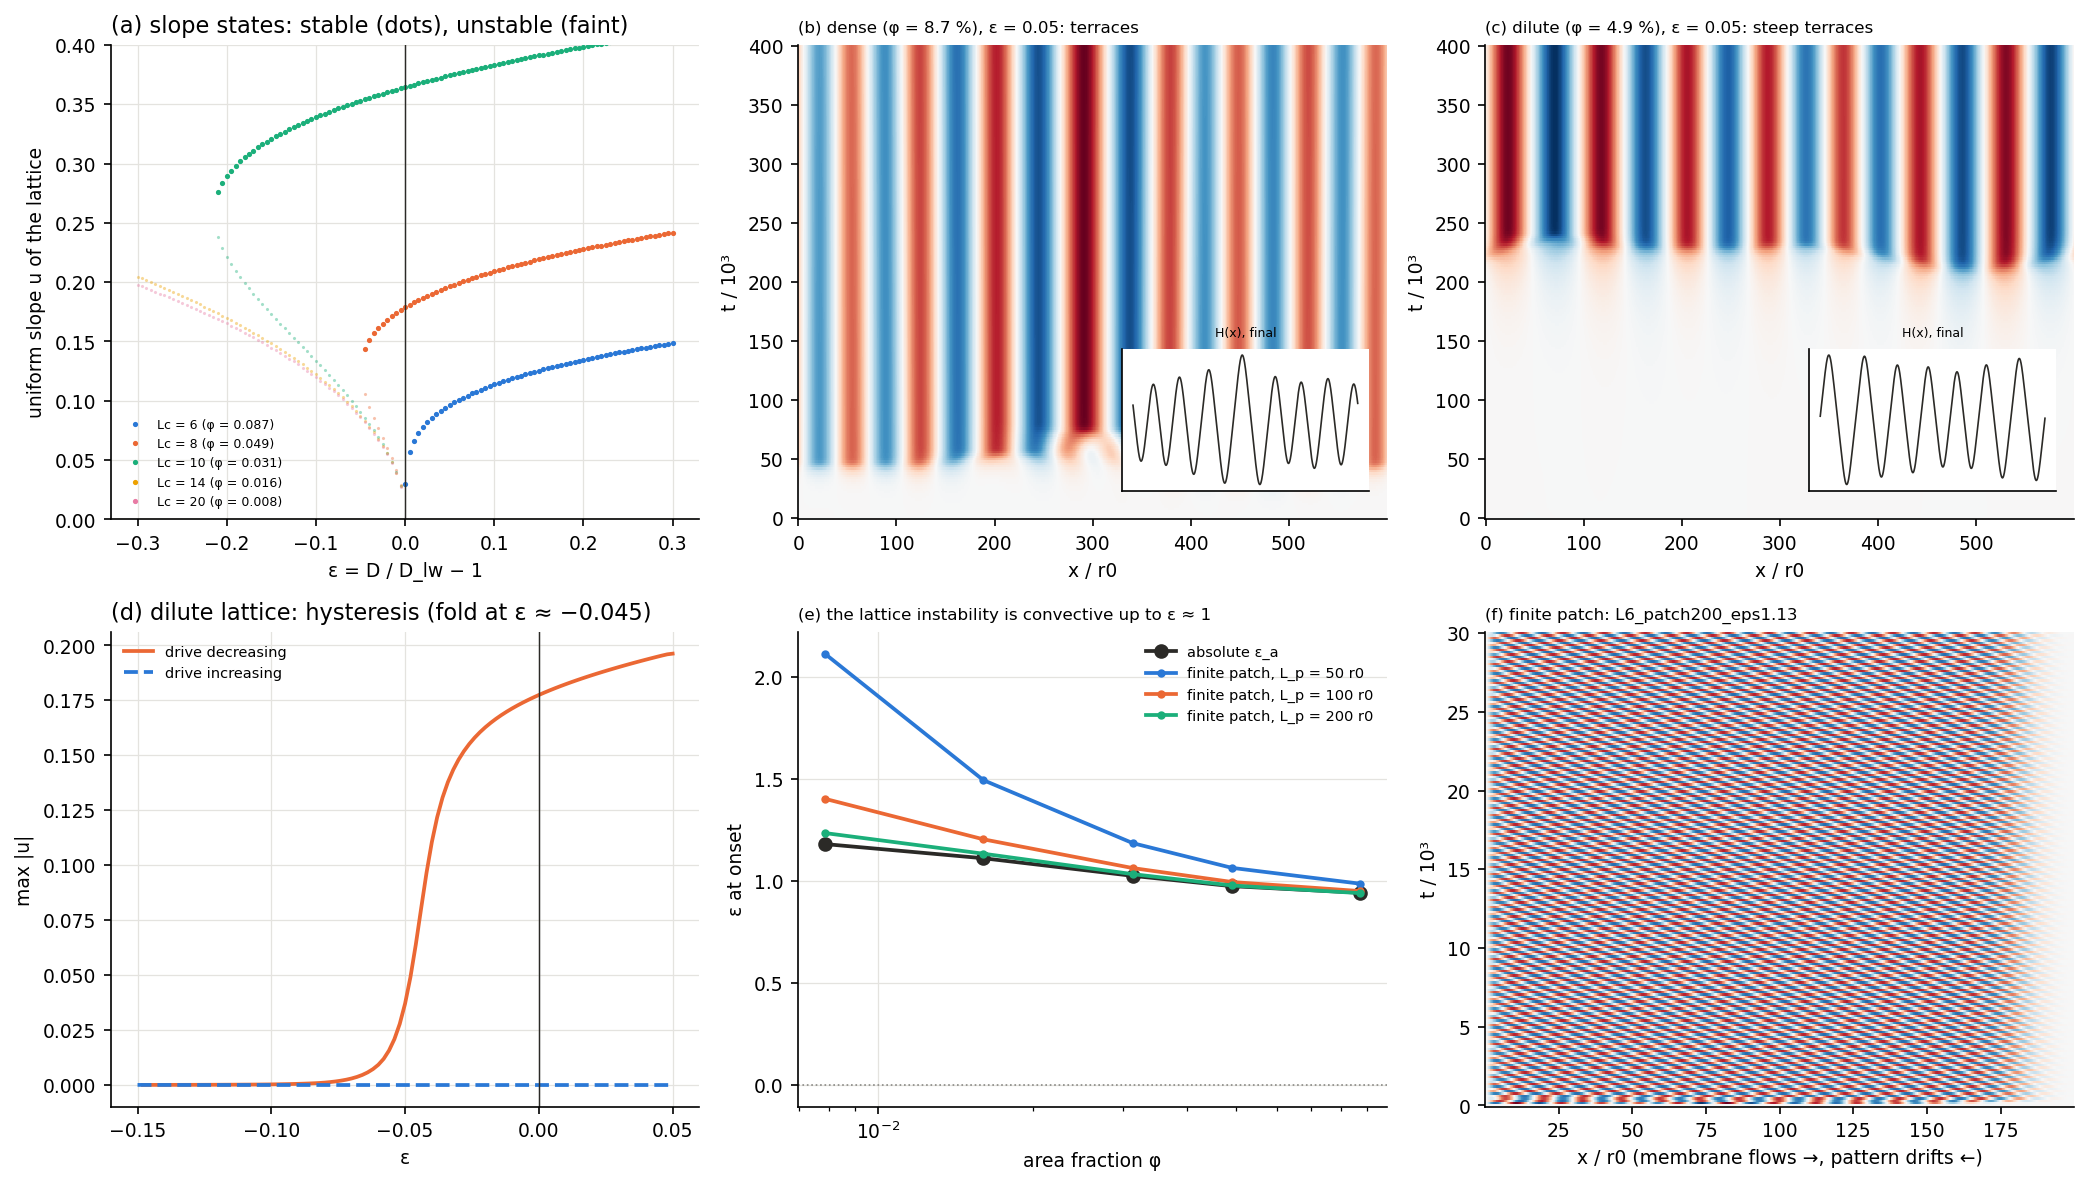
\includegraphics[width=\linewidth,height=182mm,keepaspectratio]{figures/membrane_r5_slope_equation.png}\captionof{figure}[Archived figure]{One-dimensional homogenized lattice dynamics: continuous or hysteretic slope states, coarsening terraces, and finite-patch drift. The absolute-threshold estimate uses a long-wave model near the edge of its spatial validity. \textit{Source:} \path{Ruben/membrane_stability/figures/r5_slope_equation.png}. First added 2026-10-02.}\end{center}
\clearpage
\begin{center}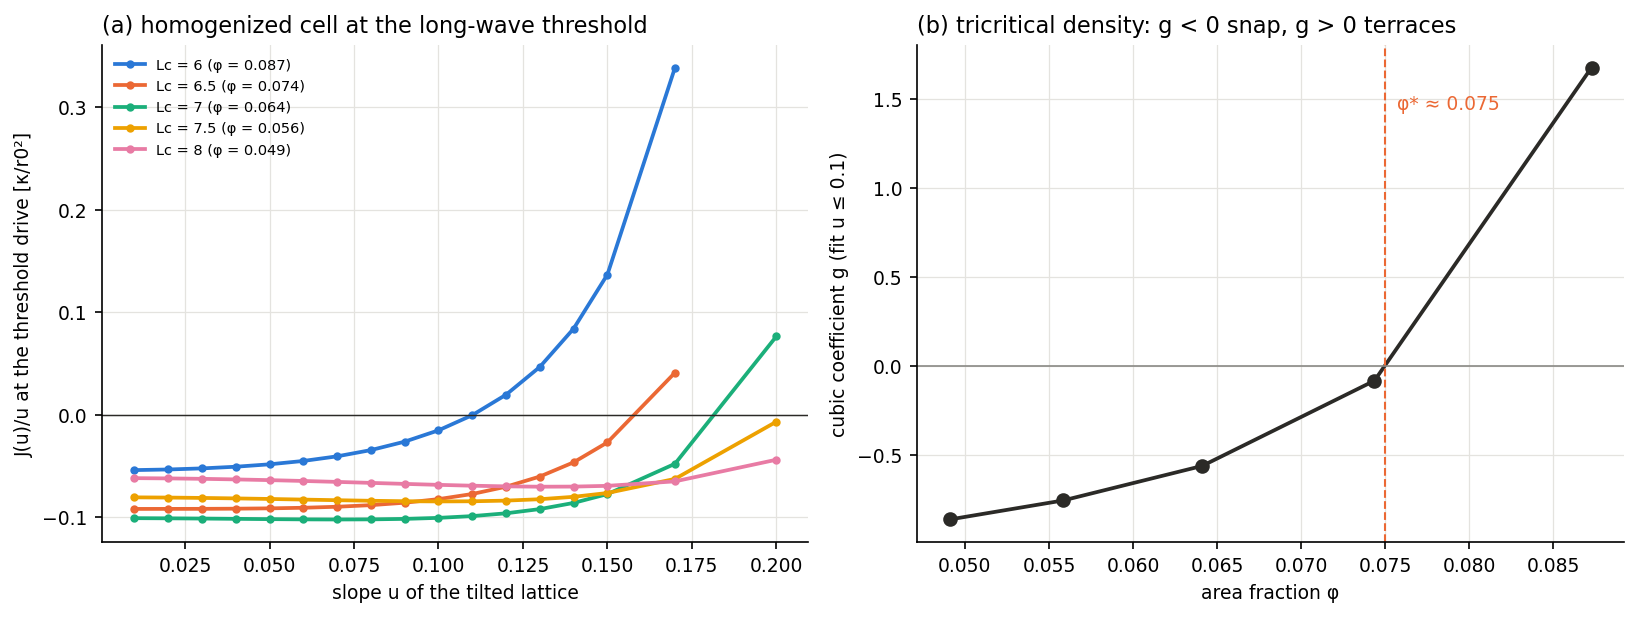
\includegraphics[width=\linewidth,height=86mm,keepaspectratio]{figures/membrane_r5_tricritical.png}\captionof{figure}[Archived figure]{Small-slope nonlinear-cell fits locating the cubic sign change near anchored-disc area fraction 7.5 percent. This onset diagnostic uses a narrower fitting window than the later two-dimensional finite-amplitude polynomial. \textit{Source:} \path{Ruben/membrane_stability/figures/r5_tricritical.png}. First added 2026-10-02.}\end{center}
\begin{center}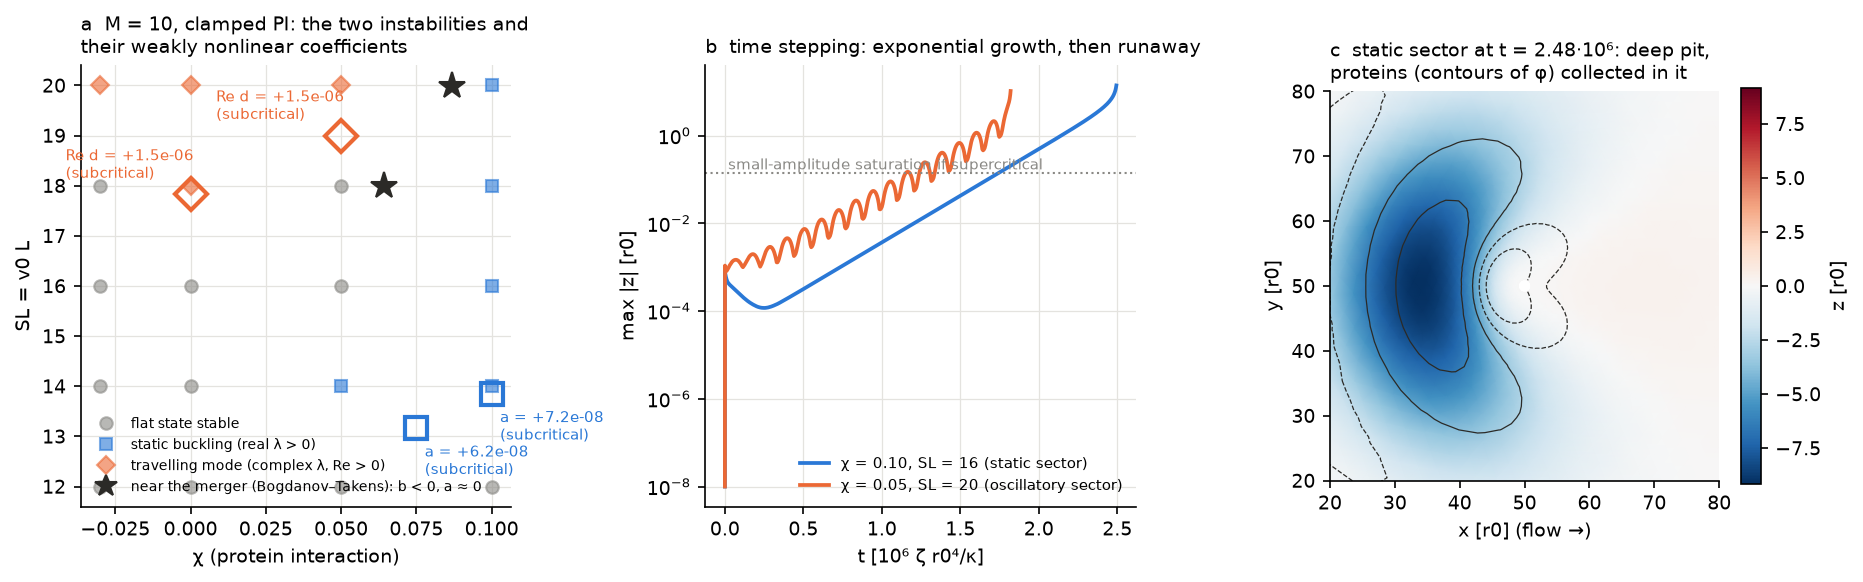
\includegraphics[width=\linewidth,height=86mm,keepaspectratio]{figures/membrane_r6_codim2.png}\captionof{figure}[Archived figure]{Clamped-protein, intermediate-mobility eigenvalue sectors and nonlinear runaway. The nearly vanishing eigenvalues motivate a degenerate Bogdanov-Takens-type interpretation; an exact double-zero location and quintic unfolding remain unresolved. \textit{Source:} \path{Ruben/membrane_stability/figures/r6_codim2.png}. First added 2026-10-03.}\end{center}
\clearpage
\begin{center}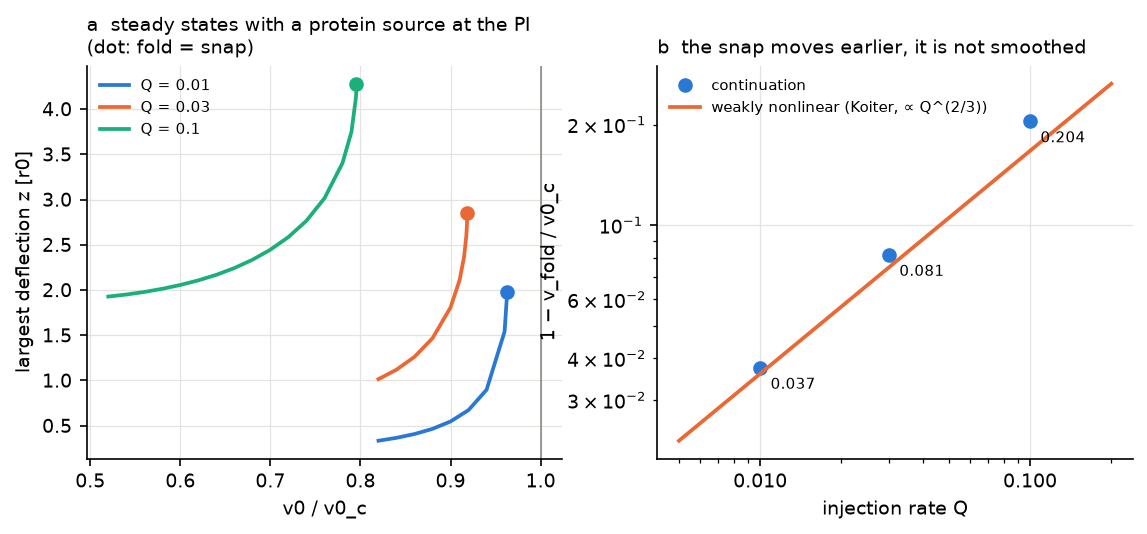
\includegraphics[width=\linewidth,height=86mm,keepaspectratio]{figures/membrane_r6_wake.png}\captionof{figure}[Archived figure]{Source-induced folds and the Koiter prediction. Recruitment is an imperfection that advances rather than removes the snap. The largest-source case is outside the smallest-amplitude cubic regime. \textit{Source:} \path{Ruben/membrane_stability/figures/r6_wake.png}. First added 2026-10-03.}\end{center}
\begin{center}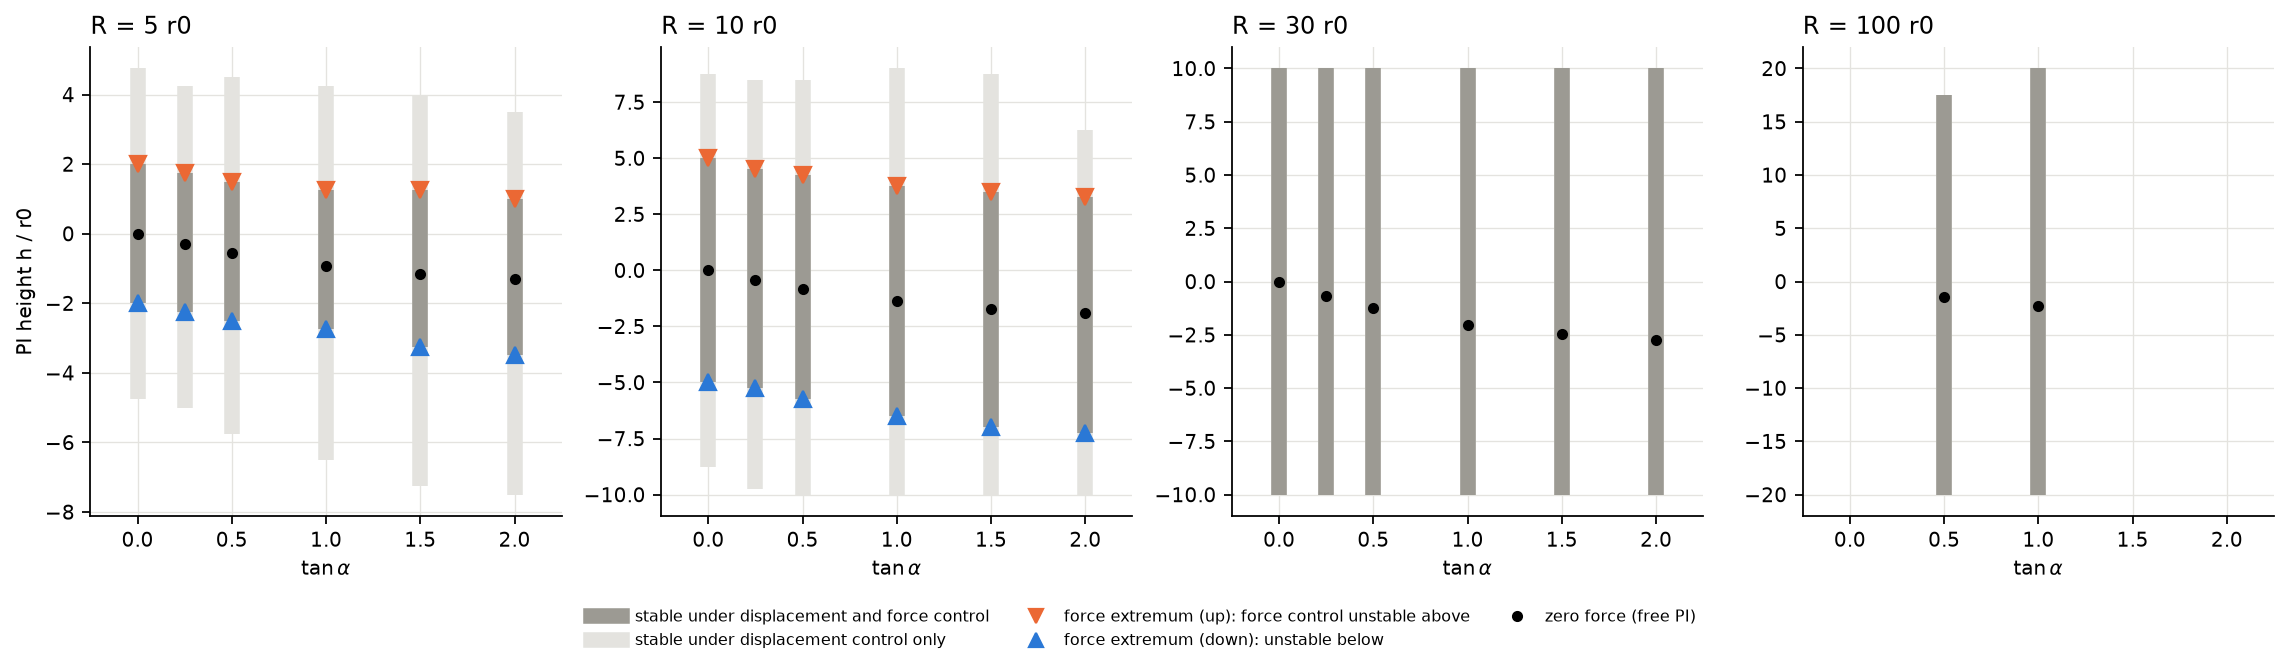
\includegraphics[width=\linewidth,height=86mm,keepaspectratio]{figures/membrane_ring_stability_diagram.png}\captionof{figure}[Archived figure]{Height/contact-slope ring stability diagram over the computed windows. The force-control boundaries are virtual-work force extrema; height-controlled branches remain stable. Grey endpoints indicate limits of the sampled branch. \textit{Source:} \path{Ruben/membrane_stability/figures/ring_stability_diagram.png}. First added 2026-09-30.}\end{center}
\clearpage
\begin{center}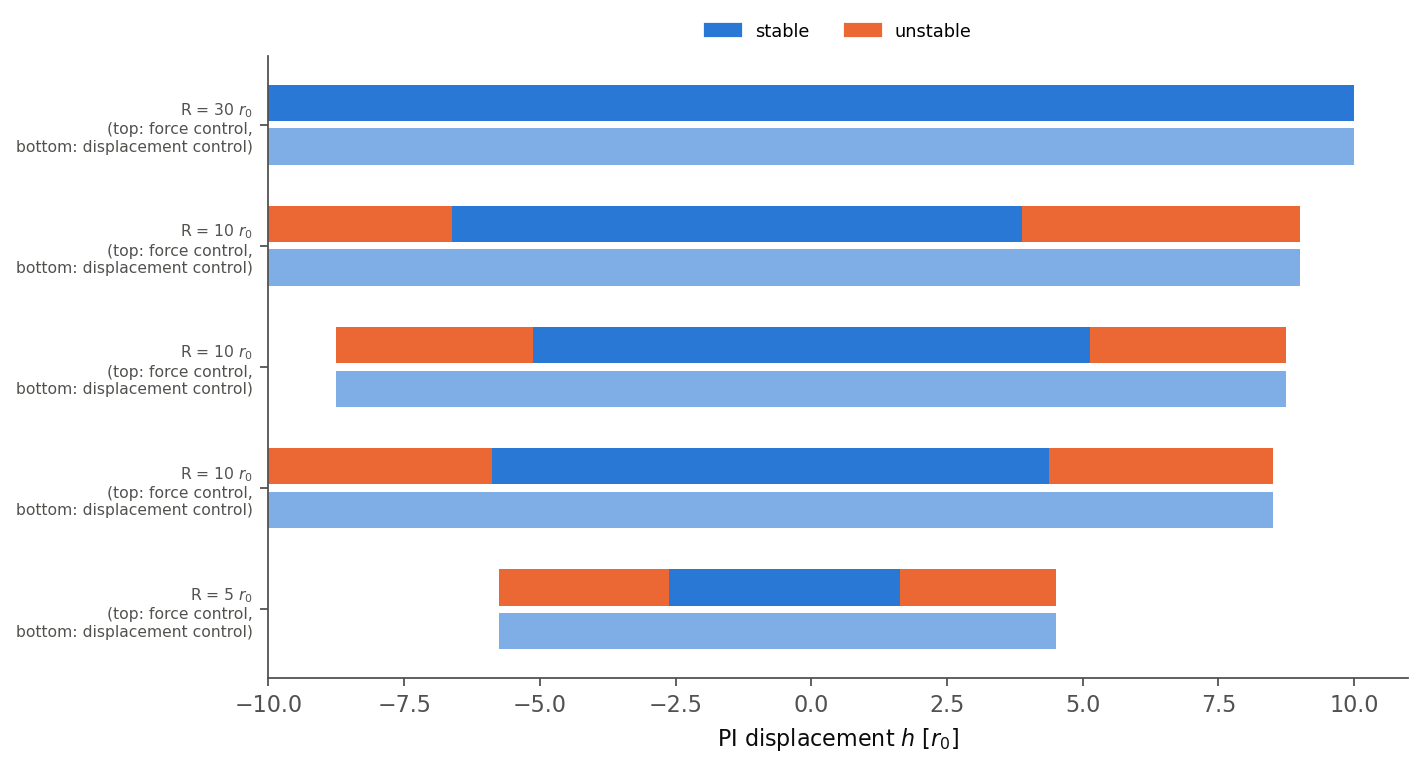
\includegraphics[width=\linewidth,height=182mm,keepaspectratio]{figures/membrane_stability_summary.png}\captionof{figure}[Archived figure]{Ring control-ensemble summary. Force-controlled softening segments are unstable even when the fixed-height shape spectrum remains stable. \textit{Source:} \path{Ruben/membrane_stability/figures/stability_summary.png}. First added 2026-09-29.}\end{center}
\clearpage
\begin{center}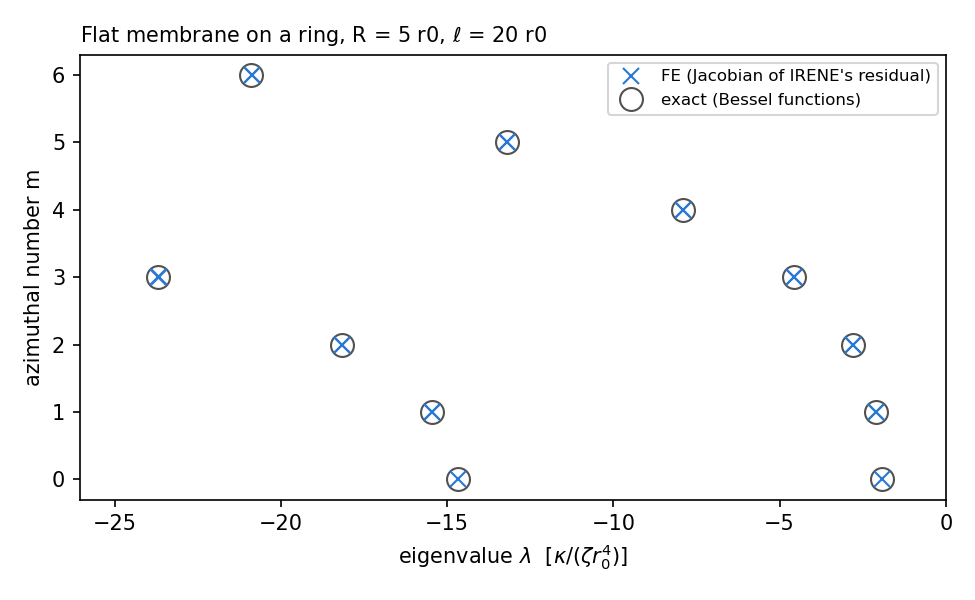
\includegraphics[width=\linewidth,height=182mm,keepaspectratio]{figures/membrane_flat_ring_R5_coarse.png}\captionof{figure}[Archived figure]{Coarse-mesh flat-annulus eigenvalues by azimuthal number compared with the exact Bessel spectrum. This is a separate asset from the fine-mesh check with the same original basename. \textit{Source:} \path{Ruben/membrane_stability/results/checks/flat_ring_R5/check_flat_membrane.png}. First added 2026-09-29.}\end{center}
\clearpage
\begin{center}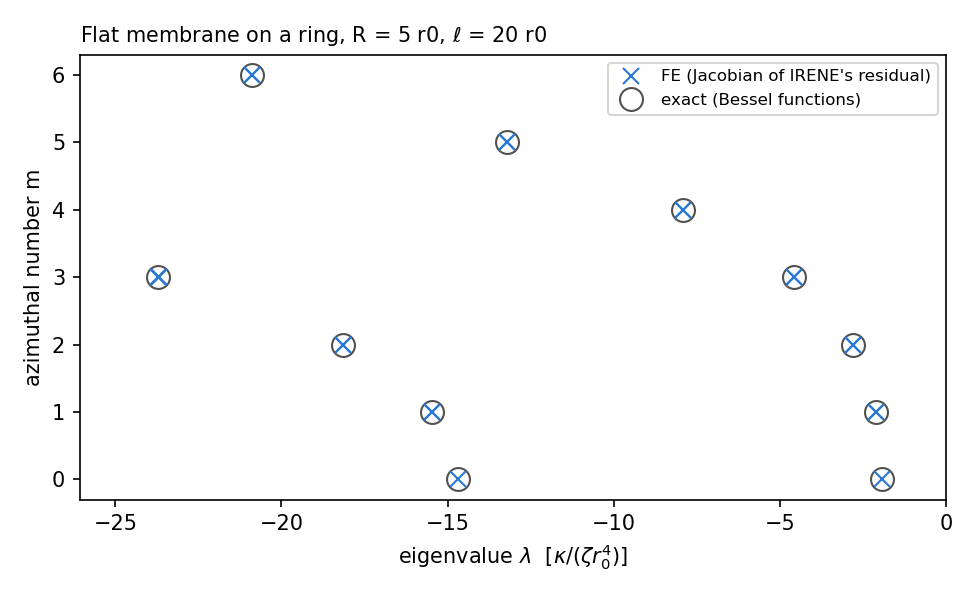
\includegraphics[width=\linewidth,height=182mm,keepaspectratio]{figures/membrane_flat_ring_R5_fine.png}\captionof{figure}[Archived figure]{Fine-mesh flat-annulus spectrum. Refinement reduces the maximum discrepancy to about 2.3 times ten to the minus four across the tested twenty eigenvalues. \textit{Source:} \path{Ruben/membrane_stability/results/checks/flat_ring_R5_fine/check_flat_membrane.png}. First added 2026-09-29.}\end{center}
\clearpage

\clearpage
\section{Animation storyboards and bundled media}
\begin{center}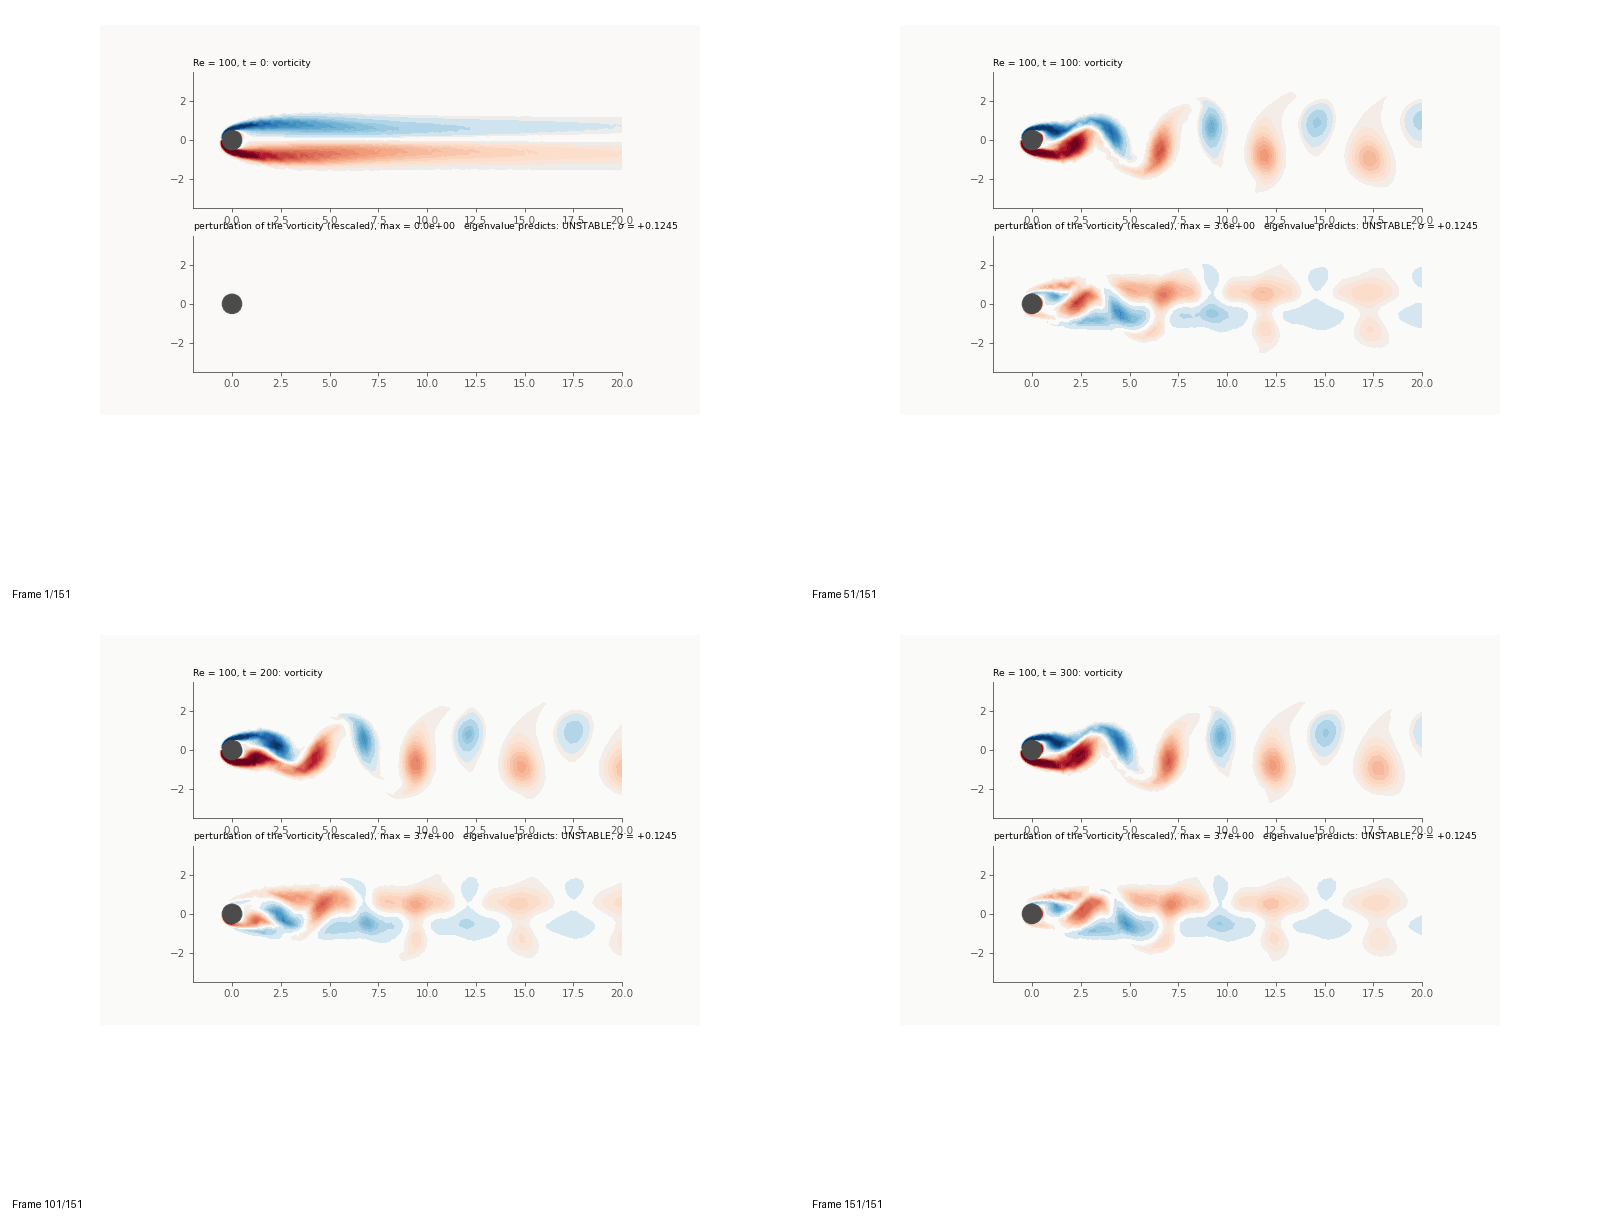
\includegraphics[width=\linewidth,height=170mm,keepaspectratio]{animation_stills/wake_dns_Re100_vorticity.png}\captionof{figure}[Archived figure]{Cylinder benchmark at Reynolds number one hundred: nonlinear saturated vortex shedding. Four ordered frames are selected by frame index; spacing is not asserted to be uniform in physical time. \textit{Original GIF:} \path{research/Navier_Stokes_Inflow/stability/figures/dns_Re100_vorticity.gif}. First added 2026-09-29.}\end{center}
\noindent\textit{Playback file in this source package:} \path{figures/wake_dns_Re100_vorticity.gif}.\clearpage
\begin{center}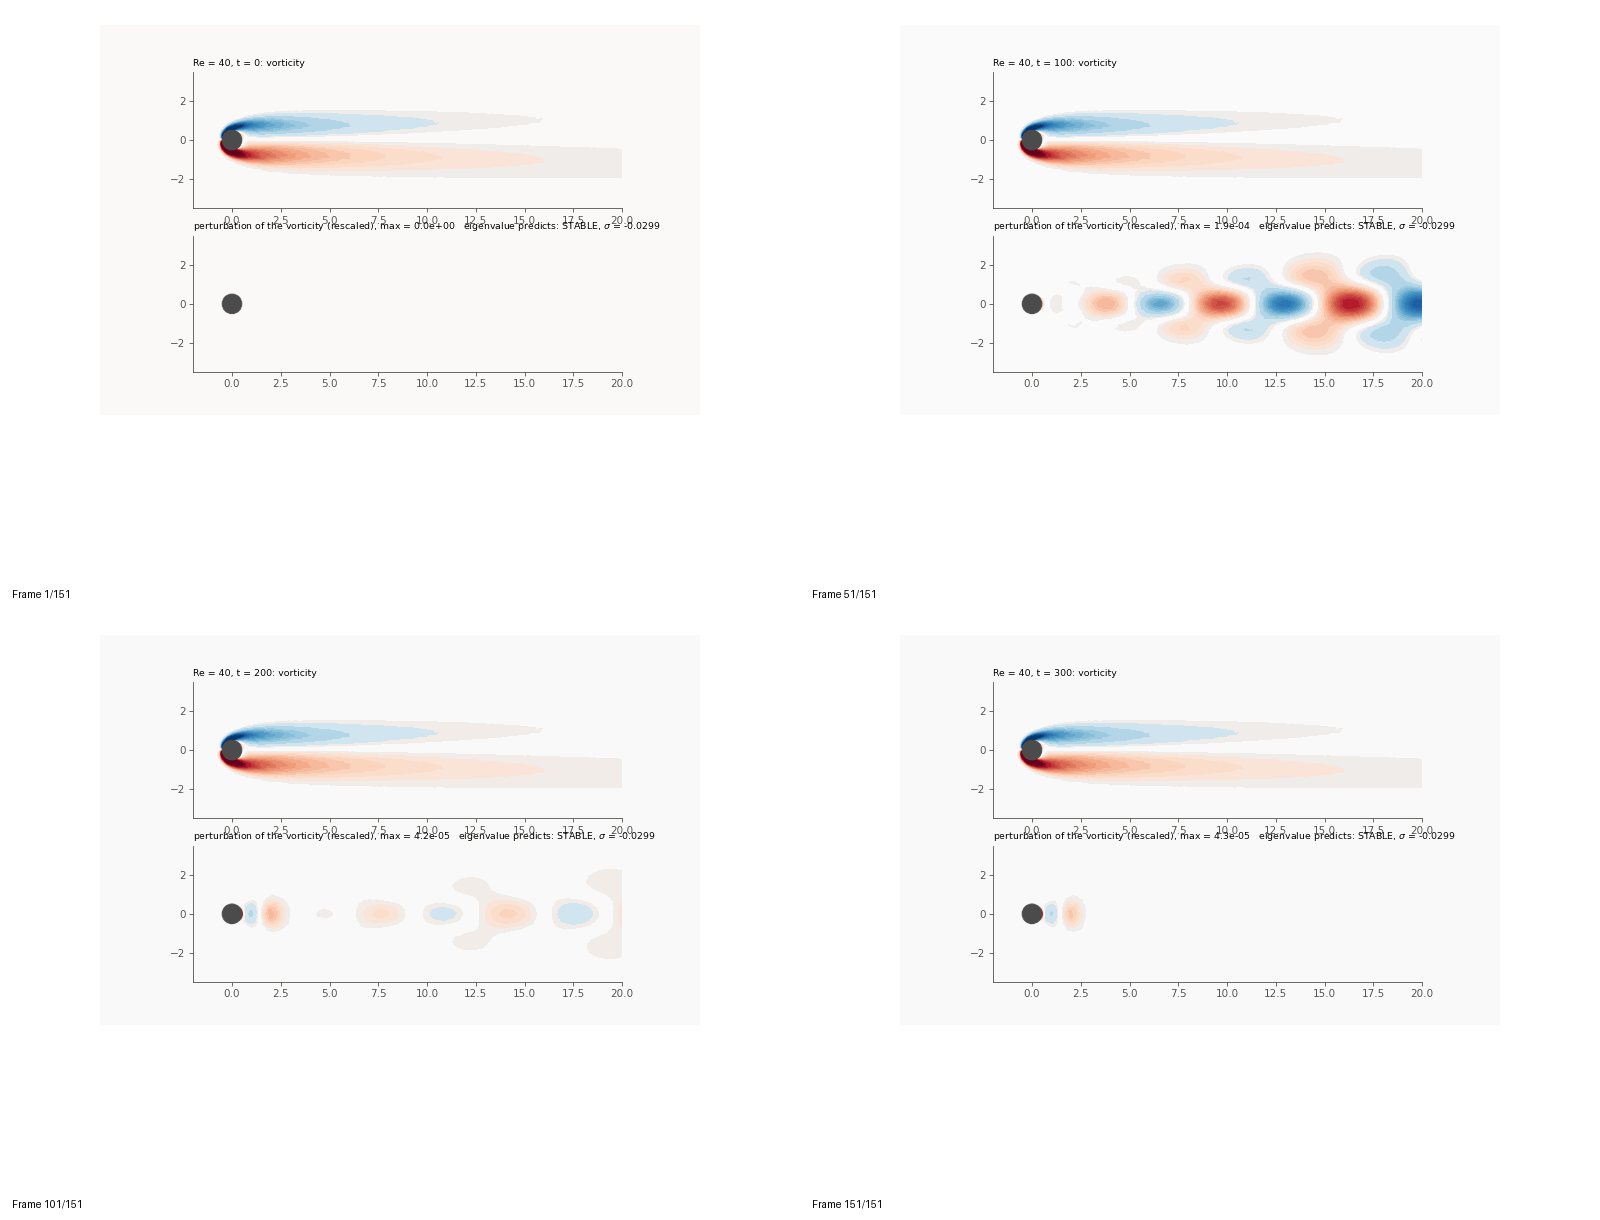
\includegraphics[width=\linewidth,height=170mm,keepaspectratio]{animation_stills/wake_dns_Re40_vorticity.png}\captionof{figure}[Archived figure]{Cylinder benchmark below onset: an initial perturbation decays to a steady symmetric wake. Four ordered frames are selected by frame index; spacing is not asserted to be uniform in physical time. \textit{Original GIF:} \path{research/Navier_Stokes_Inflow/stability/figures/dns_Re40_vorticity.gif}. First added 2026-09-29.}\end{center}
\noindent\textit{Playback file in this source package:} \path{figures/wake_dns_Re40_vorticity.gif}.\clearpage
\begin{center}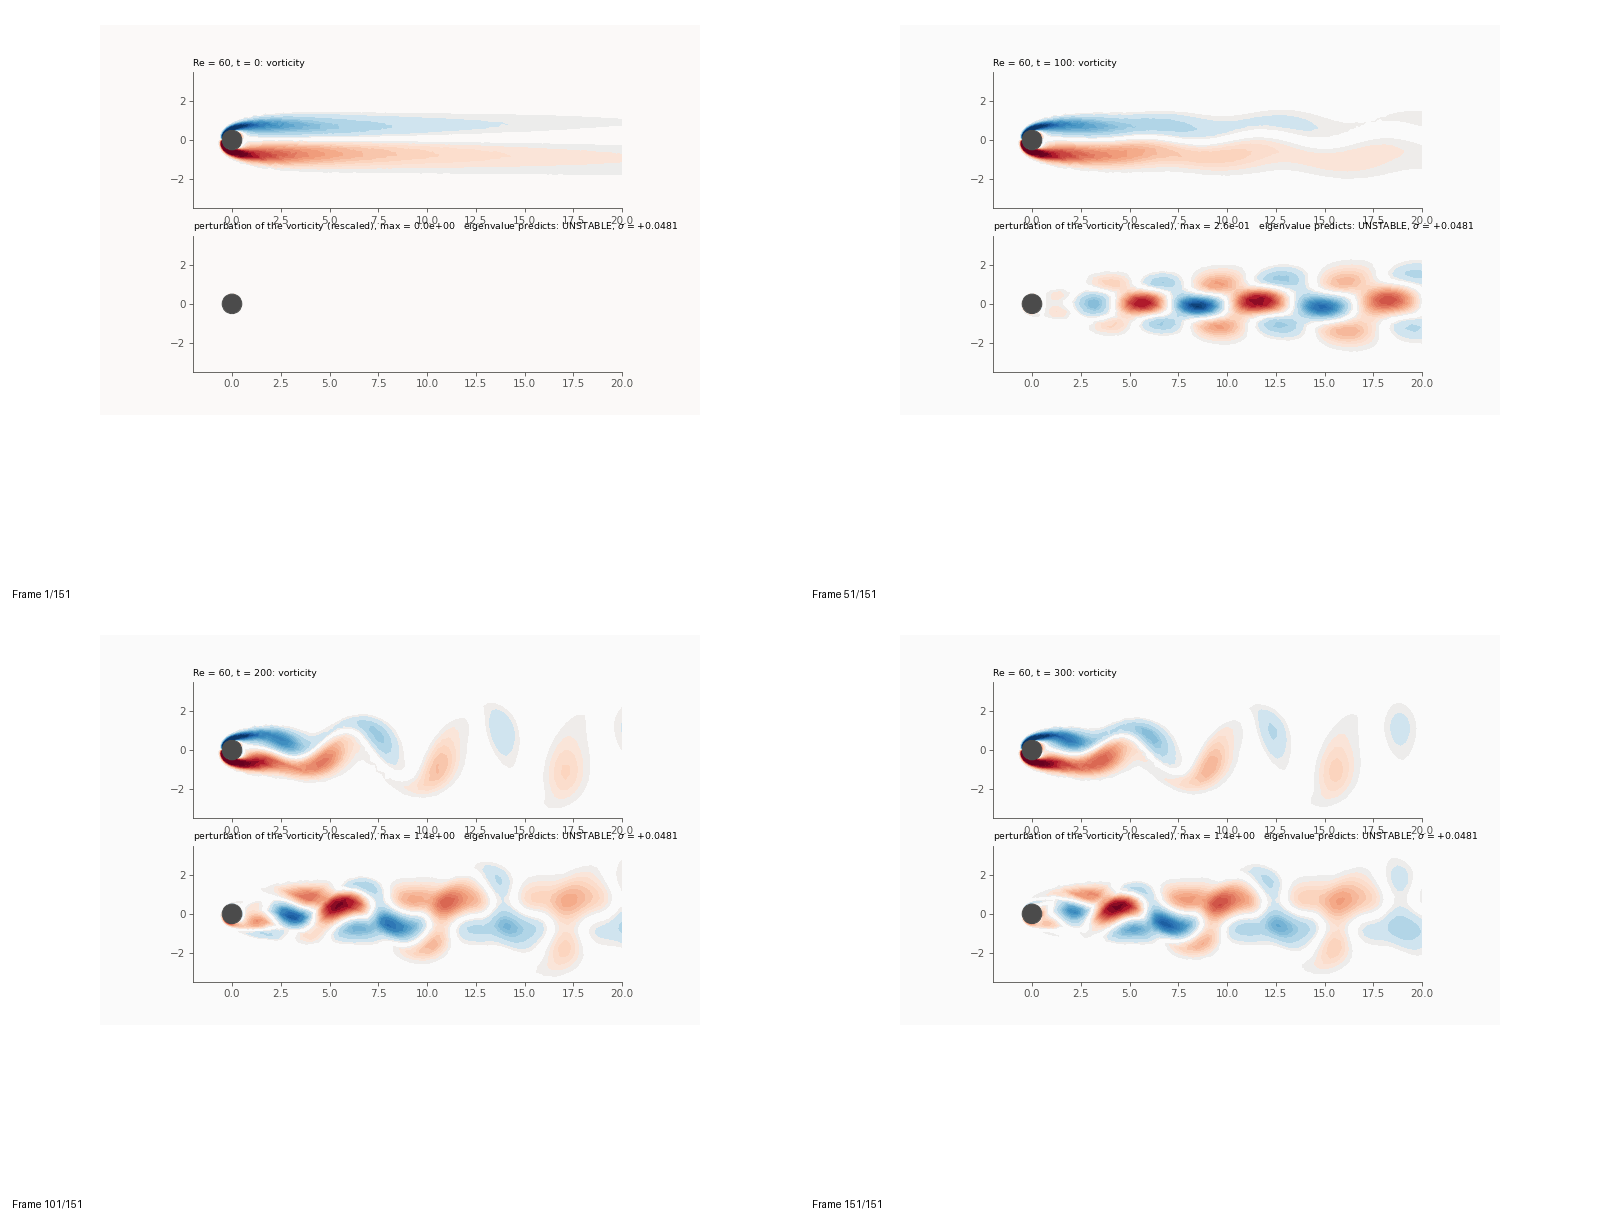
\includegraphics[width=\linewidth,height=170mm,keepaspectratio]{animation_stills/wake_dns_Re60_vorticity.png}\captionof{figure}[Archived figure]{Cylinder benchmark above onset: growing perturbations develop into a vortex street. Four ordered frames are selected by frame index; spacing is not asserted to be uniform in physical time. \textit{Original GIF:} \path{research/Navier_Stokes_Inflow/stability/figures/dns_Re60_vorticity.gif}. First added 2026-09-29.}\end{center}
\noindent\textit{Playback file in this source package:} \path{figures/wake_dns_Re60_vorticity.gif}.\clearpage
\begin{center}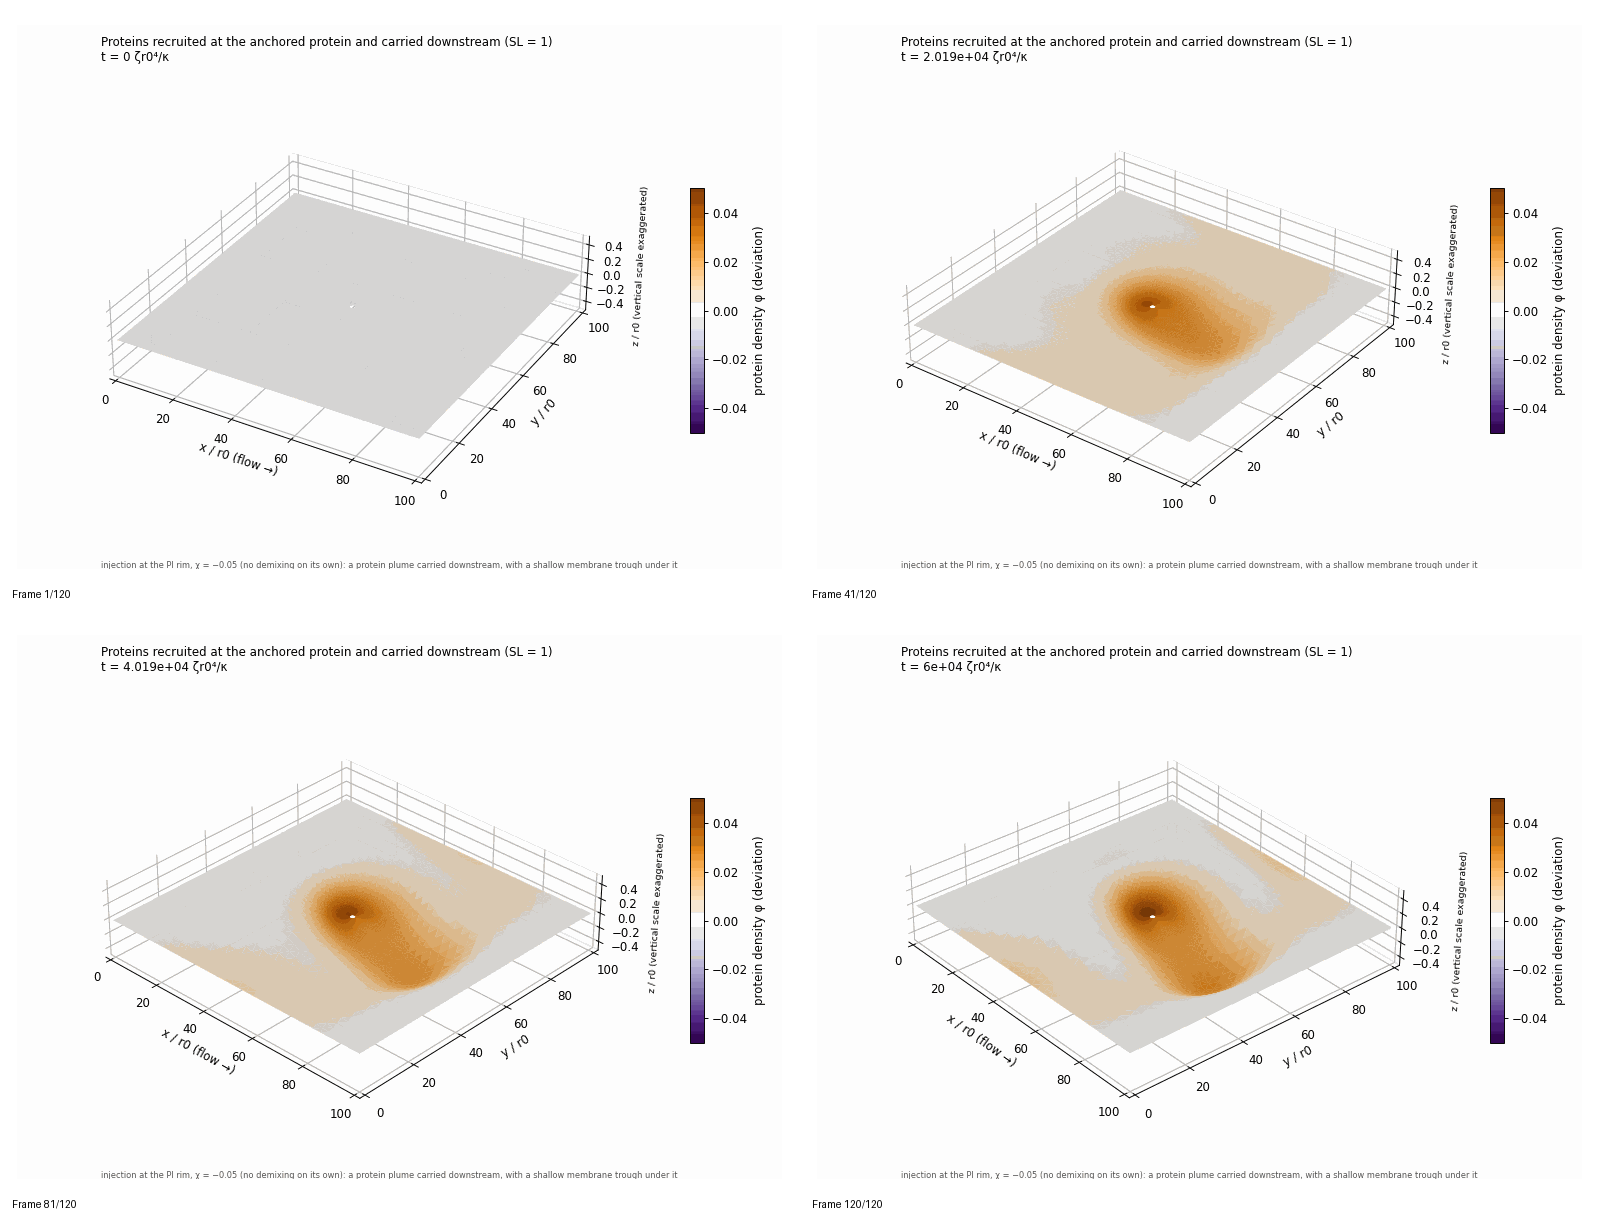
\includegraphics[width=\linewidth,height=170mm,keepaspectratio]{animation_stills/membrane_gif10_proteins_source_3d.png}\captionof{figure}[Archived figure]{Rim-source protein plume carried downstream with a shallow associated trough. The final run uses absorbing outflow. Four ordered frames are selected by frame index; spacing is not asserted to be uniform in physical time. \textit{Original GIF:} \path{research/membrane_stability/figures/gifs/gif10_proteins_source_3d.gif}. First added 2026-10-02.}\end{center}
\noindent\textit{Playback file in this source package:} \path{figures/membrane_gif10_proteins_source_3d.gif}.\clearpage
\begin{center}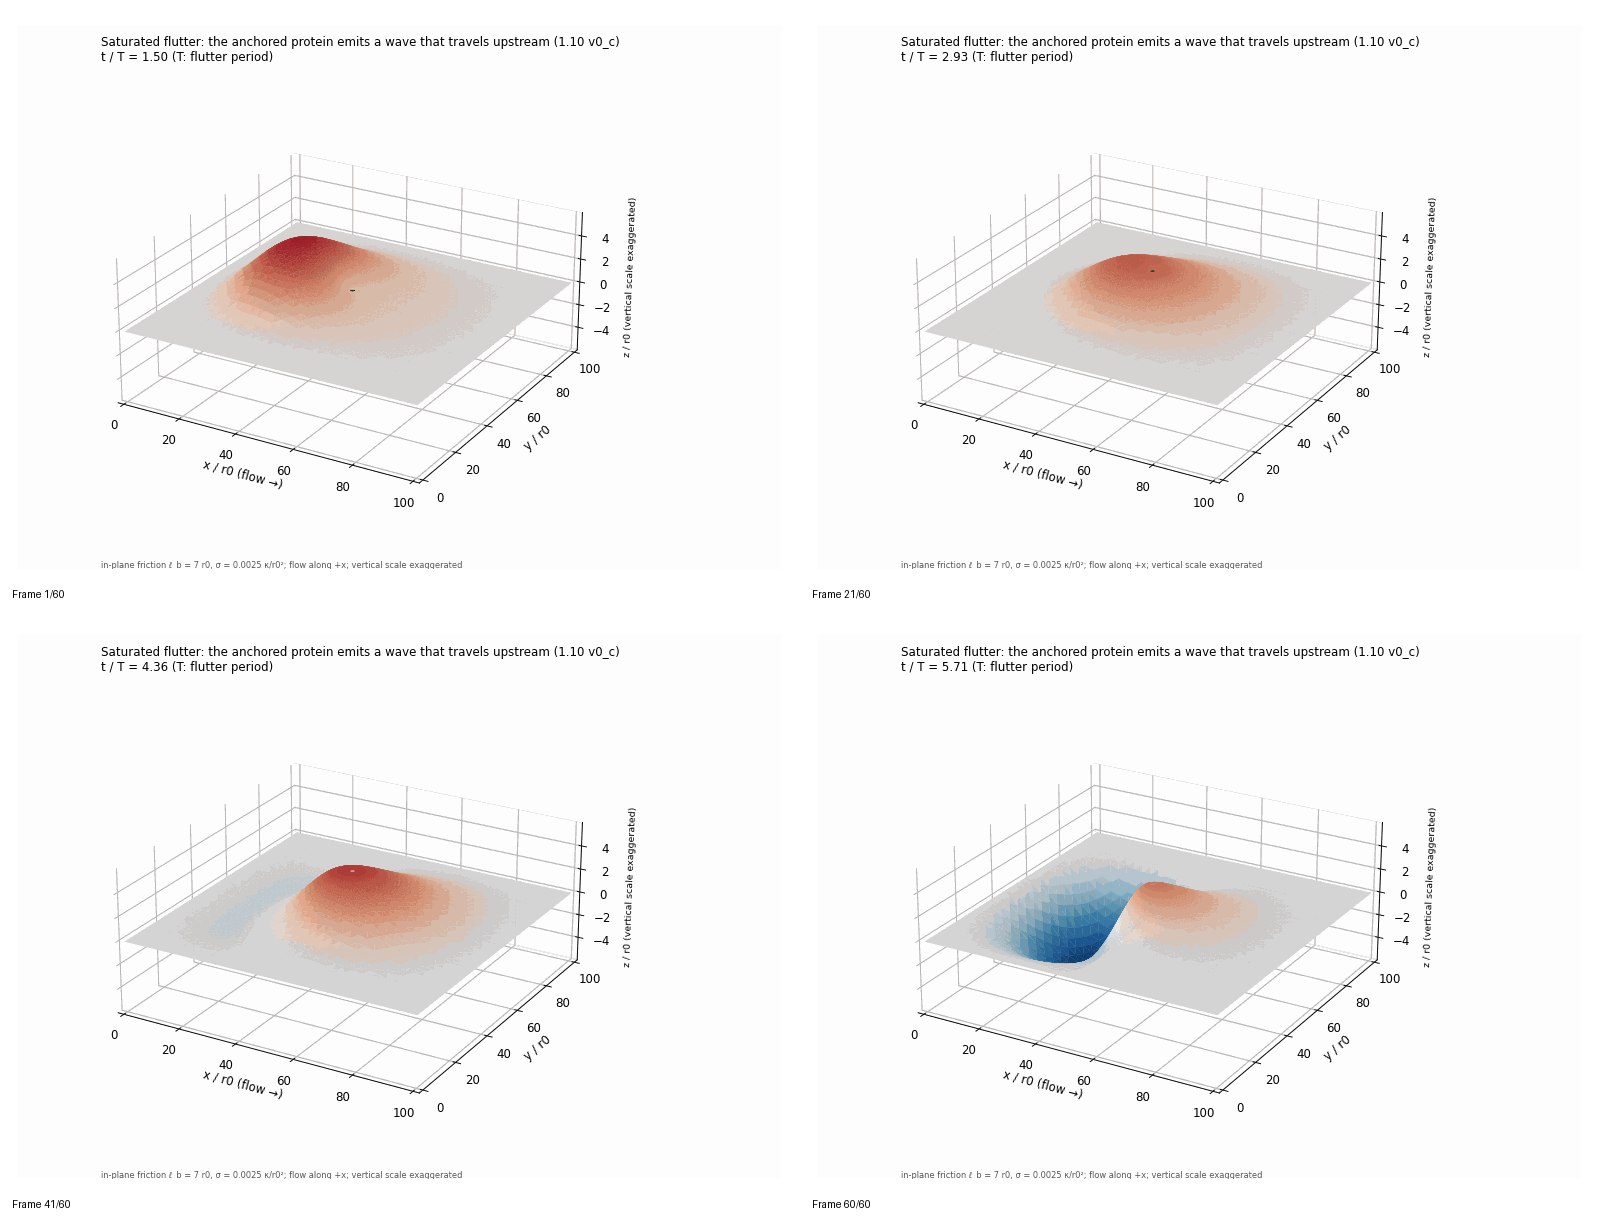
\includegraphics[width=\linewidth,height=170mm,keepaspectratio]{animation_stills/membrane_gif11_flutter_3d.png}\captionof{figure}[Archived figure]{Nonlinear friction-driven flutter: protein oscillation and a sustained source of upstream membrane waves. Four ordered frames are selected by frame index; spacing is not asserted to be uniform in physical time. \textit{Original GIF:} \path{research/membrane_stability/figures/gifs/gif11_flutter_3d.gif}. First added 2026-10-02.}\end{center}
\noindent\textit{Playback file in this source package:} \path{figures/membrane_gif11_flutter_3d.gif}.\clearpage
\begin{center}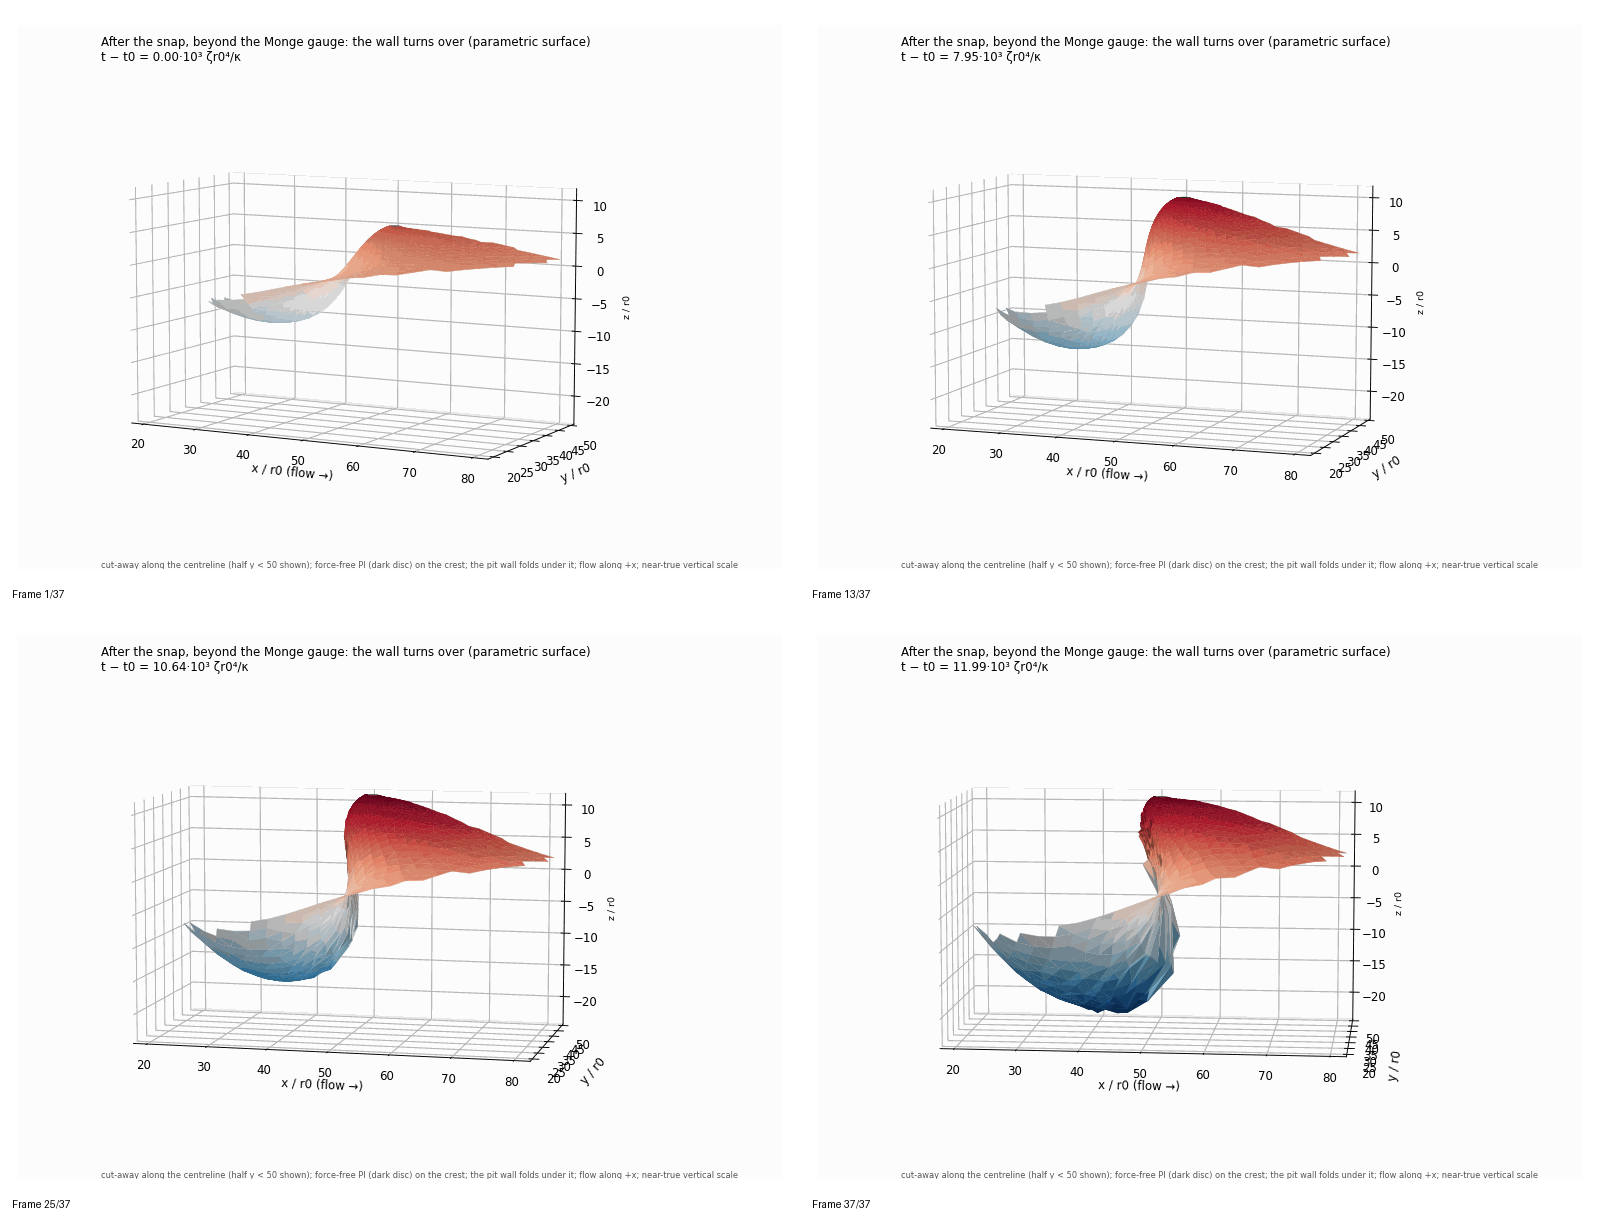
\includegraphics[width=\linewidth,height=170mm,keepaspectratio]{animation_stills/membrane_gif12_fold_parametric_3d.png}\captionof{figure}[Archived figure]{Parametric continuation of the force-free post-snap wall through vertical into an overhang underneath the lifted disc. The final state is distortion-limited. Four ordered frames are selected by frame index; spacing is not asserted to be uniform in physical time. \textit{Original GIF:} \path{research/membrane_stability/figures/gifs/gif12_fold_parametric_3d.gif}. First added 2026-10-02.}\end{center}
\noindent\textit{Playback file in this source package:} \path{figures/membrane_gif12_fold_parametric_3d.gif}.\clearpage
\begin{center}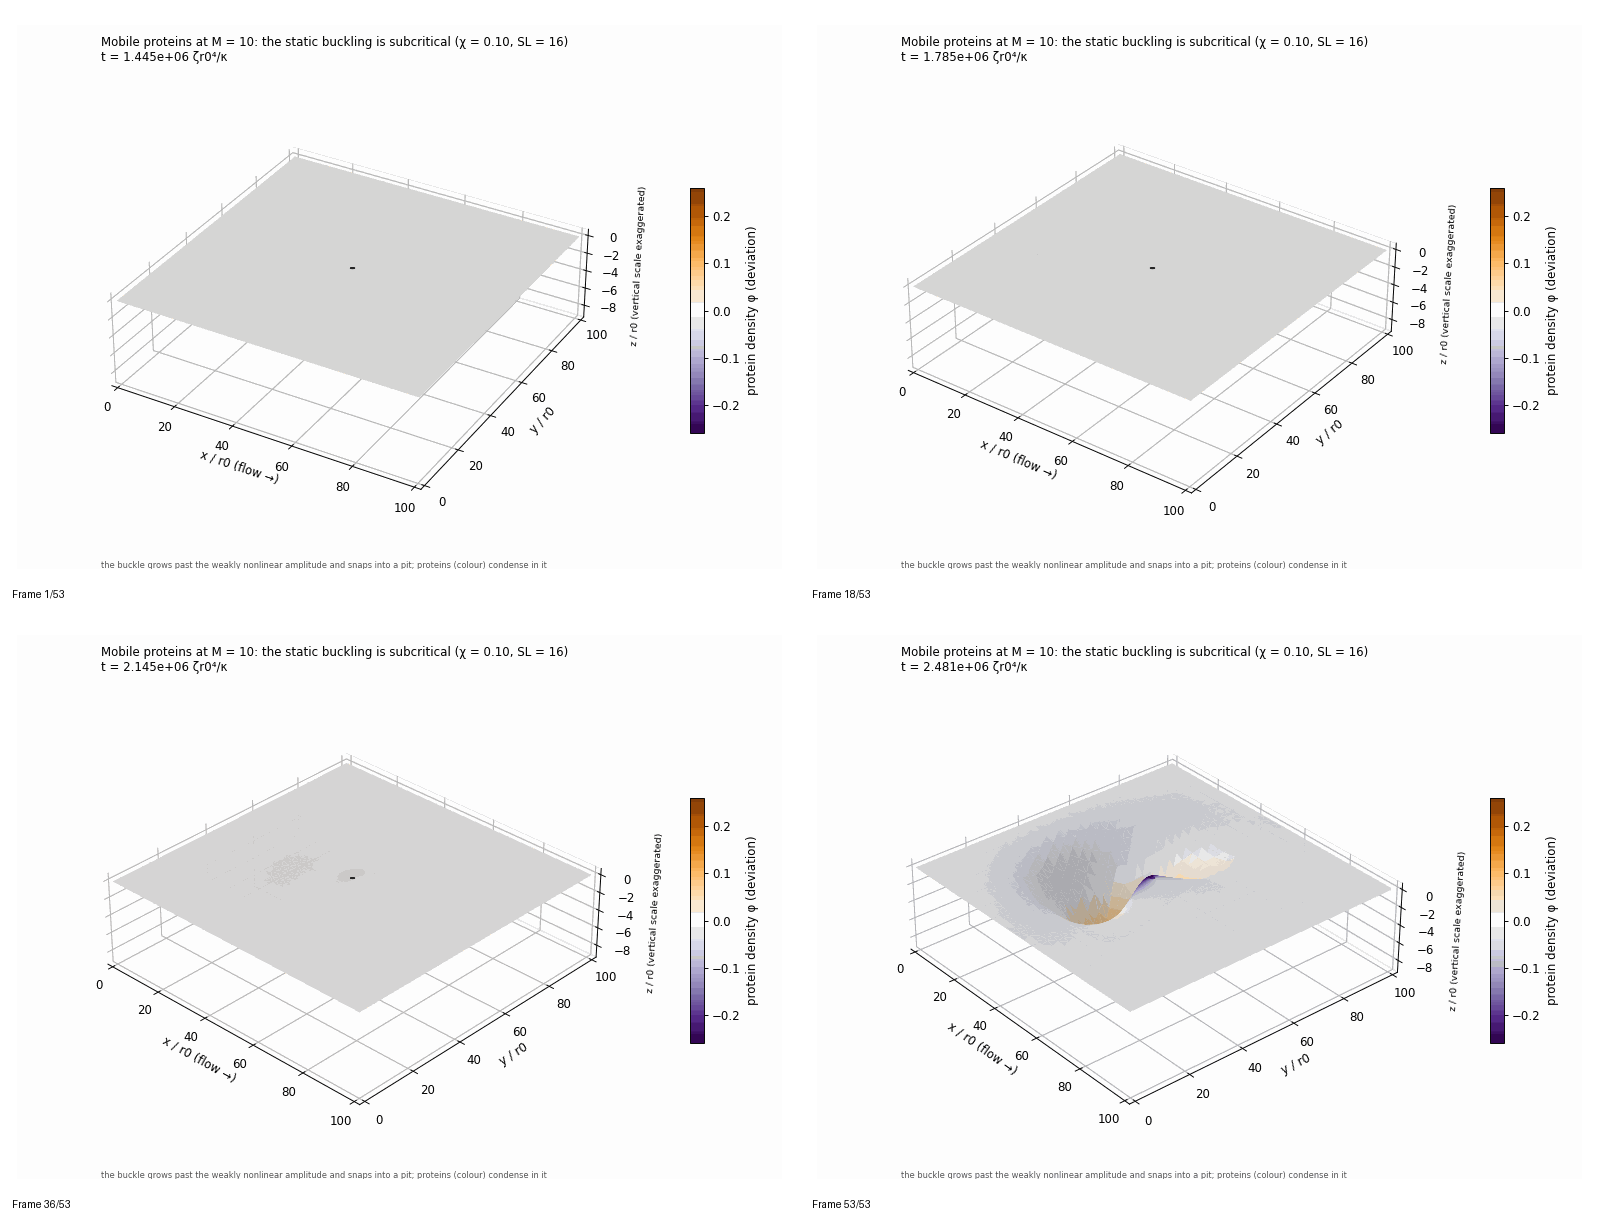
\includegraphics[width=\linewidth,height=170mm,keepaspectratio]{animation_stills/membrane_gif13_codim2_static_runaway_3d.png}\captionof{figure}[Archived figure]{Intermediate-mobility clamped-protein static-sector runaway. Shape and signed density deviation grow into a deep pit; no terminal attractor is resolved. Four ordered frames are selected by frame index; spacing is not asserted to be uniform in physical time. \textit{Original GIF:} \path{research/membrane_stability/figures/gifs/gif13_codim2_static_runaway_3d.gif}. First added 2026-10-03.}\end{center}
\noindent\textit{Playback file in this source package:} \path{figures/membrane_gif13_codim2_static_runaway_3d.gif}.\clearpage
\begin{center}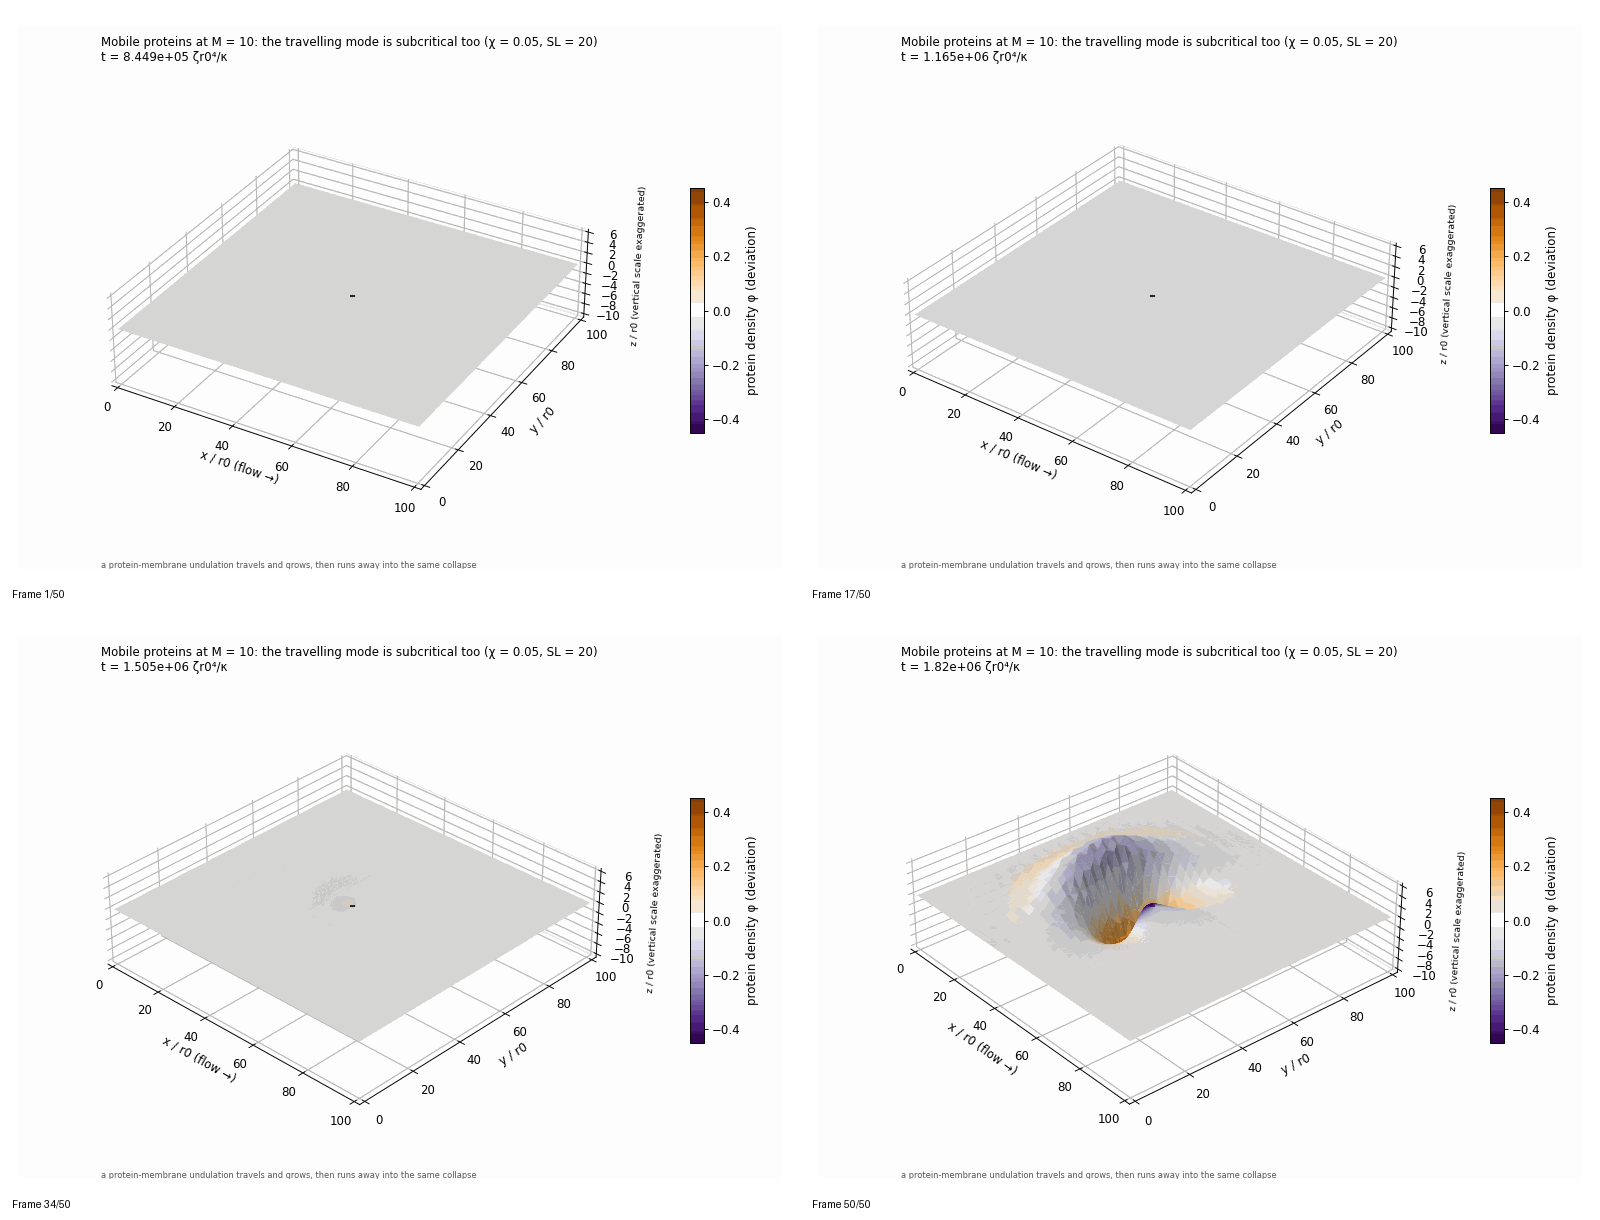
\includegraphics[width=\linewidth,height=170mm,keepaspectratio]{animation_stills/membrane_gif14_codim2_oscillatory_3d.png}\captionof{figure}[Archived figure]{Intermediate-mobility oscillatory-sector runaway. A growing travelling mode evolves into collapse rather than a saturated wave source. Four ordered frames are selected by frame index; spacing is not asserted to be uniform in physical time. \textit{Original GIF:} \path{research/membrane_stability/figures/gifs/gif14_codim2_oscillatory_3d.gif}. First added 2026-10-03.}\end{center}
\noindent\textit{Playback file in this source package:} \path{figures/membrane_gif14_codim2_oscillatory_3d.gif}.\clearpage
\begin{center}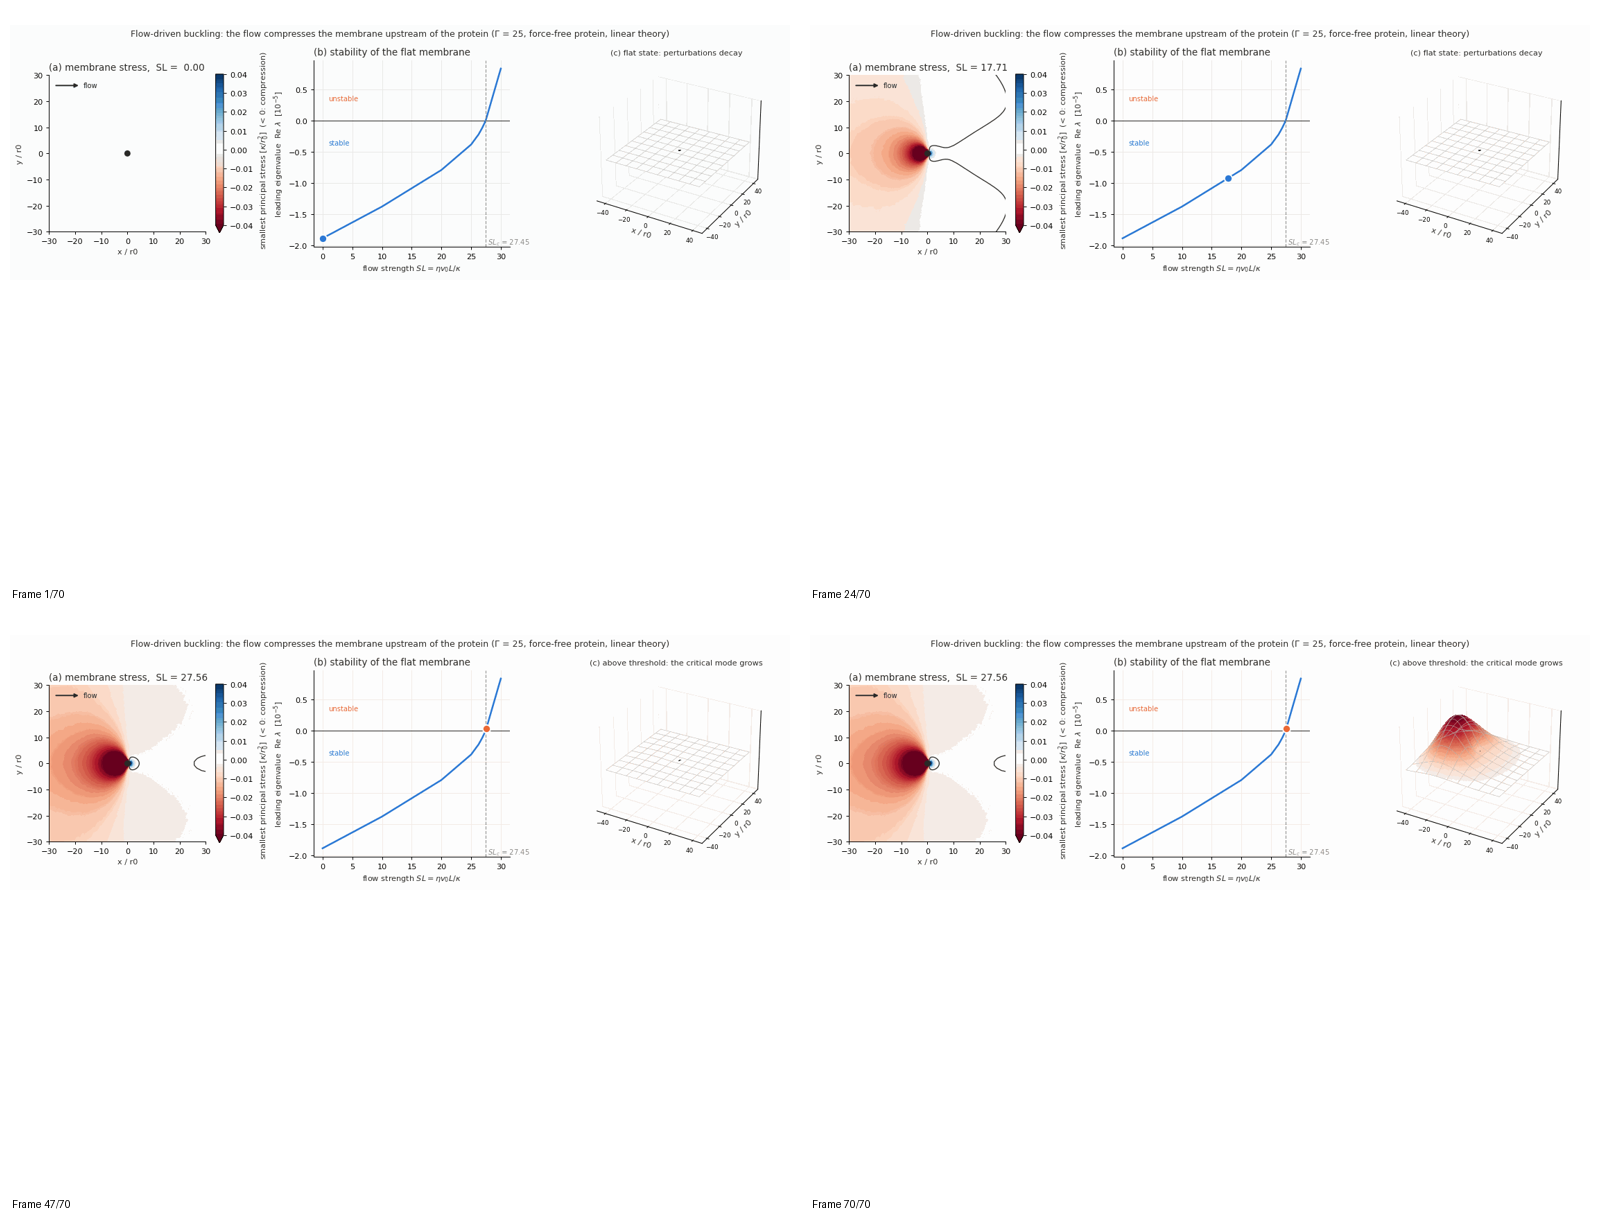
\includegraphics[width=\linewidth,height=170mm,keepaspectratio]{animation_stills/membrane_gif1_flow_buckling_onset.png}\captionof{figure}[Archived figure]{Critical-mode visualization of flow-driven buckling and upstream compression. This onset sequence belongs to the corrected study's visualization workflow; the static plots and force condition supply the quantitative threshold. Four ordered frames are selected by frame index; spacing is not asserted to be uniform in physical time. \textit{Original GIF:} \path{research/membrane_stability/figures/gifs/gif1_flow_buckling_onset.gif}. First added 2026-09-30.}\end{center}
\noindent\textit{Playback file in this source package:} \path{figures/membrane_gif1_flow_buckling_onset.gif}.\clearpage
\begin{center}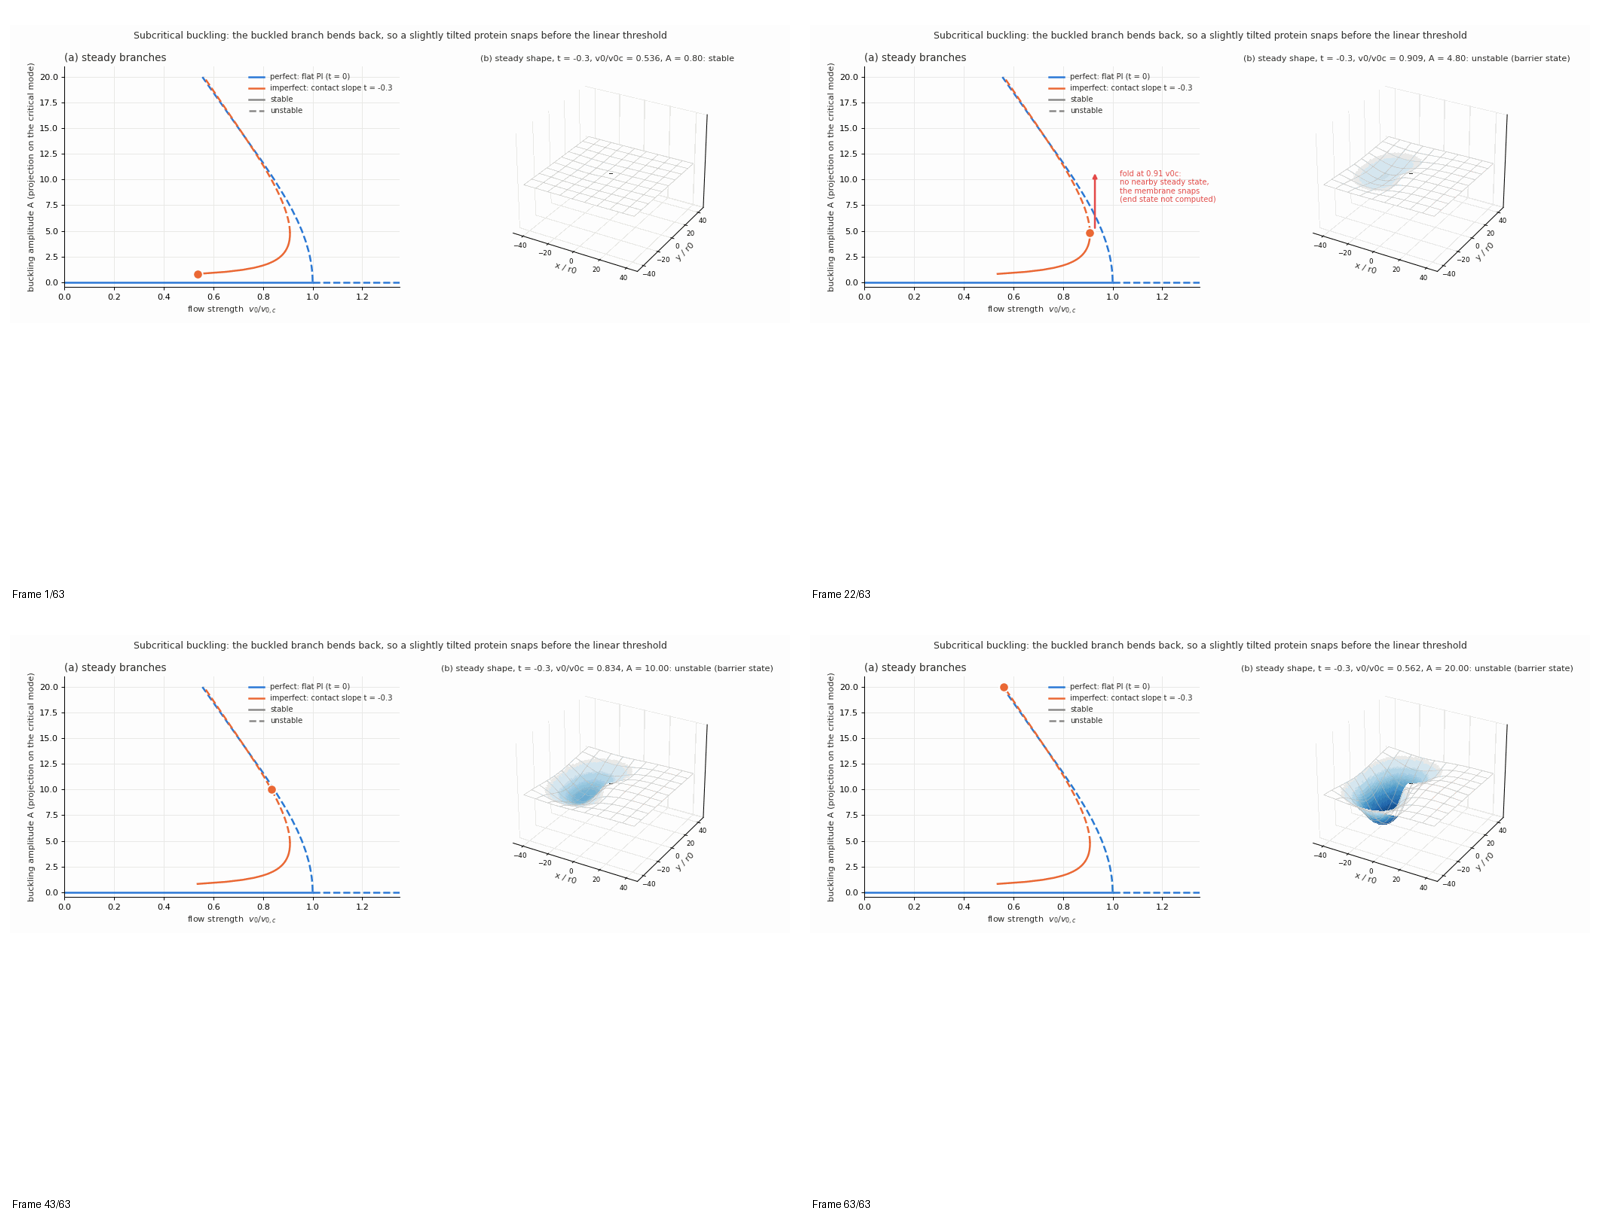
\includegraphics[width=\linewidth,height=170mm,keepaspectratio]{animation_stills/membrane_gif2_subcritical_snap.png}\captionof{figure}[Archived figure]{Branch visualization of the subcritical snap and its imperfection-sensitive fold. A continuation animation is a sequence of equilibria, not a physical-time simulation. Four ordered frames are selected by frame index; spacing is not asserted to be uniform in physical time. \textit{Original GIF:} \path{research/membrane_stability/figures/gifs/gif2_subcritical_snap.gif}. First added 2026-09-30.}\end{center}
\noindent\textit{Playback file in this source package:} \path{figures/membrane_gif2_subcritical_snap.gif}.\clearpage
\begin{center}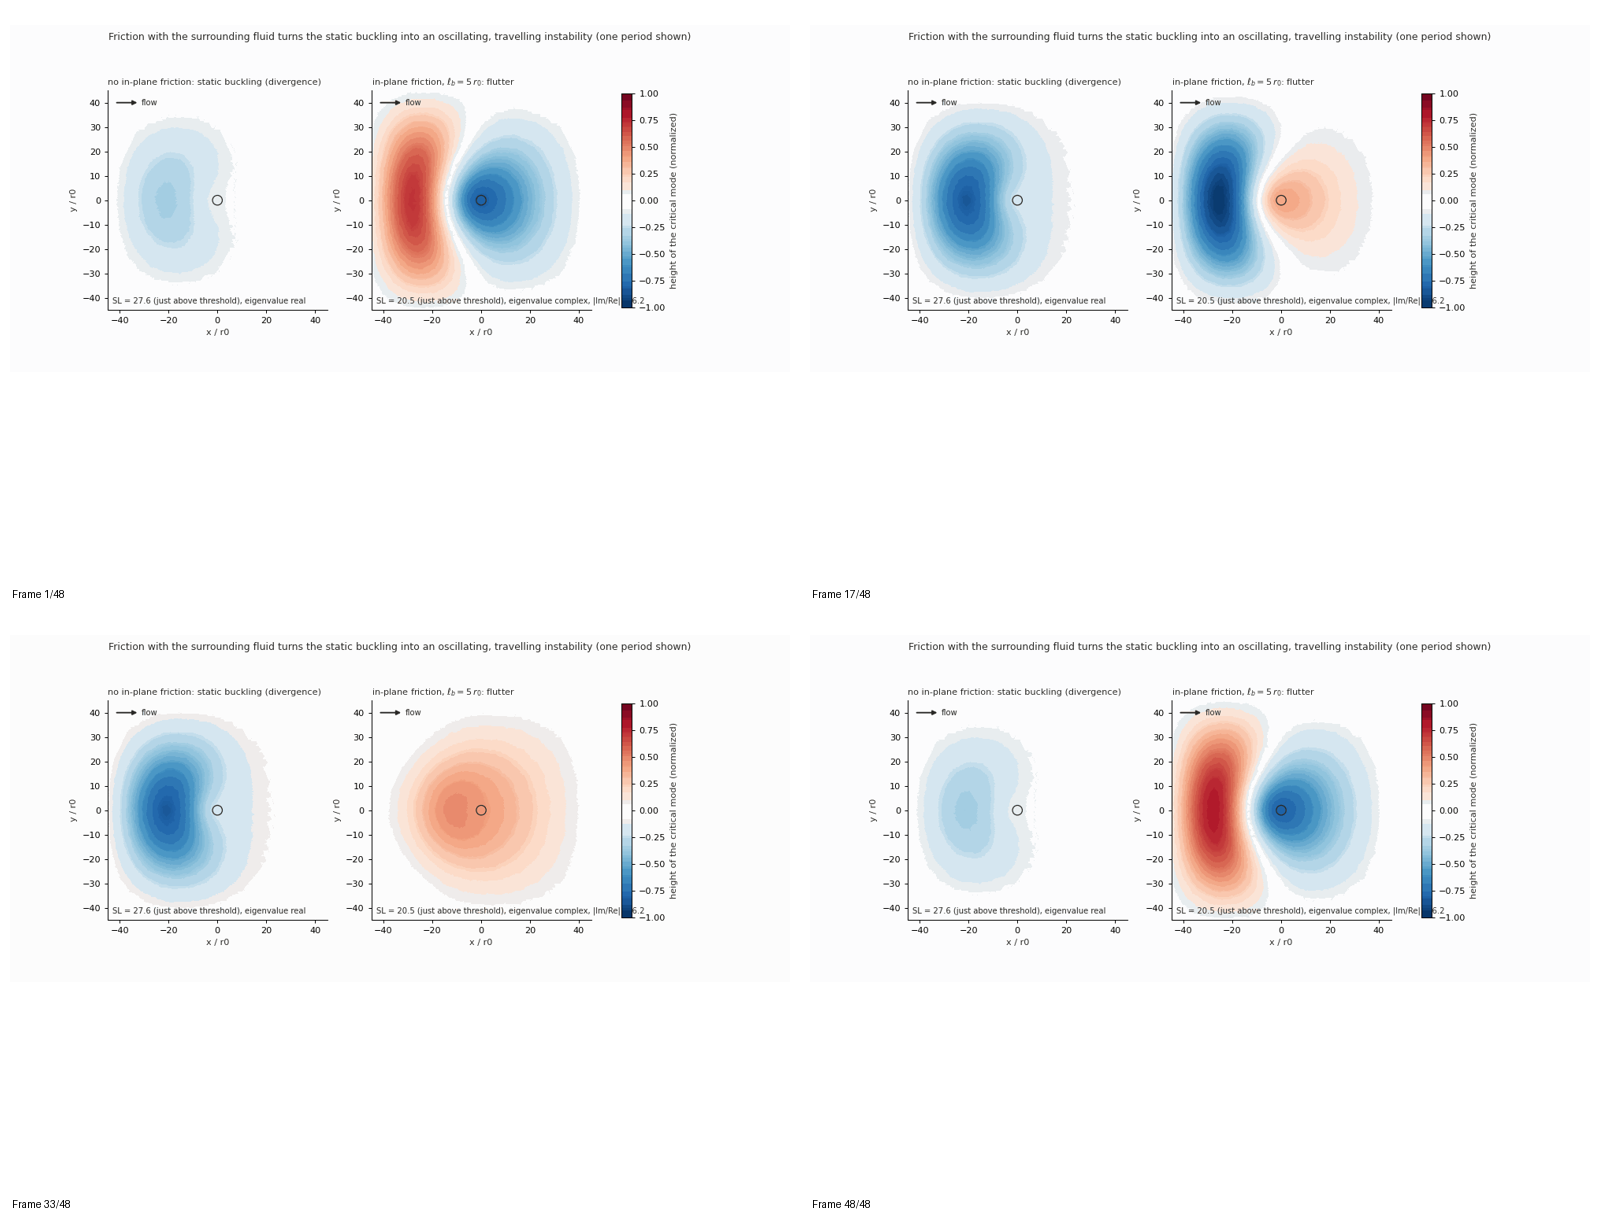
\includegraphics[width=\linewidth,height=170mm,keepaspectratio]{animation_stills/membrane_gif3_divergence_vs_flutter.png}\captionof{figure}[Archived figure]{Real divergence mode versus oscillatory flutter mode. The travelling phase of the complex mode is distinct from a nonlinear saturated cycle. Four ordered frames are selected by frame index; spacing is not asserted to be uniform in physical time. \textit{Original GIF:} \path{research/membrane_stability/figures/gifs/gif3_divergence_vs_flutter.gif}. First added 2026-09-30.}\end{center}
\noindent\textit{Playback file in this source package:} \path{figures/membrane_gif3_divergence_vs_flutter.gif}.\clearpage
\begin{center}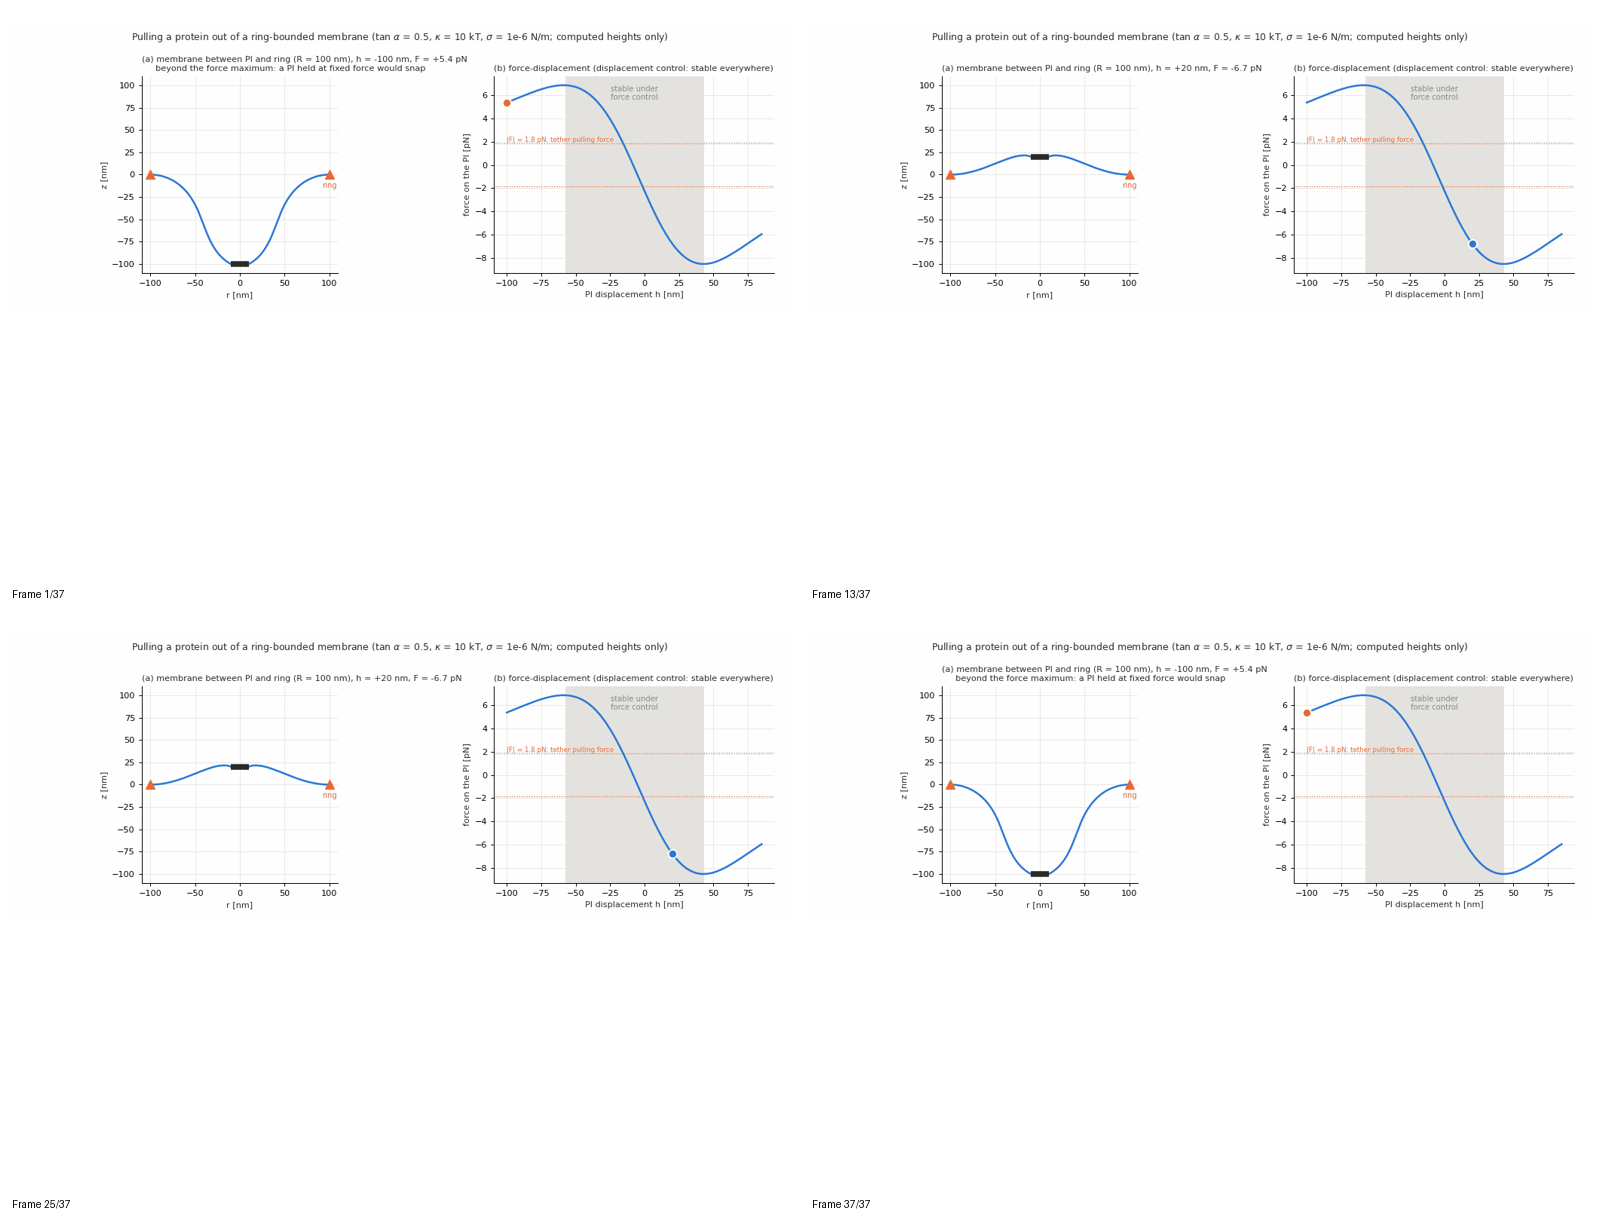
\includegraphics[width=\linewidth,height=170mm,keepaspectratio]{animation_stills/membrane_gif4_ring_pulling.png}\captionof{figure}[Archived figure]{Ring-pulling profile sequence. The imposed height varies along a branch; force-control stability is determined separately by the virtual-work stiffness. Four ordered frames are selected by frame index; spacing is not asserted to be uniform in physical time. \textit{Original GIF:} \path{research/membrane_stability/figures/gifs/gif4_ring_pulling.gif}. First added 2026-09-30.}\end{center}
\noindent\textit{Playback file in this source package:} \path{figures/membrane_gif4_ring_pulling.gif}.\clearpage
\begin{center}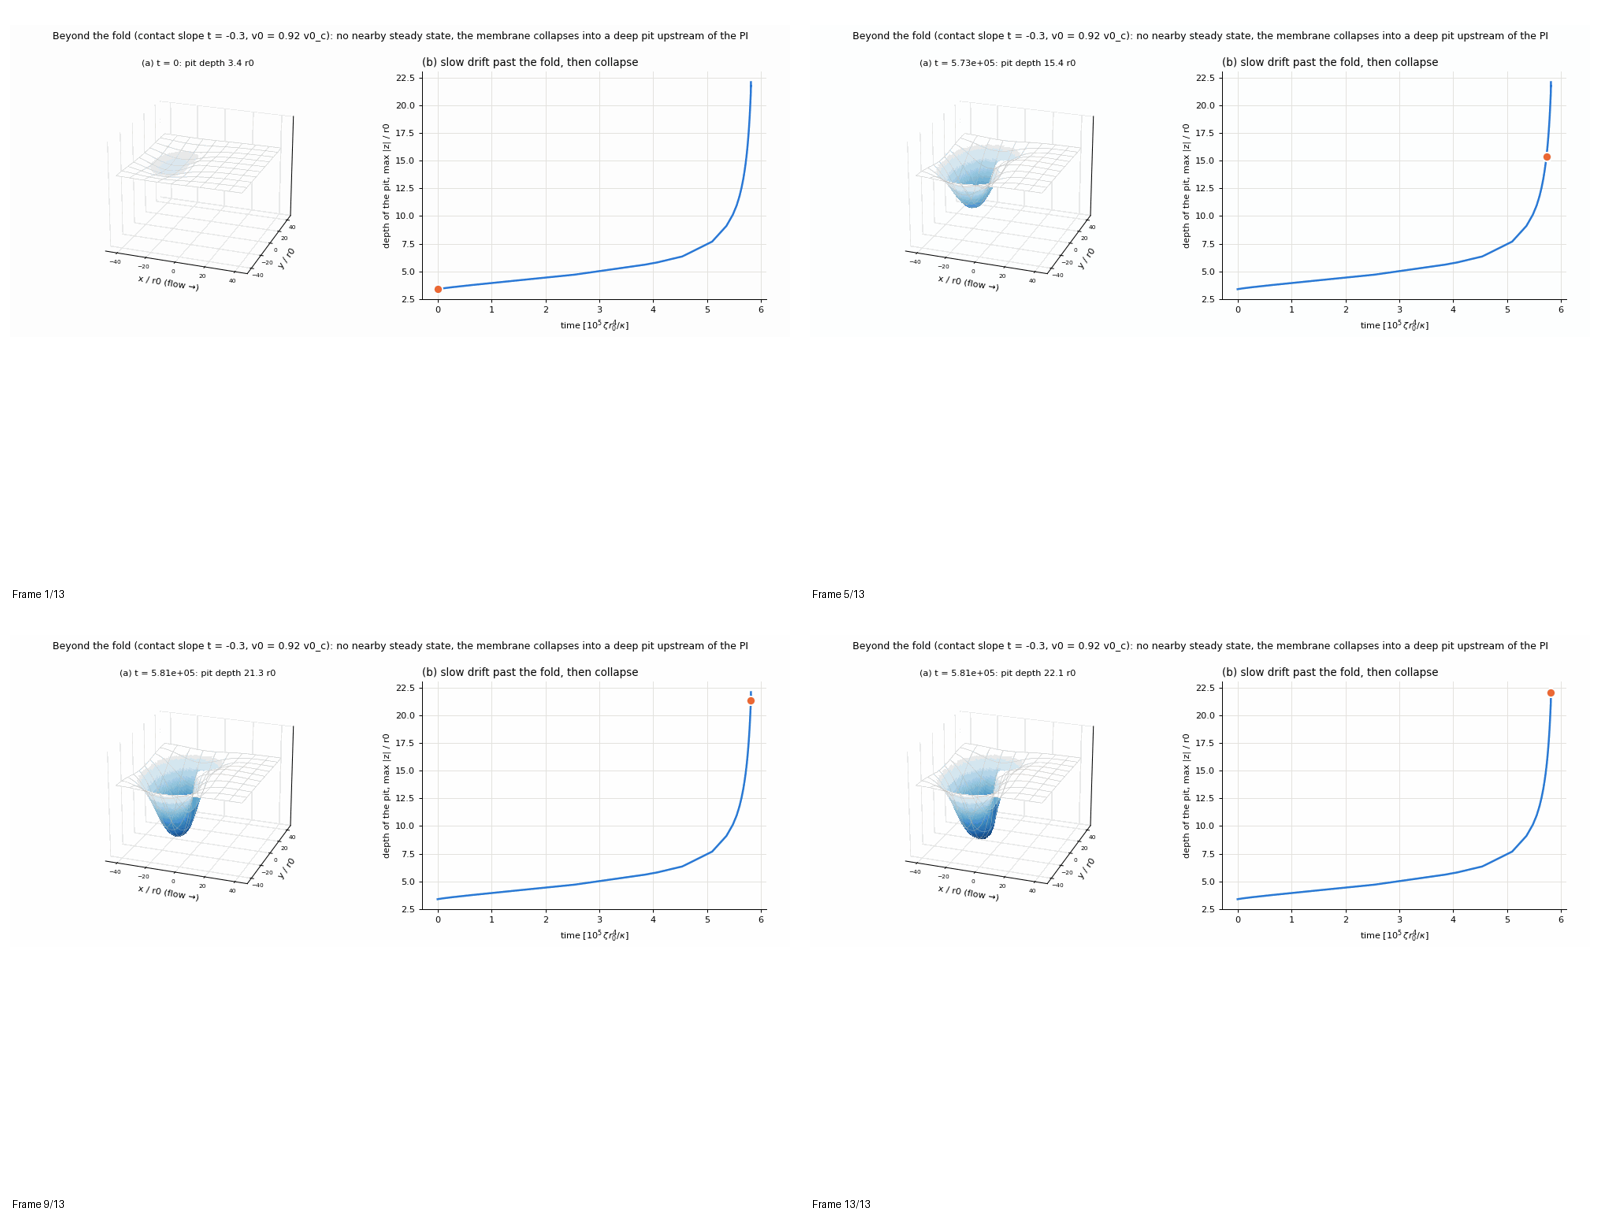
\includegraphics[width=\linewidth,height=170mm,keepaspectratio]{animation_stills/membrane_gif5_post_snap_collapse.png}\captionof{figure}[Archived figure]{Clamped-protein post-fold time integration: an upstream pit grows and the wall approaches vertical. Four ordered frames are selected by frame index; spacing is not asserted to be uniform in physical time. \textit{Original GIF:} \path{research/membrane_stability/figures/gifs/gif5_post_snap_collapse.gif}. First added 2026-10-01.}\end{center}
\noindent\textit{Playback file in this source package:} \path{figures/membrane_gif5_post_snap_collapse.gif}.\clearpage
\begin{center}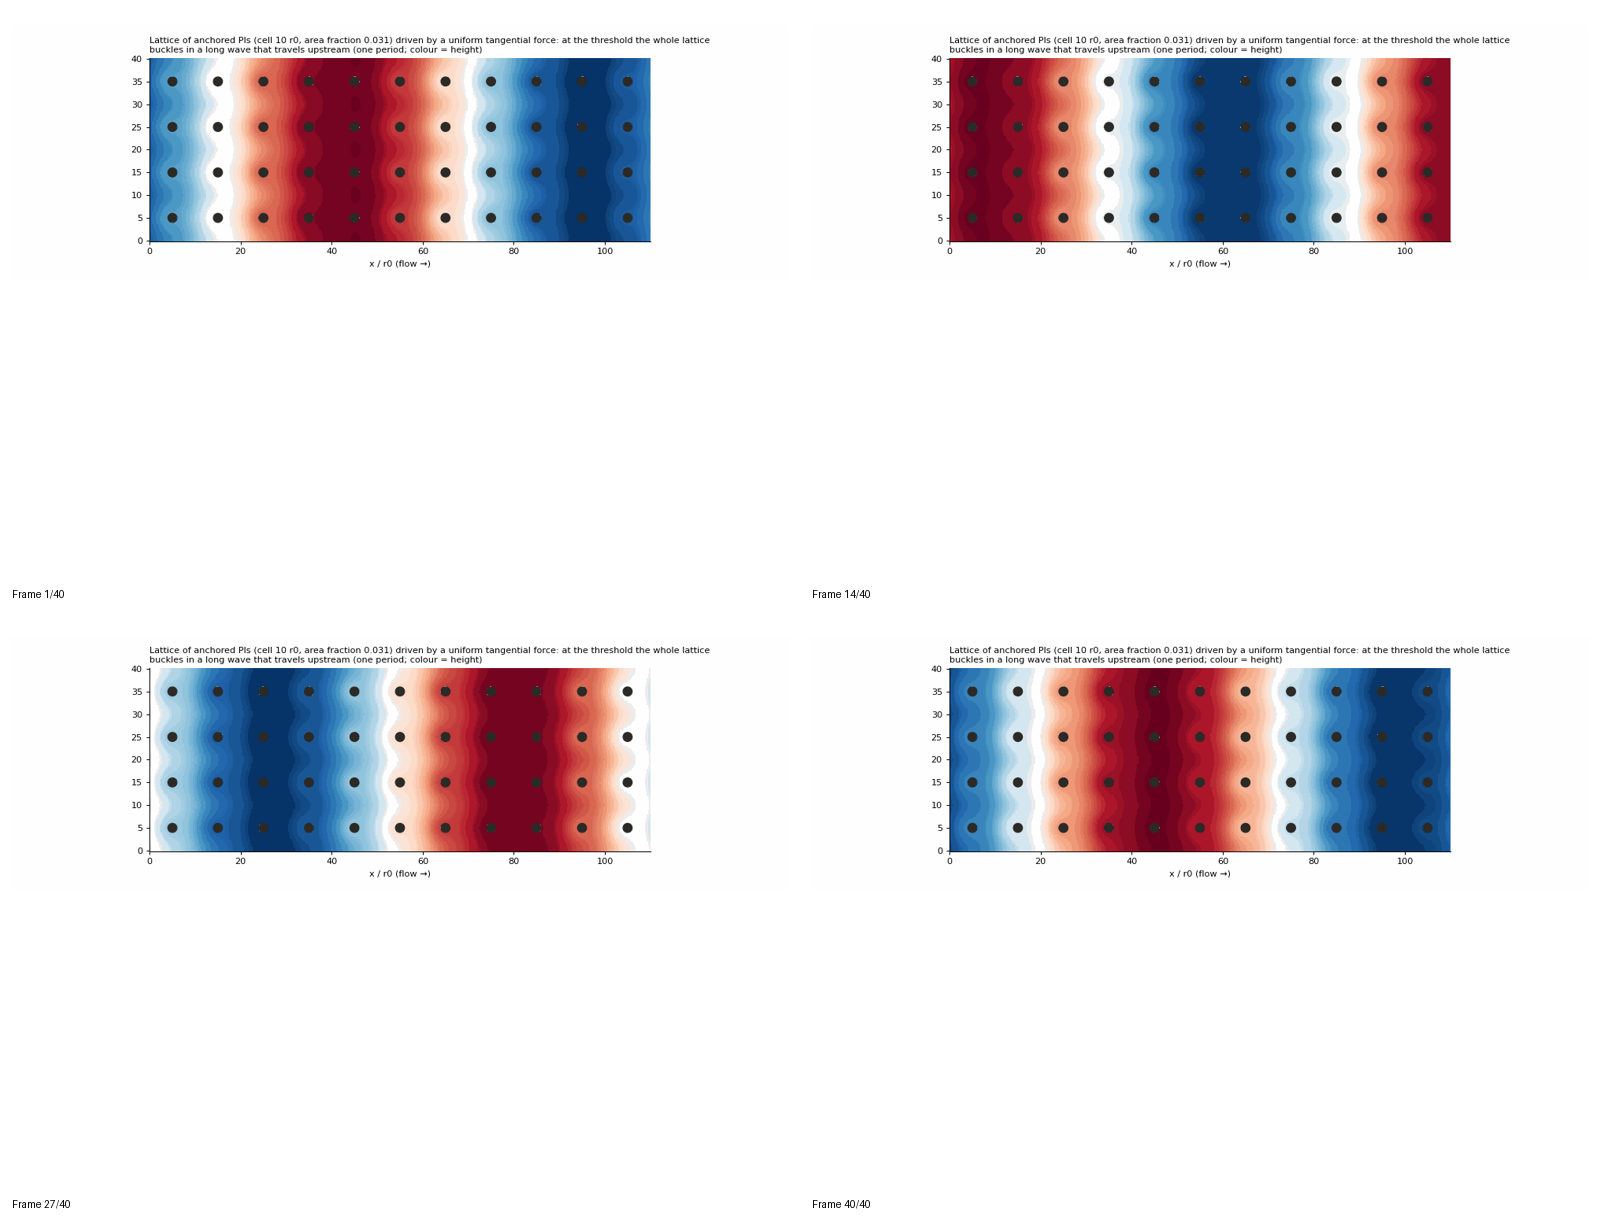
\includegraphics[width=\linewidth,height=170mm,keepaspectratio]{animation_stills/membrane_gif6_lattice_wave.png}\captionof{figure}[Archived figure]{Collective Bloch-wave pattern of a periodic protein array. This visualizes the long-wave instability and upstream phase drift, not a nonlinear terrace simulation. Four ordered frames are selected by frame index; spacing is not asserted to be uniform in physical time. \textit{Original GIF:} \path{research/membrane_stability/figures/gifs/gif6_lattice_wave.gif}. First added 2026-10-01.}\end{center}
\noindent\textit{Playback file in this source package:} \path{figures/membrane_gif6_lattice_wave.gif}.\clearpage
\begin{center}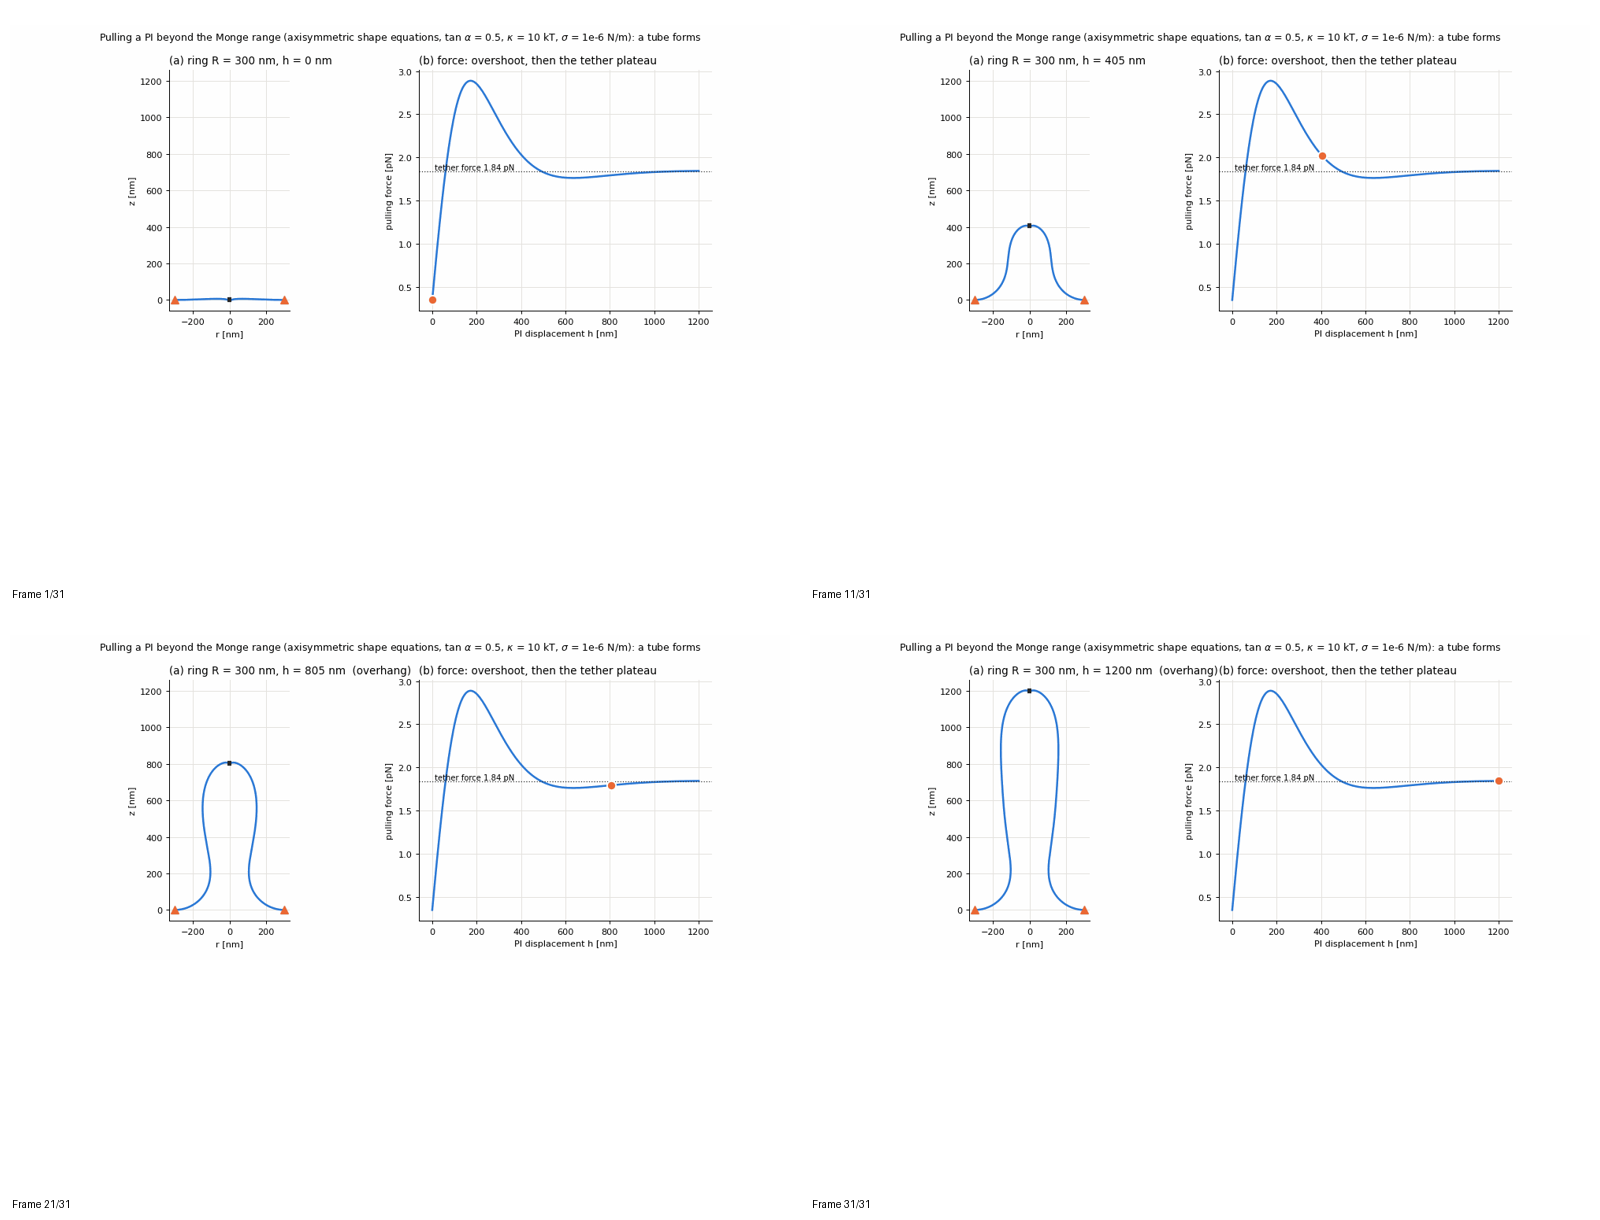
\includegraphics[width=\linewidth,height=170mm,keepaspectratio]{animation_stills/membrane_gif7_tube_extrusion.png}\captionof{figure}[Archived figure]{No-flow axisymmetric tube/neck continuation beyond the Monge range. The force plateau for a large ring agrees with tether theory. Four ordered frames are selected by frame index; spacing is not asserted to be uniform in physical time. \textit{Original GIF:} \path{research/membrane_stability/figures/gifs/gif7_tube_extrusion.gif}. First added 2026-10-01.}\end{center}
\noindent\textit{Playback file in this source package:} \path{figures/membrane_gif7_tube_extrusion.gif}.\clearpage
\begin{center}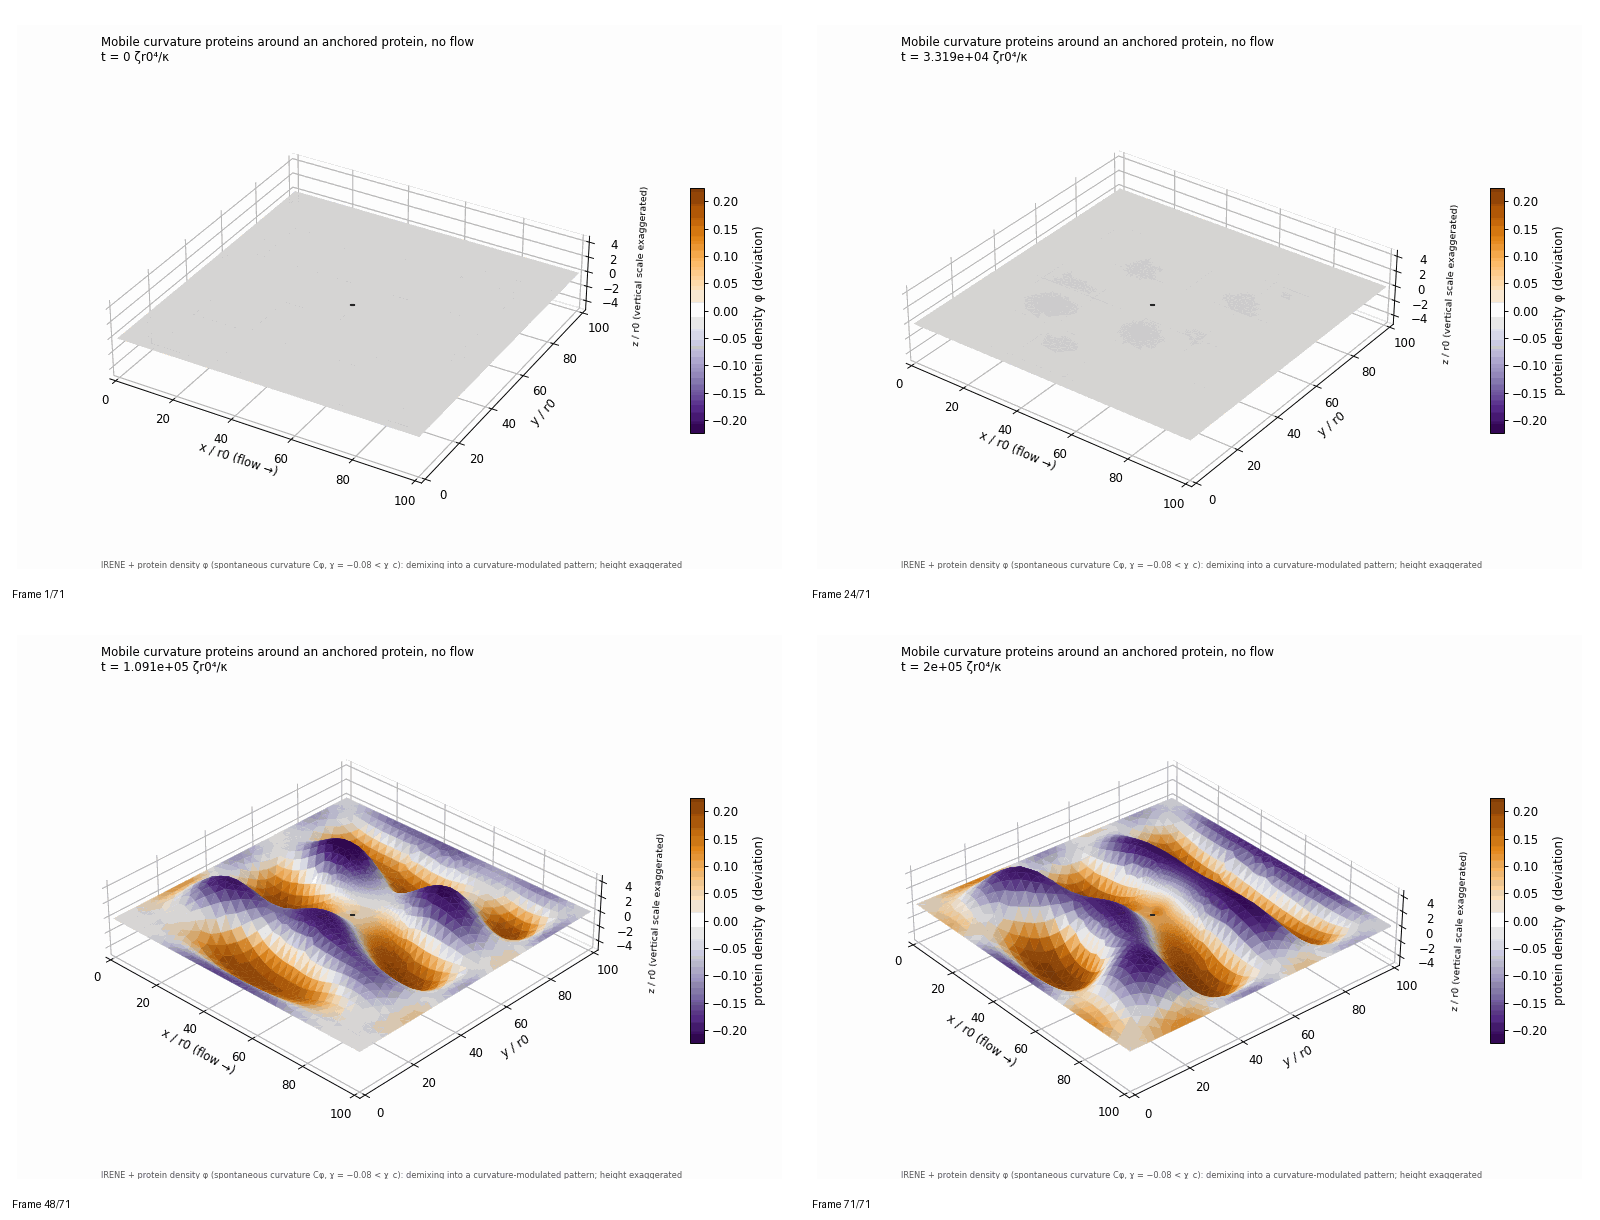
\includegraphics[width=\linewidth,height=170mm,keepaspectratio]{animation_stills/membrane_gif8_proteins_rest_3d.png}\captionof{figure}[Archived figure]{Consistent nonlinear curvature-protein demixing at rest. A modulated labyrinth forms while the free energy decreases. Four ordered frames are selected by frame index; spacing is not asserted to be uniform in physical time. \textit{Original GIF:} \path{research/membrane_stability/figures/gifs/gif8_proteins_rest_3d.gif}. First added 2026-10-02.}\end{center}
\noindent\textit{Playback file in this source package:} \path{figures/membrane_gif8_proteins_rest_3d.gif}.\clearpage
\begin{center}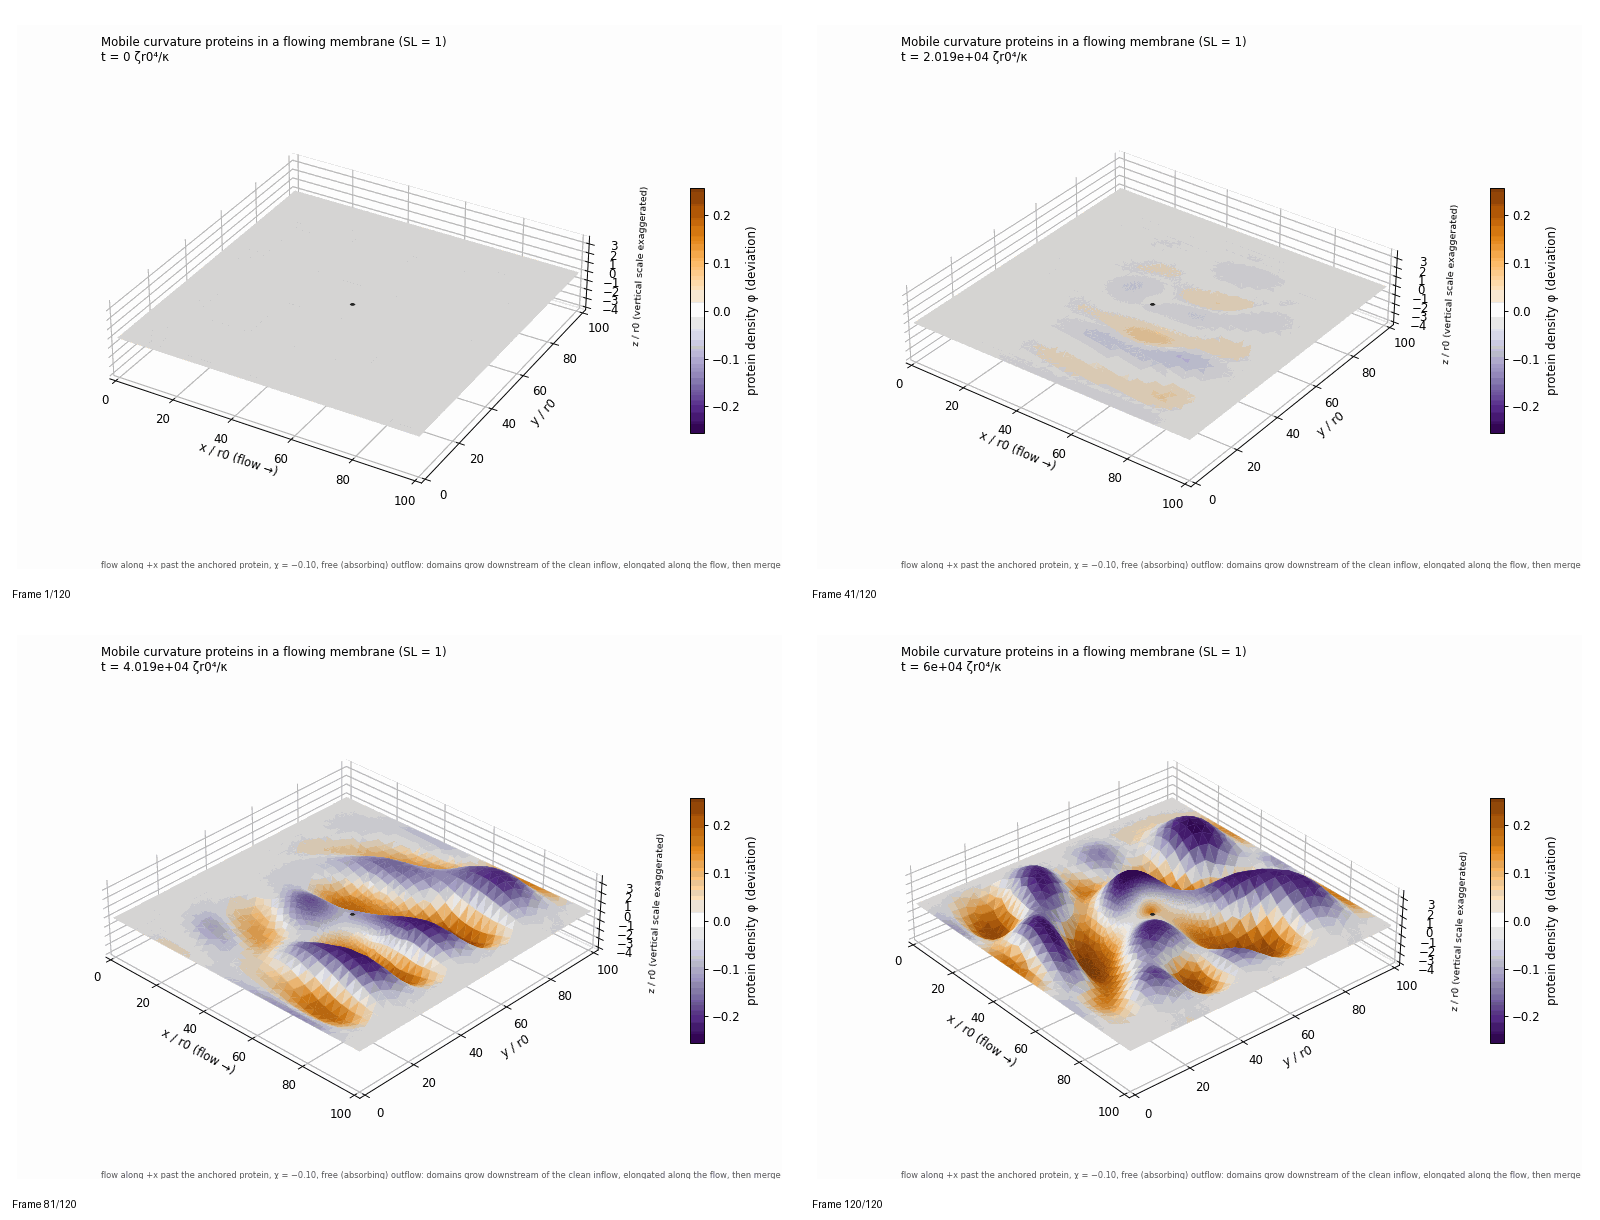
\includegraphics[width=\linewidth,height=170mm,keepaspectratio]{animation_stills/membrane_gif9_proteins_flow_3d.png}\captionof{figure}[Archived figure]{Mobile proteins in open flow. Downstream domains elongate along the flow and the membrane follows their curvature modulation. Four ordered frames are selected by frame index; spacing is not asserted to be uniform in physical time. \textit{Original GIF:} \path{research/membrane_stability/figures/gifs/gif9_proteins_flow_3d.gif}. First added 2026-10-02.}\end{center}
\noindent\textit{Playback file in this source package:} \path{figures/membrane_gif9_proteins_flow_3d.gif}.\clearpage

\clearpage
\section{Larger copies of main-text figures}
These figures repeat the main-text panels at the full available page width. Their interpretation and parameter qualifications are given in the corresponding main-text captions.
\begin{center}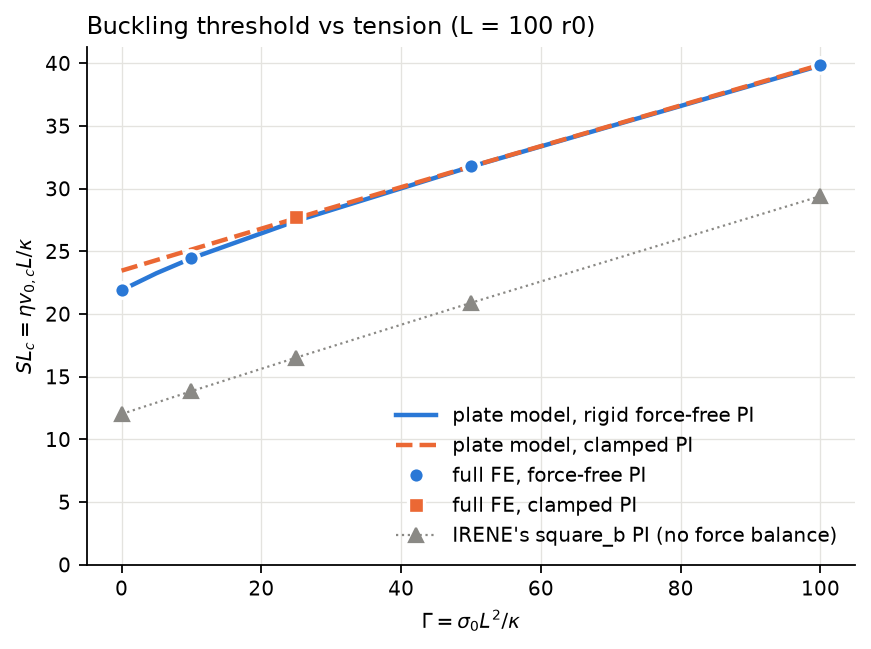
\includegraphics[width=\linewidth,height=175mm,keepaspectratio]{figures/membrane_flow2_threshold_vs_tension.png}\captionof{figure}[Main-text figure, larger copy]{Larger copy of main-text Figure 1. Consult its main-text caption for interpretation. \textit{Source:} \path{research/membrane_stability/figures/flow2_threshold_vs_tension.png}. First added 2026-09-30.}\end{center}\clearpage
\begin{center}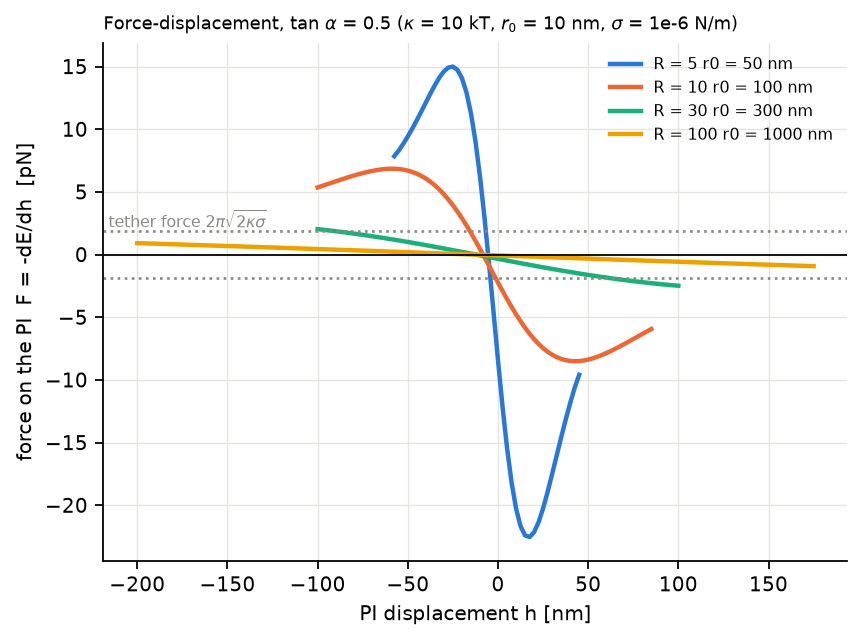
\includegraphics[width=\linewidth,height=175mm,keepaspectratio]{figures/membrane_ring_force_physical_units.png}\captionof{figure}[Main-text figure, larger copy]{Larger copy of main-text Figure 2. Consult its main-text caption for interpretation. \textit{Source:} \path{research/membrane_stability/figures/ring_force_physical_units.png}. First added 2026-09-30.}\end{center}\clearpage
\begin{center}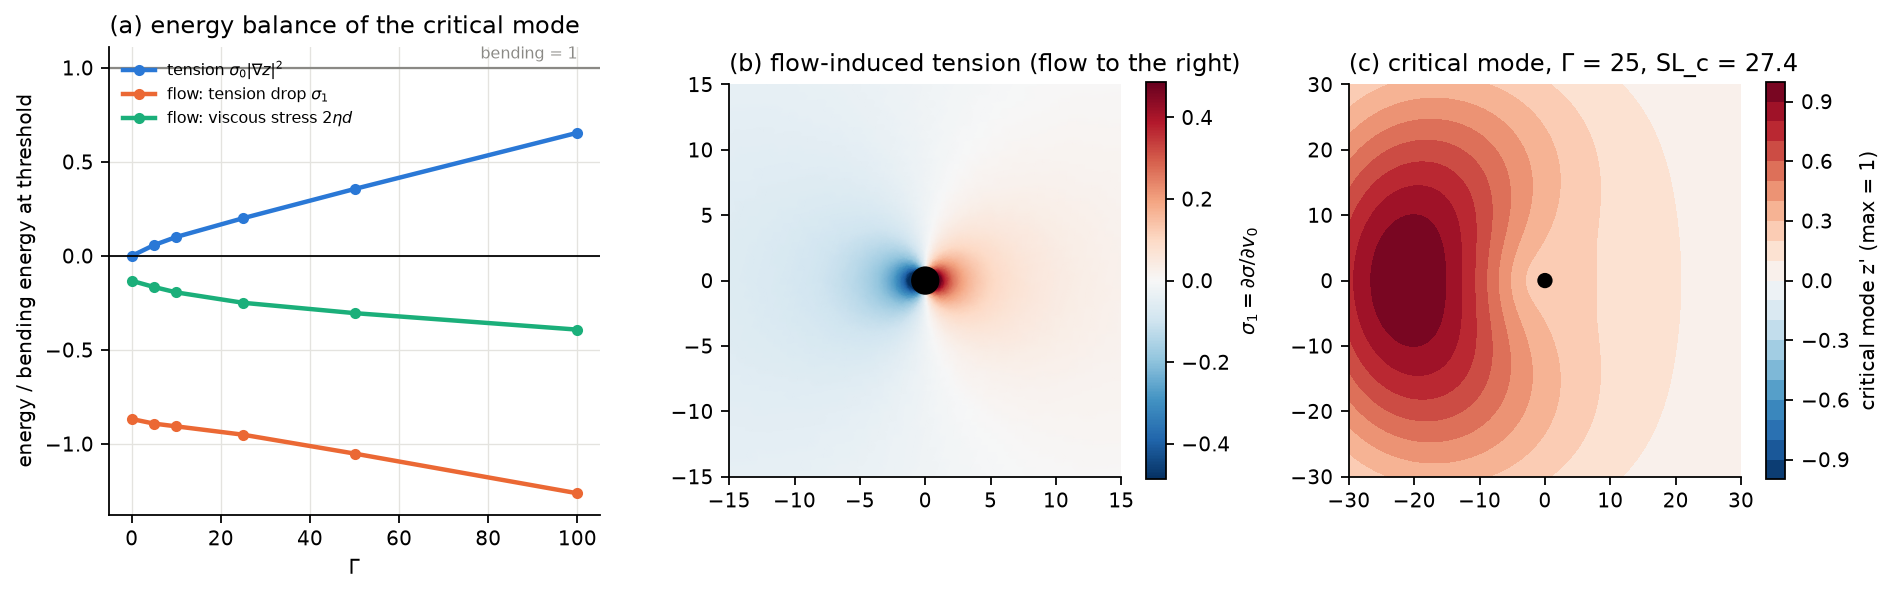
\includegraphics[width=\linewidth,height=175mm,keepaspectratio]{figures/membrane_flow2_plate_model.png}\captionof{figure}[Main-text figure, larger copy]{Larger copy of main-text Figure 3. Consult its main-text caption for interpretation. \textit{Source:} \path{research/membrane_stability/figures/flow2_plate_model.png}. First added 2026-09-30.}\end{center}\clearpage
\begin{center}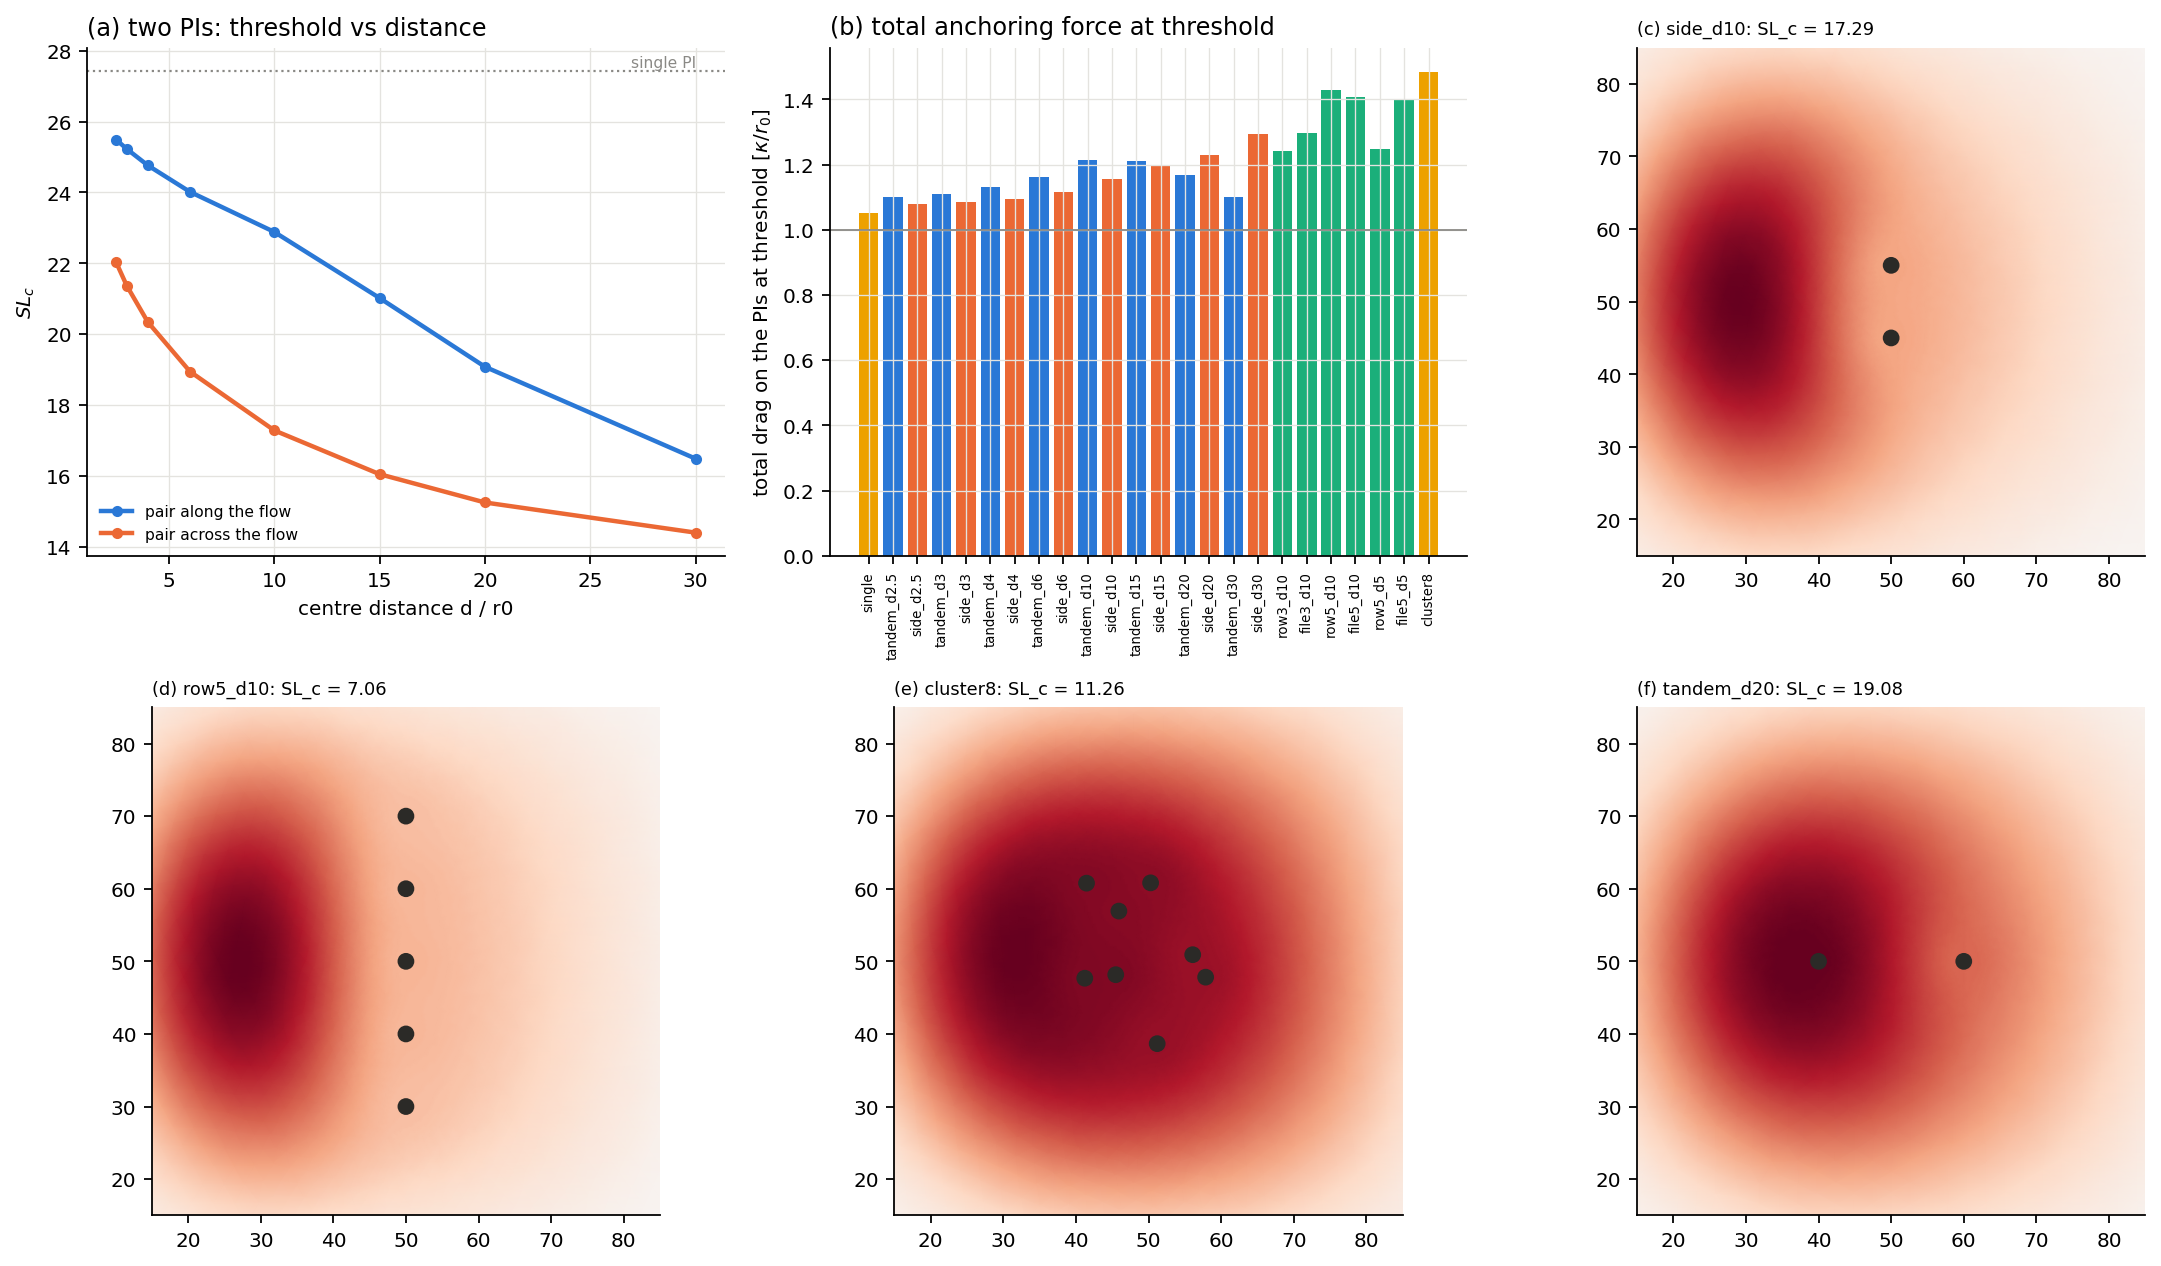
\includegraphics[width=\linewidth,height=175mm,keepaspectratio]{figures/membrane_r3_multi.png}\captionof{figure}[Main-text figure, larger copy]{Larger copy of main-text Figure 4. Consult its main-text caption for interpretation. \textit{Source:} \path{research/membrane_stability/figures/r3_multi.png}. First added 2026-10-01.}\end{center}\clearpage
\begin{center}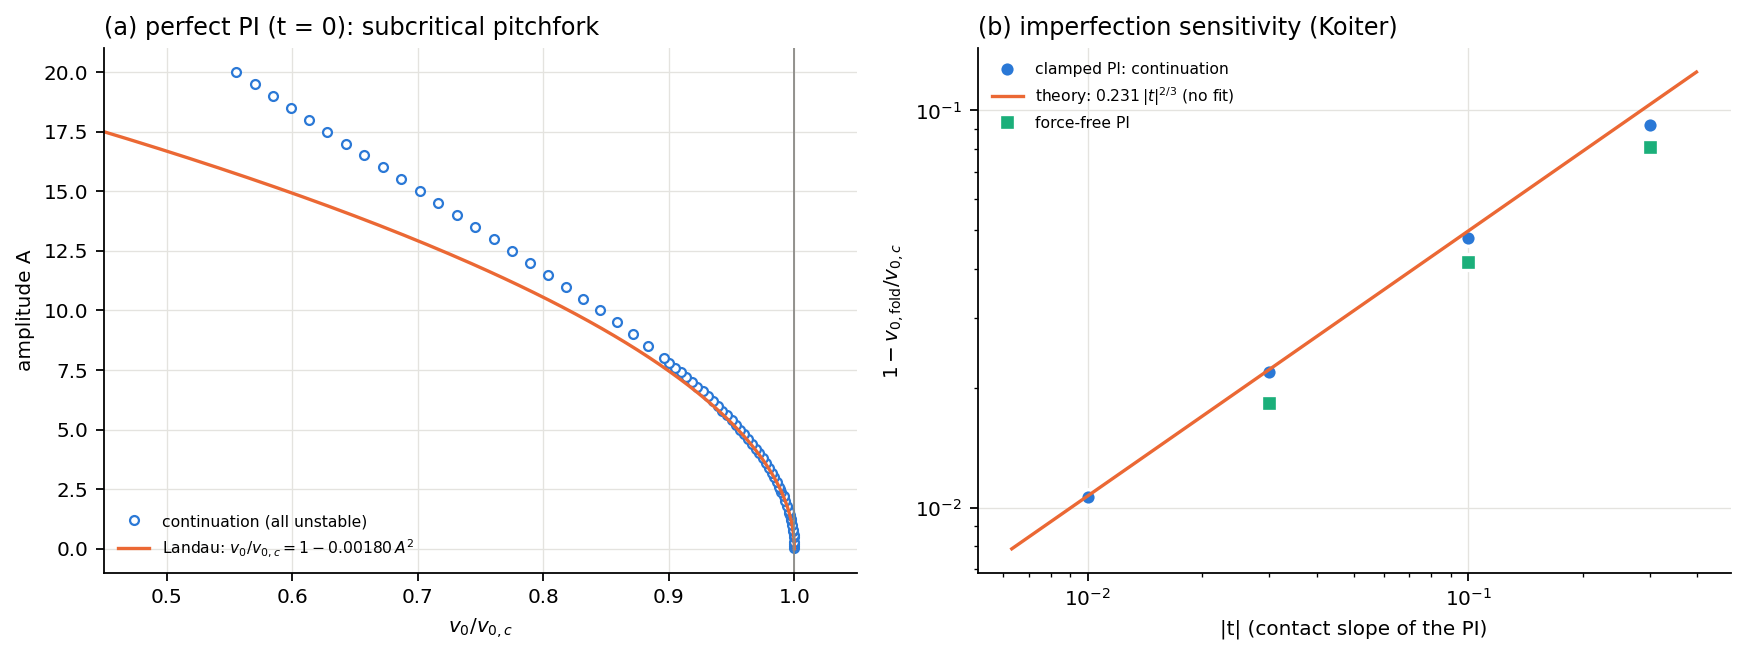
\includegraphics[width=\linewidth,height=175mm,keepaspectratio]{figures/membrane_r3_landau.png}\captionof{figure}[Main-text figure, larger copy]{Larger copy of main-text Figure 5. Consult its main-text caption for interpretation. \textit{Source:} \path{research/membrane_stability/figures/r3_landau.png}. First added 2026-10-01.}\end{center}\clearpage
\begin{center}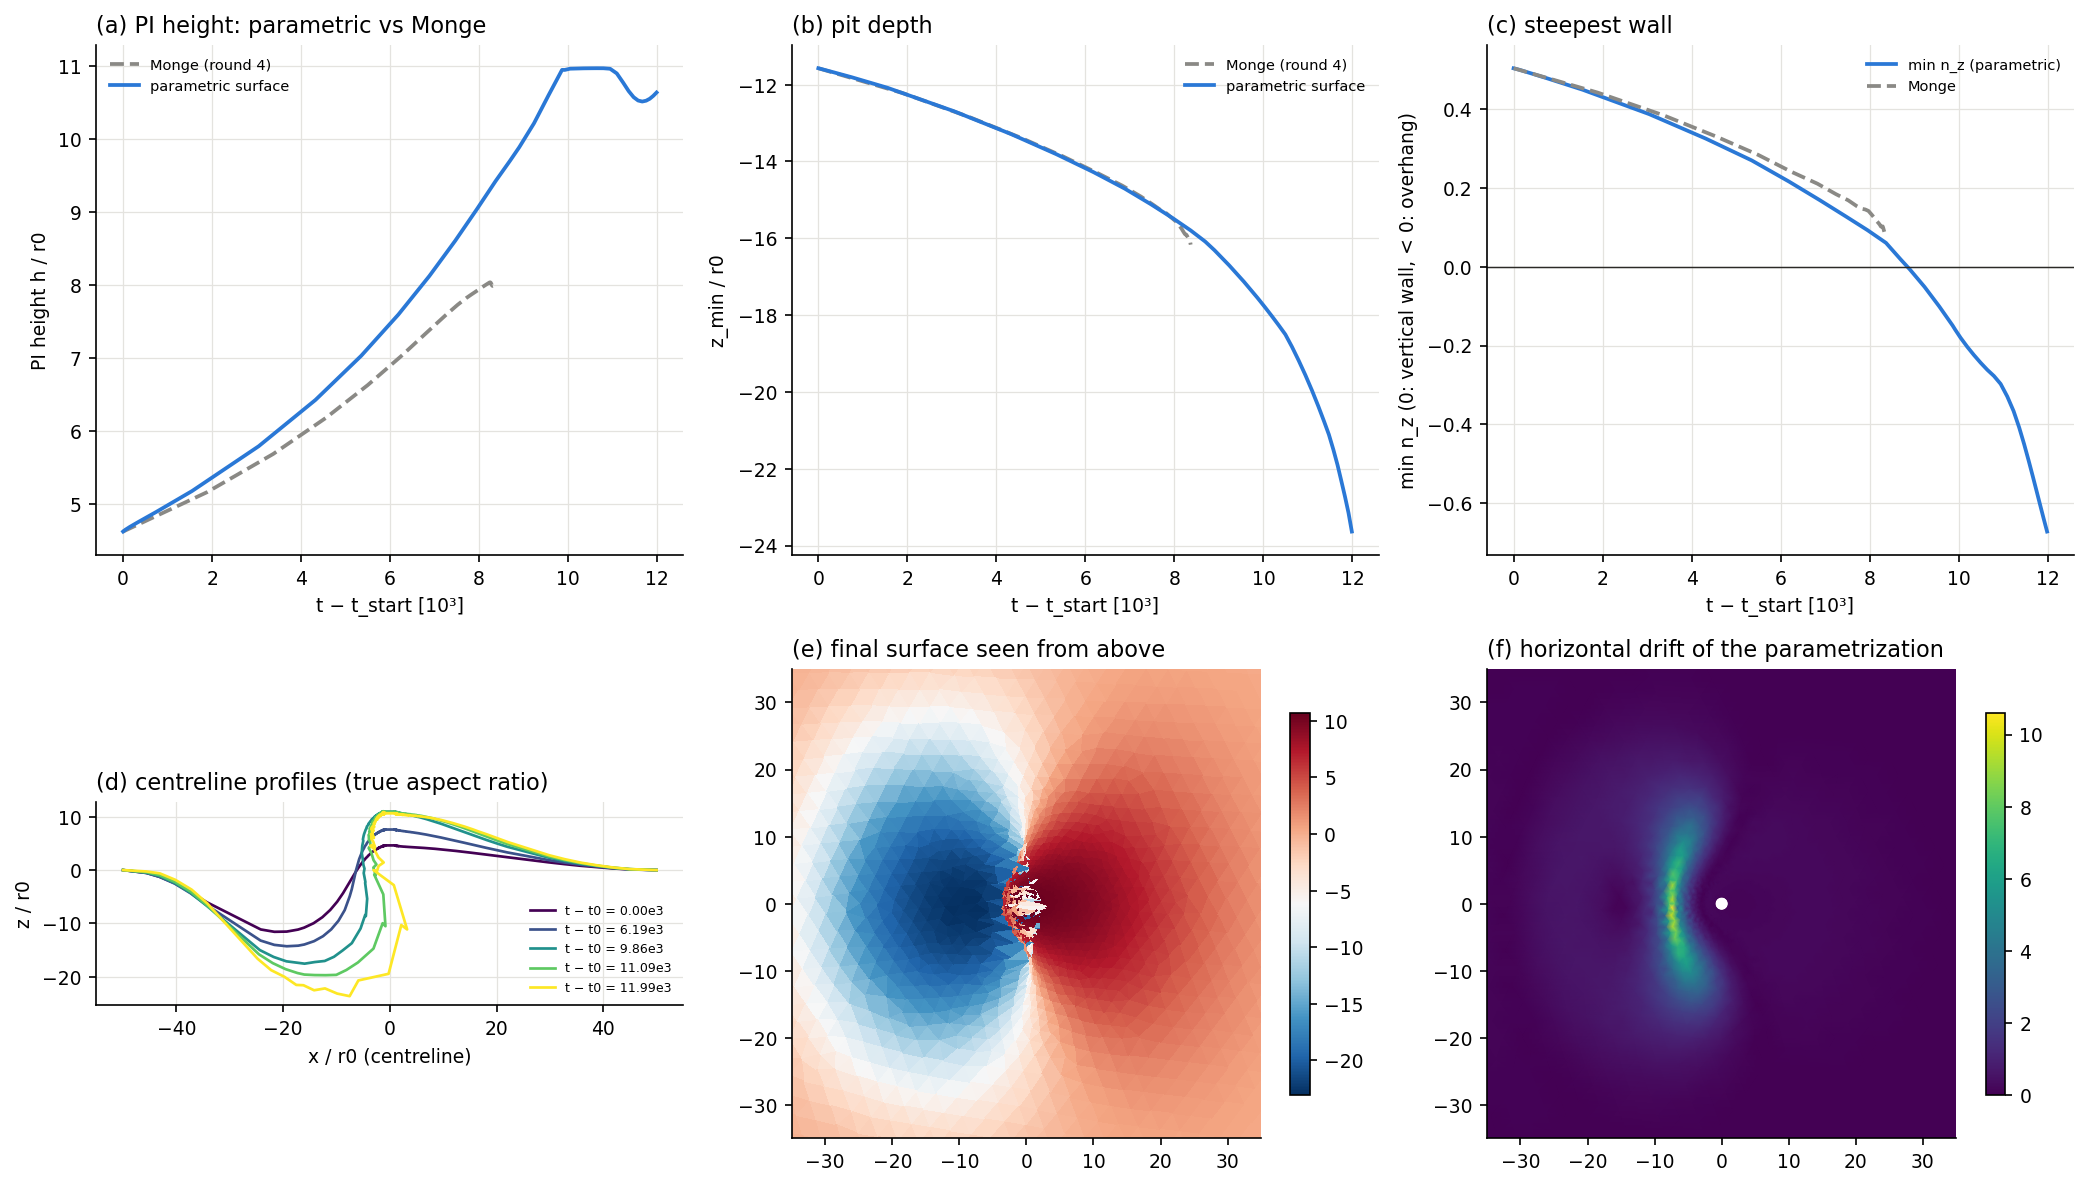
\includegraphics[width=\linewidth,height=175mm,keepaspectratio]{figures/membrane_r5_fold_parametric.png}\captionof{figure}[Main-text figure, larger copy]{Larger copy of main-text Figure 6. Consult its main-text caption for interpretation. \textit{Source:} \path{research/membrane_stability/figures/r5_fold_parametric.png}. First added 2026-10-02.}\end{center}\clearpage
\begin{center}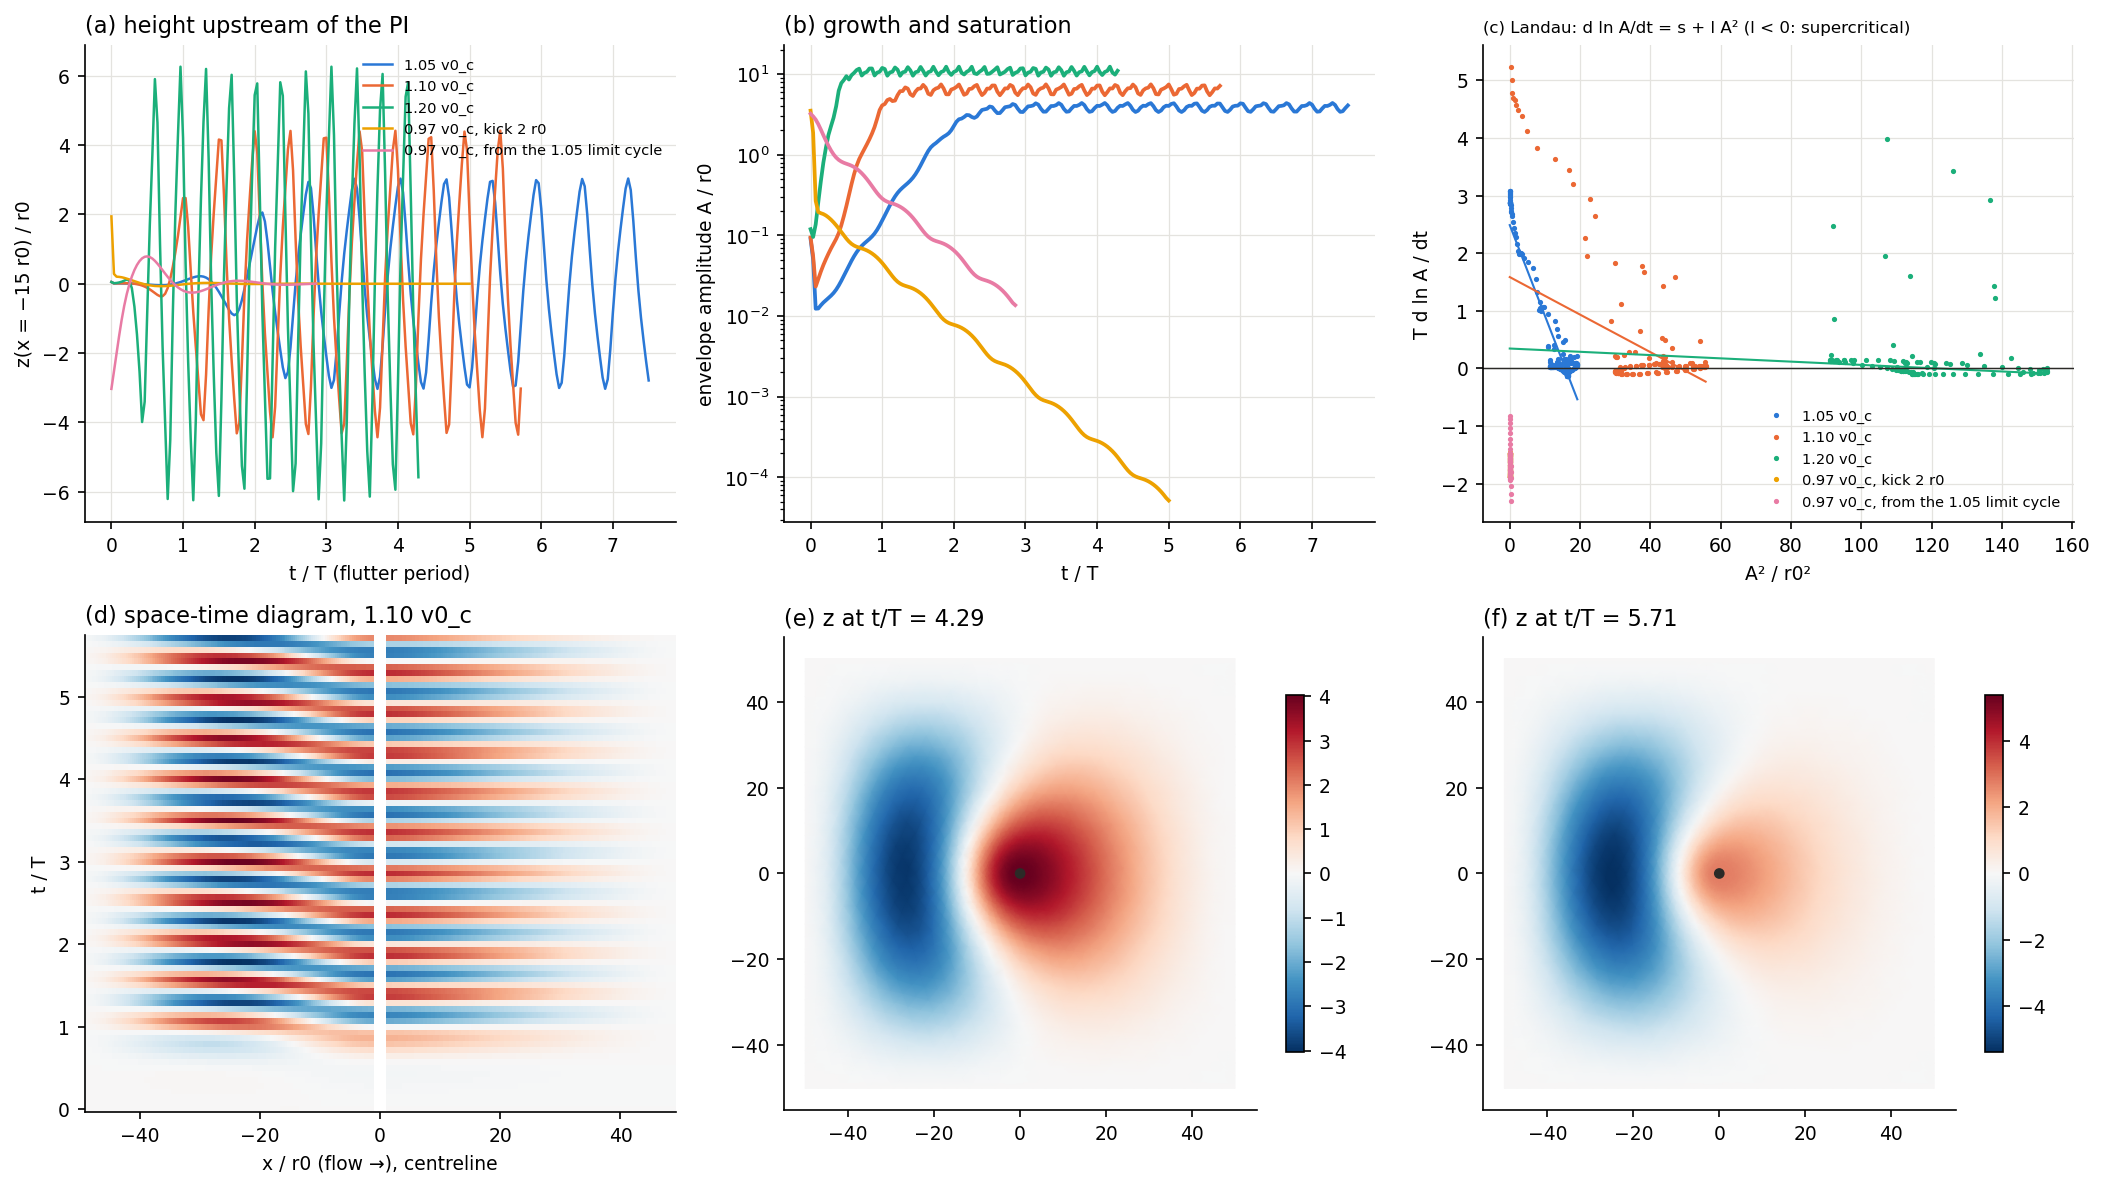
\includegraphics[width=\linewidth,height=175mm,keepaspectratio]{figures/membrane_r5_flutter.png}\captionof{figure}[Main-text figure, larger copy]{Larger copy of main-text Figure 7. Consult its main-text caption for interpretation. \textit{Source:} \path{research/membrane_stability/figures/r5_flutter.png}. First added 2026-10-02.}\end{center}\clearpage
\begin{center}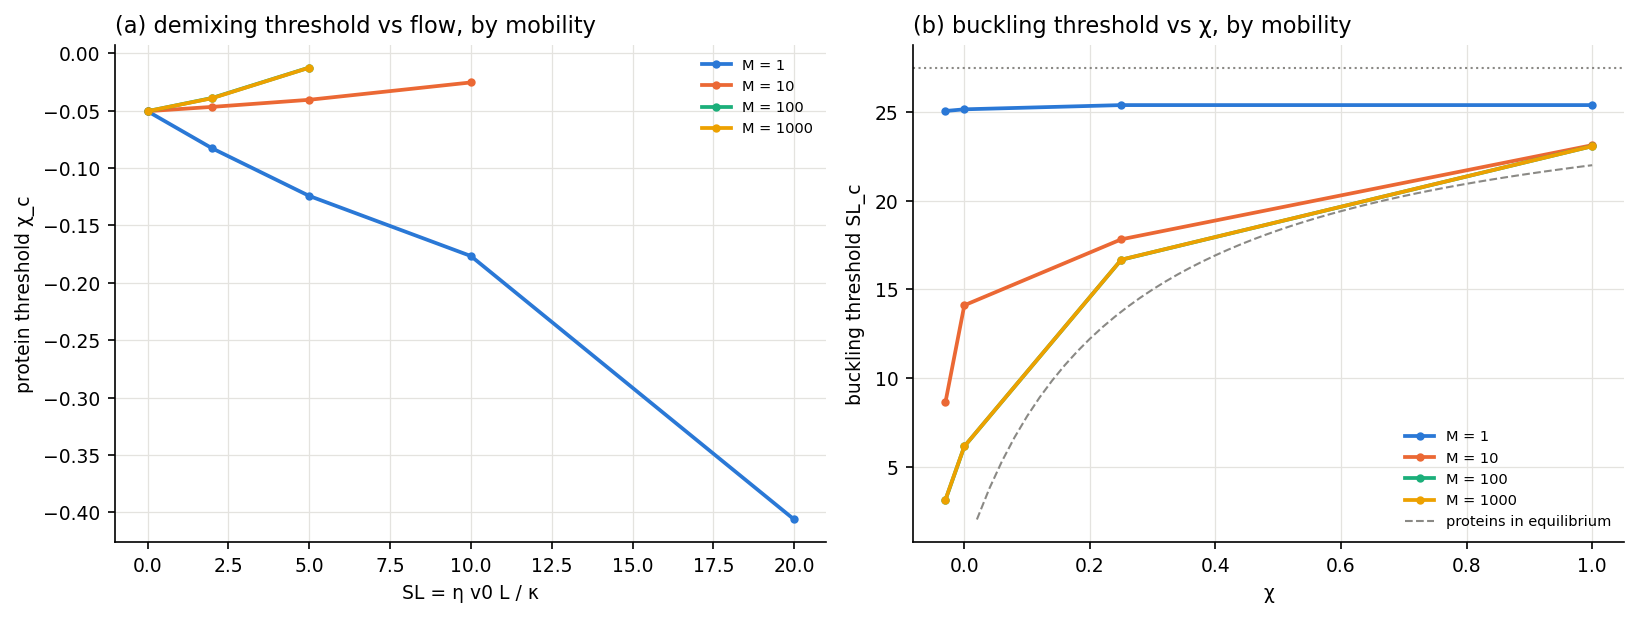
\includegraphics[width=\linewidth,height=175mm,keepaspectratio]{figures/membrane_r5_peclet.png}\captionof{figure}[Main-text figure, larger copy]{Larger copy of main-text Figure 8. Consult its main-text caption for interpretation. \textit{Source:} \path{research/membrane_stability/figures/r5_peclet.png}. First added 2026-10-02.}\end{center}\clearpage
\begin{center}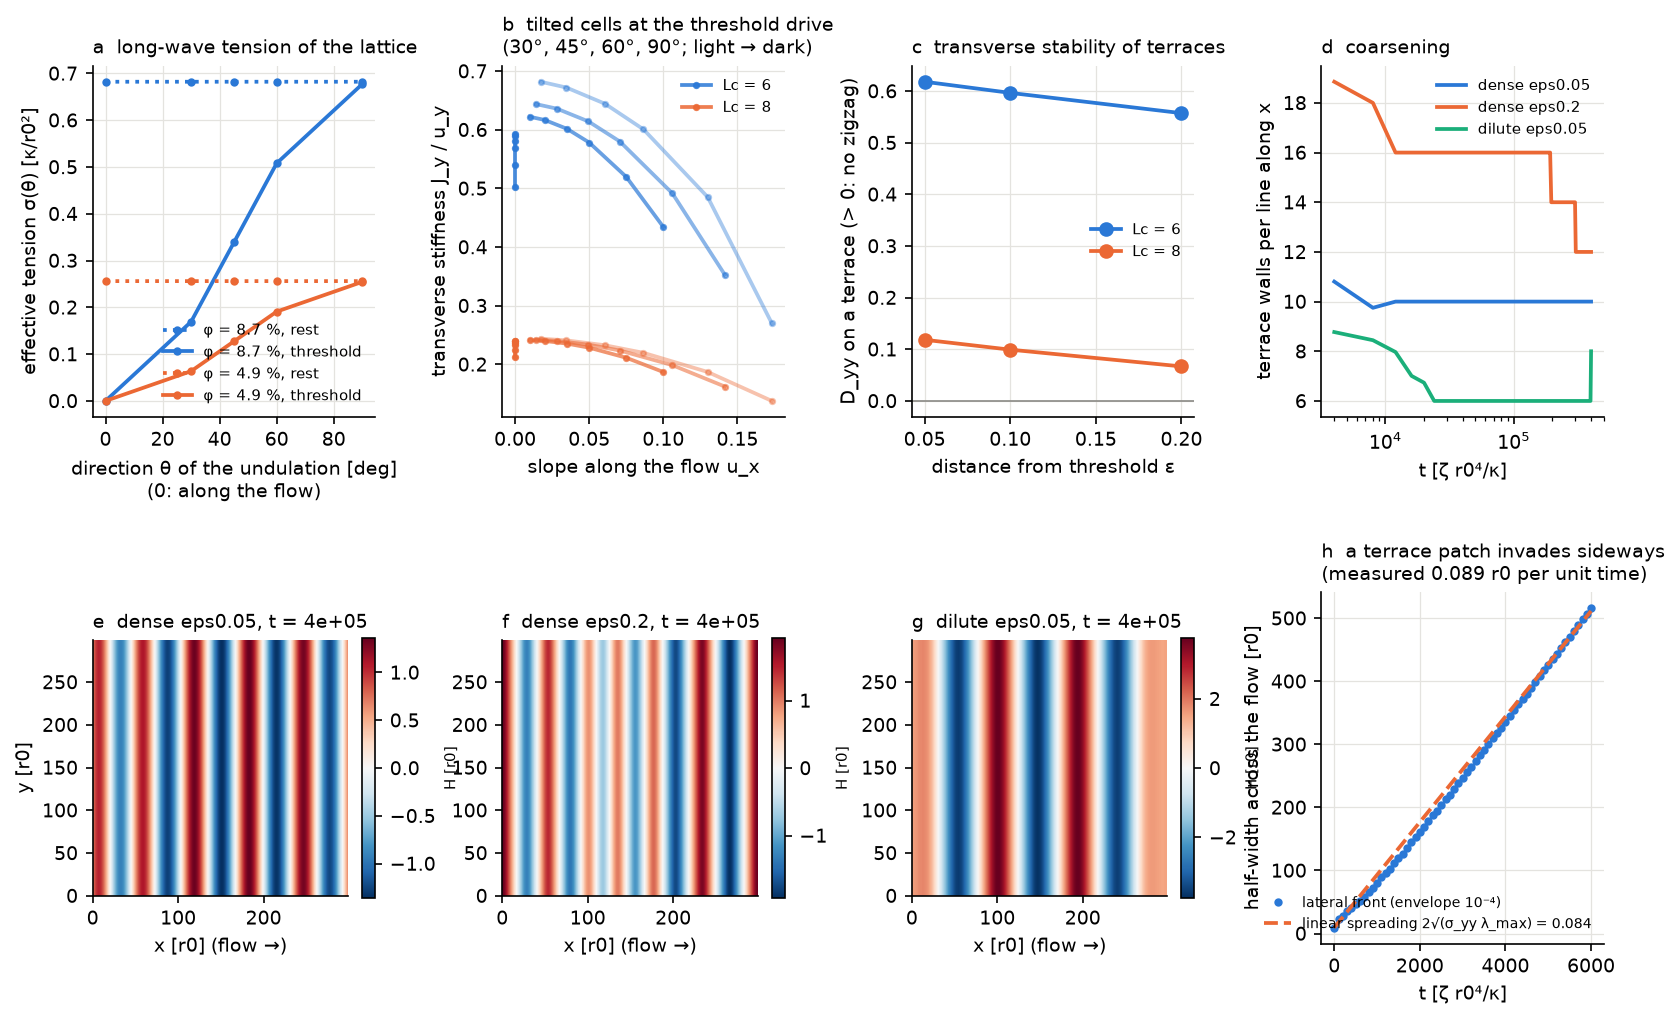
\includegraphics[width=\linewidth,height=175mm,keepaspectratio]{figures/membrane_r6_slope2d.png}\captionof{figure}[Main-text figure, larger copy]{Larger copy of main-text Figure 9. Consult its main-text caption for interpretation. \textit{Source:} \path{research/membrane_stability/figures/r6_slope2d.png}. First added 2026-10-03.}\end{center}\clearpage

\clearpage
\begin{thebibliography}{10}
\bibitem{irene} D. W\"orthm\"uller, G. Ferraro, P. Sens, and M. Castellana, \emph{IRENE: a fluId layeR finitE-elemeNt softwarE}, arXiv:2506.17827 (2025), version 3. \href{https://arxiv.org/abs/2506.17827}{arxiv.org/abs/2506.17827}.
\bibitem{ferraro} G. Ferraro and M. Castellana, \emph{Interaction between cell membranes and protein inclusions in the large-deformation regime}, arXiv:2601.15477 (2026), version 2. \href{https://arxiv.org/abs/2601.15477}{arxiv.org/abs/2601.15477}.
\bibitem{helfrich} W. Helfrich, \emph{Elastic properties of lipid bilayers: Theory and possible experiments}, Z. Naturforsch. C \textbf{28}, 693--703 (1973). \href{https://doi.org/10.1515/znc-1973-11-1209}{doi:10.1515/znc-1973-11-1209}.
\bibitem{tethers} I. Der\'enyi, F. J\"ulicher, and J. Prost, \emph{Formation and interaction of membrane tubes}, Phys. Rev. Lett. \textbf{88}, 238101 (2002). \href{https://doi.org/10.1103/PhysRevLett.88.238101}{doi:10.1103/PhysRevLett.88.238101}.
\bibitem{wake} F. Giannetti and P. Luchini, \emph{Structural sensitivity of the first instability of the cylinder wake}, J. Fluid Mech. \textbf{581}, 167--197 (2007). \href{https://doi.org/10.1017/S0022112007005654}{doi:10.1017/S0022112007005654}.
\bibitem{slepc} V. Hern\'andez, J. E. Rom\'an, and V. Vidal, \emph{SLEPc: A scalable and flexible toolkit for the solution of eigenvalue problems}, ACM Trans. Math. Softw. \textbf{31}, 351--362 (2005). \href{https://slepc.upv.es/release/material/index.html}{SLEPc publications and software}.
\bibitem{leibler} S. Leibler, \emph{Curvature instability in membranes}, J. Phys. France \textbf{47}, 507--516 (1986). \href{https://doi.org/10.1051/jphys:01986004703050700}{doi:10.1051/jphys:01986004703050700}.
\bibitem{huerre} P. Huerre and P. A. Monkewitz, \emph{Local and global instabilities in spatially developing flows}, Annu. Rev. Fluid Mech. \textbf{22}, 473--537 (1990). \href{https://doi.org/10.1146/annurev.fl.22.010190.002353}{doi:10.1146/annurev.fl.22.010190.002353}.
\bibitem{repo} \emph{Copy\_Stage}, repository snapshot \source{45d54f29909d4026ece901c28287b23104190b1d}, 4 October 2026. \href{https://github.com/heiriru/Copy_Stage/tree/45d54f29909d4026ece901c28287b23104190b1d/Ruben/membrane_stability}{Code, archived numerical outputs, and interpretation}. Unless attributed otherwise, all numerical results and figures in this report come from this snapshot.
\end{thebibliography}

\end{document}
